%%%%%%%%%%%%%%%%%%%%%%%%%%%%%%%%%%%%%%%%%
% Masters/Doctoral Thesis 
% LaTeX Template
% Version 2.5 (27/8/17)
%
% This template was downloaded from:
% http://www.LaTeXTemplates.com
%
% Version 2.x major modifications by:
% Vel (vel@latextemplates.com)
%
% This template is based on a template by:
% Steve Gunn (http://users.ecs.soton.ac.uk/srg/softwaretools/document/templates/)
% Sunil Patel (http://www.sunilpatel.co.uk/thesis-template/)
%
% Template license:
% CC BY-NC-SA 3.0 (http://creativecommons.org/licenses/by-nc-sa/3.0/)
%
%%%%%%%%%%%%%%%%%%%%%%%%%%%%%%%%%%%%%%%%%

%----------------------------------------------------------------------------------------
%	PACKAGES AND OTHER DOCUMENT CONFIGURATIONS
%----------------------------------------------------------------------------------------

\documentclass[
12pt, % The default document font size, options: 10pt, 11pt, 12pt
%oneside, % Two side (alternating margins) for binding by default, uncomment to switch to one side
english, % ngerman for German
singlespacing, % Single line spacing, alternatives: onehalfspacing or doublespacing
%draft, % Uncomment to enable draft mode (no pictures, no links, overfull hboxes indicated)
%nolistspacing, % If the document is onehalfspacing or doublespacing, uncomment this to set spacing in lists to single
%liststotoc, % Uncomment to add the list of figures/tables/etc to the table of contents
%toctotoc, % Uncomment to add the main table of contents to the table of contents
%parskip, % Uncomment to add space between paragraphs
%nohyperref, % Uncomment to not load the hyperref package
headsepline, % Uncomment to get a line under the header
%chapterinoneline, % Uncomment to place the chapter title next to the number on one line
%consistentlayout, % Uncomment to change the layout of the declaration, abstract and acknowledgements pages to match the default layout
]{MastersDoctoralThesis} % The class file specifying the document structure

\usepackage[utf8]{inputenc} % Required for inputting international characters
\usepackage[T1]{fontenc} % Output font encoding for international characters
\usepackage{svg}
\usepackage{mathpazo} % Use the Palatino font by default
\usepackage{float}
\usepackage{graphicx}
\usepackage{caption}
\usepackage{subcaption} % para subfiguras
\usepackage{multirow}
\usepackage{colortbl}
\usepackage{longtable}
\usepackage{amsmath}
\usepackage{siunitx}
\usepackage{makecell}
\usepackage{soul}
\usepackage[
  backend=bibtex,       % o 'bibtex' si prefieres
  style=authoryear,          % estilo similar a ieeetr
  sorting=none         % orden de aparición, si lo deseas
]{biblatex}

\usepackage{tabularx} 
\newcolumntype{C}{>{\centering\arraybackslash}X}  % columna centrada y extensible


% \usepackage[backend=bibtex,style=authoryear,natbib=true]{biblatex} % Use the bibtex backend with the authoryear citation style (which resembles APA)

\addbibresource{references.bib} % The filename of the bibliography

\usepackage[autostyle=true]{csquotes} % Required to generate language-dependent quotes in the bibliography

%----------------------------------------------------------------------------------------
%	MARGIN SETTINGS
%----------------------------------------------------------------------------------------

\geometry{
	paper=a4paper, % Change to letterpaper for US letter
	inner=2.5cm, % Inner margin
	outer=3.8cm, % Outer margin
	bindingoffset=.5cm, % Binding offset
	top=1.5cm, % Top margin
	bottom=1.5cm, % Bottom margin
	%showframe, % Uncomment to show how the type block is set on the page
}

%----------------------------------------------------------------------------------------
%	THESIS INFORMATION
%----------------------------------------------------------------------------------------

\thesistitle{Design and Development of a Multispectral Imagery System for Land Cover and Land Use Monitoring in Colombia} % Your thesis title, this is used in the title and abstract, print it elsewhere with \ttitle
\supervisor{PhD. Olga Lucia \textsc{Quintero Montoya}} % Your supervisor's name, this is used in the title page, print it elsewhere with \supname
\examiner{} % Your examiner's name, this is not currently used anywhere in the template, print it elsewhere with \examname
\degree{Maestría en Ciencias} % Your degree name, this is used in the title page and abstract, print it elsewhere with \degreename
\author{Sebastian \textsc{Carmona Estrada}} % Your name, this is used in the title page and abstract, print it elsewhere with \authorname
\addresses{} % Your address, this is not currently used anywhere in the template, print it elsewhere with \addressname

\subject{Biological Sciences} % Your subject area, this is not currently used anywhere in the template, print it elsewhere with \subjectname
\keywords{} % Keywords for your thesis, this is not currently used anywhere in the template, print it elsewhere with \keywordnames
\university{\href{http://www.university.com}{Universidad EAFIT}} % Your university's name and URL, this is used in the title page and abstract, print it elsewhere with \univname
\department{\href{http://department.university.com}{Escuela de Ciencias Aplicadas e Ingeniería}} % Your department's name and URL, this is used in the title page and abstract, print it elsewhere with \deptname
\group{\href{http://researchgroup.university.com}{HuMath}} % Your research group's name and URL, this is used in the title page, print it elsewhere with \groupname
\faculty{\href{http://faculty.university.com}{Maestría en Física Aplicada}} % Your faculty's name and URL, this is used in the title page and abstract, print it elsewhere with \facname

\AtBeginDocument{
\hypersetup{pdftitle=\ttitle} % Set the PDF's title to your title
\hypersetup{pdfauthor=\authorname} % Set the PDF's author to your name
\hypersetup{pdfkeywords=\keywordnames} % Set the PDF's keywords to your keywords
}

\begin{document}

\frontmatter % Use roman page numbering style (i, ii, iii, iv...) for the pre-content pages

\pagestyle{plain} % Default to the plain heading style until the thesis style is called for the body content

%----------------------------------------------------------------------------------------
%	TITLE PAGE
%----------------------------------------------------------------------------------------

\begin{titlepage}
\begin{center}

\vspace*{.06\textheight}
{\scshape\LARGE \univname\par}\vspace{1.5cm} % University name
\textsc{\Large Tésis de Maestría}\\[0.5cm] % Thesis type

\HRule \\[0.4cm] % Horizontal line
{\huge \bfseries \ttitle\par}\vspace{0.4cm} % Thesis title
\HRule \\[1.5cm] % Horizontal line
 
\begin{minipage}[t]{0.4\textwidth}
\begin{flushleft} \large
\emph{Author:}\\
\href{scarmonae@eafit.edu.co}{\authorname} % Author name - remove the \href bracket to remove the link
\end{flushleft}
\end{minipage}
\begin{minipage}[t]{0.4\textwidth}
\begin{flushright} \large
\emph{Supervisor:} \\
\href{http://www.jamessmith.com}{\supname} % Supervisor name - remove the \href bracket to remove the link  
\end{flushright}
\end{minipage}\\[3cm]
 
\vfill

\large \textit{A thesis submitted in fulfillment of the requirements\\ for the degree of \degreename}\\[0.3cm] % University requirement text
\textit{in the}\\[0.4cm]
\groupname\\\deptname\\[2cm] % Research group name and department name
 
\vfill

{\large \today}\\[4cm] % Date
%\includegraphics{Logo} % University/department logo - uncomment to place it
 
\vfill
\end{center}
\end{titlepage}

%----------------------------------------------------------------------------------------
%	DECLARATION PAGE
%----------------------------------------------------------------------------------------

\begin{declaration}
\addchaptertocentry{\authorshipname} % Add the declaration to the table of contents
\noindent I, \authorname, declare that this thesis titled, \enquote{\ttitle} and the work presented in it are my own. I confirm that:

\begin{itemize} 
\item This work was done wholly or mainly while in candidature for a research degree at this University.
\item Where any part of this thesis has previously been submitted for a degree or any other qualification at this University or any other institution, this has been clearly stated.
\item Where I have consulted the published work of others, this is always clearly attributed.
\item Where I have quoted from the work of others, the source is always given. With the exception of such quotations, this thesis is entirely my own work.
\item I have acknowledged all main sources of help.
\item Where the thesis is based on work done by myself jointly with others, I have made clear exactly what was done by others and what I have contributed myself.\\
\end{itemize}
 
\noindent Signed:\\
\rule[0.5em]{25em}{0.5pt} % This prints a line for the signature
 
\noindent Date:\\
\rule[0.5em]{25em}{0.5pt} % This prints a line to write the date
\end{declaration}

\cleardoublepage

%----------------------------------------------------------------------------------------
%	QUOTATION PAGE
%----------------------------------------------------------------------------------------

\vspace*{0.2\textheight}

\noindent\enquote{\itshape Thanks to my solid academic training, today I can write hundreds of words on virtually any topic without possessing a shred of information, which is how I got a good job in journalism.}\bigbreak

\hfill Dave Barry

%----------------------------------------------------------------------------------------
%	ABSTRACT PAGE
%----------------------------------------------------------------------------------------

\begin{abstract}
\addchaptertocentry{\abstractname} % Add the abstract to the table of contents
The Thesis Abstract is written here (and usually kept to just this page). The page is kept centered vertically so can expand into the blank space above the title too\ldots
\end{abstract}

%----------------------------------------------------------------------------------------
%	ACKNOWLEDGEMENTS
%----------------------------------------------------------------------------------------

\begin{acknowledgements}
\addchaptertocentry{\acknowledgementname} % Add the acknowledgements to the table of contents
The acknowledgments and the people to thank go here, don't forget to include your project advisor\ldots
\end{acknowledgements}

%----------------------------------------------------------------------------------------
%	LIST OF CONTENTS/FIGURES/TABLES PAGES
%----------------------------------------------------------------------------------------

\tableofcontents % Prints the main table of contents

\listoffigures % Prints the list of figures

\listoftables % Prints the list of tables

%----------------------------------------------------------------------------------------
%	ABBREVIATIONS
%----------------------------------------------------------------------------------------

\begin{abbreviations}{ll} % Include a list of abbreviations (a table of two columns)

\textbf{LAH} & \textbf{L}ist \textbf{A}bbreviations \textbf{H}ere\\
\textbf{WSF} & \textbf{W}hat (it) \textbf{S}tands \textbf{F}or\\

\end{abbreviations}

%----------------------------------------------------------------------------------------
%	PHYSICAL CONSTANTS/OTHER DEFINITIONS
%----------------------------------------------------------------------------------------

\begin{constants}{lr@{${}={}$}l} % The list of physical constants is a three column table

% The \SI{}{} command is provided by the siunitx package, see its documentation for instructions on how to use it

Speed of Light & $c_{0}$ & \SI{2.99792458e8}{\meter\per\second} (exact)\\
%Constant Name & $Symbol$ & $Constant Value$ with units\\

\end{constants}

%----------------------------------------------------------------------------------------
%	SYMBOLS
%----------------------------------------------------------------------------------------

\begin{symbols}{lll} % Include a list of Symbols (a three column table)

$a$ & distance & \si{\meter} \\
$P$ & power & \si{\watt} (\si{\joule\per\second}) \\
%Symbol & Name & Unit \\

\addlinespace % Gap to separate the Roman symbols from the Greek

$\omega$ & angular frequency & \si{\radian} \\

\end{symbols}

%----------------------------------------------------------------------------------------
%	DEDICATION
%----------------------------------------------------------------------------------------

\dedicatory{For/Dedicated to/To my\ldots} 

%----------------------------------------------------------------------------------------
%	THESIS CONTENT - CHAPTERS
%----------------------------------------------------------------------------------------

\mainmatter % Begin numeric (1,2,3...) page numbering

\pagestyle{thesis} % Return the page headers back to the "thesis" sty

% Include the chapters of the thesis as separate files from the Chapters folder
% Uncomment the lines as you write the chapters

% % % % Chapter 1

% % \chapter{Chapter Title Here} % Main chapter title

% % \label{Chapter1} % For referencing the chapter elsewhere, use \ref{Chapter1} 

% % %----------------------------------------------------------------------------------------

% % % Define some commands to keep the formatting separated from the content 
% % \newcommand{\keyword}[1]{\textbf{#1}}
% % \newcommand{\tabhead}[1]{\textbf{#1}}
% % \newcommand{\code}[1]{\texttt{#1}}
% % \newcommand{\file}[1]{\texttt{\bfseries#1}}
% % \newcommand{\option}[1]{\texttt{\itshape#1}}

% % %----------------------------------------------------------------------------------------

% % \section{Welcome and Thank You}
% % Welcome to this \LaTeX{} Thesis Template, a beautiful and easy to use template for writing a thesis using the \LaTeX{} typesetting system.

% % If you are writing a thesis (or will be in the future) and its subject is technical or mathematical (though it doesn't have to be), then creating it in \LaTeX{} is highly recommended as a way to make sure you can just get down to the essential writing without having to worry over formatting or wasting time arguing with your word processor. 

% % \LaTeX{} is easily able to professionally typeset documents that run to hundreds or thousands of pages long. With simple mark-up commands, it automatically sets out the table of contents, margins, page headers and footers and keeps the formatting consistent and beautiful. One of its main strengths is the way it can easily typeset mathematics, even \emph{heavy} mathematics. Even if those equations are the most horribly twisted and most difficult mathematical problems that can only be solved on a super-computer, you can at least count on \LaTeX{} to make them look stunning.

% % %----------------------------------------------------------------------------------------

% % \section{Learning \LaTeX{}}

% % \LaTeX{} is not a \textsc{wysiwyg} (What You See is What You Get) program, unlike word processors such as Microsoft Word or Apple's Pages. Instead, a document written for \LaTeX{} is actually a simple, plain text file that contains \emph{no formatting}. You tell \LaTeX{} how you want the formatting in the finished document by writing in simple commands amongst the text, for example, if I want to use \emph{italic text for emphasis}, I write the \verb|\emph{text}| command and put the text I want in italics in between the curly braces. This means that \LaTeX{} is a \enquote{mark-up} language, very much like HTML.

% % \subsection{A (not so short) Introduction to \LaTeX{}}

% % If you are new to \LaTeX{}, there is a very good eBook -- freely available online as a PDF file -- called, \enquote{The Not So Short Introduction to \LaTeX{}}. The book's title is typically shortened to just \emph{lshort}. You can download the latest version (as it is occasionally updated) from here:
% % \url{http://www.ctan.org/tex-archive/info/lshort/english/lshort.pdf}

% % It is also available in several other languages. Find yours from the list on this page: \url{http://www.ctan.org/tex-archive/info/lshort/}

% % It is recommended to take a little time out to learn how to use \LaTeX{} by creating several, small `test' documents, or having a close look at several templates on:\\ 
% % \url{http://www.LaTeXTemplates.com}\\ 
% % Making the effort now means you're not stuck learning the system when what you \emph{really} need to be doing is writing your thesis.

% % \subsection{A Short Math Guide for \LaTeX{}}

% % If you are writing a technical or mathematical thesis, then you may want to read the document by the AMS (American Mathematical Society) called, \enquote{A Short Math Guide for \LaTeX{}}. It can be found online here:
% % \url{http://www.ams.org/tex/amslatex.html}
% % under the \enquote{Additional Documentation} section towards the bottom of the page.

% % \subsection{Common \LaTeX{} Math Symbols}
% % There are a multitude of mathematical symbols available for \LaTeX{} and it would take a great effort to learn the commands for them all. The most common ones you are likely to use are shown on this page:
% % \url{http://www.sunilpatel.co.uk/latex-type/latex-math-symbols/}

% % You can use this page as a reference or crib sheet, the symbols are rendered as large, high quality images so you can quickly find the \LaTeX{} command for the symbol you need.

% % \subsection{\LaTeX{} on a Mac}
 
% % The \LaTeX{} distribution is available for many systems including Windows, Linux and Mac OS X. The package for OS X is called MacTeX and it contains all the applications you need -- bundled together and pre-customized -- for a fully working \LaTeX{} environment and work flow.
 
% % MacTeX includes a custom dedicated \LaTeX{} editor called TeXShop for writing your `\file{.tex}' files and BibDesk: a program to manage your references and create your bibliography section just as easily as managing songs and creating playlists in iTunes.

% % %----------------------------------------------------------------------------------------

% % \section{Getting Started with this Template}

% % If you are familiar with \LaTeX{}, then you should explore the directory structure of the template and then proceed to place your own information into the \emph{THESIS INFORMATION} block of the \file{main.tex} file. You can then modify the rest of this file to your unique specifications based on your degree/university. Section \ref{FillingFile} on page \pageref{FillingFile} will help you do this. Make sure you also read section \ref{ThesisConventions} about thesis conventions to get the most out of this template.

% % If you are new to \LaTeX{} it is recommended that you carry on reading through the rest of the information in this document.

% % Before you begin using this template you should ensure that its style complies with the thesis style guidelines imposed by your institution. In most cases this template style and layout will be suitable. If it is not, it may only require a small change to bring the template in line with your institution's recommendations. These modifications will need to be done on the \file{MastersDoctoralThesis.cls} file.

% % \subsection{About this Template}

% % This \LaTeX{} Thesis Template is originally based and created around a \LaTeX{} style file created by Steve R.\ Gunn from the University of Southampton (UK), department of Electronics and Computer Science. You can find his original thesis style file at his site, here:
% % \url{http://www.ecs.soton.ac.uk/~srg/softwaretools/document/templates/}

% % Steve's \file{ecsthesis.cls} was then taken by Sunil Patel who modified it by creating a skeleton framework and folder structure to place the thesis files in. The resulting template can be found on Sunil's site here:
% % \url{http://www.sunilpatel.co.uk/thesis-template}

% % Sunil's template was made available through \url{http://www.LaTeXTemplates.com} where it was modified many times based on user requests and questions. Version 2.0 and onwards of this template represents a major modification to Sunil's template and is, in fact, hardly recognisable. The work to make version 2.0 possible was carried out by \href{mailto:vel@latextemplates.com}{Vel} and Johannes Böttcher.

% % %----------------------------------------------------------------------------------------

% % \section{What this Template Includes}

% % \subsection{Folders}

% % This template comes as a single zip file that expands out to several files and folders. The folder names are mostly self-explanatory:

% % \keyword{Appendices} -- this is the folder where you put the appendices. Each appendix should go into its own separate \file{.tex} file. An example and template are included in the directory.

% % \keyword{Chapters} -- this is the folder where you put the thesis chapters. A thesis usually has about six chapters, though there is no hard rule on this. Each chapter should go in its own separate \file{.tex} file and they can be split as:
% % \begin{itemize}
% % \item Chapter 1: Introduction to the thesis topic
% % \item Chapter 2: Background information and theory
% % \item Chapter 3: (Laboratory) experimental setup
% % \item Chapter 4: Details of experiment 1
% % \item Chapter 5: Details of experiment 2
% % \item Chapter 6: Discussion of the experimental results
% % \item Chapter 7: Conclusion and future directions
% % \end{itemize}
% % This chapter layout is specialised for the experimental sciences, your discipline may be different.

% % \keyword{Figures} -- this folder contains all figures for the thesis. These are the final images that will go into the thesis document.

% % \subsection{Files}

% % Included are also several files, most of them are plain text and you can see their contents in a text editor. After initial compilation, you will see that more auxiliary files are created by \LaTeX{} or BibTeX and which you don't need to delete or worry about:

% % \keyword{example.bib} -- this is an important file that contains all the bibliographic information and references that you will be citing in the thesis for use with BibTeX. You can write it manually, but there are reference manager programs available that will create and manage it for you. Bibliographies in \LaTeX{} are a large subject and you may need to read about BibTeX before starting with this. Many modern reference managers will allow you to export your references in BibTeX format which greatly eases the amount of work you have to do.

% % \keyword{MastersDoctoralThesis.cls} -- this is an important file. It is the class file that tells \LaTeX{} how to format the thesis. 

% % \keyword{main.pdf} -- this is your beautifully typeset thesis (in the PDF file format) created by \LaTeX{}. It is supplied in the PDF with the template and after you compile the template you should get an identical version.

% % \keyword{main.tex} -- this is an important file. This is the file that you tell \LaTeX{} to compile to produce your thesis as a PDF file. It contains the framework and constructs that tell \LaTeX{} how to layout the thesis. It is heavily commented so you can read exactly what each line of code does and why it is there. After you put your own information into the \emph{THESIS INFORMATION} block -- you have now started your thesis!

% % Files that are \emph{not} included, but are created by \LaTeX{} as auxiliary files include:

% % \keyword{main.aux} -- this is an auxiliary file generated by \LaTeX{}, if it is deleted \LaTeX{} simply regenerates it when you run the main \file{.tex} file.

% % \keyword{main.bbl} -- this is an auxiliary file generated by BibTeX, if it is deleted, BibTeX simply regenerates it when you run the \file{main.aux} file. Whereas the \file{.bib} file contains all the references you have, this \file{.bbl} file contains the references you have actually cited in the thesis and is used to build the bibliography section of the thesis.

% % \keyword{main.blg} -- this is an auxiliary file generated by BibTeX, if it is deleted BibTeX simply regenerates it when you run the main \file{.aux} file.

% % \keyword{main.lof} -- this is an auxiliary file generated by \LaTeX{}, if it is deleted \LaTeX{} simply regenerates it when you run the main \file{.tex} file. It tells \LaTeX{} how to build the \emph{List of Figures} section.

% % \keyword{main.log} -- this is an auxiliary file generated by \LaTeX{}, if it is deleted \LaTeX{} simply regenerates it when you run the main \file{.tex} file. It contains messages from \LaTeX{}, if you receive errors and warnings from \LaTeX{}, they will be in this \file{.log} file.

% % \keyword{main.lot} -- this is an auxiliary file generated by \LaTeX{}, if it is deleted \LaTeX{} simply regenerates it when you run the main \file{.tex} file. It tells \LaTeX{} how to build the \emph{List of Tables} section.

% % \keyword{main.out} -- this is an auxiliary file generated by \LaTeX{}, if it is deleted \LaTeX{} simply regenerates it when you run the main \file{.tex} file.

% % So from this long list, only the files with the \file{.bib}, \file{.cls} and \file{.tex} extensions are the most important ones. The other auxiliary files can be ignored or deleted as \LaTeX{} and BibTeX will regenerate them.

% % %----------------------------------------------------------------------------------------

% % \section{Filling in Your Information in the \file{main.tex} File}\label{FillingFile}

% % You will need to personalise the thesis template and make it your own by filling in your own information. This is done by editing the \file{main.tex} file in a text editor or your favourite LaTeX environment.

% % Open the file and scroll down to the third large block titled \emph{THESIS INFORMATION} where you can see the entries for \emph{University Name}, \emph{Department Name}, etc \ldots

% % Fill out the information about yourself, your group and institution. You can also insert web links, if you do, make sure you use the full URL, including the \code{http://} for this. If you don't want these to be linked, simply remove the \verb|\href{url}{name}| and only leave the name.

% % When you have done this, save the file and recompile \code{main.tex}. All the information you filled in should now be in the PDF, complete with web links. You can now begin your thesis proper!

% % %----------------------------------------------------------------------------------------

% % \section{The \code{main.tex} File Explained}

% % The \file{main.tex} file contains the structure of the thesis. There are plenty of written comments that explain what pages, sections and formatting the \LaTeX{} code is creating. Each major document element is divided into commented blocks with titles in all capitals to make it obvious what the following bit of code is doing. Initially there seems to be a lot of \LaTeX{} code, but this is all formatting, and it has all been taken care of so you don't have to do it.

% % Begin by checking that your information on the title page is correct. For the thesis declaration, your institution may insist on something different than the text given. If this is the case, just replace what you see with what is required in the \emph{DECLARATION PAGE} block.

% % Then comes a page which contains a funny quote. You can put your own, or quote your favourite scientist, author, person, and so on. Make sure to put the name of the person who you took the quote from.

% % Following this is the abstract page which summarises your work in a condensed way and can almost be used as a standalone document to describe what you have done. The text you write will cause the heading to move up so don't worry about running out of space.

% % Next come the acknowledgements. On this page, write about all the people who you wish to thank (not forgetting parents, partners and your advisor/supervisor).

% % The contents pages, list of figures and tables are all taken care of for you and do not need to be manually created or edited. The next set of pages are more likely to be optional and can be deleted since they are for a more technical thesis: insert a list of abbreviations you have used in the thesis, then a list of the physical constants and numbers you refer to and finally, a list of mathematical symbols used in any formulae. Making the effort to fill these tables means the reader has a one-stop place to refer to instead of searching the internet and references to try and find out what you meant by certain abbreviations or symbols.

% % The list of symbols is split into the Roman and Greek alphabets. Whereas the abbreviations and symbols ought to be listed in alphabetical order (and this is \emph{not} done automatically for you) the list of physical constants should be grouped into similar themes.

% % The next page contains a one line dedication. Who will you dedicate your thesis to?

% % Finally, there is the block where the chapters are included. Uncomment the lines (delete the \code{\%} character) as you write the chapters. Each chapter should be written in its own file and put into the \emph{Chapters} folder and named \file{Chapter1}, \file{Chapter2}, etc\ldots Similarly for the appendices, uncomment the lines as you need them. Each appendix should go into its own file and placed in the \emph{Appendices} folder.

% % After the preamble, chapters and appendices finally comes the bibliography. The bibliography style (called \option{authoryear}) is used for the bibliography and is a fully featured style that will even include links to where the referenced paper can be found online. Do not underestimate how grateful your reader will be to find that a reference to a paper is just a click away. Of course, this relies on you putting the URL information into the BibTeX file in the first place.

% % %----------------------------------------------------------------------------------------

% % \section{Thesis Features and Conventions}\label{ThesisConventions}

% % To get the best out of this template, there are a few conventions that you may want to follow.

% % One of the most important (and most difficult) things to keep track of in such a long document as a thesis is consistency. Using certain conventions and ways of doing things (such as using a Todo list) makes the job easier. Of course, all of these are optional and you can adopt your own method.

% % \subsection{Printing Format}

% % This thesis template is designed for double sided printing (i.e. content on the front and back of pages) as most theses are printed and bound this way. Switching to one sided printing is as simple as uncommenting the \option{oneside} option of the \code{documentclass} command at the top of the \file{main.tex} file. You may then wish to adjust the margins to suit specifications from your institution.

% % The headers for the pages contain the page number on the outer side (so it is easy to flick through to the page you want) and the chapter name on the inner side.

% % The text is set to 11 point by default with single line spacing, again, you can tune the text size and spacing should you want or need to using the options at the very start of \file{main.tex}. The spacing can be changed similarly by replacing the \option{singlespacing} with \option{onehalfspacing} or \option{doublespacing}.

% % \subsection{Using US Letter Paper}

% % The paper size used in the template is A4, which is the standard size in Europe. If you are using this thesis template elsewhere and particularly in the United States, then you may have to change the A4 paper size to the US Letter size. This can be done in the margins settings section in \file{main.tex}.

% % Due to the differences in the paper size, the resulting margins may be different to what you like or require (as it is common for institutions to dictate certain margin sizes). If this is the case, then the margin sizes can be tweaked by modifying the values in the same block as where you set the paper size. Now your document should be set up for US Letter paper size with suitable margins.

% % \subsection{References}

% % The \code{biblatex} package is used to format the bibliography and inserts references such as this one \parencite{Reference1}. The options used in the \file{main.tex} file mean that the in-text citations of references are formatted with the author(s) listed with the date of the publication. Multiple references are separated by semicolons (e.g. \parencite{Reference2, Reference1}) and references with more than three authors only show the first author with \emph{et al.} indicating there are more authors (e.g. \parencite{Reference3}). This is done automatically for you. To see how you use references, have a look at the \file{Chapter1.tex} source file. Many reference managers allow you to simply drag the reference into the document as you type.

% % Scientific references should come \emph{before} the punctuation mark if there is one (such as a comma or period). The same goes for footnotes\footnote{Such as this footnote, here down at the bottom of the page.}. You can change this but the most important thing is to keep the convention consistent throughout the thesis. Footnotes themselves should be full, descriptive sentences (beginning with a capital letter and ending with a full stop). The APA6 states: \enquote{Footnote numbers should be superscripted, [...], following any punctuation mark except a dash.} The Chicago manual of style states: \enquote{A note number should be placed at the end of a sentence or clause. The number follows any punctuation mark except the dash, which it precedes. It follows a closing parenthesis.}

% % The bibliography is typeset with references listed in alphabetical order by the first author's last name. This is similar to the APA referencing style. To see how \LaTeX{} typesets the bibliography, have a look at the very end of this document (or just click on the reference number links in in-text citations).

% % \subsubsection{A Note on bibtex}

% % The bibtex backend used in the template by default does not correctly handle unicode character encoding (i.e. "international" characters). You may see a warning about this in the compilation log and, if your references contain unicode characters, they may not show up correctly or at all. The solution to this is to use the biber backend instead of the outdated bibtex backend. This is done by finding this in \file{main.tex}: \option{backend=bibtex} and changing it to \option{backend=biber}. You will then need to delete all auxiliary BibTeX files and navigate to the template directory in your terminal (command prompt). Once there, simply type \code{biber main} and biber will compile your bibliography. You can then compile \file{main.tex} as normal and your bibliography will be updated. An alternative is to set up your LaTeX editor to compile with biber instead of bibtex, see \href{http://tex.stackexchange.com/questions/154751/biblatex-with-biber-configuring-my-editor-to-avoid-undefined-citations/}{here} for how to do this for various editors.

% % \subsection{Tables}

% % Tables are an important way of displaying your results, below is an example table which was generated with this code:

% % {\small
% % \begin{verbatim}
% % \begin{table}
% % \caption{The effects of treatments X and Y on the four groups studied.}
% % \label{tab:treatments}
% % \centering
% % \begin{tabular}{l l l}
% % \toprule
% % \tabhead{Groups} & \tabhead{Treatment X} & \tabhead{Treatment Y} \\
% % \midrule
% % 1 & 0.2 & 0.8\\
% % 2 & 0.17 & 0.7\\
% % 3 & 0.24 & 0.75\\
% % 4 & 0.68 & 0.3\\
% % \bottomrule\\
% % \end{tabular}
% % \end{table}
% % \end{verbatim}
% % }

% % \begin{table}
% % \caption{The effects of treatments X and Y on the four groups studied.}
% % \label{tab:treatments}
% % \centering
% % \begin{tabular}{l l l}
% % \toprule
% % \tabhead{Groups} & \tabhead{Treatment X} & \tabhead{Treatment Y} \\
% % \midrule
% % 1 & 0.2 & 0.8\\
% % 2 & 0.17 & 0.7\\
% % 3 & 0.24 & 0.75\\
% % 4 & 0.68 & 0.3\\
% % \bottomrule\\
% % \end{tabular}
% % \end{table}

% % You can reference tables with \verb|\ref{<label>}| where the label is defined within the table environment. See \file{Chapter1.tex} for an example of the label and citation (e.g. Table~\ref{tab:treatments}).

% % \subsection{Figures}

% % There will hopefully be many figures in your thesis (that should be placed in the \emph{Figures} folder). The way to insert figures into your thesis is to use a code template like this:
% % \begin{verbatim}
% % \begin{figure}
% % \centering
% % 
\includegraphics{Figures/Electron}
% % \decoRule
% % \caption[An Electron]{An electron (artist's impression).}
% % \label{fig:Electron}
% % \end{figure}
% % \end{verbatim}
% % Also look in the source file. Putting this code into the source file produces the picture of the electron that you can see in the figure below.

% % \begin{figure}[th]
% % \centering
% % 
\includegraphics{Figures/Electron}
% % \decoRule
% % \caption[An Electron]{An electron (artist's impression).}
% % \label{fig:Electron}
% % \end{figure}

% % Sometimes figures don't always appear where you write them in the source. The placement depends on how much space there is on the page for the figure. Sometimes there is not enough room to fit a figure directly where it should go (in relation to the text) and so \LaTeX{} puts it at the top of the next page. Positioning figures is the job of \LaTeX{} and so you should only worry about making them look good!

% % Figures usually should have captions just in case you need to refer to them (such as in Figure~\ref{fig:Electron}). The \verb|\caption| command contains two parts, the first part, inside the square brackets is the title that will appear in the \emph{List of Figures}, and so should be short. The second part in the curly brackets should contain the longer and more descriptive caption text.

% % The \verb|\decoRule| command is optional and simply puts an aesthetic horizontal line below the image. If you do this for one image, do it for all of them.

% % \LaTeX{} is capable of using images in pdf, jpg and png format.

% % \subsection{Typesetting mathematics}

% % If your thesis is going to contain heavy mathematical content, be sure that \LaTeX{} will make it look beautiful, even though it won't be able to solve the equations for you.

% % The \enquote{Not So Short Introduction to \LaTeX} (available on \href{http://www.ctan.org/tex-archive/info/lshort/english/lshort.pdf}{CTAN}) should tell you everything you need to know for most cases of typesetting mathematics. If you need more information, a much more thorough mathematical guide is available from the AMS called, \enquote{A Short Math Guide to \LaTeX} and can be downloaded from:
% % \url{ftp://ftp.ams.org/pub/tex/doc/amsmath/short-math-guide.pdf}

% % There are many different \LaTeX{} symbols to remember, luckily you can find the most common symbols in \href{http://ctan.org/pkg/comprehensive}{The Comprehensive \LaTeX~Symbol List}.

% % You can write an equation, which is automatically given an equation number by \LaTeX{} like this:
% % \begin{verbatim}
% % \begin{equation}
% % E = mc^{2}
% % \label{eqn:Einstein}
% % \end{equation}
% % \end{verbatim}

% % This will produce Einstein's famous energy-matter equivalence equation:
% % \begin{equation}
% % E = mc^{2}
% % \label{eqn:Einstein}
% % \end{equation}

% % All equations you write (which are not in the middle of paragraph text) are automatically given equation numbers by \LaTeX{}. If you don't want a particular equation numbered, use the unnumbered form:
% % \begin{verbatim}
% % \[ a^{2}=4 \]
% % \end{verbatim}

% % %----------------------------------------------------------------------------------------

% % \section{Sectioning and Subsectioning}

% % You should break your thesis up into nice, bite-sized sections and subsections. \LaTeX{} automatically builds a table of Contents by looking at all the \verb|\chapter{}|, \verb|\section{}|  and \verb|\subsection{}| commands you write in the source.

% % The Table of Contents should only list the sections to three (3) levels. A \verb|chapter{}| is level zero (0). A \verb|\section{}| is level one (1) and so a \verb|\subsection{}| is level two (2). In your thesis it is likely that you will even use a \verb|subsubsection{}|, which is level three (3). The depth to which the Table of Contents is formatted is set within \file{MastersDoctoralThesis.cls}. If you need this changed, you can do it in \file{main.tex}.

% % %----------------------------------------------------------------------------------------

% % \section{In Closing}

% % You have reached the end of this mini-guide. You can now rename or overwrite this pdf file and begin writing your own \file{Chapter1.tex} and the rest of your thesis. The easy work of setting up the structure and framework has been taken care of for you. It's now your job to fill it out!

% % Good luck and have lots of fun!

% % \begin{flushright}
% % Guide written by ---\\
% % Sunil Patel: \href{http://www.sunilpatel.co.uk}{www.sunilpatel.co.uk}\\
% % Vel: \href{http://www.LaTeXTemplates.com}{LaTeXTemplates.com}
% % \end{flushright}


% % \section{Objetivo General}
% % El objetivo general de esta tesis es el desarrollar un método integral para la evaluación de índices de vegetación utilizando datos de sensado remoto obtenidos a través de cámaras multiespectrales, combinando análisis matemáticos y de procesamiento de imágenes para mejorar la precisión y utilidad de estos índices en aplicaciones de monitoreo ambiental y agrícola.


% % \section{Objetivos específicos}

% % \begin{itemize}
% %     \item Realizar una revisión exhaustiva del estado del arte en índices de vegetación, sensado remoto con cámaras multiespectrales y métodos matemáticos y de procesamiento de imágenes aplicados al análisis de datos ambientales y agrícolas.
% %     \item Seleccionar y adquirir los datos necesarios de sensado remoto mediante cámaras multiespectrales para llevar a cabo el estudio.
% %     \item Desarrollar y validar un algoritmo de procesamiento de imágenes que permita la extracción precisa de información sobre vegetación a partir de los datos recopilados.
% %     \item Comparar diferentes índices de vegetación, como el NDVI, EVI, SAVI, entre otros, para determinar su eficacia en la caracterización y monitoreo de la vegetación en el área de estudio.
% %     \item Aplicar métodos estadísticos y de modelado matemático para analizar la relación entre los índices de vegetación obtenidos y variables ambientales y agrícolas relevantes, como la biomasa, la salud de la vegetación y el rendimiento de los cultivos.
% %     \item Evaluar la precisión y utilidad del método desarrollado en la detección y monitoreo de cambios en la vegetación a lo largo del tiempo y en respuesta a diferentes condiciones ambientales y prácticas de manejo agrícola.
% %     \item Presentar los resultados obtenidos de manera clara y concisa, destacando las contribuciones y aplicaciones potenciales del método propuesto en la toma de decisiones ambientales y agrícolas.

% \chapter{Introducción}

% \section*{Planteamiento del Problema}

% \subsection*{Situación Ideal}

% En un contexto agrícola y ambiental óptimo, es esencial disponer de sistemas de monitoreo continuo y confiable de los índices de vegetación para optimizar la gestión de cultivos, preservar los ecosistemas y enfrentar desafíos como el cambio climático. Tecnologías avanzadas de teledetección deberían permitir la obtención de datos precisos y de alta resolución espacial y temporal, facilitando decisiones informadas y oportunas en el manejo de los recursos naturales.

% \subsection*{Realidad Actual en Colombia}

% Sin embargo, en Colombia, país con una gran biodiversidad y extensas áreas agrícolas, el monitoreo eficiente de los índices de vegetación enfrenta serias limitaciones:

% \begin{itemize}
%     \item \textbf{Escasez de Estudios Locales:} Los estudios sobre índices de vegetación en Colombia son reducidos. Investigaciones como las de \cite{Poveda2001SeasonalityColombia} han abordado la relación entre el fenómeno ENSO y los índices de vegetación, pero se centran más en aspectos climáticos que en el desarrollo de tecnologías de monitoreo . Otros estudios, como el de \cite{Navia2016MultispectralUAV}, han utilizado cámaras NIR montadas en UAVs para evaluar el efecto del nitrógeno en la caña de azúcar, pero son casos específicos y no abarcan una solución generalizada.

%     \item \textbf{Limitaciones de Satélites:} Las condiciones atmosféricas propias del trópico colombiano, como la alta presencia de vapor de agua y nubosidad frecuente, disminuyen la eficacia de los satélites para el monitoreo continuo y confiable de la vegetación. Esto afecta la calidad y disponibilidad de las imágenes satelitales.

%     \item \textbf{Baja Resolución Espacial y Temporal:} Los sistemas satelitales disponibles presentan una resolución espacial y temporal insuficiente para el monitoreo detallado requerido en los ecosistemas y cultivos colombianos. Esto impide detectar cambios rápidos en la vegetación y limita la capacidad de respuesta ante eventos adversos.
% \end{itemize}

% \subsection*{Consecuencias}

% La falta de un monitoreo adecuado de los índices de vegetación tiene múltiples implicaciones negativas:

% \begin{itemize}
%     \item \textbf{Gestión Ineficiente de Cultivos:} Sin información precisa, los agricultores no pueden optimizar prácticas agrícolas, lo que puede conducir a bajas productividades y pérdidas económicas. Por ejemplo, el proyecto AgroTIC buscó mejorar esta situación mediante una aplicación móvil para asistencia técnica y estimación de índices de vegetación, pero evidencia la necesidad de soluciones más robustas \cite{Camacho2018Smartphone-basedAgroTICi}.

%     \item \textbf{Riesgos Ambientales:} La ausencia de datos detallados dificulta la implementación de estrategias de conservación y manejo sostenible de los ecosistemas, aumentando la vulnerabilidad ante el cambio climático y la degradación ambiental.

%     \item \textbf{Limitaciones en la Investigación Científica:} La escasez de estudios y datos locales limita el avance científico y tecnológico en áreas clave como la agronomía, la ecología y la gestión ambiental.
% \end{itemize}

% \subsection*{Problema Central}

% ¿Cómo desarrollar una solución tecnológica que permita el monitoreo continuo, preciso y de alta resolución de los índices de vegetación en Colombia, superando las limitaciones impuestas por las condiciones atmosféricas tropicales y las restricciones de los sistemas satelitales actuales?

% \subsection*{Análisis de Estudios Realizados en Colombia}

% Los pocos estudios disponibles en Colombia han explorado el uso de tecnologías como cámaras NIR y aplicaciones móviles para estimar índices de vegetación:

% \begin{itemize}
%     \item \textbf{Aplicaciones Móviles y TIC:} El proyecto AgroTIC desarrolló una aplicación para asistencia técnica y estimación de índices de vegetación visibles usando smartphones, demostrando el potencial de las TIC en la agricultura colombiana\footnote{Díaz, A., et al. (2018). \textit{Op. cit.}}.

%     \item \textbf{Uso de UAVs con Cámaras NIR:} Navia et al. (2016) evaluaron una cámara NIR montada en un UAV para monitorear el rendimiento y el efecto del nitrógeno en la caña de azúcar, indicando la utilidad de estas tecnologías en aplicaciones agrícolas específicas \cite{Navia2016MultispectralUAV}.

%     \item \textbf{Limitaciones Identificadas:} Estos estudios resaltan las dificultades para obtener datos precisos debido a las condiciones atmosféricas y reconocen la necesidad de tecnologías más avanzadas y adaptadas al contexto local.
% \end{itemize}

% \subsection*{Justificación y Relevancia}

% Desarrollar, calibrar y caracterizar una cámara multiespectral para ser montada en una plataforma UAV representa una solución innovadora y adaptada a las necesidades de Colombia:

% \begin{itemize}
%     \item \textbf{Superación de Limitaciones Atmosféricas:} Al operar por debajo de las nubes, los UAVs evitan los problemas de nubosidad y vapor de agua que afectan a los satélites, garantizando la obtención de datos más precisos y consistentes.

%     \item \textbf{Alta Resolución Espacial y Temporal:} Los UAVs pueden volar a bajas altitudes y ser desplegados con frecuencia, proporcionando imágenes de alta resolución espacial y temporal, ideales para el monitoreo detallado de los índices de vegetación \cite{Castano-Marin2023EstimatingImagery}.

%     \item \textbf{Adaptabilidad y Flexibilidad:} El desarrollo de una cámara multiespectral calibrada específicamente para las condiciones colombianas permitirá su uso en diversos tipos de cultivos y ecosistemas, potenciando su aplicabilidad y utilidad.
% \end{itemize}

% \subsection*{Objetivos Claros}

% \begin{itemize}
%     \item \textbf{Desarrollar} una cámara multiespectral que capture información en el espectro visible y el infrarrojo cercano (NIR).

%     \item \textbf{Calibrar y Caracterizar} el equipo para garantizar la precisión y confiabilidad de los datos obtenidos.

%     \item \textbf{Implementar} la cámara en una plataforma UAV para realizar monitoreos de índices de vegetación en diferentes regiones de Colombia.
% \end{itemize}

% \subsection*{Impacto Esperado}

% \begin{itemize}
%     \item \textbf{Mejora en la Gestión Agrícola:} Proporcionar a los agricultores y gestores ambientales herramientas precisas para monitorear la salud de los cultivos y ecosistemas.

%     \item \textbf{Avance Científico y Tecnológico:} Contribuir al desarrollo de tecnologías de teledetección adaptadas al contexto colombiano, fomentando la investigación y la innovación.

%     \item \textbf{Sostenibilidad Ambiental:} Facilitar la implementación de prácticas agrícolas y de conservación más sostenibles, apoyadas en datos confiables y oportunos.
% \end{itemize}

% \subsection*{Conclusión}

% Existe una necesidad imperante de soluciones tecnológicas innovadoras que permitan superar las limitaciones actuales en el monitoreo de índices de vegetación en Colombia. El desarrollo de una cámara multiespectral montada en UAV ofrece una respuesta efectiva a este problema, con el potencial de generar impactos positivos en la agricultura, la gestión ambiental y el avance científico del país.

% \subsection*{Pregunta de Investigación}

% ¿Cómo puede el desarrollo, calibración y caracterización de una cámara multiespectral montada en una plataforma UAV mejorar el monitoreo de la cobertura y uso del suelo en Colombia, superando las limitaciones de las técnicas de teledetección actuales?




% %======================================================================
\chapter{Introducción}\label{ch:intro}
%======================================================================
%
%  Este capítulo desarrolla, en un flujo discursivo continuo, el contexto
%  de la teledetección multiespectral en Colombia, la brecha
%  científico–tecnológica existente, el problema de investigación,
%  la hipótesis y los objetivos que guían la presente tesis.
%
%======================================================================



%----------------------------------------------------------------------
% \section{Contexto y motivación}
%----------------------------------------------------------------------
\noindent La teledetección multiespectral ha demostrado ser una herramienta
estratégica para la agricultura de precisión, el monitoreo de la
biodiversidad y la gestión sostenible de los recursos naturales \cite{Chuvieco2010}.  A
través de índices como el \emph{Normalized Difference Vegetation Index}
(NDVI) y el \emph{Enhanced Vegetation Index} (EVI) se cuantifican la
biomasa activa, el estrés hídrico y la tasa fotosintética de cultivos o
ecosistemas completos con una resolución que, en los últimos años, ha
pasado de hectáreas a decímetros \cite{Xue2017Significant}.  Organismos internacionales estiman
que la disponibilidad sistemática de estos productos incrementa la
eficiencia del riego entre un diez y un veinticinco por ciento y reduce
las pérdidas ocasionadas por deficiencias nutricionales en torno al
quince por ciento, con impacto directo sobre la seguridad alimentaria y
la mitigación de emisiones de \(CO_2\).\\

\noindent Colombia, país con más de cinco millones de hectáreas de cultivos y uno
de los índices de biodiversidad más altos del planeta, obtendría un
beneficio inmediato de la caracterización subparcelaria de la
vegetación.  Sin embargo, la realidad nacional evidencia limitaciones
importantes.  La frecuencia de nubes densas reduce las escenas satelitales libres
de nubosidad a menos de cinco por mes; las resoluciones de misiones
gratuitas como Landsat 8 (30 m) o Sentinel-2 (10 m) no capturan la
variabilidad intra–parcelaria requerida, y los registros históricos se
centran más en el impacto climático que en el desarrollo local de
tecnología \cite{Poveda2001SeasonalityColombia}.  El resultado son
pérdidas de rendimiento superiores al diez por ciento del potencial
productivo y la imposibilidad de aplicar políticas de conservación
basadas en evidencia.\\

%----------------------------------------------------------------------
% \section{Estado del arte}
%----------------------------------------------------------------------
\noindent La adopción de constelaciones comerciales de nanosatélites ha mejorado la
frecuencia de revisita, pero sus resoluciones —típicamente de tres a
cinco metros— y sus costos siguen fuera del alcance del productor
mediano.  En paralelo, las cámaras multiespectrales para UAV se han
mantenido por encima de los siete mil dólares y alrededor de medio
kilogramo de masa, sin protocolos de calibración adaptados al trópico.\\

\noindent Investigaciones tempranas en Colombia demostraron la viabilidad de
emplear cámaras NIR a bordo de UAV para evaluar la fertilización en caña
de azúcar \cite{Navia2016MultispectralUAV}.  A escala global, Al-Hourani
y colaboradores desarrollaron un marco hiperespectral push-broom
de bajo costo cuyos resultados, comparados con espectrómetros de
referencia, evidenciaron precisión espectral equivalente gracias a la
integración de un espectroscopio simple y un sensor CMOS
\cite{Al-Hourani2023LinePlatforms}.  Esta tendencia a la reducción de
costos también se refleja en cámaras snapshot de cinco canales y
gran campo de visión optimizadas para monitoreo continuo de césped, cuyo
diseño alcanza una MTF superior a 0.5 a 72 líneas/mm
\cite{Smeesters2023Wide-Field-of-ViewMonitoring}.\\

\noindent La literatura reciente converge en dos frentes: por un lado, la
evaluación agronómica mediante aprendizaje automático y, por otro, la
caracterización instrumental para mejorar la fiabilidad de los índices
de vegetación.  Bazrafkan et al. compararon cinco algoritmos para predecir
la madurez del guisante a partir de alturas de cultivo, bandas estrechas
y dieciocho índices espectrales, alcanzando un \(F_1\) de 0.99 con
bosques aleatorios \cite{Bazrafkan2023PredictingUASs}.  De modo análogo,
Kim et al. demostraron que la adición de las bandas borde rojo y NIR
supera en precisión a la inclusión explícita del NDVI en modelos de
clasificación profunda, subrayando el peso de la información espectral
cruda sobre los índices derivados \cite{Kim2023DeepClassification}.\\

\noindent En cuanto a calibración y desempeño radiométrico, Deng et al. observaron
que la cámara Mini-MCA6 supera a la Parrot Sequoia tras aplicar una línea
empírica de sub-banda, y que el reNDVI resulta más sensible que el NDVI
al evaluar el estado nutricional del arroz \cite{Deng2018UAV-basedCameras}.
Vuletić et al. introdujeron un sistema multiespectral de corto alcance
registrado con cámara RGB-D capaz de detectar cambios de NDVI y NDRE en
plantas sometidas a estrés hídrico sin recalibraciones sucesivas
\cite{Vuletic2023Close-rangeSystem}.  Goebel e Iwaszczuk, trabajando con
MicaSense RedEdge-MX Dual, confirmaron la utilidad de NDVI y NDRE para
identificar estrés lumínico y de riego en invernadero, destacando la
necesidad de mejorar la fusión y el registro multibanda
\cite{Goebel2023SPECTRALCAMERA}.\\

\noindent Aplicaciones en América Latina refuerzan la pertinencia regional de
estas tecnologías.  Arteaga-López et al. emplearon un UAV con cámara
MAPIR Survey3 para estimar clorofila en café mediante modelos de máquina
de soporte vectorial, hallando que los índices CVI, GNDVI y GCI ofrecen
la mayor correlación \cite{Arteaga2022}.  En arroz, Rojas et al.
compararon Parrot Sequoia y Tetracam ADC-Lite mostrando que NDVI y GNDVI
registran la disminución de clorofila al cierre del ciclo
vegetativo \cite{Rojas2018Drones}.  Estudios de manejo hídrico en café
\cite{Orlando2023POTENTIALIRRIGATION}, de humedad de suelo en Andes
colombianos \cite{Casamitjana2020SoilMoisture} y de estimación de
combustible forestal mediante nubes de puntos multiespectrales
\cite{Villacres2022ConstructionAreas} ilustran la madurez de los métodos
basados en UAV para resolver problemas agronómicos y ambientales
específicos.\\

\noindent Pese a estos avances, persisten limitaciones clave: los sensores
comerciales siguen siendo costosos; la mayoría de los estudios dependen
de cámaras importadas sin control sobre la óptica ni los filtros; y los
protocolos de calibración rara vez consideran la atmósfera tropical
altamente variable.  No se dispone aún de una cámara multiespectral
diseñada y fabricada localmente que logre resolución submétrica, error
radiométrico inter-canal inferior al cinco por ciento y un costo de
materiales por debajo de mil quinientos dólares.\\

%----------------------------------------------------------------------
% \section{Planteamiento del problema}
%----------------------------------------------------------------------
\noindent La ausencia de una herramienta de teledetección multiespectral liviana,
económicamente asequible y rigurosamente calibrada limita la adopción de
prácticas de agricultura de precisión y la toma de decisiones en
conservación ambiental.  La pregunta de investigación queda entonces
formulada en los siguientes términos: \emph{¿Cómo desarrollar y
caracterizar una cámara multiespectral visible-infrarrojo cercano, de
bajo costo y baja masa, montable en plataformas aéreas, capaz de adquirir
información de la superficie terrestre en las condiciones atmosféricas tropicales de Colombia?}\\

%----------------------------------------------------------------------
% \section{Hipótesis}
%----------------------------------------------------------------------
\noindent Se postula que la integración de dos ópticas de focal corta —una de
8.5 mm f/1.8 para el visible y otra de 8 mm f/2.5 para el infrarrojo
cercano— acopladas a sensores CMOS AR0521 (VIS) y AR0522 (NIR), junto
con una calibración geométrica basada en ISO 12233 y una calibración
radiométrica que utilice combinaciones de filtros caracterizadas en
laboratorio, permitirá obtener una distancia de resolución terrestre
igual o inferior a dos metros a una altitud de cinco kilómetros, un
error radiométrico entre canales inferior al cinco por ciento y un costo
de materiales que no superará los mil quinientos dólares, manteniendo la
masa total de la carga útil por debajo de los dos kilogramos.\\

%----------------------------------------------------------------------
% \section{Objetivos}
%----------------------------------------------------------------------
\noindent El objetivo general consiste en diseñar, construir, calibrar y
caracterizar una cámara multiespectral ligera, compuesta por canales
VIS y NIR, para su integración en un UAV tipo ala fija, de manera que
genere datos georreferenciados de índices de vegetación adaptados a las
condiciones tropicales del país.  Ello implica, de forma específica,
definir la arquitectura óptica y mecánica, gestionar la adquisición de
componentes dentro de límites de presupuesto y cronograma, ensamblar los
módulos de sensado y almacenamiento sin exceder la masa objetivo,
verificar su desempeño en laboratorio y en vuelos de prueba,
determinar —mediante protocolos ISO— la respuesta geométrica y
espectral, y finalmente validar la robustez del sistema en escenarios
operativos representativos.\\

%----------------------------------------------------------------------
% \section{Alcance y limitaciones}
%----------------------------------------------------------------------
\noindent La cámara cubrirá el rango espectral comprendido entre 400 y 900 nm,
operará en un compartimiento de \(100\times100\times150\;\text{mm}^3\)
con una carga útil total inferior a dos kilogramos y será evaluada a
altitudes de trabajo que oscilan entre cincuenta y cinco mil metros
sobre el nivel del terreno.  El proyecto se centra en la ingeniería y
calibración de la cámara; el desarrollo de algoritmos de clasificación o
la estimación de variables biofísicas queda fuera del alcance de este
documento.\\

%----------------------------------------------------------------------
% \section{Metodología}
%----------------------------------------------------------------------
\noindent La investigación se desarrolla siguiendo una secuencia lógica que inicia
con el diseño óptico asistido por simulación para seleccionar
objetivos y sensores, continúa con la fabricación aditiva de la carcasa
en PET-G y la integración electrónica, prosigue con la calibración
geométrica de campo de visión y función de transferencia de modulación
mediante la carta ISO 12233, incorpora una calibración espectral basada
en combinaciones de filtros cuya transmitancia se determina con
espectrómetro y radiómetro, y culmina con pruebas en tierra y vuelos en
aeronaves de la Fuerza Aérea Colombiana, de cuyo análisis se extrae la
validez de la hipótesis planteada.\\

%----------------------------------------------------------------------
% \section{Contribuciones}
%----------------------------------------------------------------------
\noindent El trabajo aporta una cámara VIS + NIR de fabricación local cuyo costo
de materiales asciende a mil trescientos dieciocho dólares y cuya masa
termina en un kilogramo con ochocientos diez gramos; ofrece un protocolo
de calibración geométrica y espectral adaptado a ambientes tropicales,
publica un conjunto de datos multiespectrales abiertos adquiridos sobre
cultivos y selva húmeda y presenta evidencia de funcionamiento en
condiciones extremas de temperatura y aceleración, incluyendo pruebas en
la Antártida y a bordo de un T-27 Tucano sometido a cargas de cuatro
\emph{g}.\\

%----------------------------------------------------------------------
% \section{Estructura del documento}
%----------------------------------------------------------------------
\noindent Tras la presente introducción, el segundo capítulo detalla el proceso de
diseño óptico y la selección de componentes; el tercero describe la
procura y la construcción de la carga útil; el cuarto expone la
caracterización geométrica; el quinto desarrolla la caracterización
espectral y radiométrica; el sexto reúne los resultados de campo y la
discusión; el séptimo, finalmente, sintetiza las conclusiones y señala
las líneas de trabajo futuro.\\

%======================================================================
%  Fin del capítulo
%======================================================================

% Chapter Template

\chapter{Estado del Arte} % Main chapter title

% \label{Chapter2} 

% La revisión del estado del arte tiene varias facetas. Por un lado, se encuentra el estado del arte relacionado a los fenómenos físicos que implican el estudio de los índicies de vegetación a partir de imágenes de cámaras multiespectrales. Así se pueden definir tópicos relacionados al tema de investigación. Estos tópicos, para este trabajo, se definen de la siguiente forma:

% \begin{itemize}
%     \item Índices de vegetación
%     \item Óptica
%     \item Sensores ópticos
%     \item Procesamiento de imágenes
% \end{itemize}


% \begin{figure}[htbp]
%     \centering
%     \includesvg[width=0.8\textwidth, inkscapelatex=false]{Figures/estado_del_arte} % Cambia 'imagen.svg' al nombre de tu archivo SVG
%     \caption{Estructura del estado del arte}
%     \label{fig:estado del arte}
% \end{figure}

% \subsection{Palabras claves}

% Para crear la ecuación de búsqueda bibliográfica, se utilizan las siguientes palabras claves:

% \begin{table}[htbp]
% \centering
% \caption{Resumen de Ecuaciones de Búsqueda Bibliográfica}
% \label{tab:resumen_ecuaciones}
% \begin{tabular}{|c|c|}
% \hline
% \textbf{Área} & \textbf{Palabras Clave} \\ \hline
% \multirow{6}{*}{Óptica} & Digital Image Processing \\
%  & Remote sensing \\
%  & Aberrations \\
%  & Camera \\
%  & NIR \\
%  & Visible \\ \hline
% \multirow{4}{*}{Métodos matemáticos} & Remote sensing \\
%  & Statistics \\
%  & Image processing \\
%  & Camera AND Satellite \\ \hline
% \multirow{3}{*}{Índices de vegetación} & Vegetation indices \\
%  & Remote sensing \\ \hline
% \end{tabular}
% \end{table}

% \end{itemize}




% \section{Principios ópticos y electromagnéticos}


% Este segmento del estado del arte aborda los fundamentos teóricos de las ondas electromagnéticas y las ecuaciones de Fresnel, que son esenciales para comprender los mecanismos de interacción de la luz con diferentes medios en el contexto de la teledetección y la óptica.\\

% Las ecuaciones de Maxwell constituyen la base para describir el comportamiento de los campos eléctricos y magnéticos, así como su interacción con la materia. En el contexto de la óptica y el sensado remoto, estas ecuaciones son fundamentales para entender cómo las ondas electromagnéticas se propagan a través de diferentes medios, sean isotrópicos o anisotrópicos.


% Las ecuaciones de Maxwell describen cómo los campos eléctricos y magnéticos se generan y modifican mutuamente, así como por cargas y corrientes. Estas ecuaciones son:

% \begin{equation}
%     \nabla \cdot \mathbf{E} = \frac{\rho}{\epsilon_0}
% \end{equation}

% \begin{equation}
%     \nabla \cdot \mathbf{B} = 0
% \end{equation}

% \begin{equation}
%     \nabla \times \mathbf{E} = -\frac{\partial \mathbf{B}}{\partial t}
% \end{equation}

% \begin{equation}
%     \nabla \times \mathbf{B} = \mu_0 \mathbf{J} + \mu_0 \epsilon_0 \frac{\partial \mathbf{E}}{\partial t}
% \end{equation}
% donde \(\mathbf{E}\) y \(\mathbf{B}\) son los campos eléctrico y magnético, \(\rho\) es la densidad de carga, \(\mathbf{J}\) es la densidad de corriente, \(\epsilon_0\) es la permitividad del vacío, y \(\mu_0\) es la permeabilidad del vacío.


% En medios isotrópicos, las propiedades del medio son uniformes en todas las direcciones. Esto simplifica la solución de las ecuaciones de Maxwell, ya que los parámetros del medio no dependen de la dirección de propagación de la onda. Las ondas electromagnéticas en estos medios se caracterizan por su velocidad de propagación \( c = \frac{1}{\sqrt{\epsilon \mu}} \), donde \(\epsilon\) y \(\mu\) son la permitividad y la permeabilidad del medio, respectivamente.


% Los medios anisotrópicos, como ciertos cristales y materiales birrefringentes, poseen propiedades ópticas que varían según la dirección. En estos medios, las ecuaciones de Maxwell deben modificarse para reflejar la anisotropía mediante tensores de permitividad y permeabilidad, lo que resulta en una descripción más compleja de la propagación de las ondas. Las soluciones típicas en estos medios no son ondas planas simples, sino modos que dependen de la orientación del cristal \cite{ImagingOptics}.


% En la teledetección, la comprensión de la propagación de ondas en medios anisotrópicos es crucial para el diseño de sistemas que puedan discriminar entre diferentes tipos de superficies y orientaciones. Esto es especialmente importante en la teledetección polarimétrica, donde la anisotropía del medio puede afectar significativamente la polarización de las ondas reflejadas o transmitidas \cite{Bravo-Aranda2016PBLPOLARIS}.


% Las ondas electromagnéticas son perturbaciones en los campos eléctricos y magnéticos que se propagan a través del espacio sin necesidad de un medio físico. Estas ondas se caracterizan por su longitud de onda (\(\lambda\)) y frecuencia (\(f\)), relacionadas por la velocidad de la luz (\(c\)), donde \(c = \lambda f\). Estas ondas pueden ser descritas por las ecuaciones de Maxwell, que formulan cómo los campos eléctricos (\(\mathbf{E}\)) y magnéticos (\(\mathbf{B}\)) se generan y alteran uno al otro así como a las cargas y corrientes eléctricas \cite{Volosyuk2018PhenomenologicalSystems}.


% Cuando las ondas electromagnéticas encuentran un cambio en el medio a través del cual se propagan, parte de la energía se refleja y otra parte se transmite a través del nuevo medio. Las ecuaciones de Fresnel describen cuantitativamente estas interacciones en la interfaz entre dos medios con índices de refracción diferentes. Estas ecuaciones son cruciales para calcular la reflectancia y transmitancia, proporcionando los coeficientes de reflexión (\(r\)) y transmisión (\(t\)) que dependen del ángulo de incidencia y las propiedades del material:

% \begin{equation}
%     r_{\parallel} = \frac{n_2 \cos \theta_i - n_1 \cos \theta_t}{n_2 \cos \theta_i + n_1 \cos \theta_t}
% \end{equation}

% \begin{equation}
%     t_{\parallel} = \frac{2 n_1 \cos \theta_i}{n_2 \cos \theta_i + n_1 \cos \theta_t}
% \end{equation}

% \begin{equation}
%     r_{\perp} = \frac{n_1 \cos \theta_i - n_2 \cos \theta_t}{n_1 \cos \theta_i + n_2 \cos \theta_t}
% \end{equation}

% \begin{equation}
%     t_{\perp} = \frac{2 n_1 \cos \theta_i}{n_1 \cos \theta_i + n_2 \cos \theta_t}
% \end{equation}


% Estos coeficientes diferencian entre los modos de polarización paralela (\(\parallel\)) y perpendicular (\(\perp\)) de la onda incidente \cite{Jin1994ElectromagneticSensing}.


% Las ecuaciones de Fresnel son fundamentales para diseñar instrumentos ópticos y sensores de teledetección, permitiendo a los científicos modelar y predecir cómo las señales electromagnéticas interactúan con la atmósfera y la superficie terrestre. Estos modelos son esenciales para interpretar correctamente los datos recogidos por satélites y otros sensores remotos, optimizando así la recolección de datos sobre la composición química, estructura física y variaciones temporales de los cuerpos observados \cite{Hartl1989FUNDAMENTALSSENSING}.




% El espectro electromagnético abarca todas las formas de radiación electromagnética, cada una caracterizada por su longitud de onda o frecuencia. Estas radiaciones varían desde las ondas de radio de gran longitud de onda hasta los rayos gamma de corta longitud de onda, pasando por el espectro visible que percibe el ojo humano.


% El espectro electromagnético se compone de radiación de radio, microondas, infrarrojo, luz visible, ultravioleta, rayos X y rayos gamma. Esta diversidad de bandas se utiliza de manera extensiva en teledetección para obtener información detallada de la Tierra y otros cuerpos celestes desde el espacio.





% \begin{figure}[htbp]
%     \centering
%     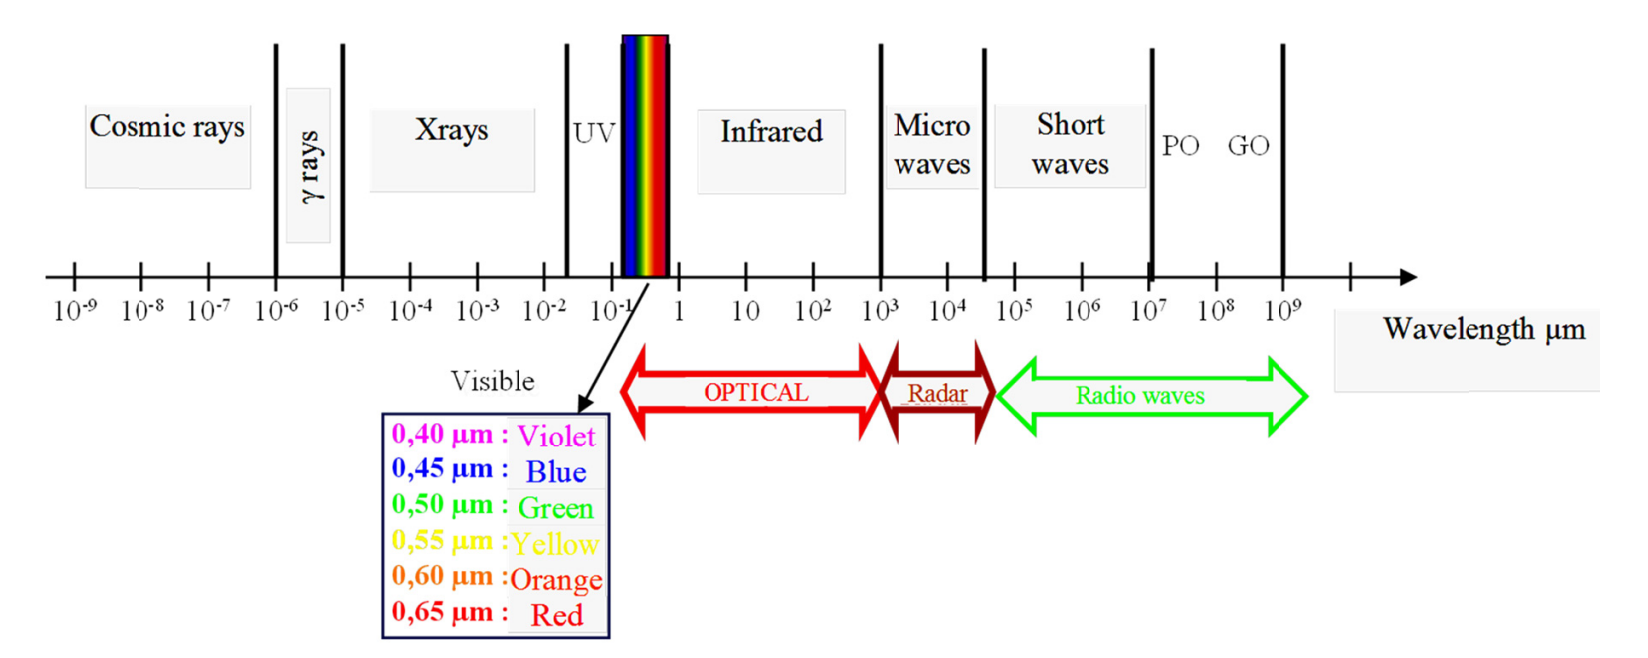
\includegraphics[width=\textwidth]{Figures/C2/espectro.png} % Cambia 'imagen.svg' al nombre de tu archivo SVG
%     \caption{Espectro electromagnético (falta formatear y referenciar). Tomado de \cite{BaghdadiOpticalMethods}.}
%     \label{fig:imagen}
% \end{figure}

% \section{Interacción radiación-materia}

% Esta sección esta destinada a describir físicamente las definiciones y conceptos esenciales para comprende la señal medida con un instrumento óptico. El área de la ciencia que mide la radiación es llamada radiometría. La transferencia radiativa describe interacción radiación-materia. La radiación puede ser modelada como una onda que se propaga por el espacio con determinadas características como: su longitud de onda, su velocidad de propagación, su intensidad, su fase y su estado de polarización.

% En teledetección, cada rango del espectro tiene aplicaciones específicas basadas en su interacción con la atmósfera y la superficie terrestre. Por ejemplo, las ondas de radio son útiles para penetrar nubes y capturar imágenes independientemente de la luz solar, mientras que las imágenes en el espectro visible proporcionan una representación cercana a lo que percibe el ojo humano.


% La radiación en diferentes partes del espectro electromagnético tiene propiedades únicas. Las radiaciones más energéticas, como los rayos X y los rayos gamma, tienen longitudes de onda cortas y alta frecuencia, lo que les permite penetrar a través de materiales sólidos, una propiedad utilizada en aplicaciones médicas y de seguridad. En contraste, las ondas de radio tienen longitudes de onda más largas y frecuencias más bajas, adecuadas para la comunicación a larga distancia.



% \subsection{Propiedades radiativas de la materia}

% \subsubsection{Noción de reflectancia}
% La reflectancia se define como la proporción de la radiación electromagnética que es reflejada por una superficie en comparación con la que incide sobre ella. Este coeficiente es crucial para entender cómo diversas superficies absorben y reflejan la energía solar en distintas longitudes de onda del espectro electromagnético.

% Cuando la radiación incide en una superficie, parte de esta energía es reflejada, otra absorbida, y una fracción transmitida. La cantidad reflejada depende de las propiedades del material y de la longitud de onda de la radiación incidente. Matemáticamente, la reflectancia (\(R\)) se expresa como:

% \begin{equation}
%     R(\lambda) = \frac{I_r(\lambda)}{I_i(\lambda)}
% \end{equation}

% donde \(I_r(\lambda)\) es la intensidad de la radiación reflejada e \(I_i(\lambda)\) es la intensidad de la radiación incidente, ambas en la longitud de onda \(\lambda\).

% La reflectancia de una superficie puede variar con la dirección e incluye dependencias de la geometría de iluminación y observación. En teledetección, se usa el concepto de reflectancia bidireccional para analizar cómo varía la reflectancia con los ángulos de iluminación y observación.

% Además, la reflectancia es fundamental para modelar el albedo de la Tierra, esencial en estudios sobre el balance energético y el cambio climático.

% En teledetección, se utiliza para caracterizar y clasificar diferentes tipos de coberturas terrestres mediante sus firmas espectrales. Por ejemplo, la vegetación sana muestra mayor reflectancia en el infrarrojo cercano y menor en el rojo visible, lo que es la base para índices de vegetación como el NDVI.

% La calibración radiométrica de los sensores y la corrección de los efectos atmosféricos son esenciales para obtener mediciones precisas de reflectancia, lo que permite comparar datos a lo largo del tiempo y del espacio.

% \begin{figure}[htbp]
%     \centering
%     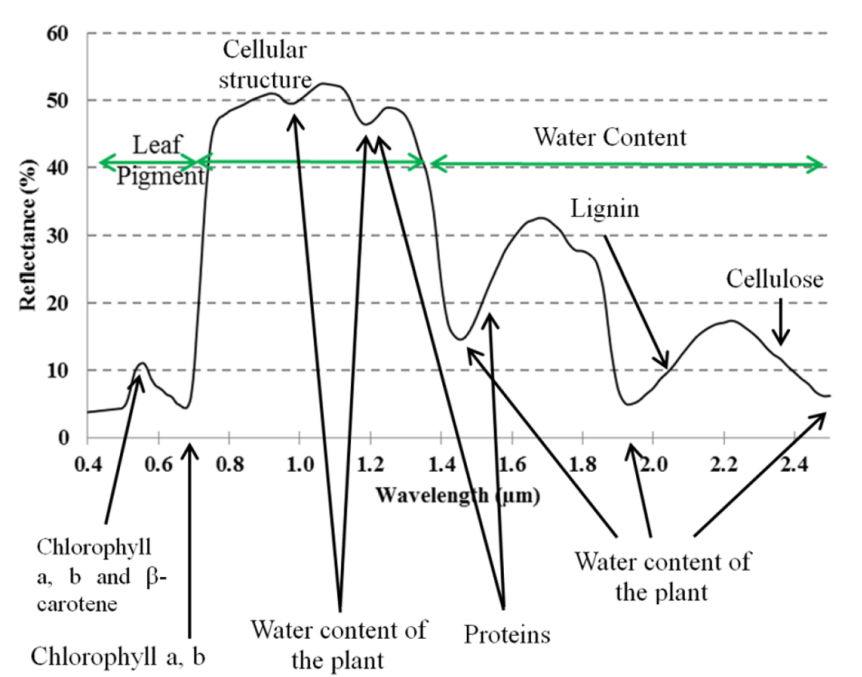
\includegraphics[width=0.7\textwidth]{Figures/C2/reflectancia.png}
%     \caption{Reflectancia de múltiples objetos. Tomado de \cite{BaghdadiOpticalMethods}.}
%     \label{fig:refl}
% \end{figure}

% \subsubsection{Noción de absorbancia}

% La absorbancia mide la cantidad de luz que una muestra absorbe al pasar a través de ella. Se define como el logaritmo negativo de la transmitancia (\(T\)):

% \begin{equation}
%     A = -\log_{10}(T) = -\log_{10}\left(\frac{I}{I_0}\right)
% \end{equation}

% donde \(I\) es la intensidad de la luz transmitida y \(I_0\) la intensidad de la luz incidente. La relación entre el coeficiente de absorción (\(\alpha\)) y la absorbancia en un medio homogéneo se describe mediante la ley de Beer-Lambert:

% \begin{equation}
%     A = \alpha \cdot l \cdot c
% \end{equation}

% donde \(l\) es la longitud del camino óptico y \(c\) la concentración del absorbente. Esta propiedad es vital para el análisis en teledetección y otras aplicaciones, desde el monitoreo de la calidad del agua hasta la evaluación de la salud vegetal.

% \subsubsection{Noción de transmitancia}
% La transmitancia indica la proporción de luz que atraviesa una sustancia respecto a la luz incidente, definida como:

% \begin{equation}
%     T = \frac{I}{I_0}
% \end{equation}

% Está inversamente relacionada con la absorbancia, y su estudio es crucial en teledetección para modelar y corregir los efectos atmosféricos en imágenes de satélite, mejorando la precisión de las observaciones de la superficie terrestre.

% \subsubsection{Noción de difusión}


% \section{Imagen (Cambiar por procesamiento de imagenes)}



% \begin{enumerate}
%     \item 
% \end{enumerate}

% \subsection{Concepto de imágen}
% \subsection{Sistemas fromadores de imágenes}



% \begin{figure}[htbp]
%     \centering
%     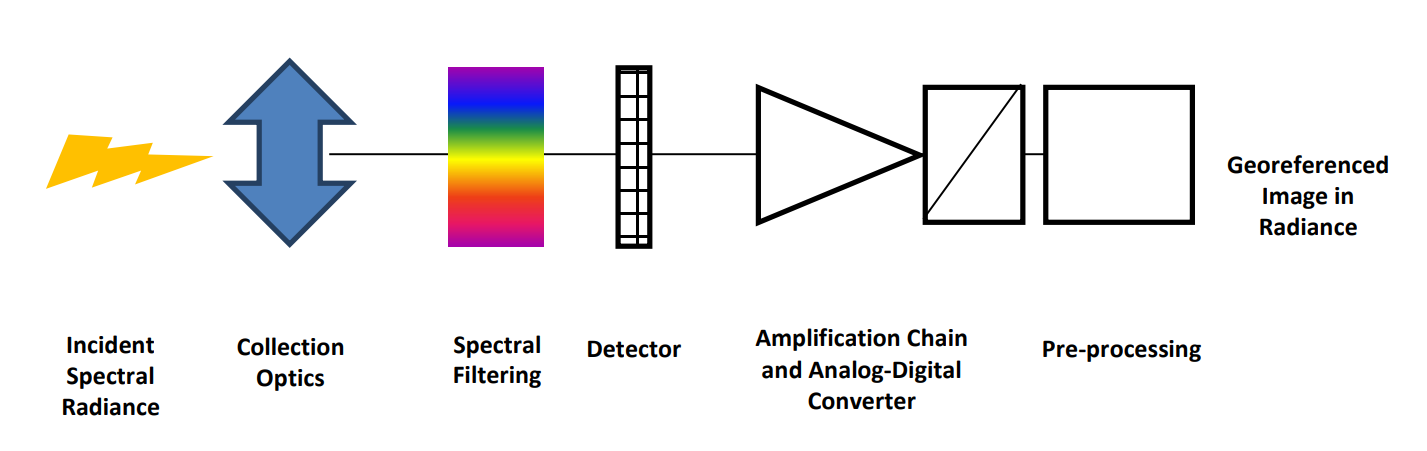
\includegraphics[width=0.9\textwidth]{Figures/C2/esquea_sis_imagen.png}
%     \caption{Esquema de un sistema formador de imagen. Tomado de \cite{BaghdadiOpticalMethods}.}
%     \label{fig:esq_sis_ima}
% \end{figure}

% \subsection{Sensores ópticos}


% %% Al-Hourani2023LinePlatforms
% El uso de cámaras multiespectrales montadas en plataformas UAV (vehículos aéreos no tripulados) se ha vuelto cada vez más común en el monitoreo agrícola y ambiental. Estas tecnologías permiten la evaluación precisa de la vegetación mediante la captura de información espectral detallada que puede ser utilizada para calcular índices de vegetación como el NDVI (Índice de Vegetación de Diferencia Normalizada). Este estado del arte revisa los principios de operación y el diseño de cámaras multiespectrales, con un enfoque en el artículo “Line Scan Hyperspectral Imaging Framework for Open Applications”.

% \subsubsection{Principios Matemáticos del Sistema de Imágenes Hiperespectrales}
% El sistema de imágenes hiperespectrales propuesto en el artículo utiliza un enfoque de escaneo en línea (line-scan), también conocido como escaneo de empuje (push broom), donde la escena se escanea línea por línea. La imagen hiperespectral resultante es un cubo de datos 3D $H(x, y, \lambda)$, con dos dimensiones representando características espaciales ($x$, $y$) y la tercera dimensión representando la información espectral $\lambda$ \cite{line_scan_hyperspectral}.

% Matemáticamente, cada línea escaneada es dispersada espectralmente usando un sistema de lentes y un espectroscopio, proyectando un espectro sobre un sensor CMOS. La intensidad de la imagen monocromática para un píxel en particular se calcula mediante:

% \[
% \tilde{I}_{\text{mono}}(x, y) = f \left( A \cdot T \cdot \int_{\lambda_{\text{min}}}^{\lambda_{\text{max}}} g(\lambda) \cdot s(\lambda) \, d\lambda \right)
% \]

% donde $A$ es el área del sensor, $T$ es el tiempo de exposición, $g(\lambda)$ es la irradiancia espectral, y $s(\lambda)$ es la sensibilidad espectral del sensor \cite{line_scan_hyperspectral}.

% \subsubsection{Diseño del Sistema de Cámaras Multiespectrales}
% El diseño del sistema multiespectral descrito en el artículo se enfoca en utilizar componentes accesibles y de bajo costo para construir una plataforma asequible. La plataforma incluye un sistema optomecánico que emplea espejos de galvanómetro para escanear la escena en un eje, mientras que una lente de montaje CS y un espectroscopio sencillo permiten la captura de imágenes espectrales \cite{Al-Hourani2023LinePlatforms}.

% El sistema diseñado fue evaluado comparando los resultados espectrales con mediciones realizadas por espectrómetros comerciales de gama alta, mostrando una precisión espectral comparable a pesar del bajo costo de los componentes utilizados. La metodología de escaneo en línea permitió capturar datos espectrales con alta resolución espacial y espectral, cruciales para la determinación precisa de índices de vegetación \cite{Al-Hourani2023LinePlatforms}.

% La integración de cámaras multiespectrales en UAVs para el monitoreo de la vegetación es una herramienta poderosa para la agricultura de precisión. Los desarrollos presentados en el artículo demuestran que es posible construir sistemas eficientes y de bajo costo que puedan capturar información espectral detallada, lo que facilita la evaluación precisa de la salud de los cultivos mediante la determinación de índices de vegetación.

% Estos avances en la tecnología de imágenes hiperespectrales y su aplicación en UAVs prometen mejorar significativamente las prácticas agrícolas y el monitoreo ambiental, proporcionando datos críticos para la toma de decisiones informada.

% \subsection{Óptica de Imágenes para sistemas hiperespectrales (HSI)}

% En la teledetección y, particularmente, en el estudio de índices de vegetación, la imagen hiperespectral (HSI) es una herramienta poderosa para capturar información detallada sobre la composición espectral de la vegetación y otros objetos en la Tierra. La imagen HSI se representa como un cubo de datos tridimensional que incluye dos dimensiones espaciales y una tercera dimensión que captura la información espectral. Este cubo se conoce como "cubo hiperespectral" \cite{Al-Hourani2023LinePlatforms}.

% Existen varios métodos para adquirir este cubo de datos 3D:

% \begin{enumerate}
%     \item \textbf{Escaneo puntual (whiskbroom)}: Este método escanea individualmente cada punto de la escena y obtiene la información espectral para cada píxel [x, y]. Aunque proporciona una alta resolución espectral, su proceso es lento debido a la necesidad de capturar punto por punto.

%     \item \textbf{Escaneo de banda espectral (framing)}: En este método, la imagen proyectada pasa a través de filtros de banda pasante sintonizables, que permiten solo una parte estrecha del espectro a la vez. Luego, el filtro se desplaza a través del espectro. A pesar de ser más rápido que el método whiskbroom, requiere filtros costosos que ofrezcan velocidad y precisión.

%     \item \textbf{Método de instantánea (snapshot)}: Aquí, la escena se duplica ópticamente en múltiples réplicas pequeñas, y cada réplica pasa por un filtro de banda estrecha. Este método permite una adquisición más rápida y es conocido como "método de instantánea". Sin embargo, requiere sistemas ópticos microfabricados especializados, lo cual puede ser costoso y técnicamente complejo.

%     \item \textbf{Escaneo lineal (push broom)}: Este método, adoptado en muchas aplicaciones de HSI debido a su eficiencia, escanea la escena línea por línea. Cada línea escaneada se extiende en una imagen espatio-espectral 2D [y, z], y estas imágenes se apilan para formar el cubo de datos hiperespectrales [x, y, z]. 
% \end{enumerate}

% En este método, se emplea un espectrógrafo típico que dispersa la luz de la línea escaneada, convirtiéndola en una imagen espatio-espectral 2D. El proceso implica usar una lente de imagen que forma una imagen real del objetivo en una rendija estrecha, seguida de lentes colimadoras para dirigir la luz colimada hacia ópticas dispersivas, como un prisma óptico o una red de difracción.

% \begin{itemize}
%     \item \textbf{Prismas ópticos}: Ofrecen bajas pérdidas de transmisión pero presentan una dispersión espectral no lineal, lo que requiere una cuidadosa calibración.

%     \item \textbf{Redes de difracción}: Dispersan la luz de manera lineal, lo que simplifica la calibración. La configuración típica es un sistema prismático donde la red de difracción se encuentra entre dos prismas, asegurando que la entrada y salida de la luz estén alineadas.
% \end{itemize}

% \subsection{Aplicación de Sensores}

% Una vez dispersada la luz en sus componentes espectrales, un sensor óptico, como un sensor CMOS (Complementary Metal-Oxide-Semiconductor), captura la imagen espatio-espectral. Aunque los sensores CMOS tienen ciertas limitaciones en términos de ruido y rango de longitud de onda (particularmente en el infrarrojo cercano), su velocidad de lectura y bajo costo los hacen adecuados para muchas aplicaciones de teledetección. En casos donde se requieren rangos de longitud de onda más allá del infrarrojo cercano, materiales especializados como el telururo de cadmio de mercurio (MCT) pueden ser utilizados, aunque a un costo más elevado.

% \subsection{Relevancia para la Teledetección y los Índices de Vegetación}

% La capacidad de capturar información espectral detallada permite que los sistemas de imágenes hiperespectrales sean utilizados para calcular índices de vegetación con precisión, proporcionando datos cruciales para la evaluación de la salud de las plantas, el monitoreo del estrés hídrico, y la gestión de recursos agrícolas. Estos métodos ópticos y el uso de sensores avanzados en la adquisición de imágenes multiespectrales son fundamentales para aplicaciones precisas de agricultura y monitoreo ambiental.



% \section{Índices de vegetación}

% En la investigación ambiental, los cocientes de bandas son frecuentemente utilizados como índices de vegetación con el fin de cuantificar la cantidad de vegetación que puede aparecer en una imagen digital multiespectral \cite{Vaiopoulos2004TheIndices}. La relación matemática general de un índice de vegetación, $R$, formado por el cociente de bandas, puede escribirse como:

% \begin{equation}
% R = \frac{a_1x + a_2y + a_3}{b_1x + b_2y + b_3}
% \end{equation}

% donde $x$ e $y$ son los valores de brillo de los píxeles (o valores de reflectancia) en la banda del infrarrojo cercano (NIR) y la banda roja, respectivamente. Los coeficientes $a_1, a_2, a_3, b_1, b_2$ y $b_3$ son definidos usualmente por criterios empíricos para mejorar la sensibilidad del índice de vegetación a diferentes tipos de cobertura terrestre \cite{Vaiopoulos2004TheIndices}.

% En algunos casos, en lugar de $R$, se utiliza una función de $R$ (como la raíz cuadrada de $R$ o $R$ multiplicado por una constante) para definir el índice de vegetación.

% \begin{equation}
% \text{SVI} = \frac{x}{y}
% \end{equation}

% Este índice de vegetación conocido como Simple Ratio Index (SVI) utiliza el cociente entre las reflectancias en el infrarrojo cercano y el rojo, proporcionando una medida simple de la cantidad de vegetación en la escena \cite{Vaiopoulos2004TheIndices}.


% %% Myneni1995TheIndexes

% El uso de índices espectrales de vegetación en la teledetección ha permitido importantes avances en la monitorización y cuantificación de la vegetación a nivel global. Myneni et al. (1995) en su artículo \textit{The Interpretation of Spectral Vegetation Indexes} \cite{Myneni1995TheIndexes}, destacan que los índices espectrales de vegetación pueden correlacionarse con parámetros clave como el área foliar, la biomasa y el funcionamiento fisiológico de la vegetación.

% Los índices de vegetación se clasifican en tres tipos principales:


% \subsection{Tipo I: Índices Lineales}
% Un ejemplo común de índices lineales es el Índice de Vegetación de Diferencia Normalizada (NDVI), que mide el contraste entre la reflectancia en el rojo (absorción por la clorofila) y el infrarrojo cercano (reflejado por la estructura celular de las hojas).

% \begin{equation}
%     \text{NDVI} = \frac{(NIR - Red)}{(NIR + Red)}
% \end{equation}

% Donde:
% \begin{itemize}
%     \item $NIR$: Reflectancia en el infrarrojo cercano (0.75-1.35 µm).
%     \item $Red$: Reflectancia en la banda del rojo (0.6-0.7 µm).
% \end{itemize}

% \subsection{Tipo II: Índices No Lineales}
% Este tipo de índices utiliza productos de reflectancia para minimizar efectos atmosféricos. Un ejemplo es el Índice de Monitoreo del Medio Ambiente Global (GEMI), que se expresa de la siguiente manera:

% \begin{equation}
%     \eta = \frac{2 \cdot (NIR^2 - Red^2)}{NIR + Red + 0.5}
% \end{equation}

% \begin{equation}
%     \text{GEMI} = \eta \cdot (1 - 0.25 \cdot \eta) - \frac{(Red - 0.125)}{1 - Red}
% \end{equation}

% \subsection{Tipo III: Índices Derivados de Segunda Orden}
% Estos índices corrigen los efectos atmosféricos y del suelo. El Índice de Vegetación Atmosféricamente Resistente (ARVI) usa bandas adicionales como la del azul para realizar estas correcciones:

% \begin{equation}
%     \text{ARVI} = \frac{(NIR - (2 \cdot Red - Blue))}{(NIR + (2 \cdot Red + Blue))}
% \end{equation}

% Donde:
% \begin{itemize}
%     \item $Blue$: Reflectancia en la banda del azul (alrededor de 0.45 µm).
% \end{itemize}

% Los autores \cite{Myneni1995TheIndexes} concluyen que los índices espectrales de vegetación son indicadores fiables de la abundancia de clorofila y la absorción de energía por la vegetación. Esto permite su aplicación en estudios a gran escala, como el monitoreo del crecimiento de cultivos y la evaluación de la fracción de radiación fotosintéticamente activa absorbida. Además, estos índices se saturan en altas concentraciones de biomasa, lo que puede limitar su aplicabilidad en ecosistemas muy densos.

% Este trabajo establece una base teórica sólida para la teledetección espectral de la vegetación, al correlacionar las características ópticas de la vegetación con los índices derivados de la reflectancia espectral, facilitando así aplicaciones en estudios globales de la biosfera terrestre.

% \section{Teledetección de índices de vegetación mediante imágenes}



% %% Bazrafkan et al. (2023)
% Bazrafkan et al. (2023) evaluaron cinco algoritmos de aprendizaje automático para predecir la madurez de los guisantes secos en parcelas de campo, utilizando datos recopilados por UAS. Los algoritmos consideraron una variedad de variables, incluyendo métricas de altura de cultivos, bandas espectrales estrechas y 18 índices de vegetación de color y espectrales distintos. La eliminación hacia atrás de características se utilizó para optimizar el rendimiento predictivo del modelo \cite{Bazrafkan2023PredictingUASs}.
% El estudio reveló que el enfoque más efectivo para evaluar la madurez de los guisantes secos involucraba una combinación de bandas espectrales estrechas, borde rojo, NIR, y índices de vegetación basados en RGB, junto con métricas de textura de imágenes y métricas de altura de cultivos. La implementación de un modelo de bosque aleatorio mejoró aún más la precisión de los resultados, mostrando el mayor nivel de precisión con un valor de 0.99 para las tres métricas de precisión, recall y puntajes f1 \cite{Bazrafkan2023PredictingUASs}.

% %% Deng et al. (2018)
% La metodología aplicada por Deng et al. (2018) incluyó un flujo de trabajo detallado para el procesamiento de imágenes de Mini-MCA6, que comprendió la corrección de ruido, corrección de viñeteo, alineación de banda a banda, y calibración radiométrica utilizando métodos como el lineal empírico (EL) y la línea empírica de subbanda (SEL). Este enfoque meticuloso permitió generar ortomosaicos georreferenciados de seis bandas con alta precisión \cite{Deng2018UAV-basedCameras}.
% Deng et al. (2018) observaron que la precisión de los valores de reflectancia de la cámara Mini-MCA6 era superior a la de la cámara Sequoia, particularmente cuando se utilizaba el método de calibración adecuado. En términos de predicción de valores SPAD, el reNDVI mostró un mejor desempeño que el NDVI en todas las condiciones de tratamiento de nitrógeno, independientemente de la cámara utilizada. Este hallazgo subraya la relevancia del reNDVI para evaluar el estado nutricional de los cultivos, especialmente en condiciones de campo variadas \cite{Deng2018UAV-basedCameras}.


% %% Vuletić et al
% El estudio realizado por Vuletić et al. se centra en la imagen multiespectral de corto alcance utilizando un sistema MS-D. Este sistema emplea cámaras multiespectrales calibradas con respecto a una cámara RGB-D para la inscripción precisa de imágenes, esencial para el monitoreo y la evaluación de la salud de los cultivos mediante índices de vegetación \cite{Vuletic2023Close-rangeSystem}. El sistema MS-D demostró superioridad sobre los métodos basados en características tradicionales en diversas pruebas, incluyendo la inscripción de imágenes en entornos reales y simulados. Esto se traduce en una mayor precisión para la evaluación del estrés hídrico en plantas, mostrando cambios significativos en índices como NDVI y NDRE en condiciones controladas de estrés por riego \cite{Vuletic2023Close-rangeSystem}. El sistema MS-D se presenta como una herramienta robusta, rápida y precisa, adecuada para el monitoreo de plantas sin la necesidad de recalibración entre usos, facilitando su aplicación en entornos agrícolas variados \cite{Vuletic2023Close-rangeSystem}.

% % Smeesters2023Wide-Field-of-ViewMonitoring
% El diseño de cámaras multiespectrales de amplio campo de visión para la monitorización continua del césped se aborda mediante un sistema de cinco canales que cubre las bandas del visible, infrarrojo cercano y térmico. Se optimiza el diseño de la cámara para un amplio campo de visión, permitiendo la integración en dispositivos de iluminación y la evaluación autónoma y continua del estrés hídrico y la presencia de enfermedades o plagas en las plantas \cite{Smeesters2023Wide-Field-of-ViewMonitoring}. Los resultados demuestran una calidad de imagen excepcional en todos los canales de imagen, confirmada por una función de transferencia de modulación (MTF) que supera un contraste de 0.5 en una frecuencia espacial de 72 líneas por milímetro para los diseños de imagen visible e infrarroja cercana. Este sistema propuesto supera las limitaciones de los sistemas tradicionales montados en UAVs, que suelen tener un campo de visión reducido \cite{Smeesters2023Wide-Field-of-ViewMonitoring}. El estudio concluye que el diseño de la cámara multispectral de campo visual amplio es viable para el monitoreo automatizado y continuo de campos de césped, optimizando el uso de recursos y minimizando la necesidad de intervenciones manuales frecuentes. Esta tecnología podría adaptarse para una variedad de aplicaciones agrícolas donde el monitoreo continuo es crucial \cite{Smeesters2023Wide-Field-of-ViewMonitoring}.

% % Silva et al.
% Silva et al. \cite{Orlando2023POTENTIALIRRIGATION} investigan la monitorización de la irrigación de cultivos de café utilizando imágenes multiespectrales obtenidas por sensores incorporados en vehículos aéreos no tripulados (UAV). El estudio evalúa la capacidad de cámaras de bajo costo para discriminar diferentes tratamientos de agua en el cultivo de café, utilizando el Potencial Hídrico Foliar (LWP) como indicador. La metodología consiste en la captura de imágenes multiespectrales a través de un UAV equipado con una cámara Mapir Survey3W. La cámara capta bandas del espectro visible, NIR y red. La evaluación del LWP se realiza in situ, utilizando una cámara de presión de Scholander para medir el potencial hídrico de las hojas del café durante diferentes etapas del ciclo de irrigación. Se emplean técnicas de aprendizaje automático para modelar y predecir el LWP a partir de los índices de vegetación derivados de las imágenes \cite{Orlando2023POTENTIALIRRIGATION}. Los resultados demuestran que el índice de vegetación NDVI, derivado de las imágenes multiespectrales, permite una discriminación efectiva de los diferentes regímenes de riego aplicados. El modelo de árbol aleatorio y el algoritmo SMOreg destacan por su capacidad para predecir el LWP con un bajo error cuadrático medio (RMSE), lo que indica un alto grado de precisión en la detección del estrés hídrico en el cultivo de café \cite{Orlando2023POTENTIALIRRIGATION}. El estudio concluye que las imágenes multiespectrales capturadas por UAVs, combinadas con técnicas avanzadas de procesamiento de datos y aprendizaje automático, ofrecen una metodología prometedora para la monitorización precisa y en tiempo real de la irrigación en cultivos de café. Esta tecnología tiene el potencial de mejorar la gestión del agua en la agricultura, optimizando el uso de recursos y aumentando la sostenibilidad de las prácticas agrícolas \cite{Orlando2023POTENTIALIRRIGATION}.

% % Goebel e Iwaszczuk Goebel2023SPECTRALCAMERA
% Goebel e Iwaszczuk \cite{Goebel2023SPECTRALCAMERA} presentan un estudio que utiliza una cámara de corto alcance para la observación de plantas bajo condiciones de estrés, explorando la utilidad de distintos índices de vegetación a partir de imágenes multiespectrales. El estudio utiliza el sistema de cámara MicaSense RedEdge MX Dual en configuraciones de corto alcance para monitorear plantas interiores y en sotobosque, analizando cambios en la reflectancia de las hojas bajo estrés por falta de agua o luz solar. Se emplean índices de vegetación como NDVI y NDRE para evaluar el estado de salud de las plantas, utilizando algoritmos de fusión y registro de imágenes para correlacionar los datos de múltiples bandas espectrales \cite{Goebel2023SPECTRALCAMERA}. Los resultados muestran que los índices de vegetación, especialmente NDVI y NDRE, son efectivos para detectar estrés en las plantas, indicando diferencias significativas en la reflectancia de las bandas del rojo y el borde rojo entre plantas saludables y estresadas. La comparación de estos índices a lo largo del tiempo permite identificar los cambios en la salud vegetal y ajustar las intervenciones de manejo de manera más efectiva \cite{Goebel2023SPECTRALCAMERA}. El estudio concluye que el uso de cámaras multiespectrales en configuraciones de corto alcance es una herramienta valiosa para la detección precoz del estrés vegetal y puede integrarse en estrategias de manejo para mejorar la respuesta a condiciones ambientales adversas. Además, sugieren la necesidad de mejorar la calibración y el registro de imágenes para optimizar la calidad de los datos espectrales recogidos \cite{Goebel2023SPECTRALCAMERA}.



% % Villacres2022ConstructionAreas
% \cite{Villacres2022ConstructionAreas}, se investiga la construcción de mapas tridimensionales de índices de vegetación (VI) obtenidos de imágenes multiespectrales de UAV en áreas forestadas. La metodología incorpora la generación de un punto de nube, la segmentación del dosel y la estimación de VI mediante el uso de regresores de proceso gaussiano (GPR). El estudio utiliza imágenes multiespectrales capturadas por una cámara montada en un vehículo aéreo no tripulado (UAV) para crear un punto de nube, en el que se estiman los VI en los puntos que pertenecen al dosel del bosque. Se investiga una combinación de filtrado de puntos de suelo y umbralización de VI para clasificar los puntos del dosel. Los regresores GPR, junto con el bosque aleatorio (RF) y la regresión de cresta kernel (KRR), se investigan para estimar doce VIs relacionados con el contenido de humedad del combustible (FMC) \cite{Villacres2022ConstructionAreas}. Los resultados muestran que la combinación de filtrado de suelo y umbralización de VI para la segmentación de puntos del dosel logra una precisión de hasta 93.27\%, y el uso de GPR logra recuperar once de los doce VIs con un error cuadrático medio de raíz (RMSE) de 0.175 y un coeficiente de determinación de 0.18. Estos métodos superan al RF y KRR en precisión y capacidad de recuperación de VI \cite{Villacres2022ConstructionAreas}. El estudio concluye que los mapas de VI basados en imágenes multiespectrales de UAV proporcionan una metodología robusta para la monitorización precisa del FMC en áreas forestadas. Esta técnica permite mejorar las estrategias de manejo forestal y la planificación de la respuesta a incendios \cite{Villacres2022ConstructionAreas}.



% % Kim2023DeepClassification
% En el estudio de Kim et al. \cite{Kim2023DeepClassification}, se explora el uso de imágenes multiespectrales y un índice de vegetación para clasificar terrenos agrícolas mediante aprendizaje profundo. Este estudio propone un método para la adquisición y preprocesamiento de imágenes multiespectrales mediante drones para optimizar la clasificación de terrenos agrícolas. Se utilizan técnicas de aprendizaje profundo para comparar el rendimiento de los conjuntos de datos de entrada que incluyen diferentes bandas espectrales y el índice de vegetación NDVI, obtenidos mediante cámaras multispectrales \cite{Kim2023DeepClassification}. Los resultados indican que la inclusión de bandas del borde rojo y NIR junto con datos RGB mejora significativamente la precisión de la clasificación de terrenos agrícolas. El índice de vegetación NDVI, cuando se usa en combinación con estas bandas, no mejora la precisión de la clasificación, lo que sugiere que la información espectral específica es más relevante para las tareas de clasificación en este contexto \cite{Kim2023DeepClassification}. Se concluye que la optimización de los conjuntos de datos de entrada para el aprendizaje profundo es crucial para mejorar la eficiencia y precisión de la clasificación de terrenos agrícolas. El estudio destaca la importancia de seleccionar adecuadamente las bandas espectrales para la inclusión en los modelos de aprendizaje profundo, basado en las características específicas de las plantas y las condiciones del terreno \cite{Kim2023DeepClassification}.


% % Fuentes-Peailillo2018ComparisonUAV
% Fuentes-Peñailillo et al. \cite{Fuentes-Peailillo2018ComparisonUAV} comparan índices de vegetación obtenidos mediante sensores RGB y multiespectrales colocados en UAVs para identificar vegetación y suelo, destacando las ventajas de los UAVs para obtener datos con mayor resolución espacial, espectral y temporal. El estudio utiliza dos UAVs para capturar imágenes RGB y multiespectrales de un viñedo. Se comparan cuatro índices derivados de las imágenes RGB con el índice de vegetación normalizado (NDVI) obtenido de un sensor multiespectral. La metodología incluye la creación de mapas de clases de NDVI y su comparación con los índices RGB mediante un conteo de píxeles \cite{Fuentes-Peailillo2018ComparisonUAV}. Los índices RGB, particularmente el Índice de Verdor Triangular (TGI), mostraron patrones espaciales similares al NDVI, aunque la identificación visual de vegetación presentó errores. Esto sugiere que mientras los índices RGB pueden replicar los patrones del NDVI, la precisión en la clasificación de vegetación y suelo es limitada sin técnicas de clasificación más complejas \cite{Fuentes-Peailillo2018ComparisonUAV}. El estudio concluye que los sensores RGB, a pesar de ser menos costosos, requieren métodos avanzados de procesamiento de datos para igualar la precisión de los sensores multiespectrales en aplicaciones de agricultura de precisión. Se recomienda el uso de sensores multiespectrales para aplicaciones que requieran alta precisión en la segmentación de imágenes \cite{Fuentes-Peailillo2018ComparisonUAV}.


% % Garcia2019NDVI
% En el estudio de García Cárdenas et al. \cite{Garcia2019NDVI}, se analizaron las dinámicas de dos índices de vegetación, el \textit{Normalized Difference Vegetation Index} (NDVI) y su variante que utiliza la banda verde, el \textit{Green Normalized Difference Vegetation Index} (GNDVI), en un cultivo de arroz de la variedad Fedearroz 2000 en fase de reproducción. Estos índices fueron calculados mediante geoprocesamiento de imágenes multiespectrales capturadas por drones (UAVs) con el fin de identificar zonas de estrés, vegetación saludable o densa. El área de estudio fue una parcela de arroz de 4.1 hectáreas, ubicada en el departamento de Norte de Santander, Colombia. Se llevaron a cabo dos vuelos, uno al inicio de la fase de reproducción (4 de septiembre de 2016) y otro al final de esta fase (8 de octubre de 2016).

% Las imágenes fueron capturadas con una cámara Canon S100 equipada con un filtro NGB (infrarrojo cercano, verde y azul), lo que permitió la creación de mosaicos ortofotográficos para ambos vuelos. Se observó un incremento en los valores de NDVI entre ambos vuelos, lo que refleja el crecimiento del cultivo durante esta fase crítica, caracterizada por la elongación del tallo y el desarrollo de la panícula. Este incremento coincidió con estudios previos que correlacionan el NDVI con el rendimiento del arroz durante la fase de reproducción \cite{Garcia2019NDVI}.

% Este estudio demostró la capacidad de los UAVs equipados con cámaras multiespectrales para capturar imágenes con alta resolución espacial y espectral, permitiendo a los agricultores tomar decisiones precisas sobre el manejo de cultivos, como la identificación de zonas con deficiencias nutricionales y la optimización del uso de fertilizantes y agua. Además, se destacó la utilidad del GNDVI, que mostró ser más sensible a la concentración de clorofila que el NDVI, lo que permite una mejor detección de zonas bajo estrés en etapas tempranas del crecimiento del cultivo.

% % Tello2021Contaminacion
% Tello-Cifuentes y Díaz-Paz \cite{Tello2021Contaminacion} presentaron un análisis de la contaminación ambiental en Medellín, Colombia, utilizando imágenes Landsat y técnicas de teledetección, aplicando índices de vegetación y otras métricas ambientales. El estudio incluyó el cálculo del NDVI, TSAVI (Índice de Vegetación Ajustado al Suelo Transformado) y el NDWI (Índice de Diferencia Normalizada del Agua), en combinación con variables de calidad del aire, como el material particulado (PM10 y PM2.5) y los niveles de dióxido de nitrógeno (NO2) y ozono (O3).

% Mediante la integración de estos índices y técnicas de análisis de componentes principales (PCA), los autores lograron identificar las áreas más afectadas por la contaminación en Medellín. Se encontró que las zonas con menor cobertura vegetal y mayor densidad de construcciones presentaban los mayores niveles de contaminación, mientras que las áreas con mayor vegetación mostraron mejor calidad del aire. Este tipo de estudios demuestra la relevancia de los índices de vegetación en el monitoreo ambiental, no solo en el contexto agrícola, sino también en la gestión de la calidad del aire y la planificación urbana en ciudades como Medellín.

% Los resultados de este estudio subrayan la importancia de la vegetación en la mitigación de la contaminación ambiental y proporcionan una metodología sólida para la toma de decisiones en la planificación urbana, utilizando técnicas de teledetección para identificar rápidamente áreas críticas que requieren intervención \cite{Tello2021Contaminacion}.

% \subsection{Caracterización espectral y monitoreo de bosques de manglar}

% En el litoral Pacífico colombiano, se ha estudiado el uso de imágenes de satélite para la caracterización y monitoreo de los bosques de manglar, aplicando índices de vegetación como el NDVI (Normalized Difference Vegetation Index), el SAVI (Soil Adjusted Vegetation Index) y el CMRI (Combined Mangrove Recognition Index). Estas herramientas permiten la evaluación de la salud y densidad de los manglares a lo largo del tiempo y bajo diferentes condiciones mareales. Un estudio reciente aplicó estos índices utilizando imágenes de los satélites Landsat 5, 7 y 8, para monitorizar el comportamiento espectral de los manglares en diferentes momentos entre 1998 y 2017, observándose aumentos en los valores del NDVI y SAVI, lo que indica un buen estado fotosintético de los BM durante este período .

% % Tello2021Contaminacion
% La investigación destaca que, debido a la interacción de los manglares con la marea, el comportamiento de los índices de vegetación varía, especialmente en zonas costeras con una alta influencia mareal. La firma espectral de los manglares tiende a subestimarse en imágenes capturadas en pleamar, lo que afecta los valores obtenidos para los índices de vegetación, como el NDVI y el CMRI. Por esta razón, es crucial realizar un análisis espacio-temporal que considere múltiples momentos mareales para evitar interpretaciones erróneas de la densidad y salud de los manglares .

% El estudio concluye que la aplicación del CMRI, un índice diseñado específicamente para manglares, resultó ser particularmente útil en la identificación de estas áreas. Este índice combina la información del NDVI y el NDWI (Normalized Difference Water Index), permitiendo una evaluación más precisa de los manglares en condiciones de alta humedad y marea .

% % PereaArdila2021
% La teledetección ha sido ampliamente utilizada en la caracterización y monitoreo de diferentes ecosistemas, incluidas áreas de manglares. En el litoral pacífico colombiano, el estudio de Perea-Ardila et al. (2021) se centró en la caracterización espectral y monitoreo de bosques de manglar (BM) en la región de Bajo Baudó, Chocó. Se emplearon imágenes satelitales de Landsat para analizar cuatro densidades de manglares utilizando combinaciones espectrales y tres índices de vegetación (IV): el Índice de Vegetación de Diferencia Normalizada (NDVI), el Índice de Vegetación Ajustado al Suelo (SAVI), y el Índice Combinado de Reconocimiento de Manglares (CMRI). Los resultados demostraron que la mejor combinación de bandas espectrales para identificar los BM fue el infrarrojo color (NIR, rojo, verde), siendo clave el comportamiento espectral de los manglares bajo diferentes condiciones mareales.

% Durante un periodo de 19 años (1998, 2014 y 2017), se registraron variaciones de hasta un 17,9\% en la reflectancia promedio de los BM, siendo los valores de los IV proporcionales a la densidad del bosque. Sin embargo, los efectos de las mareas influyeron en los resultados, reduciendo los valores de los IV en zonas de transición tierra-agua, donde la interacción con las condiciones mareales es fuerte. Estos hallazgos aportan al desarrollo de metodologías para la caracterización espacial y monitoreo de manglares mediante teledetección en Colombia, destacando la importancia del uso de sensores remotos para la conservación de estos ecosistemas estratégicos.

% % Guevara-Bonilla2020
% El uso de drones o vehículos aéreos no tripulados (VANT’s) ha incrementado notablemente en América Latina, ofreciendo nuevas oportunidades para el monitoreo de recursos naturales. Un estudio de Guevara-Bonilla et al. (2020) proporciona una síntesis de las principales características y aplicaciones de los drones en el manejo de recursos naturales en la región. Los autores destacan que la implementación de VANT’s permite obtener imágenes de alta resolución con un bajo costo operativo, comparado con otras tecnologías de monitoreo, lo que facilita el seguimiento detallado de áreas específicas con poca interferencia atmosférica. Esto resulta particularmente útil en contextos agrícolas y forestales, donde la nubosidad y las condiciones atmosféricas adversas suelen limitar la eficacia de las imágenes satelitales [(Guevara-Bonilla et al., 2020)](https://doi.org/10.18845/tm.v33i4.4528).

% Los VANT’s son especialmente útiles en la agricultura de precisión, donde se emplean para la detección de enfermedades, gestión hídrica, fertilización y monitoreo de cosechas. Asimismo, permiten la creación de modelos tridimensionales de cultivos y estimaciones de volumen, lo que proporciona información clave para mejorar la eficiencia y sostenibilidad de los sistemas agrícolas. En el ámbito forestal, los drones se utilizan para el monitoreo de plantaciones, la evaluación de la salud de los bosques, y la identificación de especies y plagas. Su capacidad para sobrevolar zonas de difícil acceso hace que los VANT’s sean una herramienta fundamental en la planificación y manejo forestal sostenible [(Guevara-Bonilla et al., 2020)](https://doi.org/10.18845/tm.v33i4.4528).

% El estudio también destaca las aplicaciones de los drones en la gestión de desastres naturales, donde son utilizados para evaluar daños en infraestructuras y generar mapas de zonas de riesgo en tiempo real, mejorando la capacidad de respuesta ante emergencias. Además, los drones se han empleado con éxito en el monitoreo de ecosistemas acuáticos, permitiendo la estimación de caudales y el análisis de la erosión en riberas, así como en la identificación de áreas susceptibles a inundaciones y sequías [(Guevara-Bonilla et al., 2020)](https://doi.org/10.18845/tm.v33i4.4528).

% % Jiménez & Agudelo, 2015
% Jiménez y Agudelo (2015) presentan un proyecto enfocado en la validación y calibración de un sensor de alta resolución para la obtención de imágenes en el rango de infrarrojo (IR) aplicables a la agricultura de precisión. Los UAVs probados, un multirrotor y un ala fija, fueron equipados con sensores RGB y NIR para generar mapas de reflectancia y calcular índices de vegetación como el NDVI (Normalized Difference Vegetation Index). Estos índices permiten evaluar parámetros críticos como el área foliar, el estrés hídrico, la actividad fotosintética y la vigorosidad de los cultivos.

% En sus pruebas de campo en los llanos orientales de Colombia, utilizaron imágenes ortorrectificadas y mosaicos generados por software especializado, como Pix4D y ArcGIS, para calcular el NDVI y otros índices relacionados. Uno de los hallazgos más importantes fue que el uso de UAVs ofrece una solución viable y de bajo costo para la captura de imágenes de alta resolución en tiempo real, especialmente en zonas con alta nubosidad, donde las imágenes satelitales son menos eficaces. Además, resaltaron la importancia de calibrar adecuadamente los sensores y de utilizar puntos de control en tierra para mejorar la precisión geométrica de los modelos de superficie digital (DSM) generados a partir de las imágenes adquiridas.

% Este estudio concluye que los UAVs no solo proporcionan una alternativa eficiente para el monitoreo de cultivos en tiempo real, sino que también permiten la creación de modelos tridimensionales del terreno, útiles para la gestión de recursos agrícolas y la planificación de cosechas (Jiménez & Agudelo, 2015).


% % Casamitjana2020SoilMoisture
% En estudios recientes sobre teledetección, se ha destacado la importancia de las imágenes multiespectrales obtenidas mediante vehículos aéreos no tripulados (UAV) para analizar la humedad del suelo en ambientes tropicales y montañosos, particularmente en los Andes colombianos \cite{Casamitjana2020SoilMoisture}. En este contexto, Casamitjana et al. (2020) realizaron un análisis exhaustivo de la humedad del suelo en Andosoles, utilizando imágenes multiespectrales de alta resolución adquiridas por UAV en la cuenca de Las Palmas, cerca de Medellín, Colombia. Los autores aplicaron varios índices de vegetación, tales como el Índice de Vegetación de Diferencia Normalizada (NDVI), el Índice de Agua de Diferencia Normalizada (NDWI), el Índice de Vegetación Ajustado por Suelo (SAVI) y el Índice de Sequía Perpendicular (PDI), para correlacionar la humedad superficial del suelo con el uso del terreno (pasto, papa y suelo desnudo) \cite{Casamitjana2020SoilMoisture}.

% En su investigación, encontraron que los índices NDVI, NDWI y PDI se ajustaron mejor para estimar la humedad del suelo en áreas de suelo desnudo, mientras que en los cultivos de papa, el NDWI mostró la mejor correlación, independientemente de la escala de análisis. Este enfoque permitió demostrar que las imágenes multiespectrales obtenidas por UAV, con una resolución de 3 metros, son una alternativa eficaz para el análisis de la humedad del suelo en terrenos agrícolas y de pasto en ambientes montañosos tropicales, donde las imágenes satelitales tradicionales suelen ser menos útiles debido a su baja resolución espacial y las condiciones atmosféricas variables \cite{Casamitjana2020SoilMoisture}. Estos resultados son relevantes para la agricultura de precisión, ya que permiten un monitoreo más detallado y en tiempo real de la humedad del suelo, mejorando la gestión de los recursos hídricos y la productividad agrícola.

% Los hallazgos de este estudio subrayan la importancia de ajustar el índice y la resolución espacial de las imágenes según el uso del suelo y el tipo de vegetación para obtener estimaciones precisas de la humedad del suelo. Este enfoque metodológico es aplicable en diversas áreas agrícolas y forestales, proporcionando una herramienta útil para la gestión de cultivos y la conservación de recursos naturales en Colombia y otros países con condiciones ambientales similares \cite{Casamitjana2020SoilMoisture}.


% % DronesAgricultura2023
% El uso de drones en la agricultura ha demostrado ser una herramienta invaluable en la implementación de prácticas agrícolas de precisión. Un ejemplo notable es el proyecto descrito por León-Rodríguez et al. (2023), en el cual se utilizó un dron para identificar plagas en cultivos de pasto en etapas tempranas, mejorando significativamente la detección y gestión de plagas en áreas rurales de Colombia. Los drones permitieron la captura de imágenes multiespectrales, que fueron posteriormente procesadas mediante algoritmos de análisis de imágenes para evaluar el estado de los cultivos y determinar la presencia de plagas, como el chinche, el pulgón y el gusano trozador. Este enfoque contribuyó a la optimización del uso de agroquímicos y permitió una gestión más eficiente de los cultivos, al reducir el tiempo requerido para la detección de plagas y optimizar la aplicación de insumos agrícolas \cite{DronesAgricultura2023}.

% La metodología aplicada incluyó el procesamiento de imágenes capturadas por drones mediante software especializado, como MATLAB, utilizando técnicas de segmentación, conversión a escala de grises, y operaciones morfológicas. Además, se aplicaron técnicas de georreferenciación para identificar las áreas afectadas dentro de las parcelas. Este enfoque también permitió la creación de modelos 3D del terreno y el análisis de índices de vegetación, como el NDVI (Normalized Difference Vegetation Index), que proporcionaron una visión detallada de la salud del cultivo \cite{DronesAgricultura2023}.

% El proyecto tiene un enfoque directo en la mejora de la agricultura de precisión, abordando problemas críticos como la detección temprana de plagas y la evaluación del estado de los cultivos. Se destacó que la utilización de drones no solo incrementa la precisión de los procesos de monitoreo, sino que también facilita la toma de decisiones basada en datos en tiempo real, contribuyendo a la sostenibilidad y eficiencia de los sistemas agrícolas \cite{DronesAgricultura2023}.

% Esta experiencia en el uso de drones y tecnologías de teledetección multiespectral en la agricultura subraya la importancia de seguir desarrollando sistemas de monitoreo avanzados para mejorar la toma de decisiones en la gestión de cultivos, especialmente en regiones con grandes extensiones agrícolas y condiciones ambientales adversas, como la alta nubosidad y humedad típicas de Colombia.


% % Rojas2018Drones
% El uso de drones en la teledetección ha abierto nuevas oportunidades para el monitoreo de cultivos mediante el cálculo de índices de vegetación. Rojas et al. (2018) presentan un sistema no invasivo que utiliza drones para monitorear el crecimiento del arroz en Colombia mediante el procesamiento de imágenes multiespectrales. El sistema emplea técnicas de "mosaicing" para crear modelos digitales de superficie a partir de imágenes capturadas por cámaras multiespectrales, permitiendo la estimación de variables como la biomasa, el contenido de nitrógeno y el estrés hídrico del cultivo \cite{Rojas2018Drones}. Este enfoque ha sido probado en dos tipos de sistemas de cultivo de arroz, en tierras bajas y altas, destacando la importancia de adaptar los algoritmos de análisis a las características morfológicas cambiantes de las plantas durante sus etapas de crecimiento.

% Para el monitoreo del arroz, se emplearon dos cámaras multiespectrales montadas en drones: la Tetracam ADC-Lite y la Parrot Sequoia, que capturaron imágenes en varias longitudes de onda, incluyendo el rojo, verde, infrarrojo cercano y borde rojo. Estas imágenes se utilizaron para calcular índices de vegetación como el NDVI, GNDVI y MSAVI, los cuales demostraron ser efectivos para detectar variaciones en los niveles de clorofila y biomasa a lo largo de las diferentes etapas de crecimiento del cultivo \cite{Rojas2018Drones}. La metodología también incluyó la georreferenciación de las imágenes utilizando modelos de transformación afines, lo que permitió generar mapas de alta resolución para el monitoreo continuo y detallado del estado del cultivo.

% Por otro lado, el uso de algoritmos de procesamiento de imágenes, como SURF y ORB, permitió generar mosaicos de alta calidad de los cultivos de arroz en diferentes etapas de desarrollo. La calidad del mosaico fue esencial para la posterior extracción de índices de vegetación, ya que permitió la comparación precisa de los datos obtenidos con las mediciones de referencia tomadas en campo \cite{Rojas2018Drones}.

% En términos de índices de vegetación, los resultados muestran que el NDVI y el GNDVI son particularmente útiles para el análisis de los cultivos de arroz, revelando cambios significativos en la reflectancia de las hojas a medida que avanzan las etapas de vegetación y maduración. Estos índices permitieron identificar variaciones en los niveles de clorofila, los cuales están directamente relacionados con la salud del cultivo y su rendimiento. Por ejemplo, en la etapa de maduración, los niveles de clorofila disminuyeron considerablemente, lo que se reflejó en los valores más bajos de NDVI, mientras que en la etapa vegetativa, los valores de reflectancia fueron mayores, indicando una alta actividad fotosintética \cite{Rojas2018Drones}.

% En conclusión, el uso de drones equipados con cámaras multiespectrales y algoritmos avanzados de procesamiento de imágenes representa una herramienta prometedora para el monitoreo preciso de cultivos en tiempo real, superando las limitaciones de los métodos tradicionales basados en imágenes satelitales, especialmente en áreas como Colombia, donde las condiciones atmosféricas dificultan la captura de imágenes de alta calidad.



% % Arteaga2022
% En los últimos años, el uso de Vehículos Aéreos No Tripulados (VANTs) equipados con cámaras multiespectrales ha incrementado su popularidad en el sector agrícola debido a su capacidad para analizar parámetros críticos de los cultivos, tales como su estado de salud, nutrientes, crecimiento y la presencia de enfermedades \cite{Arteaga2022}. En Colombia, el sector caficultor enfrenta grandes retos, entre los cuales destaca la necesidad de aumentar la productividad y calidad del café, así como optimizar el uso de recursos en el proceso de producción. Para abordar estos desafíos, el trabajo de Arteaga-López et al. (2022) emplea UAVs equipados con cámaras multiespectrales para evaluar el estado sanitario de un cultivo de café variedad Castilla ubicado en el Cauca, Colombia \cite{Arteaga2022}.

% Para este estudio, se capturaron imágenes multiespectrales con una cámara MAPIR SURVEY 3 montada en un UAV modelo SOLO 3DR, y se midieron datos de clorofila en campo mediante el dispositivo CCM-200 plus. Se establecieron seis índices de vegetación (NDVI, GNDVI, RVI, GCI, NRVI, CVI), los cuales fueron modelados a través de regresiones lineales simples y múltiples, así como con técnicas de aprendizaje automático, como árboles de decisión, máquinas de vectores de soporte (SVM), bosques aleatorios y k-vecinos más cercanos \cite{Arteaga2022}.

% Los resultados obtenidos indican que los mejores modelos en términos de precisión fueron los basados en máquinas de vectores de soporte (SVM), mostrando un menor error cuadrático medio y una mejor correlación con los datos de clorofila. Entre los índices de vegetación, los que presentaron mejor desempeño fueron el CVI, GNDVI y GCI, los cuales son comúnmente utilizados en la estimación de clorofila en plantas \cite{Arteaga2022}.

% Este estudio demuestra la efectividad del uso de VANTs equipados con cámaras multiespectrales para el monitoreo de cultivos de café, permitiendo a los caficultores tomar decisiones informadas sobre la fertilización, manejo de enfermedades y la predicción de rendimientos. La combinación de imágenes multiespectrales y técnicas de aprendizaje automático ofrece una herramienta prometedora para mejorar la productividad en el sector cafetero, superando las limitaciones de las técnicas tradicionales de monitoreo en campo \cite{Arteaga2022}.



% % Bonnaire2021NDVI
% En el estudio realizado por Bonnaire Rivera et al. (2021), se aplicó el uso de imágenes multiespectrales captadas con drones para evaluar el Índice de Vegetación de Diferencia Normalizada (NDVI) en plantaciones de café de la variedad Castillo, un desarrollo del Centro Nacional de Investigaciones de Café (Cenicafé) conocido por su alta resistencia a la roya. Los drones utilizados, equipados con cámaras multiespectrales, permitieron la detección temprana del estado nutricional de las plantas mediante la medición del vigor de la vegetación a través de la reflectancia de la clorofila en el infrarrojo cercano (NIR). 

% El sistema desarrollado permitió la creación de ortomosaicos a partir de imágenes georreferenciadas, lo cual facilitó la cuantificación de los índices de vegetación como el NDVI, SR (Simple Ratio) y SAVI (Soil Adjusted Vegetation Index). Los resultados mostraron valores de NDVI superiores a 0.8 en el cultivo, lo que indica un buen estado nutricional de las plantas en los periodos de floración y fructificación. Además, se evidenció una correlación significativa entre los datos obtenidos por el dron y los registrados en tierra mediante espectroscopía foliar, aunque se destacaron algunas diferencias en la reflectancia debidas a la heterogeneidad del suelo y la cobertura vegetal circundante.

% Este estudio demuestra la utilidad de los drones en la agricultura de precisión, optimizando el manejo del cultivo mediante la evaluación de las condiciones de vegetación y minimizando los tiempos de monitoreo en campo, lo cual es especialmente relevante para regiones como el Cauca, donde las condiciones agroclimáticas varían considerablemente entre lotes. El uso de tecnologías multiespectrales permite identificar problemas fitosanitarios de manera temprana, facilitando la toma de decisiones informadas en el manejo de los cultivos de café. 

% \cite{Bonnaire2021NDVI}

% \subsection{Teledetección de la vegetación en cultivos mediante cámaras multiespectrales}

% El uso de cámaras multiespectrales montadas en drones, como se detalla en el estudio de Lou Bonnaire Rivera et al. (2021), ha permitido una evaluación detallada de los cultivos de café en el departamento del Cauca. En este estudio, las imágenes multiespectrales fueron procesadas mediante un algoritmo desarrollado en Matlab, que permitió calcular los índices de vegetación NDVI y SAVI, revelando la distribución del vigor y el estado nutricional de las plantas. Los resultados mostraron diferencias significativas entre los métodos de evaluación en tierra y aire, indicando la importancia de ajustar los sistemas de teledetección para las condiciones específicas de los cultivos y la topografía local.

% En este sentido, la combinación de la información multiespectral con sistemas de posicionamiento global y software de procesamiento de imágenes ha demostrado ser una herramienta valiosa para el manejo de cultivos a gran escala, particularmente en regiones montañosas como el Cauca, donde la variabilidad topográfica y climática requiere métodos de monitoreo altamente precisos. Este enfoque también destacó la necesidad de realizar más estudios para mejorar la calibración de las cámaras multiespectrales y reducir las distorsiones causadas por la heterogeneidad del terreno.


% \section{Parámetros geométricos, espectrales y radiativos de sistemas formadores de imagen}

% % \subsection{Calibración Conjunta}
% % Este método implica la medición del sistema completo de la cámara multiespectral, incluyendo tanto el sensor como los filtros de color, simultáneamente. Esta aproximación permite obtener una caracterización de la sensibilidad espectral que refleja la interacción de todos los componentes del sistema de imagen como un todo. Es particularmente útil para aplicaciones donde los filtros no son accesibles de manera independiente.

% % \subsection{Calibración Separada}
% % En la calibración separada, se miden el sensor de escala de grises y los filtros de forma independiente. Las curvas de sensibilidad espectral obtenidas del sensor se combinan multiplicándolas por las curvas de transmitancia de los filtros para derivar la sensibilidad espectral del sistema completo. Este enfoque permite una mayor flexibilidad y precisión en la caracterización individual de cada componente, lo que puede ser ventajoso para identificar contribuciones específicas de cada elemento en la respuesta espectral total.


% \subsection{Modelos Matemáticos y Métodos de Estimación}

% Para lograr una caracterización precisa de la respuesta espectral de la cámara, se utilizó un monocromador para generar estímulos de luz estrechamente definidos. Los siguientes modelos matemáticos y métodos de estimación se aplicaron para analizar los datos obtenidos:

% \subsubsection{Modelo Matemático del Sistema}
% La relación entre la irradiancia espectral del estímulo y la respuesta de la cámara se representa mediante la siguiente ecuación:
% \[
% \tilde{w} = f\left(A \cdot T \cdot \int_{\lambda} g(\lambda) \cdot s(\lambda) d\lambda\right)
% \]
% Donde:
% \begin{itemize}
%     \item \( \tilde{w} \): Valor de gris capturado por la cámara.
%     \item \( A \): Área del sensor.
%     \item \( T \): Tiempo de exposición.
%     \item \( g(\lambda) \): Irradiancia espectral del estímulo.
%     \item \( s(\lambda) \): Sensibilidad espectral del canal de color.
%     \item \( f \): Función de transferencia de la cámara.
% \end{itemize}

% Simplificando el modelo, al establecer \( A = 1 \) y \( T = 1 \), obtenemos:
% \[
% w = g^T \cdot s
% \]

% \subsubsection{Método de Eigenvectores Principales}
% Este método emplea la descomposición en valores singulares (SVD) para estimar las sensibilidades espectrales, ofreciendo robustez frente al ruido. La descomposición se expresa como:
% \[
% G = U \cdot W \cdot V^T
% \]
% La sensibilidad estimada se calcula utilizando:
% \[
% \hat{s} = V \cdot W^{-1}_{\gamma} \cdot U^T \cdot w
% \]
% Aquí, \( \gamma \) representa el número de valores singulares retenidos, un parámetro crítico que determina la precisión y robustez del método.

% \subsubsection{Estimación Lineal}
% Este enfoque se basa en la suavidad y positividad de las curvas de sensibilidad espectral. El criterio de optimización se define como:
% \[
% h = \|G \cdot s - w\|^2 + \mu \|D_1 \cdot s\|^2
% \]
% Donde \( D_1 \) es la matriz de la primera derivada discreta, y \( \mu \) es un factor de ponderación que regula la suavidad de las curvas estimadas.

% \subsubsection{Estimación de Wiener}
% Este método incorpora las covarianzas de la señal y del ruido para mejorar la precisión de la estimación espectral:
% \[
% \hat{s} = R_{ss} \cdot G^T \cdot (G \cdot R_{ss} \cdot G^T + R_{nn})^{-1} \cdot w
% \]
% Donde \( R_{ss} \) es la covarianza de la señal y \( R_{nn} \) representa la covarianza del ruido, asegurando que las estimaciones sean robustas ante variaciones aleatorias.

% Los resultados indican que tanto la calibración conjunta como la separada son efectivas para la caracterización espectral de cámaras multiespectrales, con ventajas específicas según la configuración y las condiciones de medición. El método de eigenvectores principales ofrece alta precisión en condiciones ideales, mientras que las estimaciones lineal y de Wiener son más robustas frente al ruido, lo que es crítico para aplicaciones prácticas en teledetección y análisis espectral.

% Para llevar a cabo las pruebas de caracterización espectral de la cámara multiespectral, se requiere el siguiente conjunto de equipos:

% \begin{itemize}
%     \item \textbf{Cámara Monocromática}: Cama utilizada por la QBee.
    
%     \item \textbf{Rueda de Filtros Motorizada}: La rueda de filtros contiene siete filtros de color, cada uno con longitudes de onda centrales que van desde 400 nm hasta 700 nm, en incrementos de 50 nm. La unidad de la rueda de filtros debe estar colocada entre el sensor y la óptica de la cámara.
    
%     \item \textbf{Monocromador}: Utilizado para proporcionar estímulos de luz a longitudes de onda específicas. Las longitudes de onda se ajustan para que coincidan con las longitudes de onda muestreadas.
    
%     \item \textbf{Espectrorradiómetro}: Modelo Konica-Minolta CS-2000, que permite medir los espectros en el rango de 380 nm a 780 nm, con incrementos de 1 nm. Este equipo es fundamental para la medición precisa de los espectros de salida del monocromador.
    
%     \item \textbf{Fuente de Luz Halógena}: Utilizada como fuente de iluminación para las mediciones espectrales. Una fuente de luz de xenón también está disponible para realizar comparaciones y mediciones alternativas.
    
% \end{itemize}


% \subsection{Respuesta espectral de las cámaras de color RGB}

% En el proceso de adquisición de imágenes en color mediante cámaras digitales RGB, cada canal (rojo, verde y azul) responde a la radiación entrante de acuerdo con una \emph{sensibilidad espectral} propia. Esta respuesta puede modelarse de forma lineal o bien puede incorporar cierta no linealidad adicional, dependiendo de la arquitectura interna de la cámara y del procesamiento electrónico que aplique el fabricante \cite{Vora1997DigitalModels,Cheung2004AccurateCameras,Uttner2006SpectralCameras}.

% \subsubsection{Modelo de respuesta lineal}

% Sea $K$ el número de canales de la cámara (normalmente, $K=3$, para los canales rojo, verde y azul). Para un canal $i$, se define la respuesta de la cámara $r_{i}$ como una integral (o suma discreta) de la potencia espectral incidente, filtrada por la sensibilidad espectral $s_{i}(\lambda)$, durante un tiempo de integración $t_{\mathrm{integ}}$ \cite{Vora1997DigitalModels,Uttner2006SpectralCameras}:
% \begin{equation}
% r_{i} \;=\; t_{\mathrm{integ}} \int_{\lambda_{\min}}^{\lambda_{\max}} s_{i}(\lambda)\,I(\lambda)\,\mathrm{d}\lambda \;+\; n_{i},
% \label{eq:linear_response}
% \end{equation}
% donde:
% \begin{itemize}
%     \item $s_{i}(\lambda)$ es la sensibilidad espectral del canal $i$ (por ejemplo, R, G o B),
%     \item $I(\lambda)$ representa la distribución espectral de potencia de la luz incidente (incluye la fuente luminosa y la reflectancia del objeto en cada longitud de onda),
%     \item $t_{\mathrm{integ}}$ es el tiempo de integración de la cámara (un factor escalar),
%     \item $n_{i}$ es un término de ruido (offset de oscuridad, ruido de lectura, etc.).
% \end{itemize}

% En cámaras cuyo sensor sea estrictamente lineal y en las que el fabricante no aplique ningún procesamiento no lineal sobre la señal, la Ecuación~\eqref{eq:linear_response} puede representar de forma adecuada la respuesta \cite{Vora1997DigitalModels}. Bajo este supuesto, el valor digital leído por la cámara crece de manera directamente proporcional a la intensidad lumínica, siempre que no se alcance la región de saturación y que el ruido sea relativamente constante.

% \subsubsection{Modelo de respuesta con no linealidad estática}

% En muchos casos, el fabricante implementa una \emph{curva gamma} o algún otro mapeo no lineal para comprimir la dinámica o para compensar la respuesta de subsistemas. En tales circunstancias, se modela la respuesta como una función monótonamente creciente $F(\cdot)$ que actúa sobre la señal lineal interna \cite{Vora1997DigitalModels,Cheung2004AccurateCameras}:
% \begin{equation}
% r_{i} \;=\; F\!\Bigl(\,t_{\mathrm{integ}}\!\!\int_{\lambda_{\min}}^{\lambda_{\max}} s_{i}(\lambda)\,I(\lambda)\,\mathrm{d}\lambda \;+\; n_{i}\Bigr).
% \label{eq:nonlinear_response}
% \end{equation}
% En la práctica, puede utilizarse un modelo de tipo potencia (o \emph{power-law}) para describir la no linealidad de forma aproximada:
% \begin{equation}
% r_{i} \;=\; \bigl(\,\rho_{i}\bigr)^{\,\gamma_{i}},
% \quad
% \text{con}
% \quad
% \rho_{i} \;=\; t_{\mathrm{integ}}\!\!\int_{\lambda_{\min}}^{\lambda_{\max}} s_{i}(\lambda)\,I(\lambda)\,\mathrm{d}\lambda \;+\; n_{i}.
% \end{equation}
% El exponente $\gamma_{i}$ depende de la cámara y del canal concreto; a veces, se asume que todos los canales comparten la misma $\gamma$. Para \emph{linealizar} las mediciones, se aplica la inversa, esto es:
% \begin{equation}
% \rho_{i} \;=\; \bigl(r_{i}\bigr)^{\frac{1}{\gamma_{i}}}.
% \end{equation}
% De esta manera, se recupera una señal proporcional a la energía real que incide en el sensor, lo cual es esencial para tareas de calibración, balance de color y estimación de la sensibilidad espectral \cite{Cheung2004AccurateCameras,Uttner2006SpectralCameras}.

% \subsubsection{Caracterización de la sensibilidad espectral}

% % La \emph{sensibilidad espectral} $s_{i}(\lambda)$ recoge la eficiencia con la que el canal $i$ detecta la radiación de longitud de onda $\lambda$. En una cámara RGB, se tienen típicamente tres curvas $s_{R}(\lambda)$, $s_{G}(\lambda)$ y $s_{B}(\lambda)$. Conociendo estas curvas, es posible:
% % \begin{enumerate}
% %     \item Calcular de manera precisa la respuesta que tendrá la cámara ante un espectro dado $I(\lambda)$, incluso para iluminantes y objetos no considerados en la calibración inicial.
% %     \item Realizar transformaciones colorimétricas más robustas (por ejemplo, de RGB a espacios como CIE XYZ), especialmente si se desea compensar variaciones en el iluminante \cite{vora1997,cheung2004,buettner2006}.
% % \end{enumerate}

% Existen métodos directos, como iluminar la cámara con luz monocromática y medir la respuesta en cada $\lambda$, pero suelen ser costosos e incómodos en la práctica. Por ello, se han desarrollado técnicas de \emph{estimación indirecta} de la sensibilidad espectral usando un conjunto de filtros o parches de color conocidos, bajo una iluminación medida \cite{Uttner2006SpectralCameras}. Para ello se utilizan ecuaciones del tipo:
% \begin{equation}
% R \;=\; t_{\mathrm{integ}} \;\mathbf{s}^{T}\;\mathbf{C},
% \label{eq:matrix_equation}
% \end{equation}
% donde: $\mathbf{C}$ recoge la contribución de los filtros y del iluminante en forma matricial; $\mathbf{s}$ es la matriz que contiene, en columnas, las $s_{i}(\lambda)$ de cada canal; es la matriz de respuestas medidas para cada filtro.


% Usualmente, la matriz $\mathbf{C}$ tiene una mala condición debido a que los filtros utilizados para la caracterización suelen tener espectros que se sobrelapan entre si, lo que genera cierta dependencia entre las columnas de la matriz. Usando técnicas de inversión (o programación cuadrática con restricciones) se puede resolver la ecuación~\eqref{eq:matrix_equation} para hallar $\mathbf{s}$ \cite{Uttner2006SpectralCameras}.

% Varios autores han subrayado la relevancia de corregir la no linealidad antes de intentar calibraciones de color. En particular, \cite{Cheung2004AccurateCameras} muestra que si no se linealiza adecuadamente la respuesta, los errores en la caracterización colorimétrica pueden aumentar significativamente. Asimismo, \cite{Uttner2006SpectralCameras} apunta que conocer la curva de sensibilidad espectral (y contar con datos linealizados) contribuye a desarrollar algoritmos de \emph{color constancy} y de corrección de color más robustos. Por tanto, los modelos descritos en las Ecuaciones~(\ref{eq:linear_response}, \ref{eq:nonlinear_response}) conforman la base teórica para comprender la formación de la señal en cámaras RGB.


% \subsection{Luminancia en Sistemas Ópticos}

% La \textit{luminancia} es la intensidad luminosa por unidad de área en una dirección dada, expresada en \textit{candelas por metro cuadrado} (cd/m²). Se define como:

% \begin{equation}
% L = \frac{d^2\Phi}{dA \cos\theta d\Omega}
% \end{equation}

% donde \( d^2\Phi \) es la potencia luminosa, \( dA \) el área de la fuente, \( d\Omega \) el ángulo sólido y \( \theta \) el ángulo de incidencia. En sistemas ópticos, la luminancia es clave para evaluar la respuesta radiométrica y la calidad de imagen \cite{Wuller2007TheMeters}.

% El uso de cámaras digitales para medir luminancia requiere calibración y control de variables como la exposición y la respuesta espectral. Aplicando los procedimientos adecuados, se obtienen mediciones precisas y reproducibles.


% \subsection{Contraste en un Sistema Óptico}

% El contraste es una propiedad fundamental en la evaluación del rendimiento de los sistemas ópticos, ya que determina la capacidad del sistema para distinguir diferencias de intensidad luminosa en una imagen. En términos físicos, el contraste se define como la variación relativa de la luminancia entre las regiones claras y oscuras de un objeto o imagen \cite{Boreman2021ModulationSystems}.

% \subsubsection{Definición Matemática del Contraste}

% El contraste se expresa generalmente en términos de la \textit{profundidad de modulación} (\textit{modulation depth}), definida como:

% \begin{equation}
% M = \frac{A_{\max} - A_{\min}}{A_{\max} + A_{\min}}
% \label{eq:contraste}
% \end{equation}

% donde:
% \begin{itemize}
%     \item $A_{\max}$ es la intensidad máxima en la imagen.
%     \item $A_{\min}$ es la intensidad mínima en la imagen.
% \end{itemize}

% Cuando $A_{\min} = 0$, el contraste es máximo $(M = 1)$. Por el contrario, si $A_{\max} = A_{\min}$, la modulación es nula $(M = 0)$, lo que implica que la imagen carece de variaciones de intensidad y, por ende, de detalle visual.

% \subsubsection{Relación con la Función de Transferencia de Modulación (MTF)}

% El contraste en un sistema óptico está directamente relacionado con la \textit{Función de Transferencia de Modulación} (MTF, por sus siglas en inglés), que mide cómo se preserva la modulación en la imagen para diferentes frecuencias espaciales. La MTF se define como:

% \begin{equation}
% \text{MTF}(f) = \frac{M_{\text{imagen}}(f)}{M_{\text{objeto}}(f)}
% \label{eq:mtf}
% \end{equation}

% donde:
% \begin{itemize}
%     \item $M_{\text{imagen}}(f)$ es la modulación medida en la imagen para una frecuencia espacial $f$.
%     \item $M_{\text{objeto}}(f)$ es la modulación del objeto para la misma frecuencia.
% \end{itemize}

% A bajas frecuencias espaciales, la MTF es cercana a la unidad, indicando que el contraste del objeto se preserva en la imagen. A medida que la frecuencia espacial aumenta, la MTF disminuye debido a las limitaciones del sistema óptico, como la difracción, aberraciones y ruido.

% El contraste es un parámetro fundamental en la evaluación de la calidad de imagen, ya que influye directamente en la capacidad de un sistema óptico para reproducir detalles con fidelidad. Su impacto en la percepción visual y en el diseño de sistemas ópticos es significativo, especialmente en aplicaciones donde la resolución y la nitidez son esenciales. En términos generales, el contraste determina la diferenciación entre regiones de distinta luminancia en una imagen, afectando la percepción de los detalles finos y la calidad visual en sistemas ópticos y electroópticos.

% Un adecuado nivel de contraste es crucial para la correcta identificación de estructuras de bajo contraste en imágenes científicas y médicas. En aplicaciones como la microscopía, la radiografía y la teledetección, la diferenciación entre regiones de intensidad similar es fundamental para la extracción de información relevante. La capacidad de detectar variaciones sutiles en la intensidad luminosa puede influir en el análisis de imágenes biomédicas, la identificación de estructuras en imágenes astronómicas y la clasificación de superficies en imágenes satelitales.

% Además de su impacto en la percepción visual, el contraste juega un papel clave en la optimización del diseño de sistemas ópticos. La evaluación del contraste a través de la función de transferencia de modulación (MTF) permite diseñar y optimizar sistemas ópticos para aplicaciones específicas. En disciplinas como la astronomía y la óptica de precisión, una MTF adecuada garantiza que los sistemas ópticos puedan resolver estructuras finas sin pérdida significativa de información. Esto es particularmente importante en aplicaciones que requieren alta fidelidad en la transferencia de detalles, como el diseño de objetivos para fotografía científica, la inspección de superficies y la reconstrucción de imágenes en tomografía computarizada.

% Desde el punto de vista de la percepción visual, la sensibilidad del ojo humano varía con la frecuencia espacial, siendo más eficiente en la detección de contrastes intermedios. Por lo tanto, un diseño óptico optimizado debe garantizar que la MTF maximice la transferencia de contraste en el rango de frecuencias espaciales más relevantes para la visión humana. Esta consideración es esencial en sistemas de visualización, cámaras digitales y dispositivos de realidad aumentada, donde la calidad percibida de la imagen depende directamente de la correcta reproducción del contraste.

% El contraste no solo determina la capacidad de un sistema óptico para resolver detalles finos, sino que también condiciona el diseño de componentes ópticos y su aplicabilidad en distintos campos científicos y tecnológicos. La adecuada caracterización del contraste mediante la MTF y otras métricas es esencial para garantizar el rendimiento óptimo de los sistemas de formación de imagen, asegurando una representación fiel de la información capturada.


% \subsection{Formación de imágenes en sistemas ópticos}

% La formación de imágenes en sistemas ópticos puede describirse matemáticamente como una operación de convolución entre la distribución espacial de irradiancia del objeto y la respuesta al impulso propia del sistema óptico. Esta operación captura cómo un objeto se transforma en la imagen final generada por el sistema. Formalmente, la imagen \( g(x,y) \) se obtiene mediante:

% \begin{equation}
% g(x,y) = f(x,y) * h(x,y),
% \end{equation}

% donde \( f(x,y) \) es la irradiancia espacial del objeto ideal y \( h(x,y) \) es la respuesta al impulso del sistema óptico, que caracteriza el efecto combinado de fenómenos físicos como la difracción y aberraciones sobre la imagen final.

% En un sistema óptico ideal, la respuesta al impulso es una función delta \(\delta(x,y)\), resultando en una réplica exacta del objeto. Sin embargo, en sistemas reales, la respuesta al impulso presenta una distribución espacial finita debido a los efectos de difracción y aberraciones, lo cual provoca que incluso fuentes puntuales se representen como manchas borrosas en la imagen, denominadas \textit{blur spots} \cite{Boreman2021ModulationSystems}. Esta distribución real, conocida como la Función de Dispersión de Punto (PSF, por sus siglas en inglés), define el detalle más pequeño que puede resolver el sistema óptico.

% El proceso de convolución requiere que el sistema cumpla con las propiedades de linealidad e invariancia espacial (LSI), implicando que la forma funcional de \( h(x,y) \) no cambie con la posición en el plano imagen. Aunque estas condiciones son aproximadas en sistemas reales debido a la presencia de aberraciones dependientes del ángulo de campo, el análisis convolucional es válido dentro de regiones isoplanáticas, donde la PSF permanece constante en buena aproximación \cite{Boreman2021ModulationSystems}.

% Una función continua \( f(x_{\text{obj}},y_{\text{obj}}) \) puede discretizarse mediante la propiedad de muestreo de la función delta de Dirac como:

% \begin{equation}
% f(x',y') = \iint f(x_{\text{obj}},y_{\text{obj}}) \delta(x'-x_{\text{obj}}, y'-y_{\text{obj}})\,dx_{\text{obj}}dy_{\text{obj}}.
% \end{equation}

% La convolución de esta función discretizada con la respuesta al impulso \( h(x',y') \) del sistema óptico puede interpretarse físicamente como colocar una copia de la respuesta impulsional centrada en cada punto discreto \((x', y')\), ponderada por la irradiancia del objeto en dicho punto, y luego sumar todas estas contribuciones individuales para generar la imagen resultante. Matemáticamente, este proceso es equivalente a la convolución:

% \begin{equation}
% g(x,y) = \iint h(x-x', y-y') f(x',y')\, dx'dy'.
% \end{equation}

% \begin{figure}
%     \centering
%     \includegraphics[width=0.5\linewidth]{}
%     \caption{Agregar imagen de convolución de objeto con respuesta al impulso para genrar imagen.}
%     \label{fig:enter-label}
% \end{figure}

% \subsection{Respuesta en frecuencia espacial de sistemas ópticos}

% La respuesta espectral de un sistema óptico describe su comportamiento ante diferentes frecuencias espaciales y espectrales. En este contexto, es fundamental el concepto de \textit{respuesta al impulso}, ya que cualquier imagen puede considerarse como una combinación ponderada de respuestas a fuentes puntuales. Esta sección desarrolla el marco matemático para modelar la propagación de la luz en un sistema óptico a través de diferentes funciones clave \cite{Boreman2021ModulationSystems}.

% \subsubsection{Respuesta al Impulso y la Función de Dispersión de Punto (PSF)}

% La \textit{respuesta al impulso} de un sistema óptico describe cómo este responde a una fuente puntual. Matemáticamente, un punto fuente se modela mediante la función delta de Dirac:

% \begin{equation}
% f(x,y) = \delta(x - x_0, y - y_0),
% \end{equation}

% donde $(x_0, y_0)$ representa la posición del punto en el plano objeto. En un sistema ideal sin aberraciones ni difracción, la imagen de esta fuente debería ser otro punto. Sin embargo, en la práctica, el sistema óptico produce una distribución de irradiancia denominada \textit{Función de Dispersión de Punto} (\textit{Point Spread Function, PSF}):

% \begin{equation}
% g(x,y) = h(x,y) = \text{PSF}(x,y),
% \end{equation}

% donde $h(x,y)$ representa la respuesta impulsional del sistema. La PSF describe cómo un punto se dispersa en el plano imagen debido a efectos como la difracción y aberraciones ópticas.

% La PSF se relaciona con la función de transferencia óptica (\textit{Optical Transfer Function, OTF}) a través de la transformada de Fourier:

% \begin{equation}
% \text{OTF}(u,v) = \mathcal{F} \{ \text{PSF}(x,y) \}.
% \end{equation}

% \subsubsection{Función de dispersión de línea (LSF)}

% La \textit{Line Spread Function} (LSF) es una función derivada de la PSF y describe la respuesta del sistema óptico cuando la excitación es una línea delgada en lugar de un punto. Se obtiene integrando la PSF a lo largo de una de sus dimensiones:

% \begin{equation}
% \text{LSF}(x) = \int_{-\infty}^{\infty} \text{PSF}(x,y) \, dy.
% \end{equation}

% Esta función se utiliza en la caracterización de sistemas ópticos, ya que permite estudiar la propagación del desenfoque en una dirección específica.

% \subsubsection{Función de dispersión de borde (ESF)}

% La \textit{Edge Spread Function} (ESF) modela la respuesta del sistema a un borde de transición abrupta. Esta función es particularmente útil en la medición experimental de la MTF, ya que se obtiene fácilmente a partir de imágenes de bordes de alto contraste. La ESF se relaciona con la LSF mediante la derivada:

% \begin{equation}
% \text{LSF}(x) = \frac{d}{dx} \text{ESF}(x).
% \end{equation}

% Esta relación permite determinar la nitidez de un sistema óptico a partir de imágenes de bordes bien definidos.

% \subsubsection{Función de transferencia de modulación (MTF)}

% La \textit{Modulation Transfer Function} (MTF) caracteriza la capacidad del sistema óptico para transferir el contraste de diferentes frecuencias espaciales desde el objeto hasta la imagen. Se obtiene a partir de la transformada de Fourier de la LSF:

% \begin{equation}
% \text{MTF}(u) = \left| \mathcal{F} \{ \text{LSF}(x) \} \right|.
% \end{equation}


% La MTF indica la capacidad resolutiva del sistema: un valor cercano a 1 indica transferencia perfecta del contraste, mientras que valores cercanos a 0 significan pérdida total del detalle a esas frecuencias espaciales. La definición formal del contraste o modulación  se expresa como:

% \begin{equation}
% M = \frac{A_{\max} - A_{\min}}{A_{\max} + A_{\min}} = \frac{ac}{dc},
% \end{equation}

% donde los términos  y  se refieren respectivamente a la amplitud de la variación de irradiancia (componente sinusoidal variable) y al nivel medio (sesgo).

% Es importante señalar que la MTF es generalmente decreciente con la frecuencia espacial, lo cual refleja la reducción en la capacidad del sistema óptico para reproducir detalles finos.

% \subsubsection{Consideraciones Adicionales sobre la OTF y la Linealidad del Sistema}

% Una extensión relevante a lo ya expuesto radica en la distinción entre la \textit{Función de Transferencia Óptica} (OTF) y la \textit{Función de Transferencia de Modulación} (MTF). Aunque en muchas aplicaciones se hace referencia directa a la MTF, la OTF es, en términos generales, una función compleja que puede expresarse como

% \begin{equation}
% \text{OTF}(f) \;=\; \text{MTF}(f)\,\exp\bigl[-\,j\,\text{PTF}(f)\bigr],
% \end{equation}

% donde $\text{MTF}(f)$ representa la magnitud de la OTF y $\text{PTF}(f)$ describe la fase asociada a la transferencia de frecuencias espaciales \cite{Boreman2021ModulationSystems}. Esta fase puede introducir cambios en la forma de la función de onda en la imagen, generando, por ejemplo, inversiones de contraste o desplazamientos de la posición del máximo de la distribución. En un sistema con buena simetría y sin aberraciones de gran magnitud, la fase tiende a ser nula o constante, pero en situaciones con aberraciones como coma o astigmatismo, la PTF se vuelve más compleja y afecta la fidelidad con que se reproducen los detalles finos.

% Otro aspecto que complementa el estudio de la MTF es el carácter lineal e invariante al desplazamiento (LSI) del sistema. La formulación a través de la convolución
% \begin{equation}
% g(x,y)\;=\;f(x,y)\,*\,h(x,y)
% \end{equation}


% es válida estrictamente cuando el sistema es lineal en irradiancia y cuando su \textit{Función de Dispersión de Punto} (PSF) no depende de la posición en el plano imagen. Dichas suposiciones se cumplen con buena aproximación en sistemas ópticos incoherentes y con aberraciones moderadas, pero pueden fallar si el sistema opera fuera de sus regímenes lineales o si las aberraciones varían drásticamente con el ángulo de campo \cite{Boreman2021ModulationSystems}. Esta observación explica la importancia de la llamada \textit{isoplanaticidad}, que delimita zonas donde la invarianza al desplazamiento se conserva y permite aplicar el modelo de convolución sin perder exactitud.

% La relevancia práctica de la MTF se pone de manifiesto al analizar la resolución y la sensibilidad del sistema para distintos valores de frecuencia espacial. Aunque en ocasiones se recurre a un número único que represente la resolución (por ejemplo, la frecuencia espacial en la que la MTF se reduce a un cierto umbral), resulta más informativo disponer de la curva completa de la MTF en función de la frecuencia. De esta manera se puede determinar si un sistema mantiene el contraste en todo el rango de frecuencias espaciales de interés, o si su rendimiento está limitado en frecuencias intermedias o altas. Adicionalmente, en un sistema formado por múltiples subsistemas, la MTF total se obtiene como el producto de las MTF de cada elemento en la cadena de formación de imagen, lo cual facilita determinar dónde aparecen las mayores pérdidas de contraste.

% Por último, la noción de resolución no debe restringirse a la simple separación entre dos puntos distinguibles, sino que, siguiendo el criterio de Boreman \cite{Boreman2021ModulationSystems}, conviene evaluarla a través del comportamiento integral de la MTF. En especial, en aplicaciones como la microscopía, la observación astronómica o la teledetección, no basta con alcanzar una frecuencia de corte elevada; también es imprescindible un rendimiento sólido en frecuencias intermedias para asegurar la detección de estructuras de bajo contraste. Esto se relaciona de manera directa con la caracterización de la \textit{calidad de imagen} y con la posibilidad de optimizar el diseño óptico mediante la maximización de la MTF en el rango de frecuencias espaciales de mayor relevancia para cada aplicación.

% En síntesis, el enfoque de la OTF y su magnitud, la MTF, ofrece un marco completo para comprender y cuantificar cómo el contraste y la resolución se ven afectados por la difracción, las aberraciones y las limitaciones propias del sistema. Los detalles de fase (PTF) pueden volverse determinantes cuando se analiza la distorsión de formas y el desplazamiento de los máximos de irradiancia, mientras que la linealidad y la invarianza al desplazamiento proporcionan los fundamentos para que estas descripciones frecuenciales resulten rigurosas y aplicables en un amplio abanico de sistemas ópticos \cite{Boreman2021ModulationSystems}.

% \subsubsection{Función de transferencia de fase (PTF)}

% La \textit{Phase Transfer Function} (PTF) describe el desplazamiento de fase introducido por el sistema óptico en función de la frecuencia espacial. Se define formalmente como la parte argumental de la OTF:

% \begin{equation}
% \text{PTF}(u,v) = \arg{\text{OTF}(u,v)}.
% \end{equation}

% En sistemas ideales y simétricos, la PTF puede tomar valores muy simples (0 o ), indicando cambios de fase muy sencillos. Sin embargo, en sistemas reales que presentan aberraciones ópticas tales como coma, astigmatismo o desplazamientos del punto focal, la PTF adquiere comportamientos no lineales más complejos. Estas no linealidades introducen distorsiones significativas en la imagen final, modificando no solo la posición, sino también la forma de los detalles del objeto.

% Una propiedad importante de la PTF ocurre cuando la MTF pasa por cero: en ese punto, la PTF experimenta un cambio abrupto de , conocido como inversión de fase. Esto se manifiesta visualmente en patrones radiales de prueba como un cambio repentino de blanco a negro, claramente perceptible y útil para evaluar experimentalmente las propiedades del sistema.

% \subsubsection{Relación entre las Funciones de Respuesta}

% El proceso de formación de imagen en un sistema óptico puede entenderse como una convolución entre la irradiancia del objeto y la PSF:

% \begin{equation}
% g(x,y) = f(x,y) * h(x,y).
% \end{equation}

% Si el sistema es lineal e invariante en el tiempo, esta convolución en el dominio espacial se convierte en una multiplicación en el dominio de frecuencias espaciales:

% \begin{equation}
% G(u,v) = F(u,v) \cdot H(u,v),
% \end{equation}

% donde:
% \begin{itemize}
%     \item $G(u,v)$ es la transformada de Fourier de la imagen resultante.
%     \item $F(u,v)$ es la transformada de Fourier del objeto.
%     \item $H(u,v) = \text{OTF}(u,v)$ es la función de transferencia óptica del sistema.
% \end{itemize}


% La respuesta espectral de un sistema óptico se define a través de la respuesta al impulso y funciones derivadas como la PSF, LSF y ESF. Estas funciones permiten modelar cómo un sistema óptico procesa la luz y afectan la calidad de la imagen final. La MTF, obtenida a partir de la transformada de Fourier de la LSF, proporciona un criterio cuantitativo esencial para evaluar la resolución de un sistema óptico.



% \subsection{Relación entre la MTF y la Resolución de Sistemas Ópticos}

% La relación entre la \textit{Modulation Transfer Function} (MTF) y la resolución de un sistema óptico es esencial para entender cómo estos sistemas transfieren detalles del objeto hacia la imagen. Aunque comúnmente la resolución se especifica como una distancia mínima discernible entre dos puntos o líneas en el espacio del objeto o en el plano imagen, una descripción más completa y rigurosa de la resolución puede ser realizada utilizando la MTF.

% En el dominio espacial, la resolución puede definirse mediante la distancia mínima \(\Delta x\) en la cual dos puntos pueden ser identificados como separados:

% \begin{equation}
% \Delta x \quad \text{o bien} \quad \Delta \theta
% \end{equation}

% Sin embargo, en el dominio de frecuencias espaciales, la resolución puede especificarse mediante la frecuencia máxima \(f_{\text{max}}\), conocida como frecuencia límite, para la cual la MTF cae por debajo de un cierto umbral definido:

% \begin{equation}
% \text{MTF}(f_{\text{max}}) = \text{umbral especificado}
% \end{equation}

% Esta frecuencia máxima se mide habitualmente en ciclos por milímetro (cy/mm) o ciclos por miliradián (cy/mrad). La principal ventaja del enfoque basado en la MTF radica en su capacidad para proporcionar información sobre cómo el sistema transfiere contraste en un amplio rango de frecuencias espaciales, no únicamente en la frecuencia límite.

% Además, es posible introducir el concepto de \textit{Noise Equivalent Modulation} (NEM), que representa la modulación mínima discernible por encima del ruido inherente al sistema. La frecuencia en la que la curva de la MTF cruza la curva del NEM puede considerarse como un criterio práctico para determinar la resolución efectiva del sistema:

% \begin{equation}
% \text{MTF}(f_{\text{NEM}}) = \text{NEM}
% \end{equation}

% No obstante, especificar únicamente la frecuencia límite como indicador de la resolución puede resultar insuficiente o incluso engañoso. Dos sistemas con idéntica frecuencia de resolución límite pueden mostrar diferencias sustanciales en calidad de imagen debido a variaciones en su comportamiento en frecuencias espaciales intermedias y bajas. Por ello, se introduce el concepto de \textit{MTF Área} (MTFA), definido como el área comprendida entre la curva MTF y la curva del NEM dentro del rango de frecuencias espaciales relevantes:

% \begin{equation}
% \text{MTFA} = \int_{f_{\text{min}}}^{f_{\text{max}}} \left[\text{MTF}(f) - \text{NEM}(f)\right] df
% \end{equation}

% Maximizar la MTFA implica optimizar el rendimiento del sistema en todas las frecuencias espaciales relevantes, asegurando así una reproducción fiel y detallada del objeto en la imagen final. En conclusión, la evaluación de la resolución utilizando la MTF ofrece una caracterización más completa y significativa del desempeño de sistemas ópticos, especialmente en aplicaciones críticas que requieren alta calidad y precisión de imagen.


% \subsection{Factores de calidad de imagen}

% La evaluación de la calidad de imagen en sistemas de captura digital es fundamental en el campo de la física aplicada, ya que permite determinar el rendimiento y la idoneidad de estos sistemas para aplicaciones específicas. Diversos factores contribuyen a la calidad de imagen, y su análisis detallado es esencial para una comprensión completa del sistema. A continuación, se describen los principales factores de calidad de imagen:

% % Please add the following required packages to your document preamble:
% % \usepackage{longtable}
% % Note: It may be necessary to compile the document several times to get a multi-page table to line up properly
% \begin{longtable}[c]{|c|c|c|}
% \hline
% \textbf{Factor} &
%   \textbf{Descripción} &
%   \textbf{\begin{tabular}[c]{@{}c@{}}Gráfico \\ Utilizado\end{tabular}} \\ \hline
% \endfirsthead
% %
% \endhead
% %
% \textbf{Nitidez} &
%   \begin{tabular}[c]{@{}c@{}}Medida de la capacidad del \\ sistema para resolver detalles \\ finos. Se evalúa con la \\ Respuesta de \\ Frecuencia Espacial (SFR) \cite{Imatest2025Sharpness}.\end{tabular} &
%   \begin{tabular}[c]{@{}c@{}}Slanted-edge, \\ ISO 12233\end{tabular} \\ \hline
% \textbf{Ruido} &
%   \begin{tabular}[c]{@{}c@{}}Variaciones aleatorias de brillo \\ o color que degradan la imagen. \\ Depende de la sensibilidad ISO \\ y condiciones de iluminación.\end{tabular} &
%   \begin{tabular}[c]{@{}c@{}}Step charts, \\ ColorChecker\end{tabular} \\ \hline
% \textbf{Rango Dinámico} &
%   \begin{tabular}[c]{@{}c@{}}Capacidad del sistema para \\ capturar detalles en sombras \\ y luces altas simultáneamente.\end{tabular} &
%   \begin{tabular}[c]{@{}c@{}}Grayscale step \\ charts \\ (transmisivos y \\ reflectivos)\end{tabular} \\ \hline
% \textbf{Distorsión} &
%   \begin{tabular}[c]{@{}c@{}}Alteraciones geométricas en \\ la imagen como distorsión de \\ barril o cojín.\end{tabular} &
%   \begin{tabular}[c]{@{}c@{}}Cuadrícula \\ rectangular \\ o Checkerboard\end{tabular} \\ \hline
% \textbf{Aberración Cromática} &
%   \begin{tabular}[c]{@{}c@{}}Desviación de colores en los \\ bordes de objetos debido a \\ diferencias en la refracción de \\ longitudes de onda.\end{tabular} &
%   \begin{tabular}[c]{@{}c@{}}Patrón de puntos, \\ SFRplus\end{tabular} \\ \hline
% \textbf{Uniformidad} &
%   \begin{tabular}[c]{@{}c@{}}Consistencia del brillo y color \\ en la imagen, afectada por \\ viñeteo o iluminación desigual.\end{tabular} &
%   \begin{tabular}[c]{@{}c@{}}Superficie \\ iluminada \\ uniformemente\end{tabular} \\ \hline
% \textbf{Artefactos} &
%   \begin{tabular}[c]{@{}c@{}}Anomalías en la imagen como \\ aliasing, moiré o compresión \\ excesiva.\end{tabular} &
%   \begin{tabular}[c]{@{}c@{}}Wedges en \\ ISO 12233, \\ Log F-Contrast\end{tabular} \\ \hline
% \textbf{Sensibilidad} &
%   \begin{tabular}[c]{@{}c@{}}Capacidad de captura en \\ condiciones de baja luz sin \\ aumentar el ruido \\ excesivamente.\end{tabular} &
%   \begin{tabular}[c]{@{}c@{}}Step charts, \\ ColorChecker\end{tabular} \\ \hline
% \textbf{Reproducción de Color} &
%   \begin{tabular}[c]{@{}c@{}}Precisión en la captura y \\ representación de los colores \\ originales de la escena.\end{tabular} &
%   \begin{tabular}[c]{@{}c@{}}X-Rite \\ ColorChecker, \\ IT8.7\end{tabular} \\ \hline
% \textbf{Reflejo Interno (\textit{Flare})} &
%   \begin{tabular}[c]{@{}c@{}}Dispersión de luz dentro del \\ sistema óptico que reduce el \\ contraste.\end{tabular} &
%   \begin{tabular}[c]{@{}c@{}}Q-13 o Q-14 \\ step chart, \\ blanco con\\  "black hole"\end{tabular} \\ \hline
% \textbf{Detalle de Textura} &
%   \begin{tabular}[c]{@{}c@{}}Capacidad de preservar \\ detalles finos sin suavizado \\ excesivo.\end{tabular} &
%   \begin{tabular}[c]{@{}c@{}}Log F-Contrast, \\ Dead Leaves \\ (Spilled Coins)\end{tabular} \\ \hline
% \textbf{Parpadeo (\textit{Flicker})} &
%   \begin{tabular}[c]{@{}c@{}}Variaciones temporales en el \\ brillo de la imagen, causadas \\ por iluminación intermitente.\end{tabular} &
%   \begin{tabular}[c]{@{}c@{}}Step charts,\\  eSFR ISO\end{tabular} \\ \hline
% \textbf{Moiré de Color} &
%   \begin{tabular}[c]{@{}c@{}}Patrón de interferencia de \\ color en detalles finos \\ debido a la \\ estructura del sensor.\end{tabular} &
%   \begin{tabular}[c]{@{}c@{}}Wedges en \\ ISO 12233, \\ Log F-Contrast\end{tabular} \\ \hline
% \textbf{Manchas (\textit{Blemishes})} &
%   \begin{tabular}[c]{@{}c@{}}Defectos en la imagen \\ causados por píxeles \\ defectuosos, polvo o \\ imperfecciones del sensor.\end{tabular} &
%   \begin{tabular}[c]{@{}c@{}}Superficie \\ iluminada \\ uniformemente\end{tabular} \\ \hline
% \caption{Factores de Calidad de Imagen y gráficos utilizados para su medición, basados en los estándares de evaluación de calidad de imagen de \textit{Imatest} y la norma ISO 12233. Adaptado de \cite{ImatestTeam2025ImageFactors}.}
% \label{tab:factores_calidad}\\
% \end{longtable}


\section{Parámetros geométricos, espectrales y radiativos de sistemas formadores de imagen}

% 

% \subsection{Parámetros Geométricos}

% \subsubsection{Campo de Visión (FOV)}

% El campo de visión es el ángulo que abarca la escena visible a través del lente de la cámara \cite{Baghdadi2016OpticalMethods}. Es esencial para determinar la extensión de la escena capturada y es fundamental en aplicaciones de teledetección.

% \subsubsection{Profundidad de Campo (DOF)}

% La profundidad de campo se refiere a la distancia sobre el plano de enfoque donde los objetos aparecen nítidos en la imagen \cite{Huang2021ASensing}. Controlar el DOF es crucial para asegurar la calidad de las imágenes capturadas.

% \subsubsection{Campo de Visión Angular}

% El campo de visión angular considera tanto el campo de visión aparente como el real, proporcionando una medida de la cantidad de escena observada a través de la cámara \cite{Dale2013HyperspectralReview}.

% \subsubsection{Distancia de Trabajo}

% La distancia de trabajo es la distancia entre el lente de la cámara y el objeto enfocado \cite{Xue2017SignificantApplications}. Es importante para asegurar el enfoque correcto y la nitidez de la imagen.

% \subsection{Parámetros Espectrales}

% \subsubsection{Sensibilidad Espectral del Sensor}

% La sensibilidad espectral define las longitudes de onda a las que el sensor es sensible y su respuesta relativa \cite{Huang2021ASensing}. Es fundamental para la detección precisa de la reflectancia de la vegetación y el cálculo de índices espectrales como el NDVI.

% \subsubsection{Transmisión Espectral del Lente}

% La transmisión espectral del lente afecta la intensidad y calidad de la luz que llega al sensor \cite{Dale2013HyperspectralReview}. Es esencial evaluar este parámetro para evitar distorsiones espectrales.

% \subsubsection{Características Espectrales de los Filtros}

% Los filtros determinan qué longitudes de onda alcanzan el sensor \cite{Huang2021ASensing}. Analizar su curva de transmitancia espectral es clave para seleccionar bandas espectrales específicas necesarias para los índices de vegetación.

% \subsection{Parámetros Radiométricos}

% Los parámetros radiométricos incluyen la linealidad radiométrica y la sensibilidad del sensor, esenciales para garantizar que la respuesta del sensor sea proporcional a la intensidad de la luz incidente \cite{Zhang2018}.


% \subsection{Función de transferencia de modulación (MTF)}
% \subsubsection{Limitado por difracción}
% \subsubsection{PSF}


\subsection{Spectral Response of RGB Color Cameras}

In the process of acquiring color images using digital RGB cameras, each channel (red, green, and blue) responds to the incoming radiation according to its own \emph{spectral sensitivity}. This response can be modeled linearly or may incorporate some additional nonlinearity, depending on the internal architecture of the camera and the electronic processing applied by the manufacturer \cite{Vora1997DigitalModels,Cheung2004AccurateCameras,Uttner2006SpectralCameras}.

\subsubsection{Linear Response Model}

Let $K$ be the number of channels of the camera (normally, $K=3$, for the red, green, and blue channels). For a given channel $i$, the response of the camera $r_{i}$ is defined as an integral (or discrete sum) of the incident spectral power, filtered by the spectral sensitivity $s_{i}(\lambda)$, during an integration time $t_{\mathrm{integ}}$ \cite{Vora1997DigitalModels,Uttner2006SpectralCameras}:
\begin{equation}
r_{i} \;=\; t_{\mathrm{integ}} \int_{\lambda_{\min}}^{\lambda_{\max}} s_{i}(\lambda)\,I(\lambda)\,\mathrm{d}\lambda \;+\; n_{i},
\label{eq:linear_response}
\end{equation}
where:
\begin{itemize}
    \item $s_{i}(\lambda)$ is the spectral sensitivity of channel $i$ (e.g., R, G, or B),
    \item $I(\lambda)$ represents the spectral power distribution of the incoming light (including both the light source and the reflectance of the object at each wavelength),
    \item $t_{\mathrm{integ}}$ is the integration time of the camera (a scalar factor),
    \item $n_{i}$ is a noise term (dark offset, read noise, etc.).
\end{itemize}

In cameras whose sensor is strictly linear and in which the manufacturer does not apply any nonlinear processing to the signal, Equation~\eqref{eq:linear_response} can adequately represent the response \cite{Vora1997DigitalModels}. Under this assumption, the digital value read by the camera increases proportionally to the light intensity, provided that the saturation region is not reached and that the noise remains relatively constant.

\subsubsection{Response Model with Static Nonlinearity}

In many cases, the manufacturer implements a \emph{gamma curve} or some other nonlinear mapping to compress the dynamic range or compensate for subsystem responses. In such cases, the response is modeled as a monotonically increasing function $F(\cdot)$ acting on the internal linear signal \cite{Vora1997DigitalModels,Cheung2004AccurateCameras}:
\begin{equation}
r_{i} \;=\; F\!\Bigl(\,t_{\mathrm{integ}}\!\!\int_{\lambda_{\min}}^{\lambda_{\max}} s_{i}(\lambda)\,I(\lambda)\,\mathrm{d}\lambda \;+\; n_{i}\Bigr).
\label{eq:nonlinear_response}
\end{equation}
In practice, a power-law model can be used to approximately describe the nonlinearity:
\begin{equation}
r_{i} \;=\; \bigl(\,\rho_{i}\bigr)^{\,\gamma_{i}},
\quad
\text{with}
\quad
\rho_{i} \;=\; t_{\mathrm{integ}}\!\!\int_{\lambda_{\min}}^{\lambda_{\max}} s_{i}(\lambda)\,I(\lambda)\,\mathrm{d}\lambda \;+\; n_{i}.
\end{equation}
The exponent $\gamma_{i}$ depends on the specific camera and channel; sometimes it is assumed that all channels share the same $\gamma$. To \emph{linearize} the measurements, the inverse is applied:
\begin{equation}
\rho_{i} \;=\; \bigl(r_{i}\bigr)^{\frac{1}{\gamma_{i}}}.
\end{equation}
In this way, a signal proportional to the actual energy incident on the sensor is recovered, which is essential for tasks such as calibration, color balancing, and estimation of spectral sensitivity \cite{Cheung2004AccurateCameras,Uttner2006SpectralCameras}.

\subsubsection{Spectral Sensitivity Characterization}

% The \emph{spectral sensitivity} $s_{i}(\lambda)$ represents the efficiency with which channel $i$ detects radiation at wavelength $\lambda$. In an RGB camera, there are typically three curves $s_{R}(\lambda)$, $s_{G}(\lambda)$, and $s_{B}(\lambda)$. Knowing these curves allows:
% \begin{enumerate}
%     \item Accurate computation of the camera response to a given spectrum $I(\lambda)$, even for illuminants and objects not considered during initial calibration.
%     \item More robust colorimetric transformations (e.g., from RGB to spaces like CIE XYZ), especially when compensating for variations in the illuminant \cite{vora1997,cheung2004,buettner2006}.
% \end{enumerate}

There are direct methods, such as illuminating the camera with monochromatic light and measuring the response at each $\lambda$, but these are often costly and impractical. Therefore, \emph{indirect estimation} techniques have been developed to estimate spectral sensitivity using a set of known filters or color patches under a measured illumination \cite{Uttner2006SpectralCameras}. These use equations of the form:
\begin{equation}
R \;=\; t_{\mathrm{integ}} \;\mathbf{s}^{T}\;\mathbf{C},
\label{eq:matrix_equation}
\end{equation}
where: $\mathbf{C}$ contains the contribution of the filters and the illuminant in matrix form; $\mathbf{s}$ is the matrix containing, in its columns, the $s_{i}(\lambda)$ for each channel; and $R$ is the matrix of measured responses for each filter.

Usually, the matrix $\mathbf{C}$ is poorly conditioned because the filters used for characterization often have overlapping spectra, which introduces some dependency among the matrix columns. Using inversion techniques (or constrained quadratic programming), one can solve Equation~\eqref{eq:matrix_equation} to find $\mathbf{s}$ \cite{Uttner2006SpectralCameras}.

Several authors have emphasized the importance of correcting nonlinearity before attempting color calibrations. In particular, \cite{Cheung2004AccurateCameras} shows that failing to properly linearize the response can significantly increase errors in colorimetric characterization. Similarly, \cite{Uttner2006SpectralCameras} points out that knowing the spectral sensitivity curve (and having linearized data) helps to develop more robust \emph{color constancy} and color correction algorithms. Therefore, the models described in Equations~(\ref{eq:linear_response}, \ref{eq:nonlinear_response}) form the theoretical foundation for understanding signal formation in RGB cameras.

\subsection{Luminance in Optical Systems}

\textit{Luminance} is the luminous intensity per unit area in a given direction, expressed in \textit{candelas per square meter} (cd/m²). It is defined as:

\begin{equation}
L = \frac{d^2\Phi}{dA \cos\theta d\Omega}
\end{equation}

where \( d^2\Phi \) is the luminous power, \( dA \) is the area of the source, \( d\Omega \) is the solid angle, and \( \theta \) is the angle of incidence. In optical systems, luminance is key to evaluating radiometric response and image quality \cite{Wuller2007TheMeters}.

The use of digital cameras to measure luminance requires calibration and control of variables such as exposure and spectral response. By applying appropriate procedures, accurate and reproducible measurements can be obtained.

\subsection{Contrast in an Optical System}

Contrast is a fundamental property in evaluating the performance of optical systems, as it determines the system's ability to distinguish differences in light intensity in an image. In physical terms, contrast is defined as the relative variation in luminance between the bright and dark regions of an object or image \cite{Boreman2001ModulationTT52}.

\subsubsection{Mathematical Definition of Contrast}

Contrast is generally expressed in terms of \textit{modulation depth}, defined as:

\begin{equation}
M = \frac{A_{\max} - A_{\min}}{A_{\max} + A_{\min}}
\label{eq:contraste}
\end{equation}

where:
\begin{itemize}
    \item $A_{\max}$ is the maximum intensity in the image.
    \item $A_{\min}$ is the minimum intensity in the image.
\end{itemize}

When $A_{\min} = 0$, the contrast is maximum $(M = 1)$. Conversely, if $A_{\max} = A_{\min}$, the modulation is null $(M = 0)$, implying that the image lacks intensity variations and, therefore, visual detail.

\subsubsection{Relation with the Modulation Transfer Function (MTF)}

Contrast in an optical system is directly related to the \textit{Modulation Transfer Function} (MTF), which measures how modulation is preserved in the image across different spatial frequencies. The MTF is defined as:

\begin{equation}
\text{MTF}(f) = \frac{M_{\text{image}}(f)}{M_{\text{object}}(f)}
\label{eq:mtf}
\end{equation}

where:
\begin{itemize}
    \item $M_{\text{image}}(f)$ is the measured modulation in the image for a spatial frequency $f$.
    \item $M_{\text{object}}(f)$ is the modulation of the object at the same frequency.
\end{itemize}

At low spatial frequencies, the MTF is close to unity, indicating that the object's contrast is preserved in the image. As the spatial frequency increases, the MTF decreases due to the limitations of the optical system, such as diffraction, aberrations, and noise.\\

Contrast is a key parameter in evaluating image quality, as it directly influences an optical system’s ability to reproduce details faithfully. Its impact on visual perception and optical system design is significant, especially in applications where resolution and sharpness are essential. Generally, contrast determines the differentiation between regions of different luminance in an image, affecting the perception of fine details and the visual quality in optical and electro-optical systems.\\

An adequate level of contrast is crucial for correctly identifying low-contrast structures in scientific and medical images. In applications such as microscopy, radiography, and remote sensing, differentiating between regions of similar intensity is essential for extracting relevant information. The ability to detect subtle variations in light intensity can influence the analysis of biomedical images, the identification of structures in astronomical images, and the classification of surfaces in satellite imagery.\\

In addition to its impact on visual perception, contrast plays a key role in optimizing optical system design. Evaluating contrast through the modulation transfer function (MTF) allows designing and optimizing optical systems for specific applications. In fields such as astronomy and precision optics, an appropriate MTF ensures that optical systems can resolve fine structures without significant loss of information. This is particularly important in applications requiring high fidelity in detail transfer, such as designing lenses for scientific photography, surface inspection, and image reconstruction in computed tomography.\\

From a visual perception perspective, the human eye's sensitivity varies with spatial frequency, being most efficient at detecting intermediate contrasts. Therefore, an optimized optical design must ensure that the MTF maximizes contrast transfer in the range of spatial frequencies most relevant to human vision. This consideration is essential in display systems, digital cameras, and augmented reality devices, where the perceived image quality directly depends on correct contrast reproduction.\\

Contrast not only determines an optical system’s ability to resolve fine details but also conditions the design of optical components and their applicability in various scientific and technological fields. Proper characterization of contrast using the MTF and other metrics is essential to ensure optimal performance of imaging systems, guaranteeing a faithful representation of captured information.\\


\subsection{Image Formation in Optical Systems}

Image formation in optical systems can be mathematically described as a convolution operation between the spatial irradiance distribution of the object and the impulse response of the optical system. This operation captures how an object is transformed into the final image generated by the system. Formally, the image \( g(x,y) \) is obtained by:

\begin{equation}
g(x,y) = f(x,y) * h(x,y),
\end{equation}

where \( f(x,y) \) is the spatial irradiance of the ideal object and \( h(x,y) \) is the impulse response of the optical system, which characterizes the combined effects of physical phenomena such as diffraction and aberrations on the final image.

In an ideal optical system, the impulse response is a delta function \(\delta(x,y)\), resulting in an exact replica of the object. However, in real systems, the impulse response has a finite spatial distribution due to diffraction and aberration effects, causing even point sources to appear as blurred spots in the image, known as \textit{blur spots} \cite{Boreman2001ModulationTT52}. This actual distribution, known as the Point Spread Function (PSF), defines the smallest detail that can be resolved by the optical system.

The convolution process requires the system to meet the properties of linearity and spatial invariance (LSI), implying that the functional form of \( h(x,y) \) does not change with position in the image plane. Although these conditions are only approximated in real systems due to field-angle-dependent aberrations, the convolutional analysis remains valid within isoplanatic regions, where the PSF stays approximately constant \cite{Boreman2001ModulationTT52}.

A continuous function \( f(x_{\text{obj}},y_{\text{obj}}) \) can be discretized using the sampling property of the Dirac delta function as:

\begin{equation}
f(x',y') = \iint f(x_{\text{obj}},y_{\text{obj}}) \delta(x'-x_{\text{obj}}, y'-y_{\text{obj}})\,dx_{\text{obj}}dy_{\text{obj}}.
\end{equation}

The convolution of this discretized function with the impulse response \( h(x',y') \) of the optical system can be physically interpreted as placing a copy of the impulse response centered at each discrete point \((x', y')\), weighted by the object irradiance at that point, and then summing all these individual contributions to generate the resulting image. Mathematically, this process is equivalent to the convolution:

\begin{equation}
g(x,y) = \iint h(x-x', y-y') f(x',y')\, dx'dy'.
\end{equation}

% \begin{figure}
%     \centering
%     % \includegraphics[width=0.5\linewidth]{}
%     \caption{Add image showing the convolution of the object with the impulse response to generate the image.}
%     \label{fig:enter-label}
% \end{figure}

\subsection{Spatial Frequency Response of Optical Systems}

The spectral response of an optical system describes its behavior with respect to different spatial and spectral frequencies. In this context, the concept of \textit{impulse response} is fundamental, since any image can be considered as a weighted combination of responses to point sources. This section develops the mathematical framework to model light propagation in an optical system through various key functions \cite{Boreman2001ModulationTT52}.

\subsubsection{Impulse Response and the Point Spread Function (PSF)}

The \textit{impulse response} of an optical system describes how it responds to a point source. Mathematically, a point source is modeled using the Dirac delta function:

\begin{equation}
f(x,y) = \delta(x - x_0, y - y_0),
\end{equation}

where $(x_0, y_0)$ represents the position of the point in the object plane. In an ideal system without aberrations or diffraction, the image of this source would be another point. However, in practice, the optical system produces an irradiance distribution known as the \textit{Point Spread Function} (PSF):

\begin{equation}
g(x,y) = h(x,y) = \text{PSF}(x,y),
\end{equation}

where $h(x,y)$ represents the impulse response of the system. The PSF describes how a point is spread in the image plane due to effects such as diffraction and optical aberrations.

The PSF is related to the Optical Transfer Function (OTF) through the Fourier transform:

\begin{equation}
\text{OTF}(u,v) = \mathcal{F} \{ \text{PSF}(x,y) \}.
\end{equation}

\subsubsection{Line Spread Function (LSF)}

The \textit{Line Spread Function} (LSF) is a function derived from the PSF and describes the response of the optical system when the excitation is a thin line instead of a point. It is obtained by integrating the PSF along one of its dimensions:

\begin{equation}
\text{LSF}(x) = \int_{-\infty}^{\infty} \text{PSF}(x,y) \, dy.
\end{equation}

This function is used in the characterization of optical systems, as it allows the study of blur propagation in a specific direction.

\subsubsection{Edge Spread Function (ESF)}

The \textit{Edge Spread Function} (ESF) models the system's response to an abrupt edge transition. This function is particularly useful in the experimental measurement of the MTF, as it can be easily obtained from images of high-contrast edges. The ESF is related to the LSF through the derivative:

\begin{equation}
\text{LSF}(x) = \frac{d}{dx} \text{ESF}(x).
\end{equation}

This relationship allows determining the sharpness of an optical system from images of well-defined edges.

\subsubsection{Modulation Transfer Function (MTF)}

The \textit{Modulation Transfer Function} (MTF) characterizes the ability of an optical system to transfer contrast of different spatial frequencies from the object to the image. It is obtained from the Fourier transform of the LSF:

\begin{equation}
\text{MTF}(u) = \left| \mathcal{F} \{ \text{LSF}(x) \} \right|.
\end{equation}

The MTF indicates the resolving power of the system: a value close to 1 implies perfect contrast transfer, while values close to 0 indicate total loss of detail at those spatial frequencies. The formal definition of contrast or modulation is expressed as:

\begin{equation}
M = \frac{A_{\max} - A_{\min}}{A_{\max} + A_{\min}} = \frac{ac}{dc},
\end{equation}

where the terms refer respectively to the amplitude of the irradiance variation (variable sinusoidal component) and the mean level (bias).

It is important to note that the MTF generally decreases with spatial frequency, which reflects the reduction in the system’s ability to reproduce fine details.

\subsubsection{Additional Considerations on the OTF and System Linearity}

A relevant extension of the above lies in the distinction between the \textit{Optical Transfer Function} (OTF) and the \textit{Modulation Transfer Function} (MTF). Although in many applications direct reference is made to the MTF, the OTF is, in general terms, a complex function that can be expressed as

\begin{equation}
\text{OTF}(f) \;=\; \text{MTF}(f)\,\exp\bigl[-\,j\,\text{PTF}(f)\bigr],
\end{equation}

where $\text{MTF}(f)$ represents the magnitude of the OTF and $\text{PTF}(f)$ describes the phase associated with the transfer of spatial frequencies \cite{Boreman2001ModulationTT52}. This phase can introduce changes in the shape of the wave function in the image, generating, for example, contrast inversions or shifts in the position of the distribution’s maximum. In a system with good symmetry and no significant aberrations, the phase tends to be zero or constant, but in cases of aberrations such as coma or astigmatism, the PTF becomes more complex and affects the fidelity with which fine details are reproduced.

Another aspect that complements the study of the MTF is the linear and shift-invariant (LSI) nature of the system. The formulation through the convolution

\begin{equation}
g(x,y)\;=\;f(x,y)\,*\,h(x,y)
\end{equation}

is strictly valid when the system is linear in irradiance and when its \textit{Point Spread Function} (PSF) does not depend on the position in the image plane. These assumptions hold to a good approximation in incoherent optical systems with moderate aberrations, but may fail if the system operates outside its linear regimes or if aberrations vary drastically with field angle \cite{Boreman2001ModulationTT52}. This observation explains the importance of the so-called \textit{isoplanaticity}, which delimits regions where shift invariance is preserved and allows the convolution model to be applied without loss of accuracy.\\

The practical relevance of the MTF becomes evident when analyzing the resolution and sensitivity of the system for different values of spatial frequency. Although a single number is sometimes used to represent resolution (for example, the spatial frequency at which the MTF drops to a certain threshold), it is more informative to have the complete MTF curve as a function of frequency. This makes it possible to determine whether a system maintains contrast across the entire range of spatial frequencies of interest, or if its performance is limited in intermediate or high frequencies. Additionally, in a system composed of multiple subsystems, the total MTF is obtained as the product of the MTFs of each element in the image formation chain, which helps identify where the greatest contrast losses occur.\\

Finally, the notion of resolution should not be restricted to the simple separation between two distinguishable points, but rather, following Boreman's criterion \cite{Boreman2001ModulationTT52}, should be evaluated through the integral behavior of the MTF. Especially in applications such as microscopy, astronomical observation, or remote sensing, it is not enough to reach a high cutoff frequency; solid performance in intermediate frequencies is also essential to ensure the detection of low-contrast structures. This is directly related to the characterization of \textit{image quality} and to the possibility of optimizing optical design by maximizing the MTF in the range of spatial frequencies most relevant to each application.\\

In summary, the OTF approach and its magnitude, the MTF, provide a comprehensive framework to understand and quantify how contrast and resolution are affected by diffraction, aberrations, and the intrinsic limitations of the system. Phase details (PTF) can become decisive when analyzing the distortion of shapes and the displacement of irradiance maxima, while linearity and shift invariance provide the foundations for these frequency-domain descriptions to be rigorous and applicable in a wide range of optical systems \cite{Boreman2001ModulationTT52}.\\

\subsubsection{Phase Transfer Function (PTF)}

The \textit{Phase Transfer Function} (PTF) describes the phase shift introduced by the optical system as a function of spatial frequency. It is formally defined as the argument part of the OTF:

\begin{equation}
\text{PTF}(u,v) = \arg{\text{OTF}(u,v)}.
\end{equation}

In ideal and symmetric systems, the PTF can take very simple values (0 or $\pi$), indicating very basic phase changes. However, in real systems that present optical aberrations such as coma, astigmatism, or focal shifts, the PTF exhibits more complex nonlinear behaviors. These nonlinearities introduce significant distortions in the final image, altering not only the position but also the shape of the object’s details.

An important property of the PTF occurs when the MTF passes through zero: at that point, the PTF experiences an abrupt change of $\pi$, known as phase inversion. This is visually manifested in radial test patterns as a sudden switch from white to black, clearly perceptible and useful for experimentally evaluating the properties of the system.

\subsubsection{Relationship Between the Response Functions}

The image formation process in an optical system can be understood as a convolution between the object irradiance and the PSF:

\begin{equation}
g(x,y) = f(x,y) * h(x,y).
\end{equation}

If the system is linear and time-invariant, this convolution in the spatial domain becomes a multiplication in the spatial frequency domain:

\begin{equation}
G(u,v) = F(u,v) \cdot H(u,v),
\end{equation}

where:
\begin{itemize}
    \item $G(u,v)$ is the Fourier transform of the resulting image.
    \item $F(u,v)$ is the Fourier transform of the object.
    \item $H(u,v) = \text{OTF}(u,v)$ is the optical transfer function of the system.
\end{itemize}

The spectral response of an optical system is defined through the impulse response and derived functions such as the PSF, LSF, and ESF. These functions allow modeling how an optical system processes light and affect the quality of the final image. The MTF, obtained from the Fourier transform of the LSF, provides an essential quantitative criterion for evaluating the resolution of an optical system.

\subsection{Relationship Between MTF and the Resolution of Optical Systems}

The relationship between the \textit{Modulation Transfer Function} (MTF) and the resolution of an optical system is essential for understanding how these systems transfer object details to the image. Although resolution is commonly specified as the minimum discernible distance between two points or lines in object space or the image plane, a more complete and rigorous description of resolution can be made using the MTF.

In the spatial domain, resolution can be defined as the minimum distance \(\Delta x\) at which two points can be identified as separate:

\begin{equation}
\Delta x \quad \text{or} \quad \Delta \theta
\end{equation}

However, in the spatial frequency domain, resolution can be specified by the maximum frequency \(f_{\text{max}}\), known as the cutoff frequency, for which the MTF drops below a certain defined threshold:

\begin{equation}
\text{MTF}(f_{\text{max}}) = \text{specified threshold}
\end{equation}

This maximum frequency is usually measured in cycles per millimeter (cy/mm) or cycles per milliradian (cy/mrad). The main advantage of the MTF-based approach lies in its ability to provide information about how the system transfers contrast across a broad range of spatial frequencies, not only at the cutoff frequency.

Moreover, the concept of \textit{Noise Equivalent Modulation} (NEM) can be introduced, which represents the minimum modulation discernible above the inherent noise of the system. The frequency at which the MTF curve intersects the NEM curve can be considered a practical criterion for determining the system’s effective resolution:

\begin{equation}
\text{MTF}(f_{\text{NEM}}) = \text{NEM}
\end{equation}

Nonetheless, specifying only the cutoff frequency as an indicator of resolution may be insufficient or even misleading. Two systems with identical cutoff resolution frequencies may exhibit substantial differences in image quality due to variations in their performance at intermediate and low spatial frequencies. Therefore, the concept of \textit{MTF Area} (MTFA) is introduced, defined as the area between the MTF curve and the NEM curve within the range of relevant spatial frequencies:

\begin{equation}
\text{MTFA} = \int_{f_{\text{min}}}^{f_{\text{max}}} \left[\text{MTF}(f) - \text{NEM}(f)\right] df
\end{equation}

Maximizing the MTFA implies optimizing system performance across all relevant spatial frequencies, thus ensuring a faithful and detailed reproduction of the object in the final image. In conclusion, evaluating resolution using the MTF provides a more complete and meaningful characterization of the performance of optical systems, especially in critical applications that require high image quality and precision.

\subsection{Image Quality Factors}

The evaluation of image quality in digital capture systems is fundamental in the field of applied physics, as it allows determining the performance and suitability of these systems for specific applications. Various factors contribute to image quality, and their detailed analysis is essential for a comprehensive understanding of the system. The main image quality factors are described below:

% Please add the following required packages to your document preamble:
% \usepackage{longtable}
% Note: It may be necessary to compile the document several times to get a multi-page table to line up properly
\begin{longtable}[c]{|c|c|c|}
\hline
\textbf{Factor} &
  \textbf{Description} &
  \textbf{\begin{tabular}[c]{@{}c@{}}Graph \\ Used\end{tabular}} \\ \hline
\endfirsthead
%
\endhead
%
\textbf{Sharpness} &
  \begin{tabular}[c]{@{}c@{}}Measure of the system’s ability \\ to resolve fine details. Evaluated \\ using the Spatial Frequency \\ Response (SFR) \\ \cite{Imatest2025Sharpness}.\end{tabular} &
  \begin{tabular}[c]{@{}c@{}}Slanted-edge, \\ ISO 12233\end{tabular} \\ \hline
\textbf{Noise} &
  \begin{tabular}[c]{@{}c@{}}Random variations in brightness \\ or color that degrade the image. \\ Depends on ISO sensitivity and \\ lighting conditions.\end{tabular} &
  \begin{tabular}[c]{@{}c@{}}Step charts, \\ ColorChecker\end{tabular} \\ \hline
\textbf{Dynamic Range} &
  \begin{tabular}[c]{@{}c@{}}System’s ability to capture details \\ in both shadows and highlights \\ simultaneously.\end{tabular} &
  \begin{tabular}[c]{@{}c@{}}Grayscale step \\ charts \\ (transmissive and \\ reflective)\end{tabular} \\ \hline
\textbf{Distortion} &
  \begin{tabular}[c]{@{}c@{}}Geometric alterations in the image \\ such as barrel or pincushion \\ distortion.\end{tabular} &
  \begin{tabular}[c]{@{}c@{}}Rectangular grid \\ or Checkerboard\end{tabular} \\ \hline
\textbf{Chromatic Aberration} &
  \begin{tabular}[c]{@{}c@{}}Color fringing at the edges of \\ objects due to wavelength-\\ dependent refraction.\end{tabular} &
  \begin{tabular}[c]{@{}c@{}}Dot pattern, \\ SFRplus\end{tabular} \\ \hline
\textbf{Uniformity} &
  \begin{tabular}[c]{@{}c@{}}Consistency of brightness and \\ color in the image, affected by \\ vignetting or uneven lighting.\end{tabular} &
  \begin{tabular}[c]{@{}c@{}}Uniformly \\ illuminated \\ surface\end{tabular} \\ \hline
\textbf{Artifacts} &
  \begin{tabular}[c]{@{}c@{}}Image anomalies such as aliasing, \\ moiré, or excessive compression.\end{tabular} &
  \begin{tabular}[c]{@{}c@{}}Wedges in \\ ISO 12233, \\ Log F-Contrast\end{tabular} \\ \hline
\textbf{Sensitivity} &
  \begin{tabular}[c]{@{}c@{}}Capture capability under low-light \\ conditions without excessive noise.\end{tabular} &
  \begin{tabular}[c]{@{}c@{}}Step charts, \\ ColorChecker\end{tabular} \\ \hline
\textbf{Color Reproduction} &
  \begin{tabular}[c]{@{}c@{}}Accuracy in capturing and \\ representing the original scene \\ colors.\end{tabular} &
  \begin{tabular}[c]{@{}c@{}}X-Rite \\ ColorChecker, \\ IT8.7\end{tabular} \\ \hline
\textbf{Internal Reflection (Flare)} &
  \begin{tabular}[c]{@{}c@{}}Light scattering within the optical \\ system that reduces contrast.\end{tabular} &
  \begin{tabular}[c]{@{}c@{}}Q-13 or Q-14 \\ step chart, \\ white with \\ “black hole”\end{tabular} \\ \hline
\textbf{Texture Detail} &
  \begin{tabular}[c]{@{}c@{}}Ability to preserve fine details \\ without excessive smoothing.\end{tabular} &
  \begin{tabular}[c]{@{}c@{}}Log F-Contrast, \\ Dead Leaves \\ (Spilled Coins)\end{tabular} \\ \hline
\textbf{Flicker} &
  \begin{tabular}[c]{@{}c@{}}Temporal variations in image \\ brightness caused by intermittent \\ lighting.\end{tabular} &
  \begin{tabular}[c]{@{}c@{}}Step charts, \\ eSFR ISO\end{tabular} \\ \hline
\textbf{Color Moiré} &
  \begin{tabular}[c]{@{}c@{}}Color interference patterns in \\ fine details due to the sensor’s \\ structure.\end{tabular} &
  \begin{tabular}[c]{@{}c@{}}Wedges in \\ ISO 12233, \\ Log F-Contrast\end{tabular} \\ \hline
\textbf{Blemishes} &
  \begin{tabular}[c]{@{}c@{}}Image defects caused by dead \\ pixels, dust, or sensor \\ imperfections.\end{tabular} &
  \begin{tabular}[c]{@{}c@{}}Uniformly \\ illuminated \\ surface\end{tabular} \\ \hline
\caption{Image Quality Factors and graphs used for their measurement, based on \textit{Imatest} image quality evaluation standards and ISO 12233. Adapted from \cite{ImatestTeam2025ImageFactors}.}
\label{tab:factores_calidad}\\
\end{longtable}

% \bibliographystyle{ieeetr}
\printbibliography 
\chapter{Procura y construccion de los sisteams k bee y q bee de humaths space systems}   
Introduccion al 4dair y al c3 y condiciones de diseño mecanico del dispositivo k bee y q bee

\section{Sistema optico seleccionado para cosntruccion}
\noindent Los sistemas 6 y 7 integran un sensor, un objetivo y un filtro específicos montados sobre la carcasa impresa (Figura~\ref{fig:exploded_assembly}). Esta configuración facilita la fabricación y el mantenimiento, y permite intercambiar o actualizar componentes de forma independiente.\\

\noindent El sensor NIR Allied Vision Alvium 1800 U‑501m (ON Semi AR0522) comparte tamaño de sensor (2592×1944 px) y paso de píxel (2.2 µm) con su homólogo VIS, pero presenta una respuesta cuántica optimizada en 700–1000 nm, ideal para la adquisición de imagenes en este rango espectral. El objetivo HEO Series de 8 mm f/2.5 se monta directamente sobre la montura S‑Mount y ofrece un AFOV de 29.9°. Con 4 g de masa, cumple el requisito de carga útil y minimiza la transmisión de vibraciones. La montura impresa en resina aloja un filtro paso banda de 850 \SI{}{nm} (CWL) y 50 \SI{}{nm} de ancho de banda, 12.5 mm de diámetro, Hard Coated OD 4.0, encajando sobre el barril y fijándose con un anillo roscado que garantiza la alineación sin sobresalir del perfil de la carcasa.\\

\noindent El sensor VIS Alvium 1800 U‑500c (ON Semi AR0521) mantiene los 2.2 µm de paso de píxel y emplea obturación rolling, reduciendo peso y costo. El objetivo Cr Series de 8.5 mm f/1.3, ruggedized por el fabricante, ofrece gran apertura y resistencia a impactos y vibraciones.. El filtro VIS (UV/IR Cut) M25.5×0.50 bloquea 200–370 nm y 750 – 1100 nm, transmitiendo solo 370–750 nm, e integra directamente una montura compatible para el montaje en el objetivo.\\

\noindent La conectividad micro USB‑B facilita la alimentación y transmisión de datos con la Raspberry Pi 4 (Figura~\ref{fig:sistemas_opticos_componentes}). Además, permiten la integración y control de los sensores a partir de un script en python, lo cual da flexibilidad para diseñar el preprocesamiento y captura de las imágenes de ambos sensores de forma simultanea. Esto permite incluso carga confirguracones ya establecidas o actauliza en tiempo real dichas fongiruaciones relacioandas a paramaetros como, por ejemplo, el tiempo de exposiicón o la ganancia.

    

\begin{figure}[h]
    \centering
    \begin{subfigure}[b]{0.48\linewidth}
        \centering
        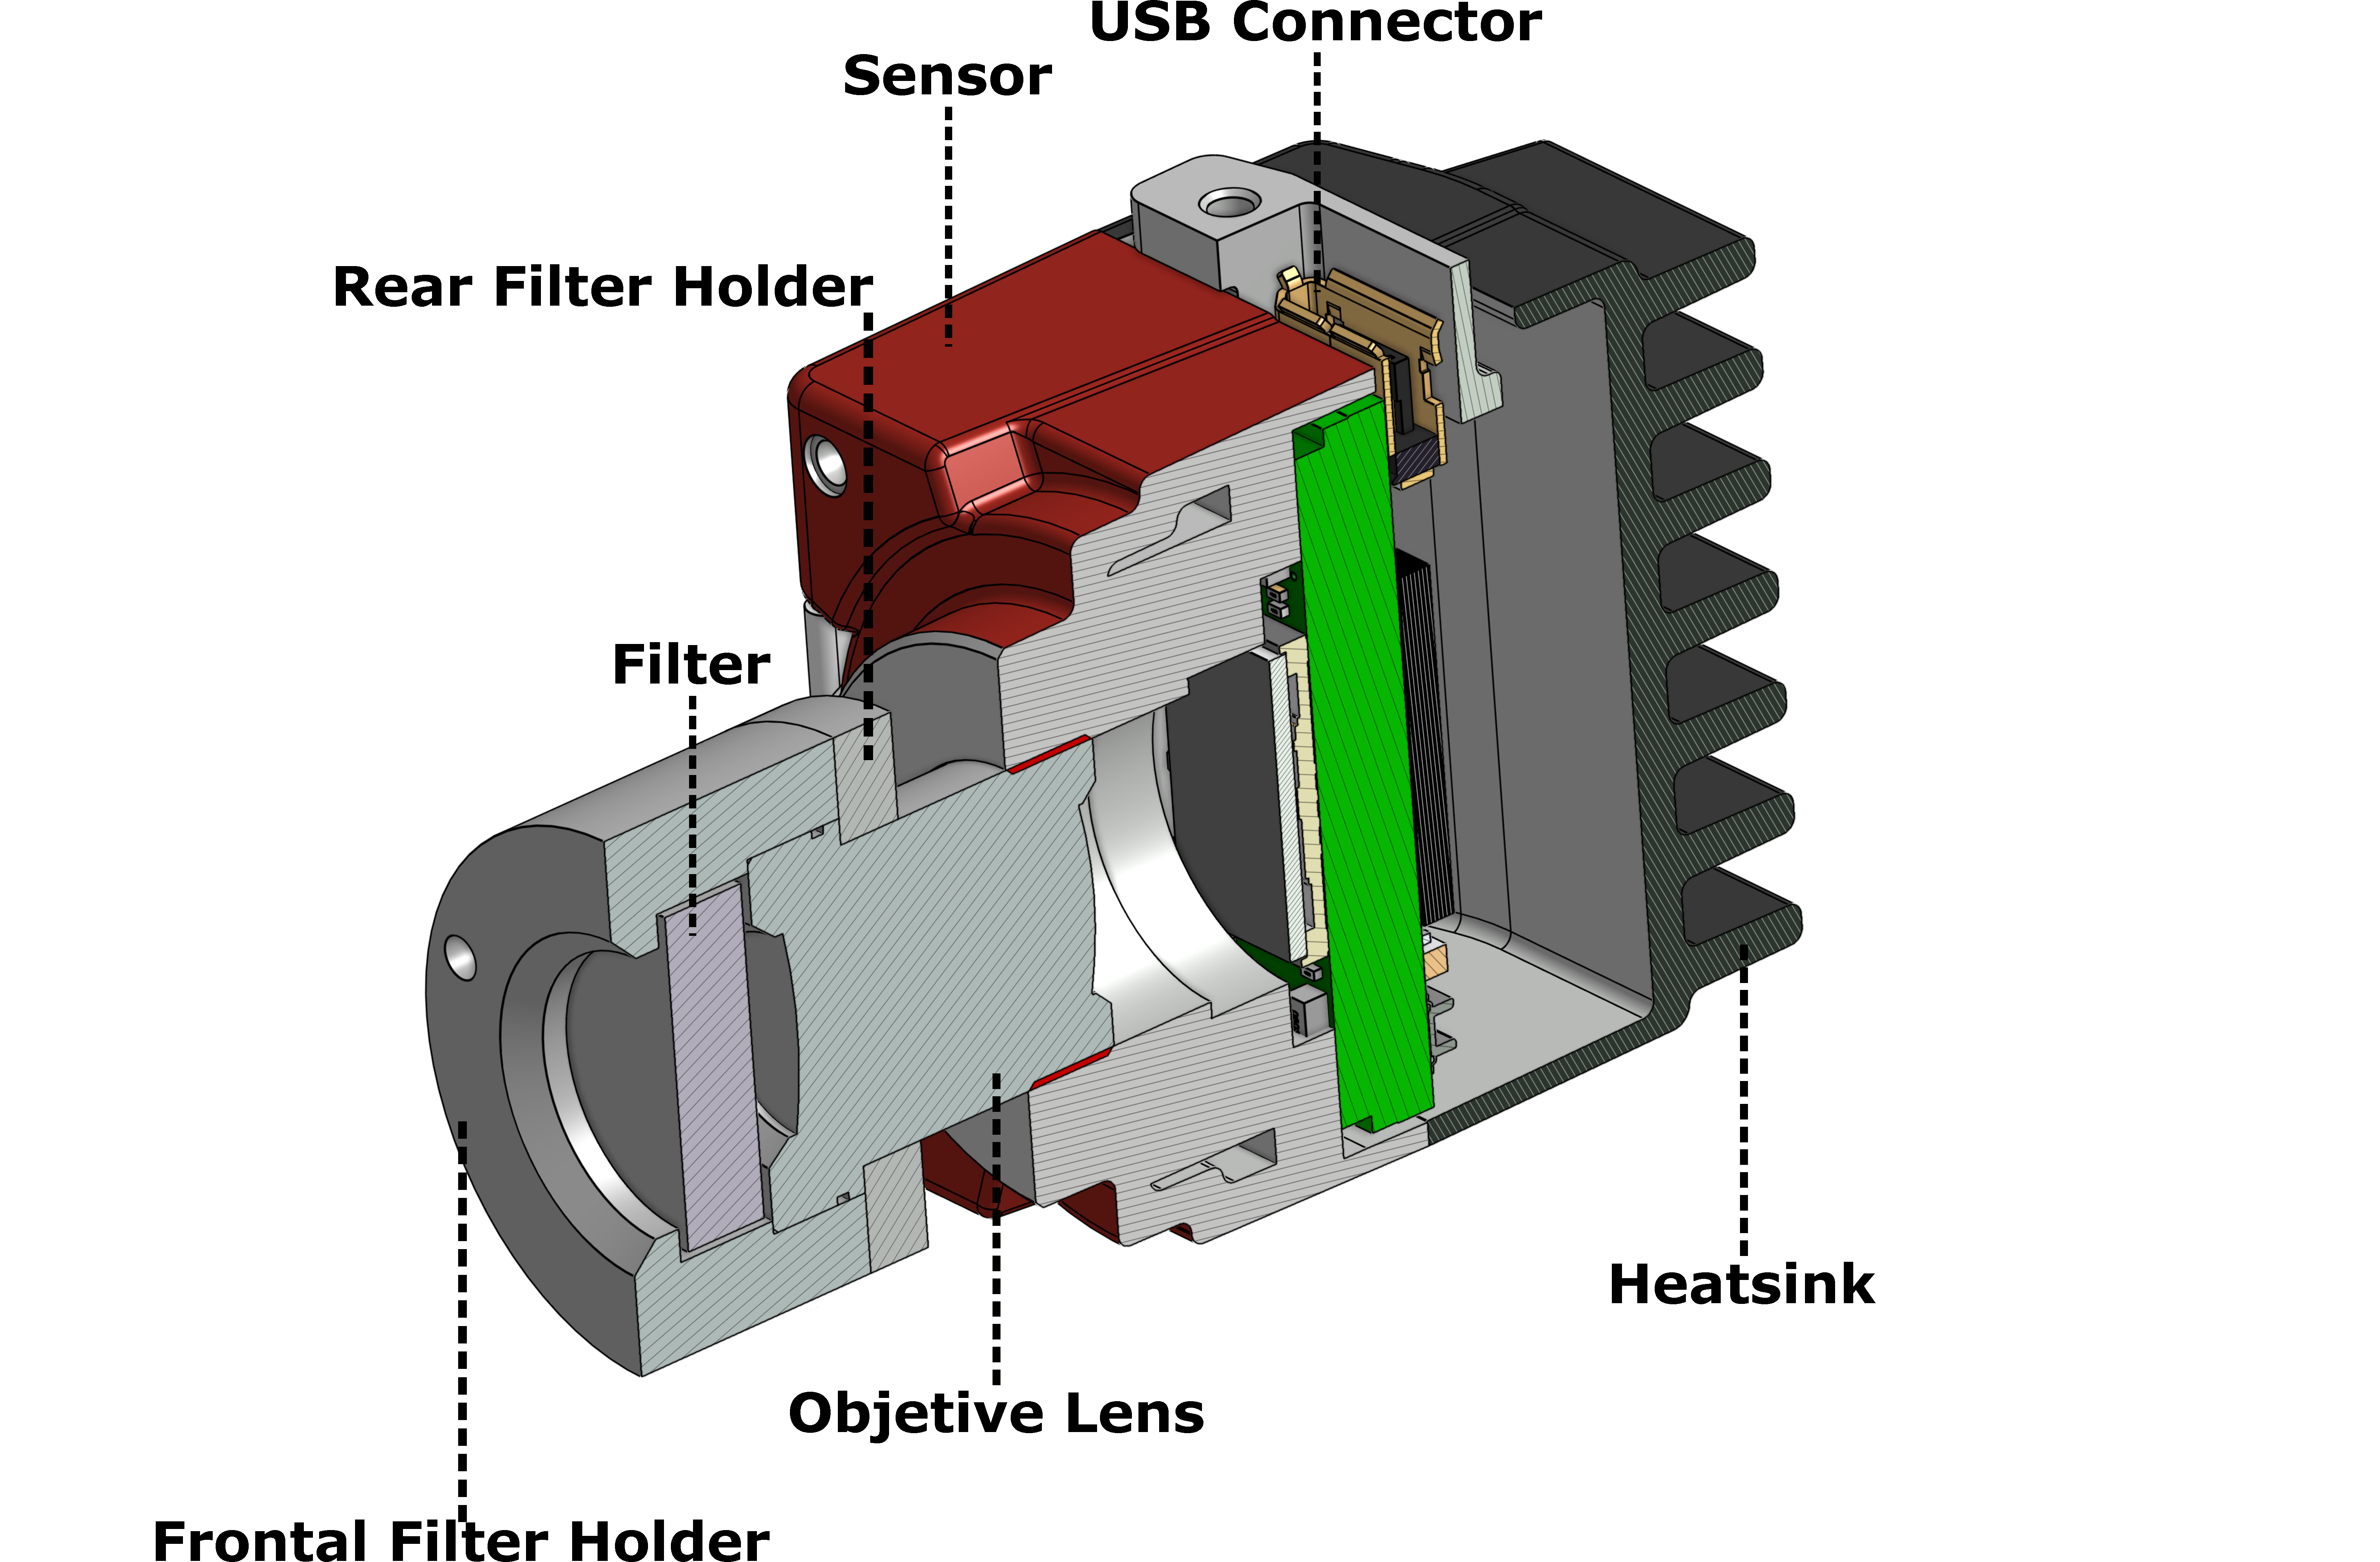
\includegraphics[width=\linewidth]{Figures/C4/NIR1.pdf}
        \caption{Sistema 6 (NIR): montaje del objetivo y filtro. El soporte evita desalineamientos y asegura la óptica en su eje.}
        \label{fig:lens_filter_mount_nir}
    \end{subfigure}
    \hfill
    \begin{subfigure}[b]{0.47\linewidth}
        \centering
        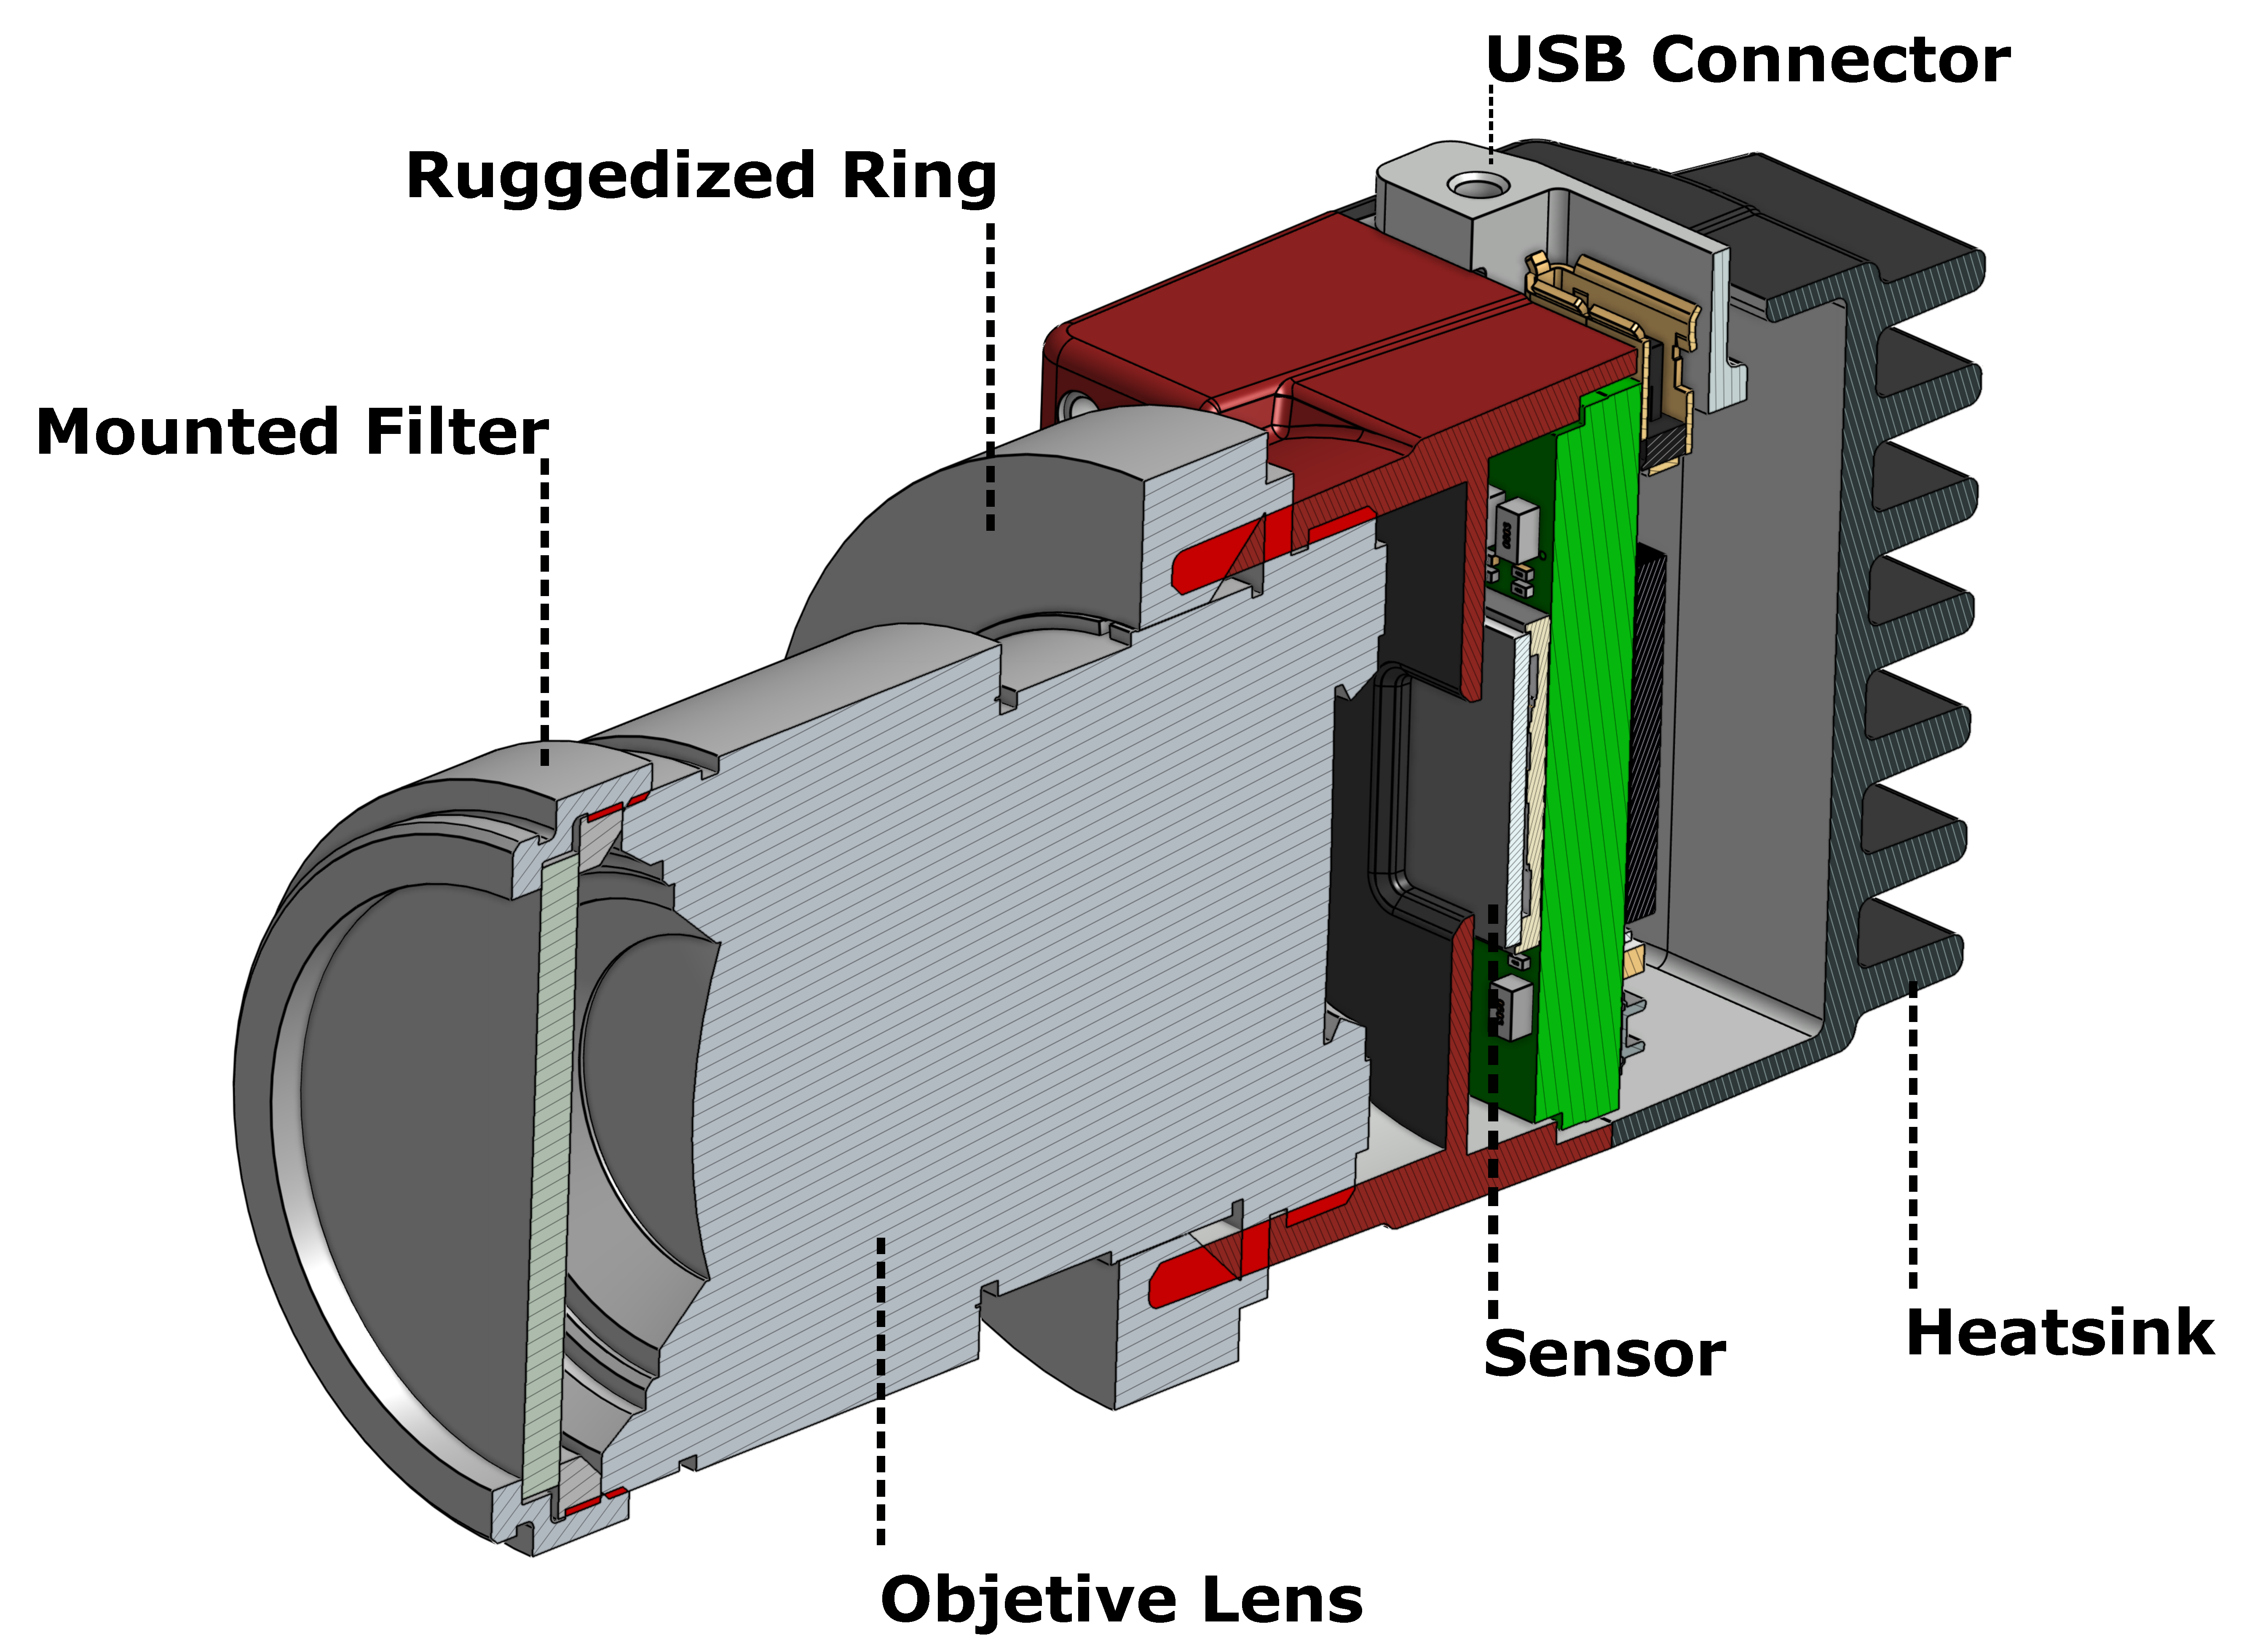
\includegraphics[width=\linewidth]{Figures/C4/VIS1.pdf}
        \caption{Sistema 7 (VIS): conector micro USB‑B para alimentación y datos.}
        \label{fig:micro_usb_vis}
    \end{subfigure}
    \caption{Componentes destacados de los sistemas ópticos seleccionados para el prototipo: NIR (izquierda) y VIS (derecha).}
    \label{fig:sistemas_opticos_componentes}
\end{figure}


  % \subsection{Integración con la plataforma UAV}
  %   % → Describir interfaz mecánica, centro de masas, cableado
  %   %   y sistema de amortiguación de vibraciones.

  % \subsection{Validaciones funcionales de taller}
  %   % → Pruebas de alineamiento, sellado de luz parásita y peso final.
  %   %   Tabla de verificación contra los requisitos de la Sección 1.1.
  \section{Sistema de adquisicion y control de datos}
  \label{sec:script_control_adquisicion}
  
  Con el propósito de automatizar el proceso de captura, procesamiento y almacenamiento de imágenes multiespectrales durante los vuelos o pruebas en banco, se desarrolló un script en lenguaje Python que permite la adquisición simultánea de imágenes en el espectro visible (VIS) y cercano al infrarrojo (NIR), integrando además datos de posicionamiento global (GPS) en tiempo real.
  
  \noindent Este script constituye una adaptación del código de ejemplo provisto por la biblioteca \texttt{vmbpy}, correspondiente al SDK de \textit{Allied Vision}, y fue modificado sustancialmente para incluir manejo multihilo, escritura condicional de video, superposición de información telemétrica, y control por teclado durante la ejecución.
  
  \subsection{Estructura general del script}
  
  El flujo lógico del código se presenta en la Figura~\ref{fig:diagrama_script}, donde se destacan tres etapas fundamentales: (i) la inicialización del entorno y detección de cámaras, (ii) la adquisición concurrente de tramas mediante hilos productores, y (iii) el procesamiento y visualización de las imágenes mediante un hilo consumidor.
  
  \begin{figure}[!h]
      \centering
      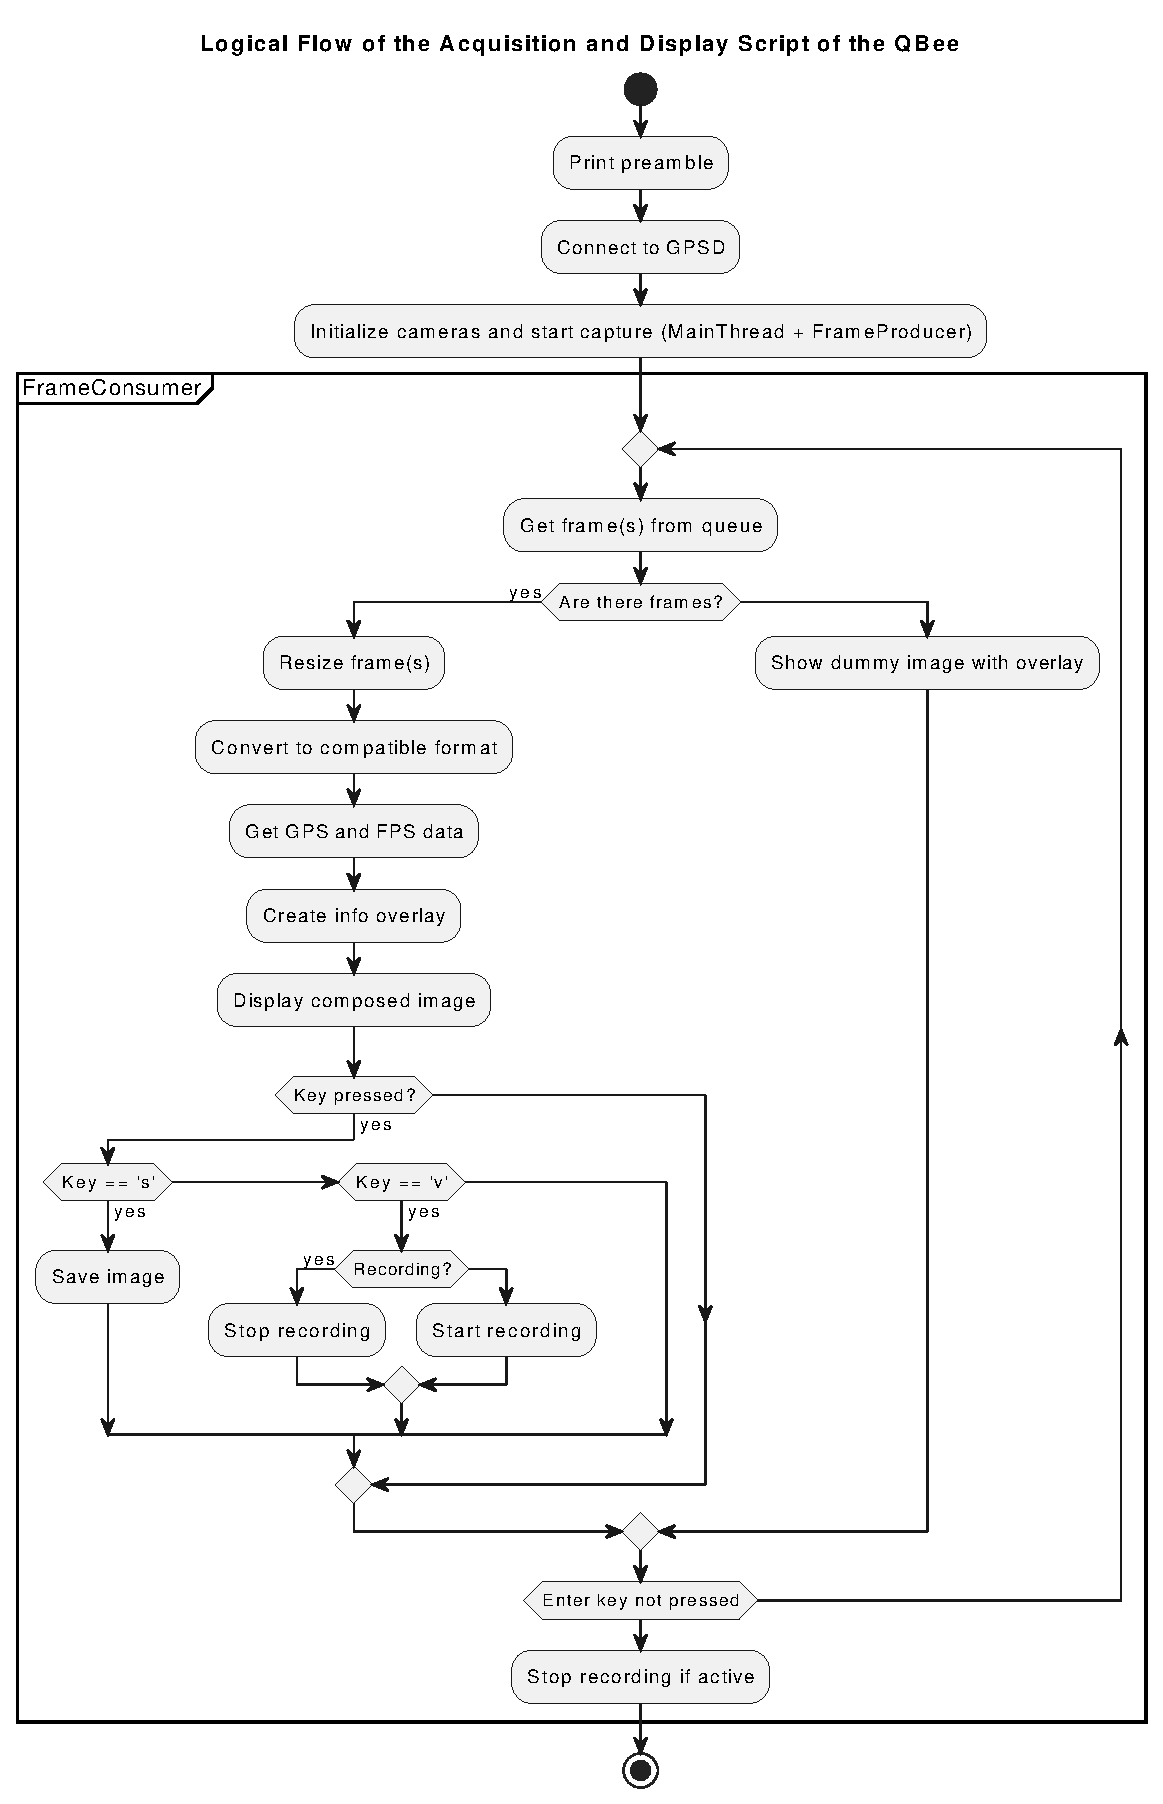
\includegraphics[trim = 0 0 0 1cm, clip, width=1\textwidth]{Figures/C4/OSU_main.pdf}
      \caption{Flujo lógico del script de adquisición y visualización de la QBee. Se integran múltiples cámaras, adquisición en paralelo y procesamiento en tiempo real.}
      \label{fig:diagrama_script}
  \end{figure}
  
  \subsection{Inicialización y adquisición}
  
  Durante la fase de inicialización, se establece una conexión con el servidor local de GPS (\texttt{gpsd}) utilizando la librería homónima. Paralelamente, se instancia la clase \texttt{MainThread}, responsable de detectar automáticamente todas las cámaras conectadas a través del sistema \texttt{VmbSystem}.\\
  
   Cada cámara detectada es asignada a un hilo independiente de la clase \texttt{FrameProducer}, la cual configura parámetros críticos como la resolución de adquisición, formato de pixel (\texttt{Mono8} o \texttt{Bgr8}), y el modo automático de exposición. Estos hilos se encargan de capturar tramas en tiempo real, estimar la tasa de cuadros por segundo (FPS) y encolar las imágenes en una estructura tipo FIFO (\texttt{queue.Queue}) para su posterior procesamiento.
  
  \subsection{Procesamiento, visualización y almacenamiento}
  
  La etapa central del sistema está contenida en la clase \texttt{FrameConsumer}, la cual opera como hilo consumidor. Esta clase realiza múltiples tareas en paralelo: (i) extrae tramas de la cola compartida, (ii) redimensiona las imágenes si la resolución de adquisición no coincide con la esperada (\SI[parse-numbers = false]{2592 \times 1944}{px}), (iii) convierte los formatos de imagen a RGB si es necesario, y (iv) concatena las imágenes capturadas por múltiples cámaras en un único mosaico horizontal.\\
  
  Sobre esta imagen compuesta se genera una barra de información (\textit{overlay}) que incluye los datos georreferenciados en tiempo real (latitud, longitud, altitud, velocidad, ángulo de rumbo y timestamp), además de la tasa de cuadros por segundo estimada para cada cámara. Esta superposición se construye como una matriz adicional que se apila verticalmente a la imagen original.\\
  
  El sistema también permite una interacción directa con el operador mediante teclas específicas:
  \begin{itemize}
      \item \textbf{\texttt{s}}: captura la imagen actual y la guarda en formato \texttt{JPEG}.
      \item \textbf{\texttt{v}}: inicia o detiene la grabación de video en formato \texttt{AVI}, con compresión \texttt{XVID}, a una frecuencia de 20 FPS.
      \item \textbf{\texttt{Enter}}: finaliza la ejecución del script y cierra todas las ventanas.
  \end{itemize}
  
  \subsection{Ejecución automática como servicio de sistema}
  
  Con el fin de garantizar un funcionamiento autónomo y minimizar la intervención del usuario, se diseñó un servicio de sistema en Linux (utilizando \texttt{systemd}) que permite la ejecución automática del script tan pronto como el dispositivo inicia. Este servicio fue instalado y habilitado en el sistema operativo de una Raspberry Pi 4 modelo B equipada con 8 GB de memoria RAM.
  
  Gracias a esta configuración, el sistema conocido como \texttt{QBee} se activa automáticamente al conectar la batería externa a la Raspberry Pi, sin requerir intervención adicional ni acceso al entorno gráfico. Inmediatamente después del arranque, el script inicia la captura de imágenes y comienza a almacenarlas en la memoria interna, lo que resulta particularmente útil para operaciones en campo, donde no es viable iniciar el sistema manualmente.
  
  \subsection{Robustez y tolerancia a fallos}
  
  Durante la ejecución, el sistema cuenta con mecanismos de tolerancia a errores. Por ejemplo, si el buffer de imágenes se encuentra lleno, los hilos productores omiten la encolación de nuevas tramas para evitar bloqueos. Asimismo, si no se detecta ninguna cámara activa, se genera una imagen dummy con un mensaje de advertencia.\\
  
  Las tramas obtenidas se almacenan temporalmente en memoria, lo que permite minimizar la latencia entre adquisición y visualización. La sincronización entre hilos se realiza mediante eventos y bloqueos controlados, garantizando la integridad de los datos entre productores y consumidores.
  
  \subsection{Dependencias y entorno de ejecución}
  
  El script fue ejecutado sobre el sistema operativo Raspberry Pi OS (basado en Debian) en una Raspberry Pi 4 modelo B. Se utilizó Python 3.8 y las siguientes dependencias: \texttt{vmbpy}, \texttt{opencv-python}, \texttt{gpsd-py3}, \texttt{numpy}, \texttt{threading}, \texttt{queue} y \texttt{keyboard}. La visualización se realizó mediante la salida HDMI de la Raspberry, y se requirió establecer la variable de entorno \texttt{DISPLAY=":0"} para habilitar la salida gráfica de OpenCV.

  \subsection{Control remoto del dispositivo \texttt{QBee}}

  Además de su capacidad de operación autónoma en campo, el sistema \texttt{QBee} fue diseñado con funcionalidad de control remoto, permitiendo su supervisión y operación desde dispositivos externos como computadores personales, tabletas o teléfonos móviles. Esta característica extiende significativamente la versatilidad del sistema, facilitando tanto pruebas en laboratorio como operaciones a distancia en entornos de difícil acceso.\\
  
  Existen dos métodos principales para acceder de forma remota a la interfaz gráfica del sistema:
  
  \paragraph{1. Conexión local mediante VNC}
  
  El primer método consiste en conectarse directamente a la Raspberry Pi 4 que ejecuta el sistema \texttt{QBee} mediante el protocolo VNC (\textit{Virtual Network Computing}). Para ello, es necesario que la Raspberry esté conectada a una red Wi-Fi previamente configurada para su conexión automática. Asimismo, el dispositivo de control (computador o móvil) debe encontrarse dentro de la misma red local.\\
  
  Una vez cumplida esta condición, el usuario puede acceder a la interfaz gráfica de la Raspberry Pi introduciendo su dirección IP o una dirección local estática configurada mediante el sistema operativo Raspberry Pi OS. Para completar el acceso, se requiere conocer las credenciales de autenticación (nombre de usuario y contraseña) establecidas previamente en el sistema.
  
  \paragraph{2. Acceso global mediante Raspberry Pi Connect}
  
  El segundo método se basa en el uso de \textit{Raspberry Pi Connect}, un servicio gratuito proporcionado por la fundación Raspberry Pi. Este permite acceder a la interfaz gráfica del sistema desde cualquier lugar con conexión a Internet, sin necesidad de estar dentro de la misma red local.\\
  
  Para habilitar esta funcionalidad, la Raspberry Pi debe estar vinculada a una cuenta en el servicio \textit{Raspberry Pi Connect} y tener acceso a Internet mediante una red Wi-Fi registrada previamente. Una vez registrado el dispositivo, el usuario puede iniciar sesión en el portal de Raspberry Pi y conectarse directamente a su interfaz gráfica a través del navegador.  \\
  
  
  En ambos métodos, el usuario obtiene acceso completo al entorno de escritorio de la Raspberry Pi. Como se ha descrito en las secciones anteriores, el script de adquisición de \texttt{QBee} se ejecuta automáticamente al iniciar el sistema, lo que da lugar a la apertura de una ventana de visualización en tiempo real de las imágenes capturadas.\\
  
  Desde esta interfaz remota, el usuario puede interactuar directamente con el sistema utilizando un teclado virtual o físico para ejecutar acciones de control. Entre las funcionalidades disponibles se encuentran:
  \begin{itemize}
      \item Presionar la tecla \texttt{s} para capturar y guardar una imagen.
      \item Presionar la tecla \texttt{v} para iniciar o detener la grabación de video.
      \item Presionar la tecla \texttt{Enter} para finalizar la ejecución del script.
  \end{itemize}
  
  Esta capacidad de control remoto permite verificar el correcto funcionamiento del sistema en tiempo real, supervisar condiciones de operación, y capturar eventos relevantes sin necesidad de intervención física directa sobre el dispositivo.\\
  
  
  Adicionalmente, el sistema \texttt{QBee} fue configurado para permitir actualizaciones remotas del código fuente del script mediante el sistema de control de versiones \texttt{Git}. El script está vinculado a un repositorio privado alojado en la plataforma \texttt{GitHub}, lo que permite a los usuarios autenticados realizar \textit{pull} de actualizaciones desde cualquier ubicación con acceso remoto al dispositivo. Esta funcionalidad permite una mejora continua del sistema, facilitando la depuración, implementación de nuevas funcionalidades y adaptaciones específicas sin necesidad de acceso físico al hardware.
  

  \section{Construcción e integración del prototipo}
  \subsection{Modelo CAD y ensamblaje mecánico}
    % → FIGURA grande: render CAD explosionado del KBee con leyenda de partes.
    %   Tabla: materiales y masa de cada componente.

    El case del QBee está impreso en PET‑G (tereftalato de polietileno modificado con glicol), un polímero cuya densidad típica ronda 1,317 g/cm³, que combina buena resistencia al impacto (Charpy $\approx$ 4,03 kJ/m²) y alargamiento al rompimiento hasta 15\% en formulaciones estándar. Su módulo de tracción (~4015 MPa) y de flexión (~2987 MPa) aseguran rigidez, mientras que su temperatura de transición vítrea ($\approx$ 76 °C) y rango de fusión (220–260 °C) lo hacen estable en el calor generado por electrónica cercana. Además, presenta excelente durabilidad química y mínima tendencia al \emph{warping}, ideal para piezas de geometría compleja. El peso total del disposito es de 1.810 gramos, cumpliendo así con el requisito de peso impuesto.\\

    \noindent La dimensión externa del case se diseñó para encajar en el bay interno del UAV C3, sin requerir hermeticidad, ya que este estária protegido de las condiciones exteriores. El cierre se logra con tornillos M3 que unen la tapa inferior y el divisor de compartimentos a la carcasa principal. En el interior, cada sistema óptico (6/NIR y 7/VIS) se ancla directamente al sensor mediante cuatro tornillos M3 en sus laterales, asegurando alineación con el eje de vuelo. El sistema 6 (NIR) monta el Alvium 1800 U‑501m (AR0522) + objetivo 8 mm f/2.5 + filtro 850 nm en montura S, todo encapsulado en una montura de resina 3D. El sistema 7 (VIS) agrupa el Alvium 1800 U‑500c (AR0521) + objetivo 8.5 mm f/1.3 ruggedized + filtro VIS UV/IR Cut en rosca M25.5, manteniendo rigidez frente a vibraciones.\\
    
    \noindent La unidad de cómputo y almacenamiento es una Raspberry Pi 4, colocada en un bloque intermedio y alimentada por una powerbank de 20.000 mAh. Este sistema tiene acoplado un hat de GPS, que suministra al sistema de metadatos de fecha, hora UTC, latitud, longitud, altitud y ángulo de elevación, esenciales para la georreferenciación y ortorrestitución de imágenes. Finalmente, el módulo in situ de sensado de contaminantes comparte alimentación de 5 V de la misma batería y ocupa el compartimento trasero de la carcasa, completando la funcionalidad del QBee.\\
    
    

    \begin{figure}[h]
        \centering
        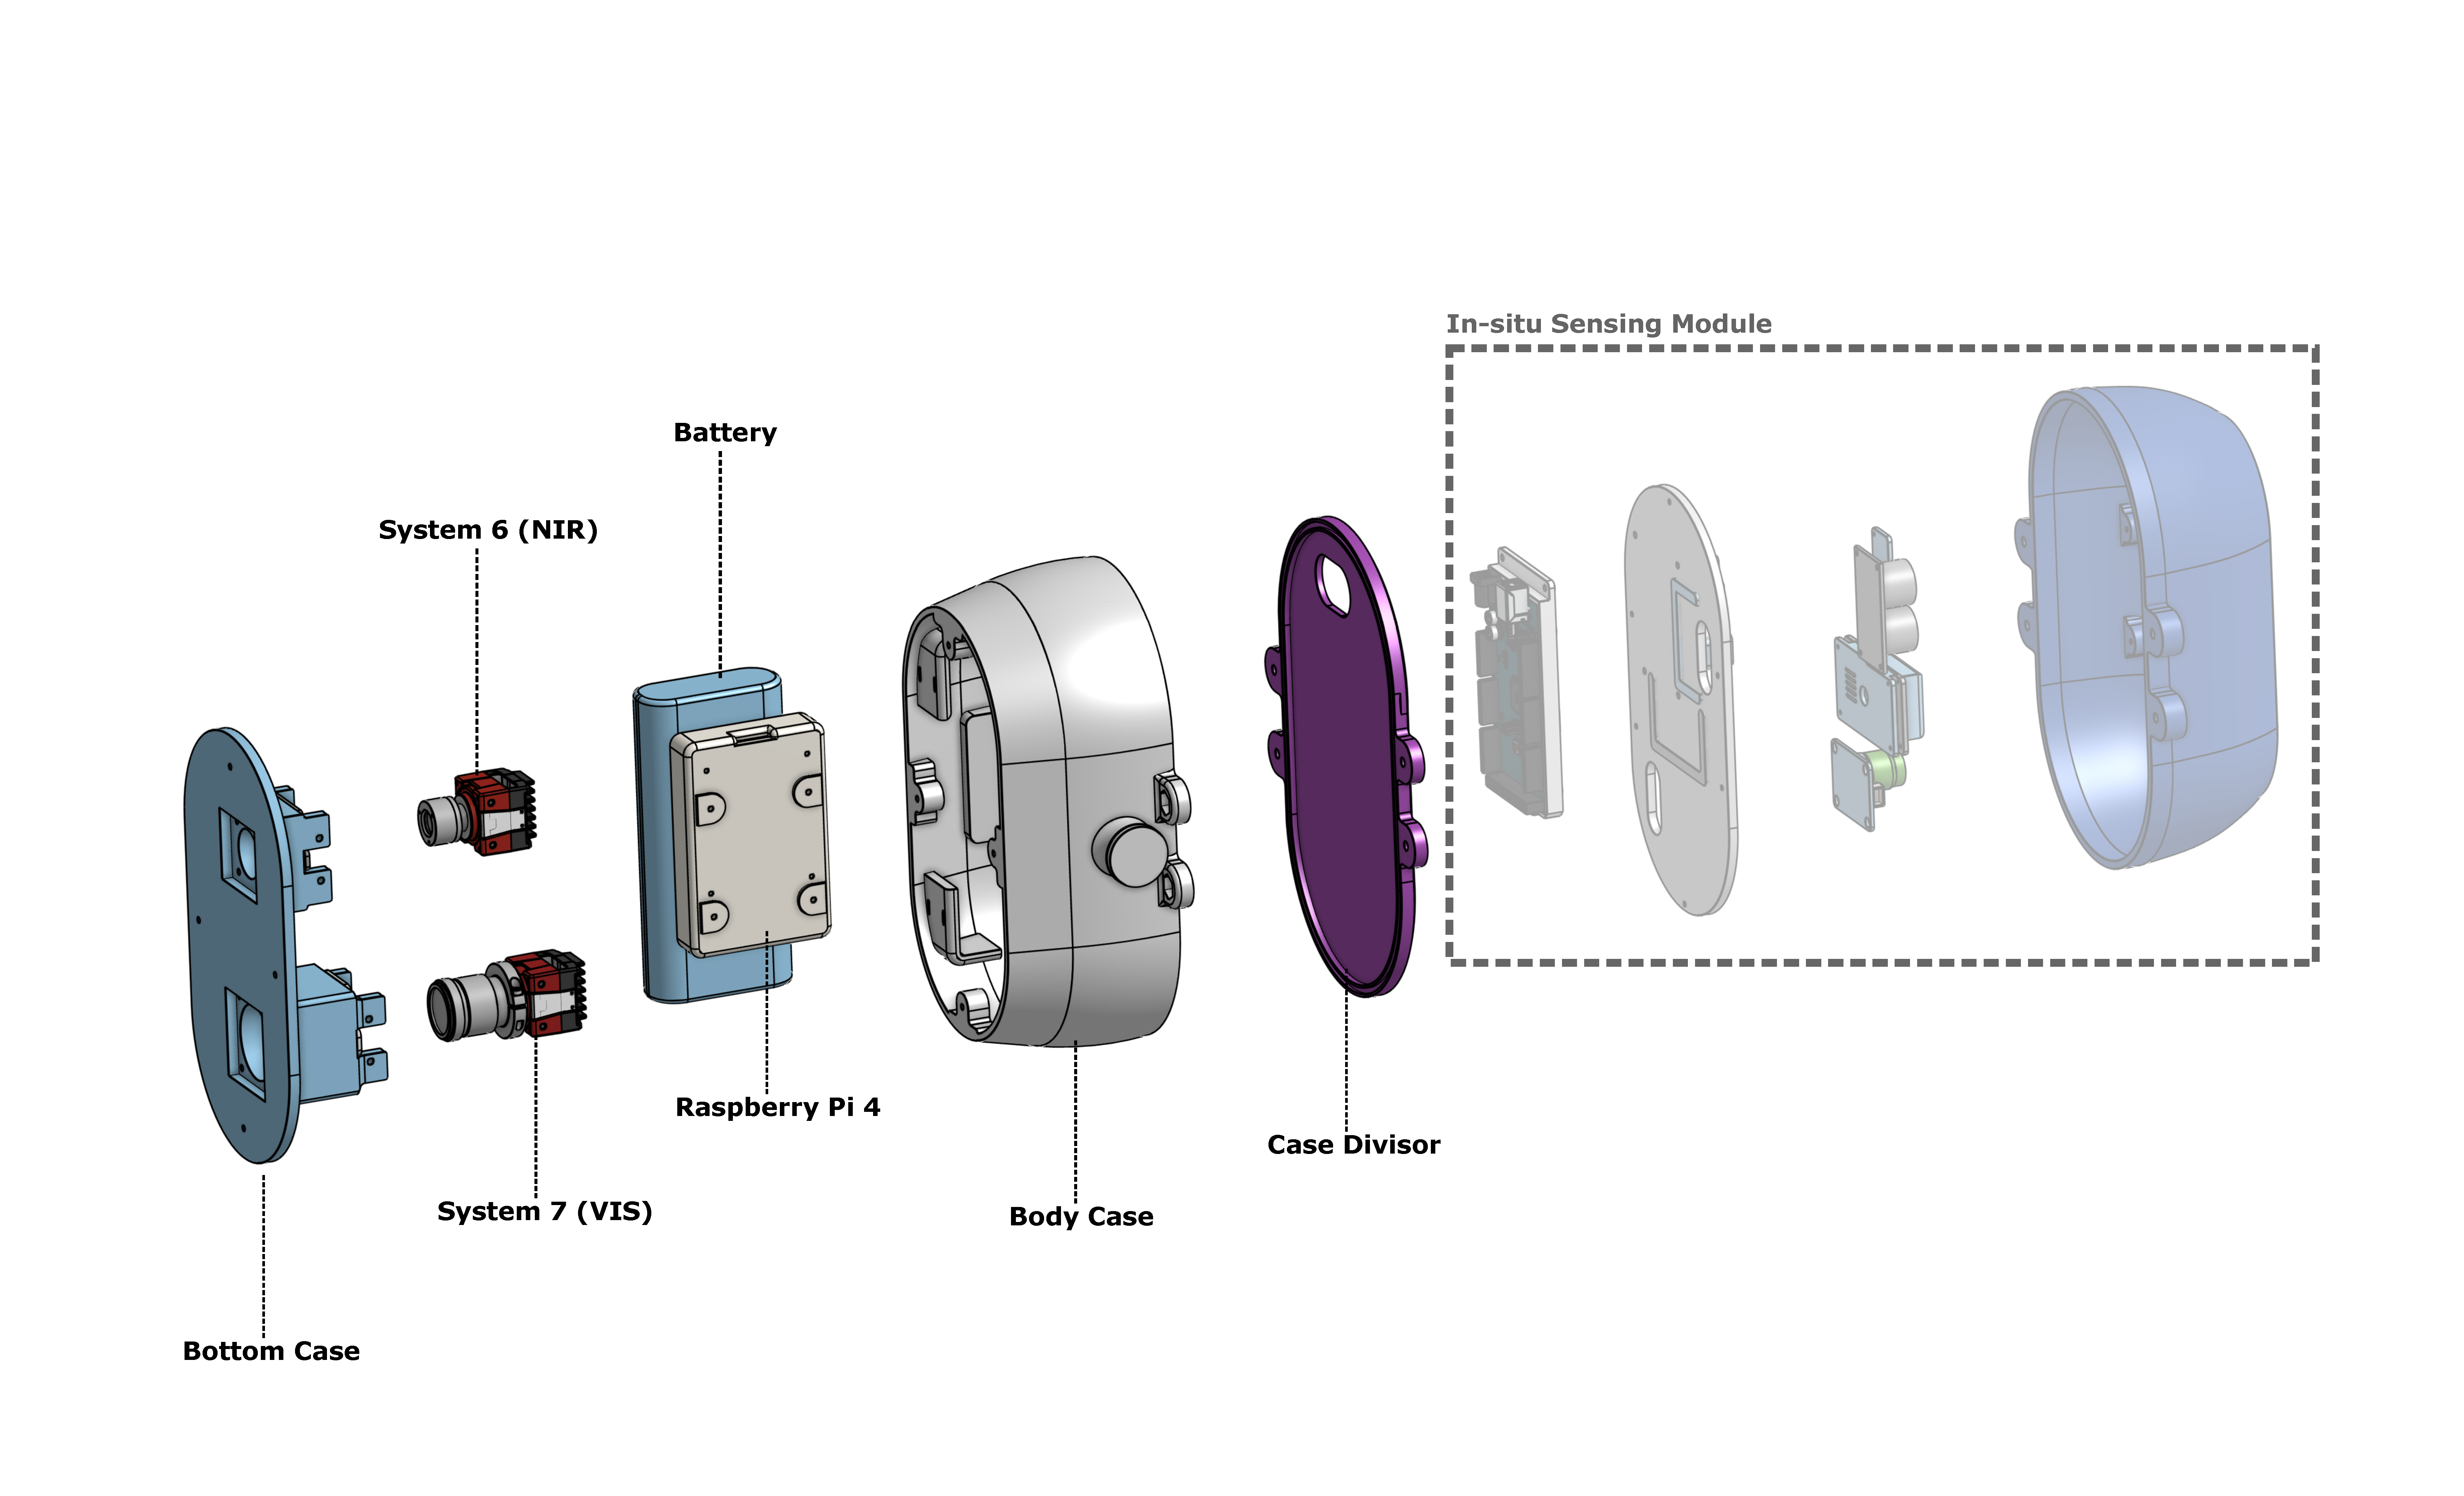
\includegraphics[width=1\linewidth]{Figures/C4/QBee.pdf}
        \caption{Vista explosionada del ensamble completo del QBee, mostrando la carcasa impresa en PET‑G y la disposición de los sistemas 6 (NIR, 8 mm f/2.5) y 7 (VIS, 8.5 mm f/1.8). Este diseño y construcción fue concebido con el apoyo del equipo de manufactura del pryecto C3.}
        \label{fig:exploded_assembly}
    \end{figure}

 

\section{Pruebas de operación}
  
  
  \subsection{Escenarios de prueba}
    Los escenarios de prueba definidos para validar el correcto funcionamiento del sistema \textit{QBee} se clasifican en dos grupos principales: (i) pruebas terrestres en condiciones controladas, y (ii) pruebas en vuelo.

    \subsubsection{Pruebas terrestres}
    
        Antes de cualquier despliegue aéreo, es indispensable realizar pruebas en tierra que permitan validar el sistema en condiciones controladas, sin desplazamiento y sin exposición a ambientes extremos. En este contexto, se define como ambiente extremo cualquier entorno cuya temperatura supere los valores comunes encontrados en las principales ciudades colombianas (\SI{\leq 40}{\celsius}), o que implique lluvia, alta humedad o condiciones de iluminación nocturna.
        
        \noindent Dado que el sistema \textit{QBee} no cuenta con una fuente de iluminación activa, las pruebas se realizan exclusivamente durante el día, aprovechando la luz solar como fuente principal para la adquisición de imágenes multiespectrales.
        
        \noindent El objetivo de estas pruebas es verificar el comportamiento general del sistema en condiciones operativas normales. En particular, se evalúa:
        
        \begin{itemize}
        \item La correcta inicialización automática del script de adquisición al encender el dispositivo.
        \item La funcionalidad de captura de imágenes al presionar la tecla \texttt{s}.
        \item La grabación de video y su detención mediante la tecla \texttt{v}.
        \item La estabilidad del dispositivo al operar durante largos periodos de tiempo.
        \end{itemize}
        
        \noindent Las pruebas se realizaron utilizando dos formas de alimentación:
        \begin{itemize}
        \item \textbf{Fuente directa:} mediante un adaptador USB-C conectado a una toma de corriente convencional.
        \item \textbf{Fuente interna:} a partir de la bater'ia recargable integrada en la carcasa del \textit{QBee}.
        \end{itemize}
        
        \noindent Una de las pruebas más relevantes consisti'o en la captura de una imagen utilizando la tecla \texttt{s}, ya fuera desde un teclado conectado directamente a la Raspberry Pi 4 o mediante acceso remoto. En la Figura~\ref{fig:captura_prueba_remota} se presenta un ejemplo de imagen capturada en estas condiciones, utilizando un tel'efono inteligente para el control remoto del sistema. La prueba confirma el correcto funcionamiento de ambos canales (VIS y NIR), evidenciando que la captura simult'anea se realiza de manera sincronizada, y que el sistema responde adecuadamente a la orden de captura en tiempo real.
        
        \begin{figure}[h]
        \centering
        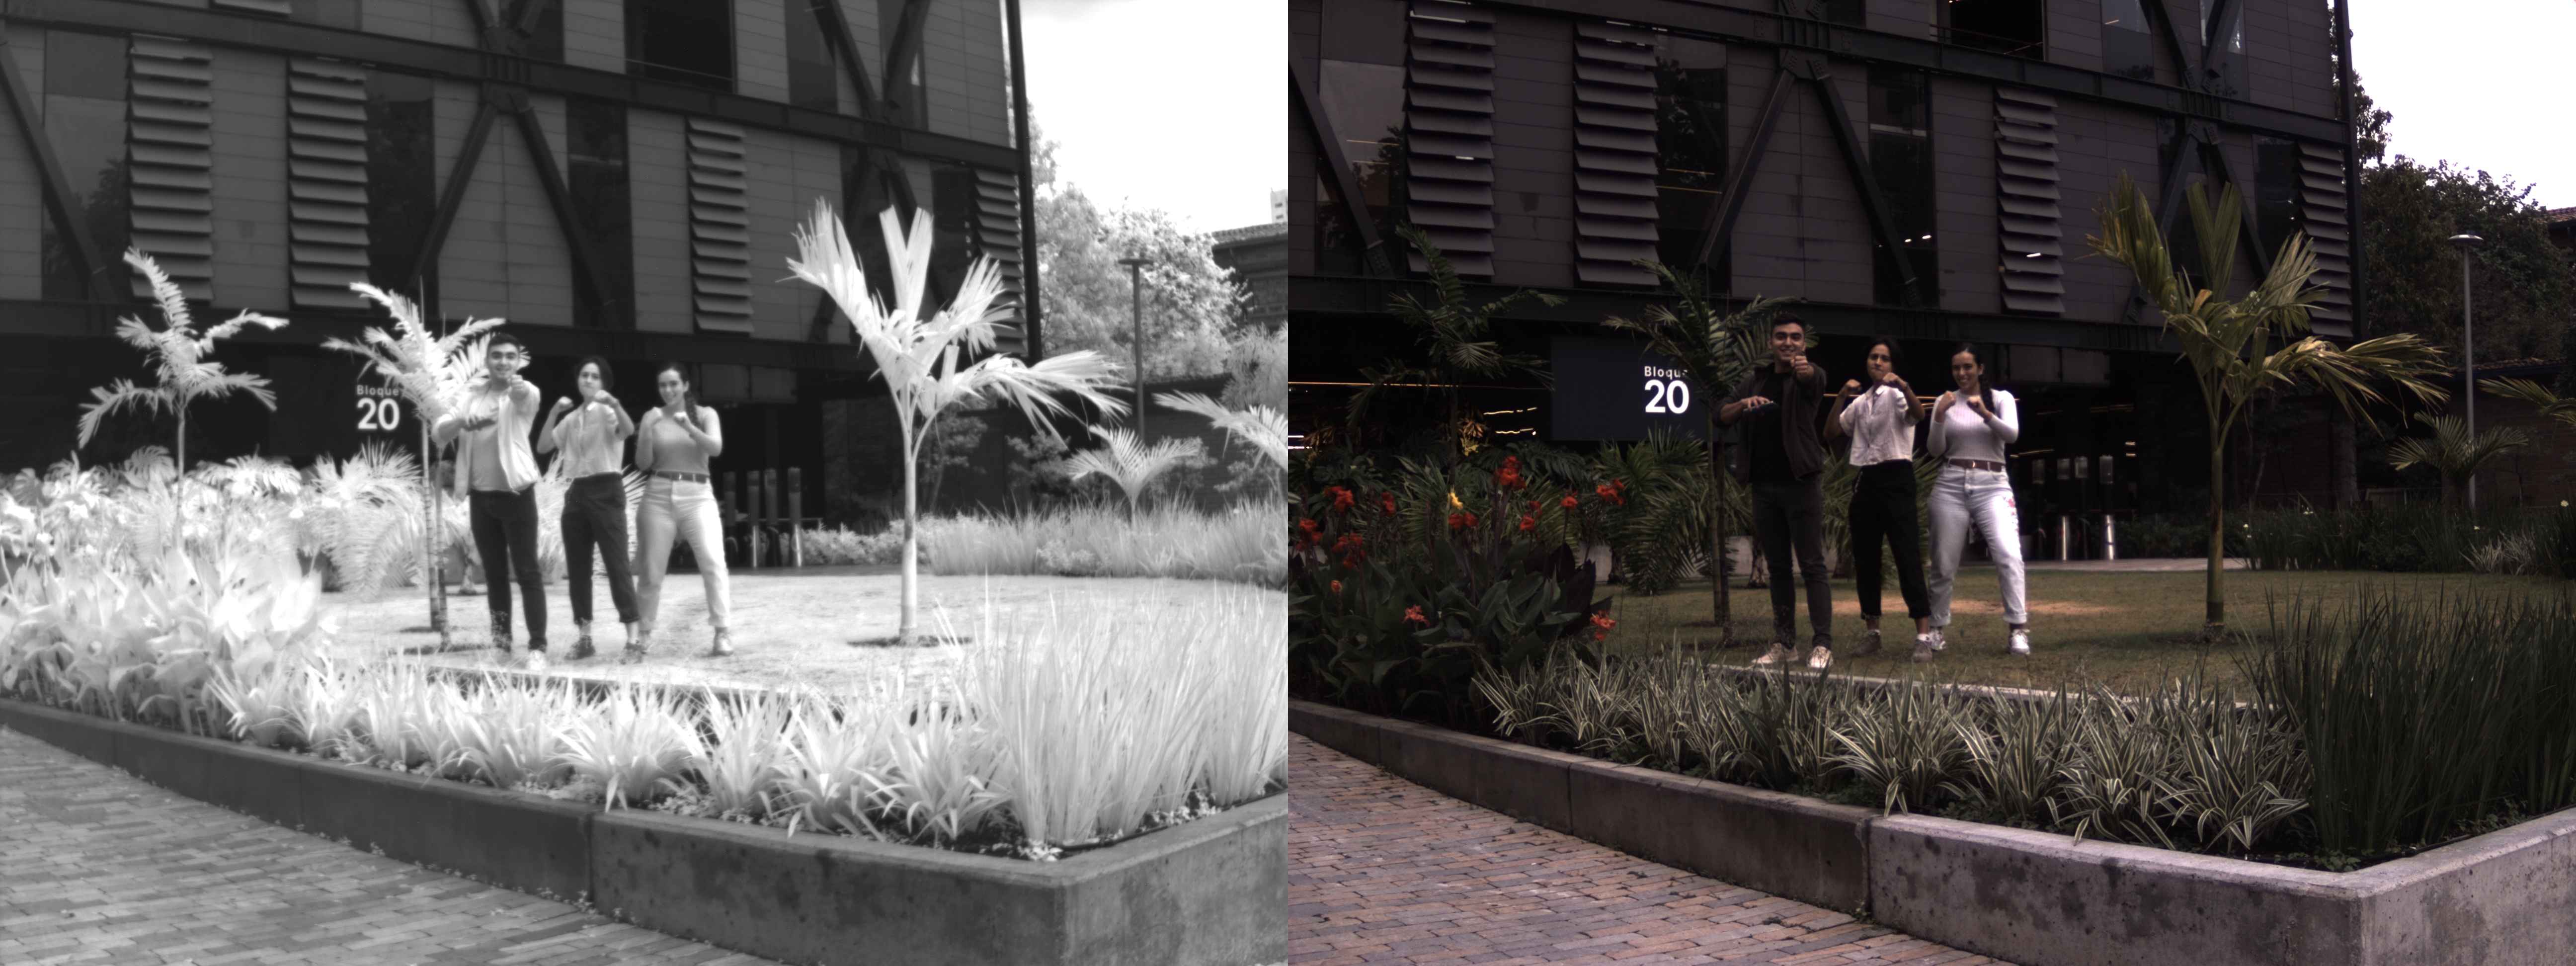
\includegraphics[width=1\textwidth]{Figures/C4/captured_image_20240201_174102.jpg}
        \caption{Captura de imagen realizada durante prueba terrestre mediante control remoto desde un tel'efono inteligente. La imagen muestra la composici'on de ambos canales VIS y NIR, confirmando la funcionalidad del sistema \textit{QBee} en condiciones operativas reales.}
        \label{fig:captura_prueba_remota}
        \end{figure}
        
        \noindent En complemento, en la Figura~\ref{fig:gps_overlay_visual} se presenta un ejemplo de visualización del sistema de coordenadas geográficas en tiempo real. En la parte superior de la imagen se observa la superposición del texto con la latitud, longitud, altitud, velocidad y rumbo extraídos del módulo GPS integrado en la \textit{QBee}. Esta funcionalidad es crítica para asegurar la trazabilidad espacial de las imágenes adquiridas y para su posterior georreferenciación.

        \begin{figure}[h]
            \centering
            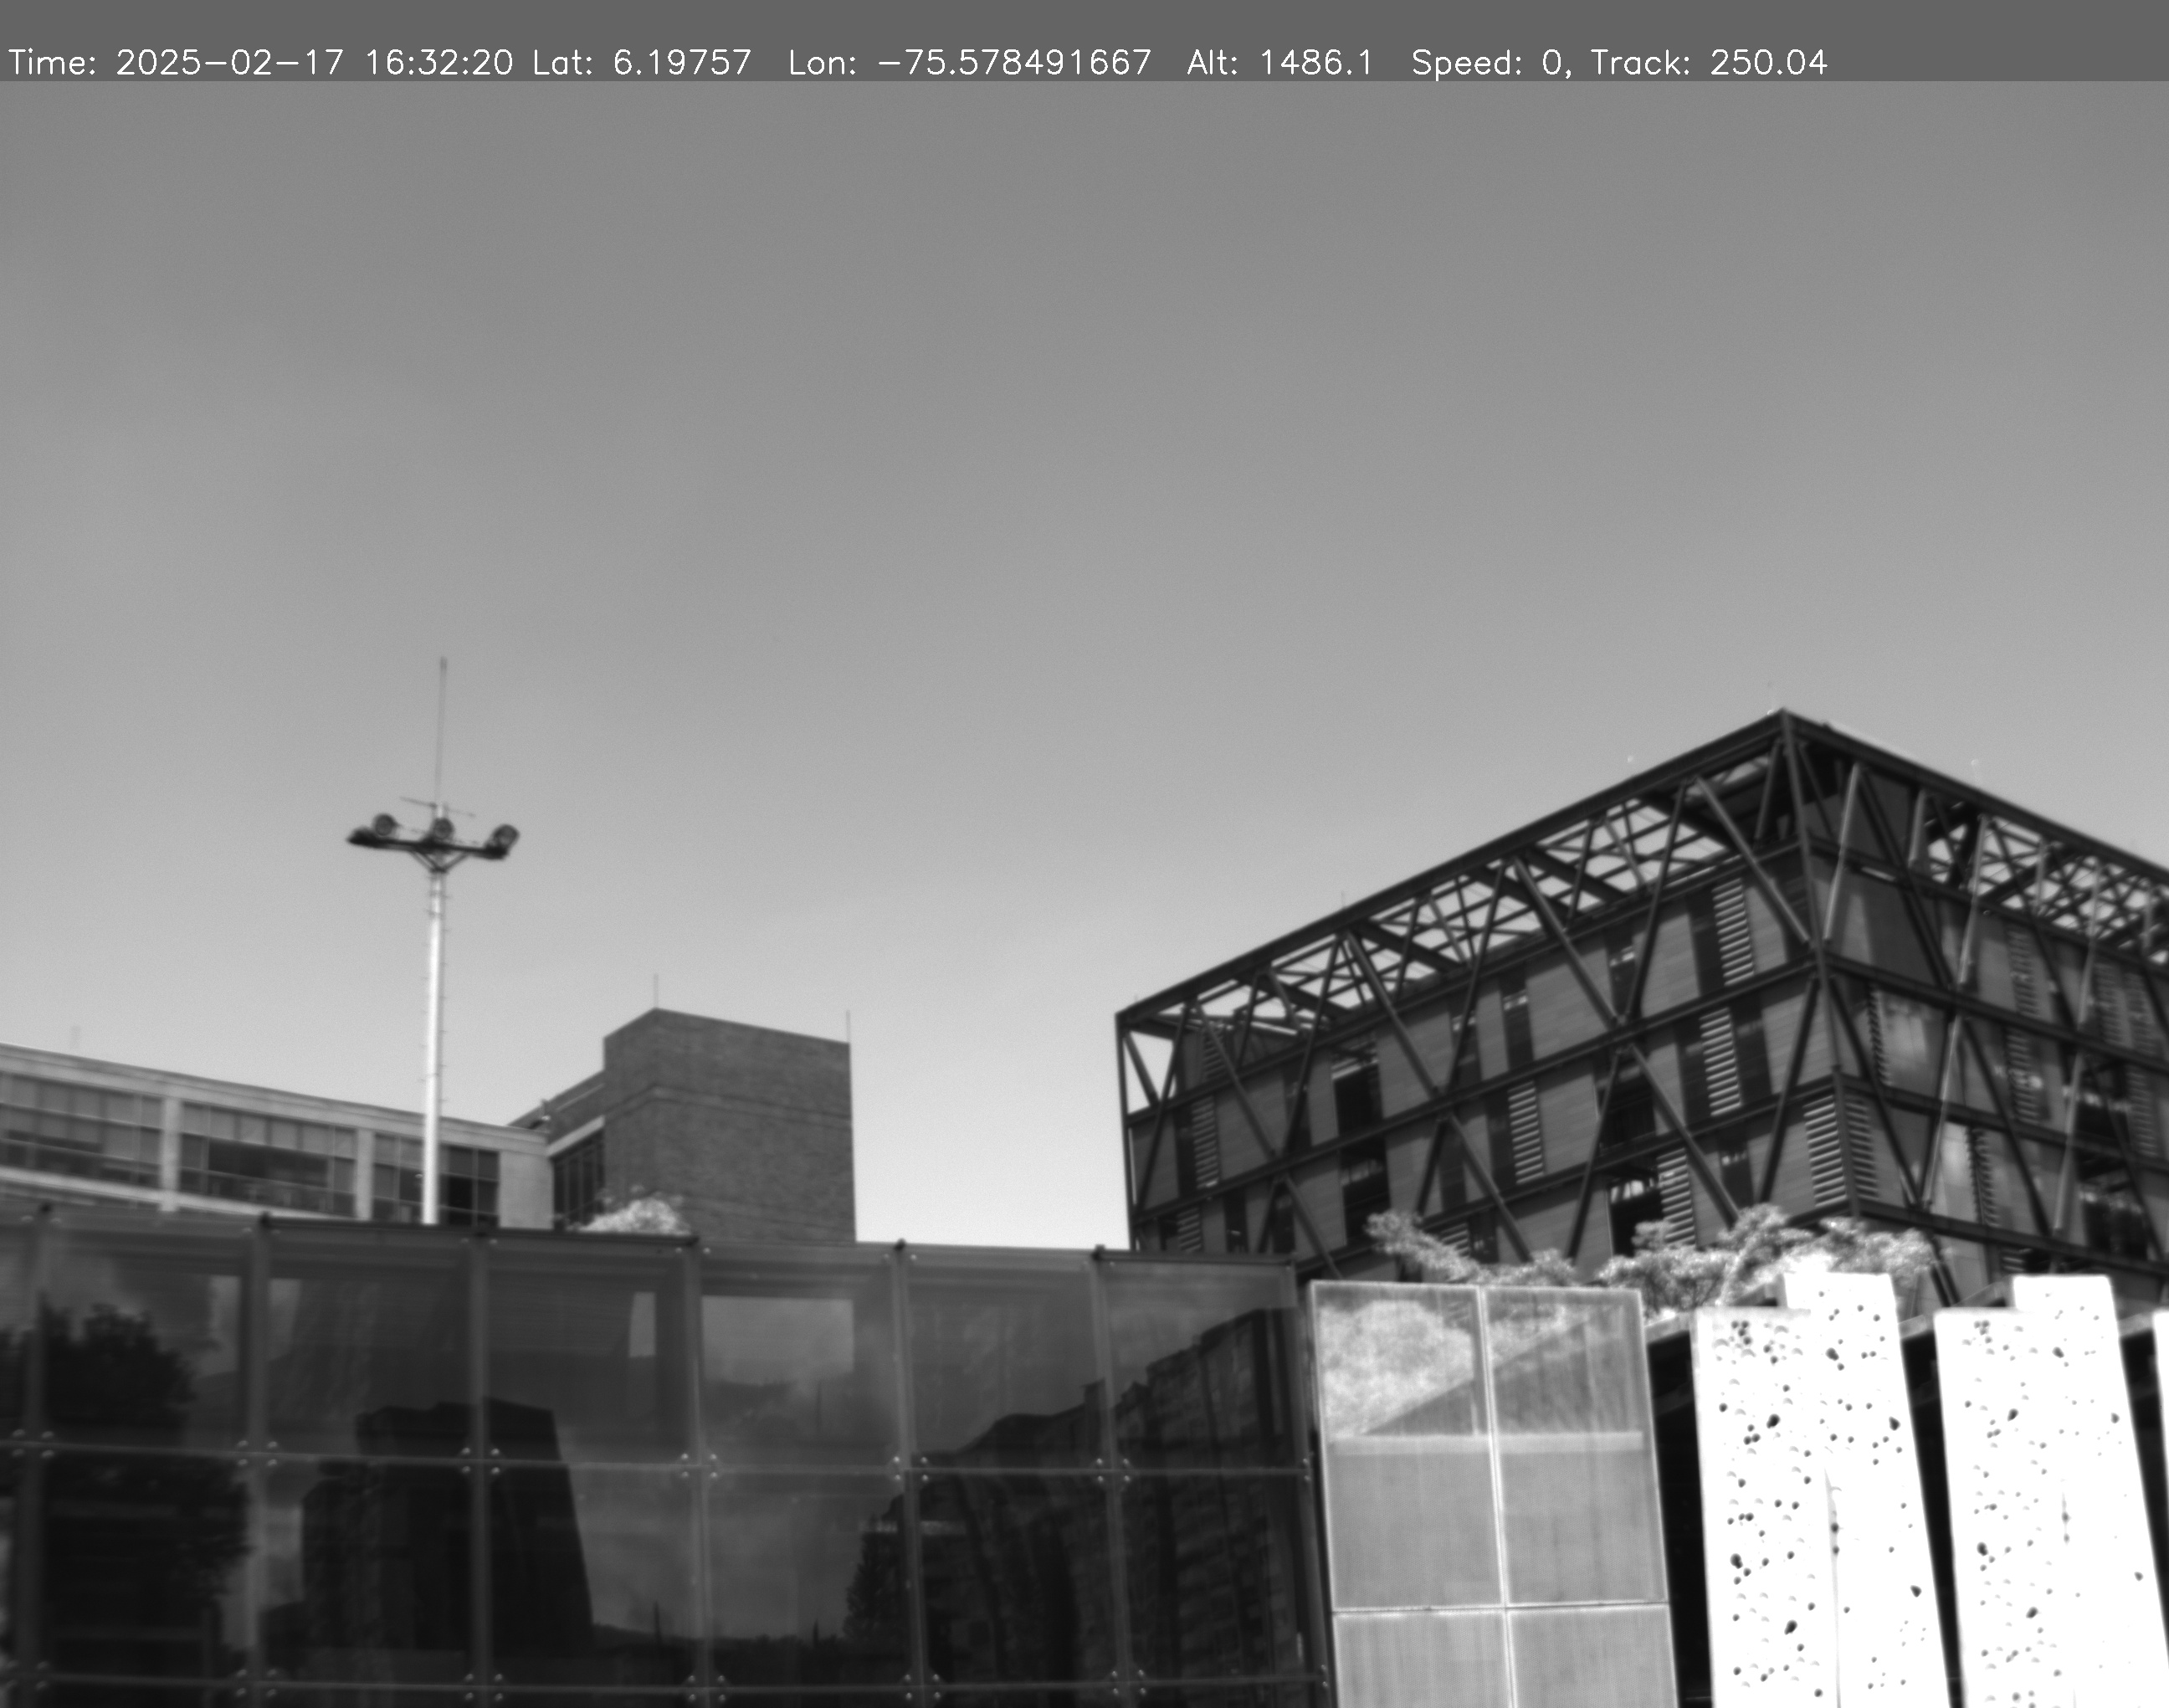
\includegraphics[width=0.9\textwidth]{Figures/C4/captured_image_20250217_113221.jpg}
            \caption{Visualización del sistema de coordenadas geográficas (GPS) en tiempo real sobre la imagen capturada. Se muestran latitud, longitud, altitud, velocidad y rumbo, extraídos automáticamente del módulo GPS durante las pruebas.}
            \label{fig:gps_overlay_visual}
        \end{figure}



    \subsubsection{Pruebas en superficie en condiciones extremas}

    Durante la VII Campa~na A'erea y XI Expedici'on Cient'ifica a la Ant'artida organizada por la Fuerza A'erea Colombiana, el sistema \textit{QBee} fue sometido a una prueba de funcionamiento en condiciones clim'aticas extremas. En este escenario, se enfrent'o a temperaturas diurnas promedio cercanas a los \SI{0}{\celsius}, significativamente inferiores a las condiciones habituales en las cuales opera el sistema.
    
    \noindent El objetivo principal de esta prueba fue evaluar la capacidad del dispositivo para operar de manera confiable en ambientes fr'ios. Se identific'o que, bajo estas condiciones, el sistema present'o fallas intermitentes en su funcionamiento: en algunas ocasiones la \textit{QBee} no inici'o correctamente, o no fue capaz de realizar la grabaci'on de video como lo hace regularmente. Estas fallas pueden estar asociadas a una inicializaci'on deficiente del sistema de procesamiento (Raspberry Pi 4), o a alteraciones en el comportamiento de los sensores VIS y NIR debido a la baja temperatura.
    
    \noindent No obstante, tambi'en se registraron casos exitosos de captura de video, lo cual demuestra que el sistema \textit{QBee} puede llegar a operar de forma funcional en condiciones de fr'io extremo. Estos resultados parciales abren la posibilidad de implementar ajustes de hardware y software para robustecer el funcionamiento del sistema en ambientes m'as hostiles. Queda como trabajo futuro el estudio detallado de las causas espec'ificas de las fallas observadas, as'i como la exploraci'on de soluciones que permitan una operaci'on m'as confiable en entornos como la Ant'artida.
    
    \noindent A pesar de los resultados mixtos, se concluye que el sistema actual no est'a dise~nado para misiones operativas regulares en la Ant'artida u otras regiones con condiciones ambientales similares, sin modificaciones adicionales en aislamiento t'ermico, tolerancia de componentes y procedimientos de inicializaci'on.
    
    \begin{figure}[h]
    \centering
    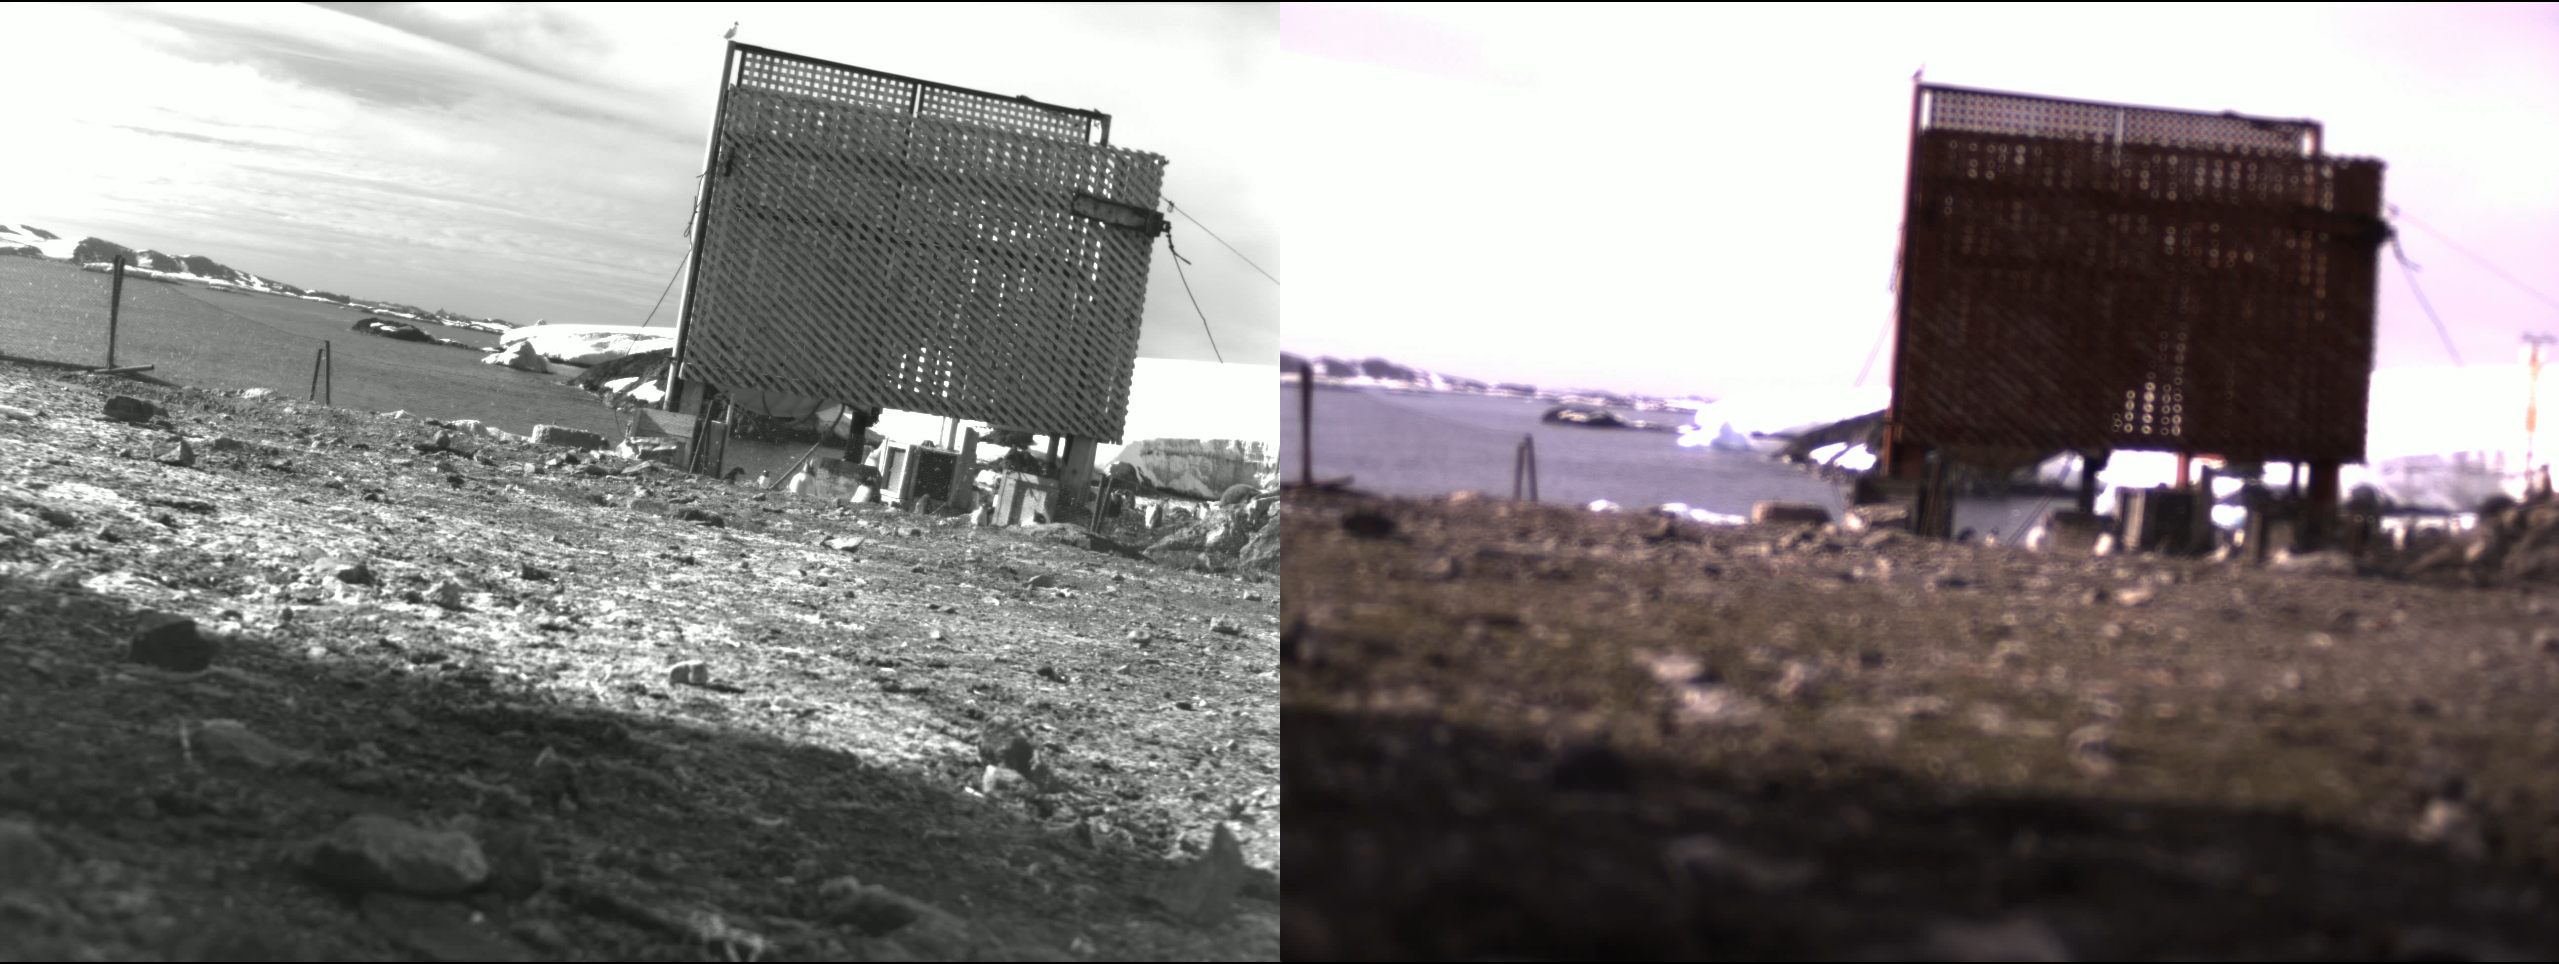
\includegraphics[width=1\textwidth]{Figures/C4/pinguinos.png}
    \caption{Captura de video realizada exitosamente durante la expedición científica en la Antártida. La imagen confirma que, a pesar de las condiciones extremas, el sistema \textit{QBee} En la imagen se aprecia que la cámara visible no se encuentra correctamente enfocada, lo que puede deberse a un mal ajuste de la distancia entre el objetivo y el sensor. Sin embargo, este tipo de desajuste es corregible mediante ajuste mecánico y no afecta el funcionamiento general del sistema \textit{QBee}. fue capaz de operar y registrar datos multiespectrales de forma puntual.}
    \label{fig:prueba_antartida}
    \end{figure}

    \subsubsection{Pruebas en vuelo}

    Las pruebas en vuelo del sistema \textit{QBee} fueron posibles gracias a la colaboraci'on con la Fuerza A'erea Colombiana, la cual facilit'o el montaje del dispositivo en distintas aeronaves de su flota. En una primera prueba, la unidad \textit{QBee} fue instalada a bordo de una aeronave Cessna 208 Caravan, realizando un vuelo a una altitud aproximada de 5000 pies.
    
    \noindent El vuelo se desarroll'o en condiciones ideales, con un rumbo y comportamiento t'ipico de una ruta comercial y sin presencia de perturbaciones atmosf'ericas significativas. Durante toda la duraci'on del trayecto, el sistema oper'o de forma estable y sin presentar inconvenientes.
    
    \noindent Como parte de esta prueba, se verific'o la capacidad de monitoreo remoto del sistema utilizando una red Wi-Fi habilitada dentro de la aeronave, mediante la cual se accedi'o al entorno gr'afico de la Raspberry Pi utilizando el protocolo VNC. Esta conexi'on permiti'o observar en tiempo real la adquisici'on de datos por parte del sistema, confirmando la funcionalidad completa del script y la respuesta de los sensores.
    
    \begin{figure}[!h]
    \centering
    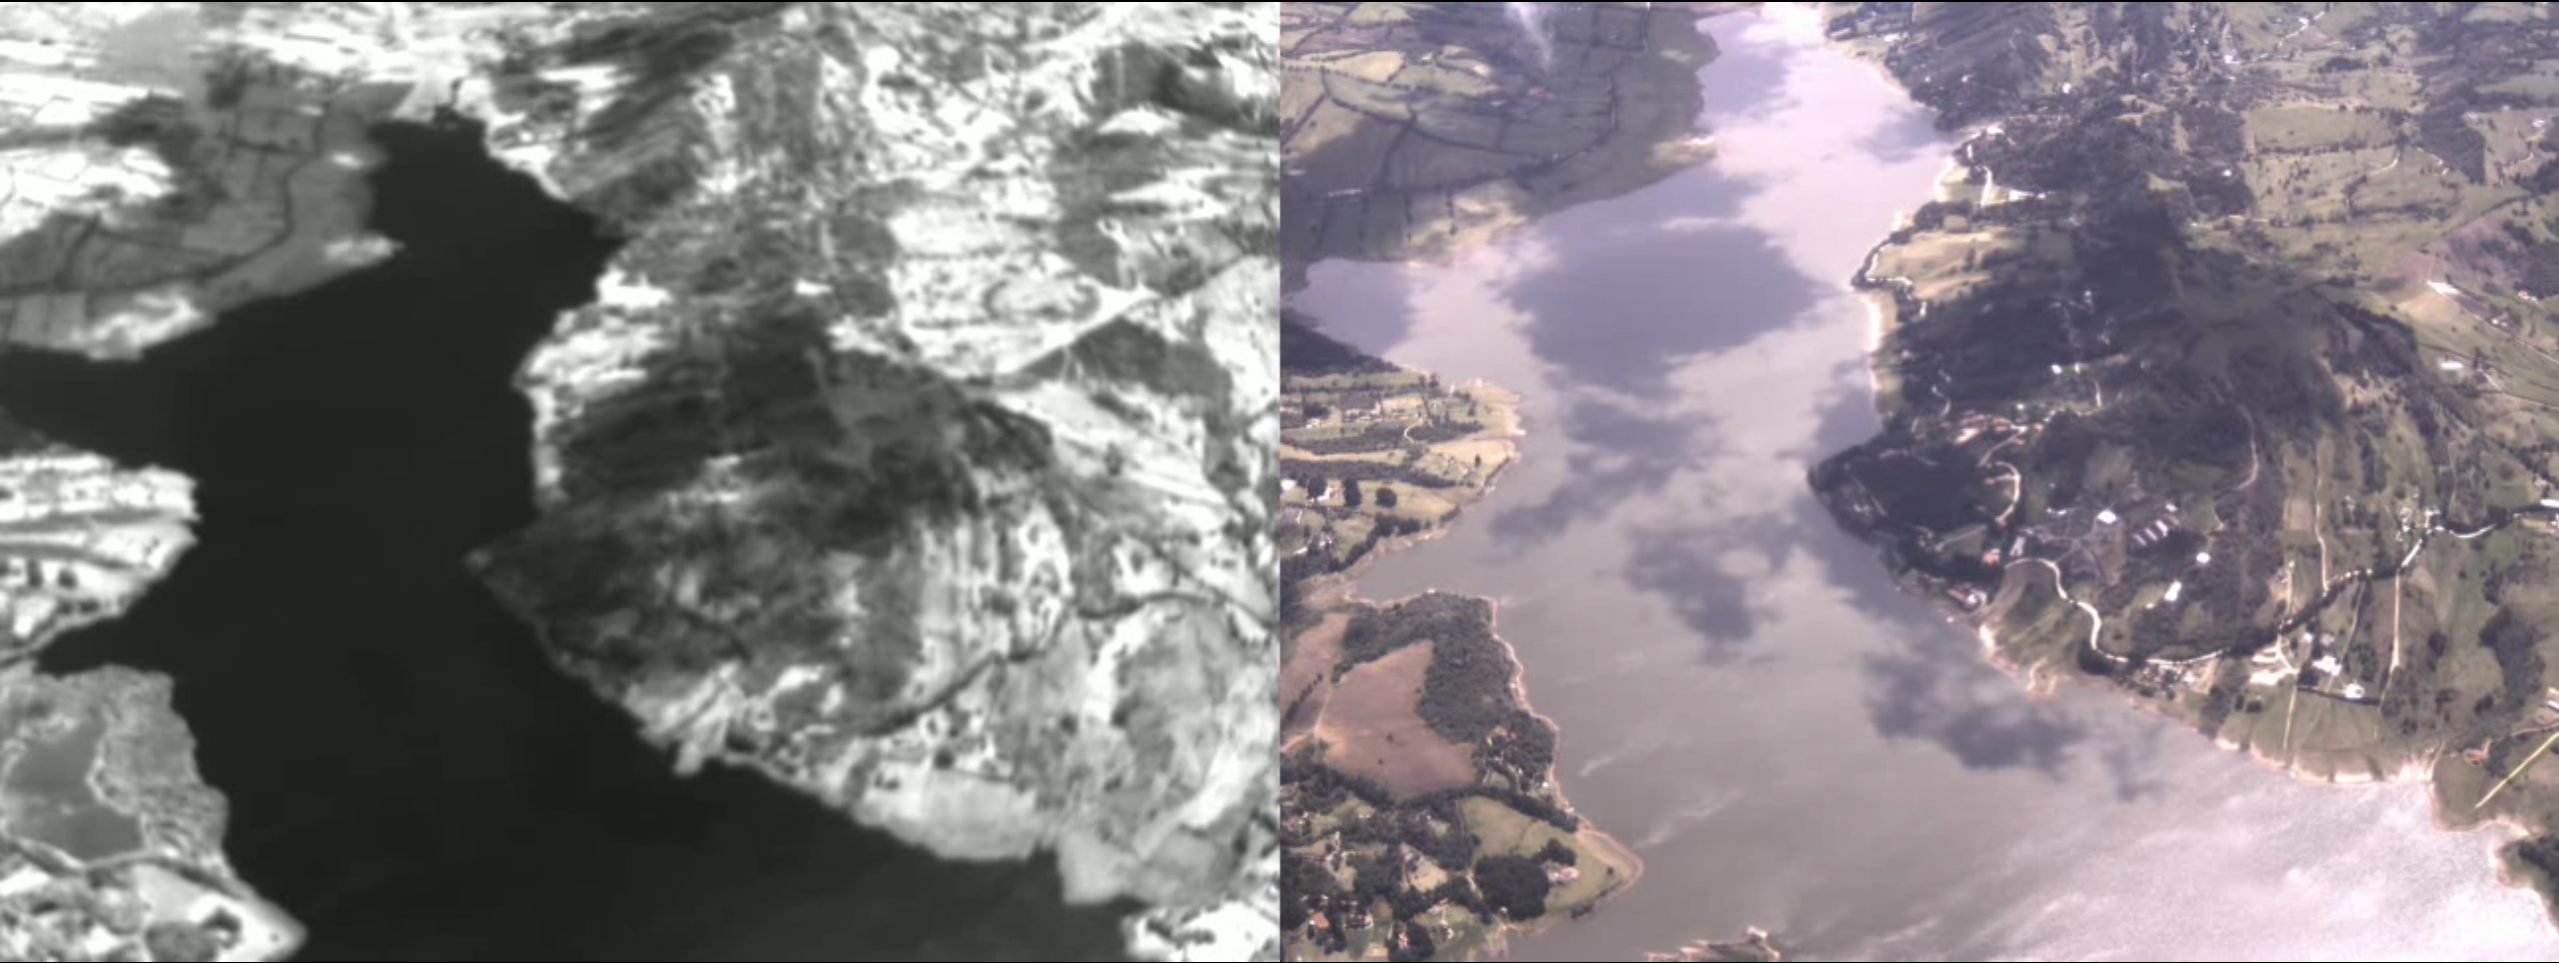
\includegraphics[width=1\textwidth]{Figures/C4/vuelo_caravan.png}
    \caption{Captura tomada durante el vuelo de prueba en la aeronave Cessna 208 Caravan. Se observ'o un comportamiento estable del sistema y transmisi'on remota exitosa mediante protocolo VNC.}
    \label{fig:prueba_vuelo}
    \end{figure}

    \noindent En una segunda prueba, la unidad \textit{QBee} fue montada a bordo de una aeronave de combate Tucano T-27, con el fin de validar su desempeño bajo condiciones de vuelo más exigentes. En este caso, no se contó con un sistema de monitoreo en tiempo real debido a las restricciones propias de la aeronave. Sin embargo, el sistema operó de forma autónoma durante la misión, registrando exitosamente la captura de video.

    \noindent A diferencia del vuelo en la Cessna Caravan, esta prueba presentó una complejidad adicional, ya que durante la operación se ejecutaron maniobras que alcanzaron aceleraciones de hasta 4g. A pesar de estas condiciones dinámicas, la \textit{QBee} logró completar su función de adquisición sin incidentes, lo cual representa un resultado relevante sobre la robustez mecánica y operativa del sistema.
    
    \begin{figure}[!h]
    \centering
    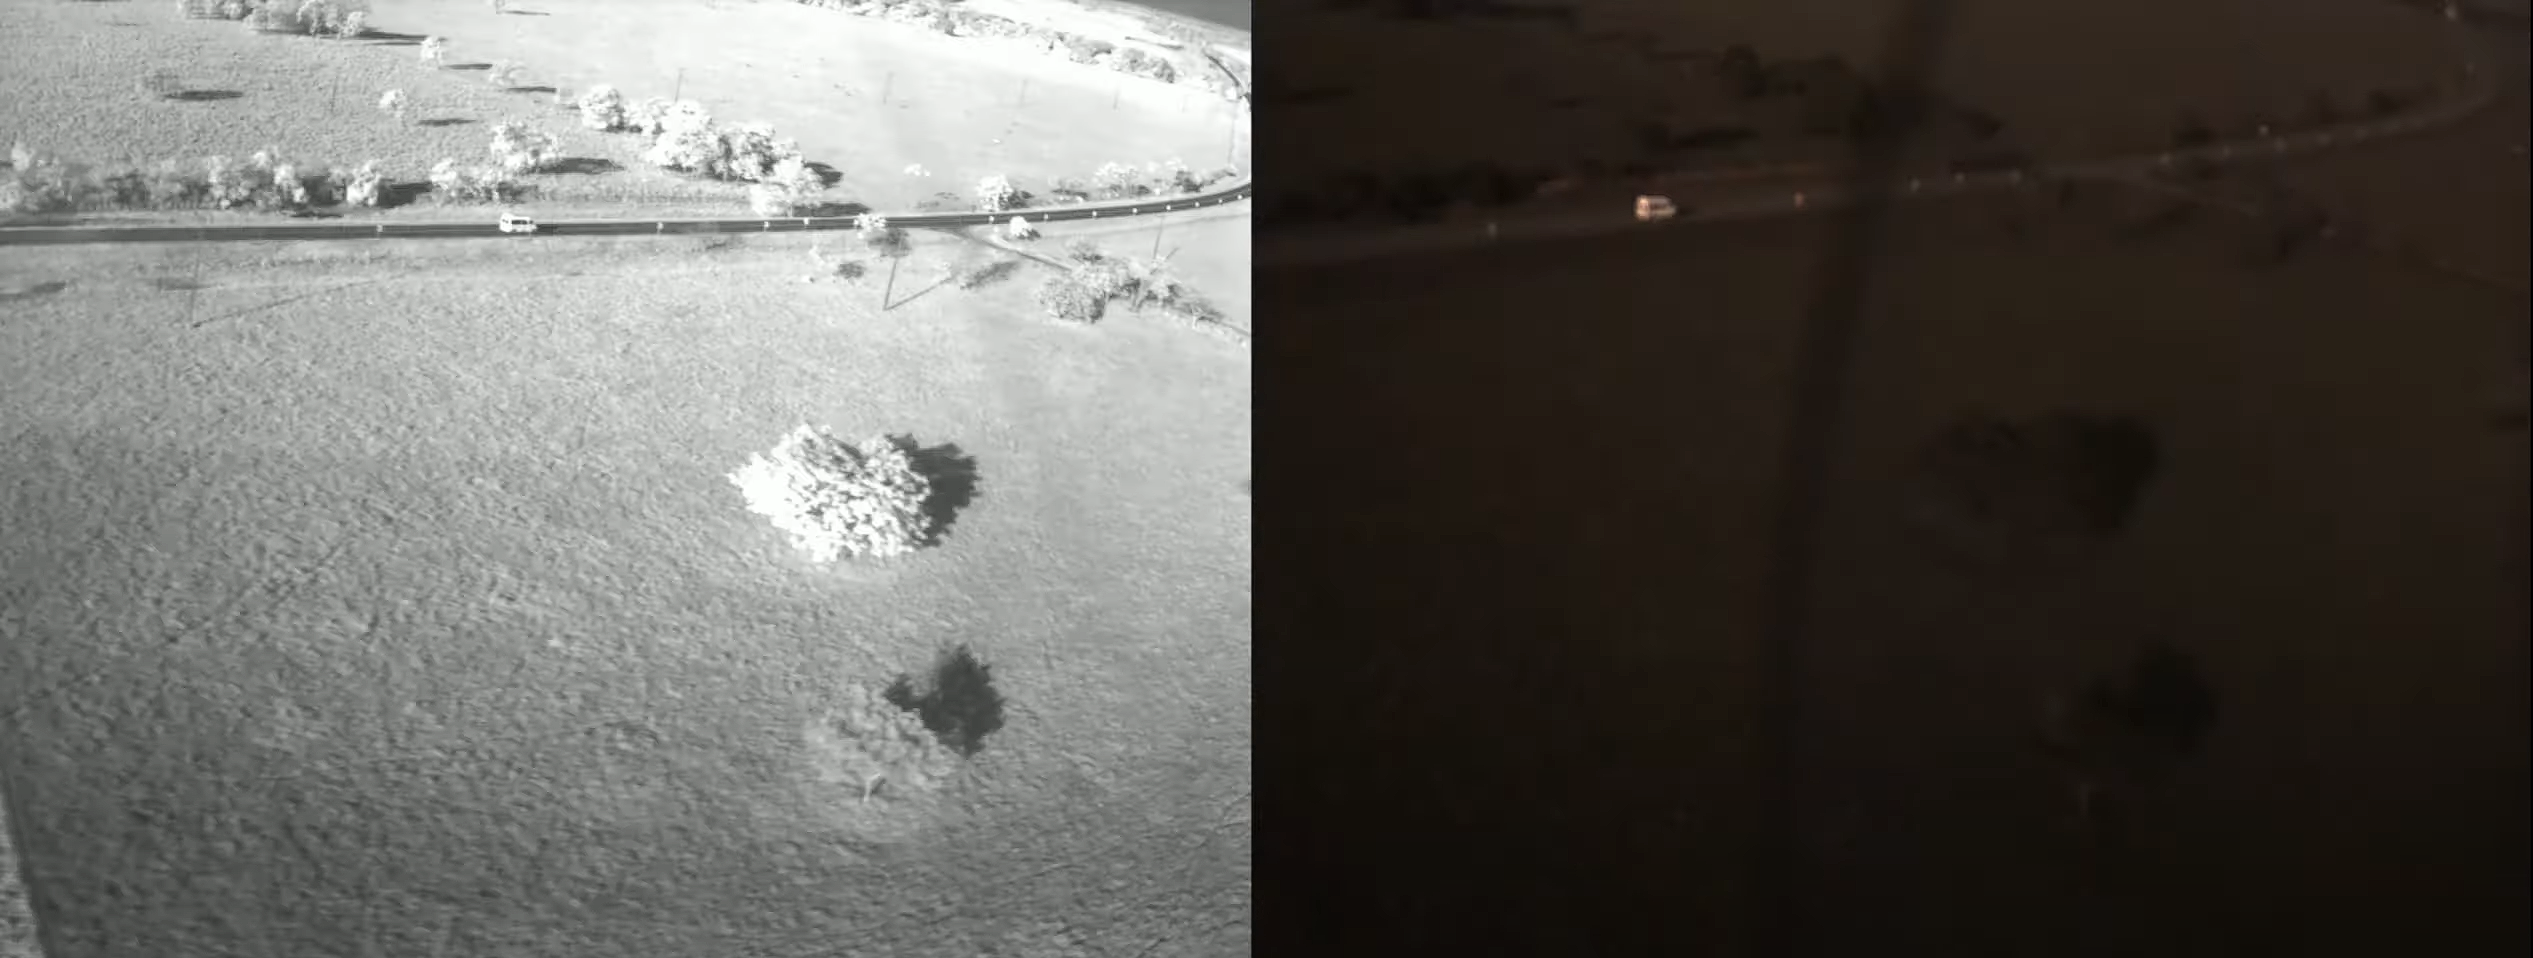
\includegraphics[width=0.9\textwidth]{Figures/C4/t2.png}
    \caption{Captura de video realizada durante prueba a bordo del avión de combate T-27 Tucano. A pesar de las maniobras con aceleraciones de hasta 4g, el sistema \textit{QBee} logró registrar imágenes de forma autónoma y estable. Las condiciones de iluminación ambiental no erán las más adecuadas debido a la hora del día (proximadamente las 6 pm).}
    \label{fig:prueba_tucano}
    \end{figure}

    \section{Conclusiones y lecciones aprendidas}

    temperatura, la saturacion, la cita de velocidad, los links a los videos, sobre el codigo, 
\chapter{Results \& Discussion}         % o \chapter{Resultados y Discusión}

%===============================================================
\section{Diseño del sistema multiespectral \textit{KBee}}
%===============================================================

La ruta de desarrollo del \textit{KBee} partió de una matriz de ocho “sistemas   candidatos’’ (Apendice \ref{ap:sistemas_candidatos}); de ellos se seleccionaron las dos configuraciones VIS + NIR que mejor satisfacen las restricciones de misión impuestas por el consorcio
EAFIT–KTH: altura de operación $50$–$5\,000\;{\rm m}$, peso $\leq$ $2\;{\rm kg}$,
envolvente geométrica $100\times100\times150\;{\rm mm}^{3}$ y conectividad USB 3.1.
A continuación se describe el hilo de razonamiento que condujo al diseño final.

%---------------------------------------------------------------
\subsection{Requerimientos y criterios ópticos}
%---------------------------------------------------------------

\begin{table}[h]
    \centering
    \caption{Especificaciones de misión y criterios de diseño del \textit{KBee}.}
    \label{tab:req_vs_obj}
    \begin{tabular}{|p{4cm}|c|}
        \hline
        \rowcolor[HTML]{EFEFEF}\textbf{Parámetro} & \textbf{Requisito} \\ \hline
        Masa total del cargamento & $\leq 2\;\text{kg}$ \\ \hline
        Dimensiones & $100 \times 100 \times 150\;\text{mm}^{3}$ \\ \hline
        Tiempo máximo de misión & $\leq 3\;\text{h}$ \\ \hline
        MTF (30\,\% de contraste) & $\geq 40\;\text{lp/mm}$ \\ \hline
        Resolución en tierra @50\,m & $\leq 7.35\;\text{cm}$ \\ \hline
        Resolución en tierra @1000\,m & $\leq 1.47\;\text{m}$ \\ \hline
        Resolución en tierra @5000\,m & $\leq 7.35\;\text{m}$ \\ \hline
    \end{tabular}
\end{table}


Los criterios que guiaron la selección de cada sub‑módulo fueron:

\begin{itemize}
    \item \textbf{Resolución espacial} – El objetivo debe ofrecer una MTF (30\,\% de contraste) 
          \textbf{$\geq 40\;\text{lp/mm}$}, lo que garantiza la capacidad de resolver los objetos 
          de las dimensiones indicadas en la Tabla~\ref{tab:req_vs_obj}.
          
    \item \textbf{Campo de visión} – El ángulo AFOV debe cubrir parcelas agrícolas 
          de al menos 50 m a baja altura sin comprometer la resolución a grandes altitudes; 
          por ello se seleccionan dos distancias focales representativas: 
          8 mm (NIR) y 16 mm (VIS).
          
    \item \textbf{Masa y volumen} – El conjunto óptico‑electrónico debe cumplir las 
          restricciones de carga útil de la aeronave del Proyecto C\#, 
          de modo que se mantenga un tiempo de vuelo de 3 h.  
          En la práctica esto implica una masa total $\leq 2\;\text{kg}$ 
          y un volumen aproximado de $100\times100\times150\;\text{mm}^{3}$.
          
    \item \textbf{Coste} – Aunque el presupuesto final depende de los fondos del proyecto, 
          para este trabajo se fija un \emph{límite máximo de \$1500 USD}.  
          Con un presupuesto mayor podrían integrarse componentes de mayor rendimiento.
\end{itemize}


%---------------------------------------------------------------
\subsection{Proceso iterativo de diseño}
\label{sec:cad}
%---------------------------------------------------------------

La Tabla~\ref{tab:sys_tables} resume los ocho objetivos evaluados de
forma preliminar.  Cada sistema se identifica por un número consecutivo y se
caracteriza mediante distancia focal, relación de apertura, MTF al 30\,\% de
contraste y masa total del objetivo.

\begin{table}[h]
    \centering
    \caption{Comparativa de los objetivos candidatos frente a los criterios de diseño.
             Entre paréntesis se indica el fabricante (EO = Edmund Optics).  El AFOV
             se expresa en grados y corresponde al semidiámetro angular calculado
             sobre el sensor empleado.}
    \label{tab:sys_tables}
    \begin{tabularx}{\linewidth}{|c|p{3cm}|C|C|C|C|C|}
        \hline
        \rowcolor[HTML]{EFEFEF}\textbf{System} & \textbf{Lens} &
        \textbf{Focal\, [mm]} &
        \textbf{AFOV\, [°]} &
        \textbf{Aperture} &
        \textbf{MTF\,(30 \%)\, [lp/mm]} &
        \textbf{Weight\, [g]} \\ \hline
        
        1 & 16 mm f/16 ― HPr Series (EO)                & 16   & 42.2 & f/16 & 62  & 138 \\ \hline
        2 & 50 mm f/2.8 ― HPr Series (EO)               & 50   & 10.1 & f/2.8& 180 & --  \\ \hline
        3 & 25 mm f/1.8 ― HPr Series (EO)               & 25   & 27.8 & f/1.8& 40  & 78  \\ \hline
        4 & 16 mm f/1.8 ― HPr Series (EO)               & 16   & 42.2 & f/1.8& 128 & 138 \\ \hline
        5 & 4 mm f/1.8 ― Basler C125‑0418‑5M‑P (Basler) & 4    & 109  & f/1.8& --  & --  \\ \hline
        6 & 8 mm f/2.5 ― HEO Series (NIR, M12) (EO)     & 8    & 29.9 & f/2.5& 120 & 4   \\ \hline
        7 & 8.5 mm f/1.3 ― Cr Series (EO)               & 8.5  & 28.2 & f/1.8& 85  & 60  \\ \hline
        8 & 12.5 mm f/2.5 ― Rugged Blue (M12) (EO)      & 12.5 & 19.4 & f/2.5& 150 & 5   \\ \hline
    \end{tabularx}
\end{table}


La resolución exigida (MTF $\geq40\,$lp mm\(^{-1}\)) se cumple de forma holgada en
los sistemas 2, 4, 6, 7 y 8.  El sistema 2, con 50 mm f/2.8, ofrece la mayor
frecuencia de corte (180 lp mm\(^{-1}\)), lo que se traduce en la más alta
resolución sobre el terreno; sin embargo, su AFOV es el más estrecho del
conjunto, limitando el área cubierta por captura.  En el extremo opuesto, el
objetivo de 4 mm (sistema 5) maximiza el AFOV —casi \(110^{\circ}\) en sensor
arrectángulo— pero carece de datos MTF publicados y podría no satisfacer la
resolución mínima.  Las configuraciones de 8 mm f/2.5 (sistema 6) y
8.5 mm f/1.8 (sistema 7) constituyen un compromiso atractivo: mantienen AFOV
moderado ($\approx60^{\circ}$), cumplen la MTF requerida y añaden la banda NIR
(NIR–M12) con una masa inferior a 60 g, adecuada para misiones de baja y media
altitud.\\

En sistemas aéreos que operan a distancias de decenas o miles de metros, el
plano de enfoque se aproxima al infinito; el sistema trabaja, por tanto, en
régimen de hiperfoco y la profundidad de campo deja de ser un factor
limitante.  No obstante, la apertura \((f/\#)\) sigue siendo relevante porque
regula la cantidad de luz incidente y la eficiencia con la que se reproducen
las altas frecuencias espaciales.  Los objetivos de gran abertura
(f/1.8–f/2.5) —sistemas 3, 4, 6, 7 y 8— captan hasta dos pasos más de luz que
el objetivo f/16 (sistema 1), mejorando la SNR de la imagen y preservando la
modulación a altas frecuencias del MTF.\\

El límite de carga útil de la plataforma \textit{C3} es 2 kg para lograr un tiempo de vuelo de 3 h. Aunque todos los objetivos de la Tabla \ref{tab:sys_tables} se encuentran muy por debajo de ese umbral, los sistemas 6, 7 y 8 destacan por su masa extraordinariamente baja (entre 4 g y 60 g), lo que los convierte en las opciones más atractivas cuando el peso es el factor decisivo. En la etapa de prototipado se dará prioridad a estas configuraciones ligeras, siempre que satisfagan además el requisito mínimo de resolución.


Los sistemas 6 (NIR 8 mm f/2.5) y 7 (VIS 8.5 mm f/1.8) aparecen
como las mejores combinaciones de AFOV, MTF y peso para vuelos de 50–1000 m,
mientras que el sistema 2 (50 mm f/2.8) se reserva para misiones de gran
altitud donde se privilegia la resolución sobre la cobertura espacial.\\




---------------------------------------------------------------
\subsection{Pre‑selección de sensores de imagen}
\label{sec:sensor_selection}
%---------------------------------------------------------------
Para cada sistema óptico se evaluaron seis configuraciones de cámara
(Alvium/Basler) representativas de los rangos de resolución y tamaño de píxel
requeridos.  En la Tabla~\ref{tab:sensor_table} se recogen únicamente los
parámetros que afectan de forma directa al diseño de la carga y al cálculo de
resolución: peso, profundidad de bits, tipo de obturación
(\textit{rolling}/\textit{global}), tamaño del sensor, tamaño de píxel y
consumo energético típico.

\begin{table}[h]
    \centering
    \caption{Sensores propuestos, su asignación a los sistemas ópticos y parámetros clave.}
    \label{tab:sensor_table}
    \begin{tabularx}{\linewidth}{|c|p{2.2cm}|C|C|C|C|C|C|}
        \hline
        \rowcolor[HTML]{EFEFEF}
        \textbf{Sistema} &
        \textbf{Cámara (sensor)} &
        \textbf{H\,$\times$\,V [px]} &
        \textbf{Pixel [\(\mu\)m]} &
        \textbf{Shutter} &
        \textbf{ADC / Bits} &
        \textbf{Peso [g]} &
        \textbf{Potencia [W]} \\ 
        \hline

        1, 3, 4 & Alvium 1800 U‑2040 (Sony IMX541)            & 4512 × 4512 & 2.74 & Global  & 12 bit & 65 & 3.9 \\ \hline
        2  & Alvium 1800 U‑2050 (Sony IMX183)            & 5496 × 3672 & 2.40 & Rolling & 10 bit & 65 & 3.2 \\ \hline
        5 & Basler acA1920‑40gc (Sony IMX249)           & 1920 × 1200 & 5.86 & Global  & 12 bit & 90 & 3.9 \\ \hline
        6 & Alvium 1800 U‑501m NIR (ON Semi AR0522)     & 2592 × 1944 & 2.20 & Rolling & 10 bit & 65 & 2.2 \\ \hline
        7, 8 & Alvium 1800 U‑500c (ON Semi AR0521, C, S‑Mount)& 2592 × 1944 & 2.20 & Rolling & 10 bit & 60 & 2.2 \\ \hline
        
    \end{tabularx}
\end{table}

\noindent Todos los sensores considerados pesan menos de 100 g y consumen por debajo de 4 W. En particular, los basados en los CCD ON Semi AR0521 / AR0522 (sistemas 6–8) son los más ligeros (60–65 g) y presentan el consumo más bajo ($\approx$ 2.2 W), lo que resulta clave para maximizar la autonomía de vuelo de la plataforma \textit{C3}.\\

\noindent Para garantizar un buen análisis radiométrico, es necesario contar con al menos 10 bits de conversión A/D. Los sensores Sony IMX541 e IMX249 ofrecen hasta 12 bits y disponen de obturación global, lo que evita distorsiones ante movimientos rápidos o flashes de luz. Por otro lado, los módulos AR0521 / AR0522 con obturación \emph{rolling} son considerablemente más económicos, ayudando a mantener los costos reducidos; sin embargo, en maniobras o al capturar objetos en movimiento pueden aparecer artefactos por el desplazamiento relativo durante la lectura línea a línea.\\

\noindent El tamaño de píxel condiciona directamente la resolución espacial. Los sensores con celdas de 2.2–2.74 µm (IMX541, IMX183, AR05xx) se adaptan a los objetivos de alta resolución (sistemas 1–4, 6–8); el IMX249, con 5.86 µm, es idóneo para configuraciones de campo muy amplio (sistema 5), donde prima la sensibilidad sobre la densidad de píxel.\\

\noindent Teniendo en cuenta masa, consumo, profundidad de bits y tamaño de píxel, junto con los resultados de la Tabla~\ref{tab:sensor_table}, proponemos como configuración óptima la pareja AR0521 (VIS) + AR0522 (NIR) montada en lentes de 8.5 mm f/1.8 y 8 mm f/2.5 (sistemas 7 y 6). Esta combinación ofrece un equilibrio ideal entre resolución, campo de visión y eficiencia energética para las misiones del proyecto \textit{C3}.\\

\noindent Con estas combinaciones se logra un balance adecuado entre resolución, peso y consumo, ajustado al presupuesto y a las exigencias operativas de la plataforma.

%---------------------------------------------------------------
\subsection{Estimación teórica de resolución y campo de visión}
\label{sec:cad_sim}
%---------------------------------------------------------------

Para cuantificar el compromiso entre resolución y cobertura se simularon ocho
trenes ópticos (lentes de la Tabla \ref{tab:sys_tables}) a tres alturas de
operación: 50 m (vuelo bajo), 1000 m (vuelo medio) y 5000 m (vuelo alto). En la Tabla~\ref{tab:grd_fov_clean} se presentan, para cada sistema óptico y a tres alturas de vuelo, el campo de visión efectivo sobre el terreno (FOV), la magnificación primaria, la resolución limitada solo por el paso de píxel (\(\Delta_{\mathrm{pix}}\)) y la resolución real impuesta por la óptica a MTF 30\,\% (\(\Delta_{\mathrm{MTF}}\)).\\


\begin{table}[h]
    \centering
    \footnotesize
    \setlength{\tabcolsep}{6pt}
    \caption{Field‑of‑view (FOV), magnification and ground resolution 
             (\(\Delta_\text{pix}\), \(\Delta_\text{MTF}\)) for each system
             at three altitudes.}
    \label{tab:grd_fov_clean}
    \begin{tabular}{|c|c|c|c|c|c|}
        \hline
        \rowcolor[HTML]{EFEFEF}
        \textbf{System} & \textbf{Alt [m]} & \textbf{FOV [m]} & 
        \textbf{Magn.} & \(\boldsymbol{\Delta_\text{pix}}\)\,[m] & 
        \(\boldsymbol{\Delta_\text{MTF}}\)\,[m] \\ 
        \hline
        
        \multirow{3}{*}{1} 
         & 50   & 38.63  & 0.00032   & 0.00860  & 0.02500   \\ 
         & 1000 & 772.70 & 0.00002   & 0.17100  & 0.50400   \\ 
         & 5000 & 3863.00& 0.00000   & 0.85600  & 2.52000   \\ 
        \hline
        
        \multirow{3}{*}{2}
         & 50   & 8.81   & 0.00150   & 0.00160  & 0.00190  \\ 
         & 1000 & 176.30 & 0.00008   & 0.03200  & 0.03700   \\ 
         & 5000 & 881.30 & 0.00002   & 0.16000  & 0.18600   \\ 
        \hline
        
        \multirow{3}{*}{3}
         & 50   & 24.73  & 0.00050   & 0.00548  & 0.02500   \\ 
         & 1000 & 494.50 & 0.00003   & 0.11000  & 0.50000   \\ 
         & 5000 & 2473.00& 0.00001   & 0.54800  & 2.50000   \\ 
        \hline
        
        \multirow{3}{*}{4}
         & 50   & 38.63  & 0.00032   & 0.00860  & 0.01200   \\ 
         & 1000 & 772.70 & 0.00002   & 0.17100  & 0.24400   \\ 
         & 5000 & 3863.00& 0.00000   & 0.85600  & 1.22100   \\ 
        \hline
        
        \multirow{3}{*}{5}
         & 50   & 140.60 & 0.00005   & 0.11700  & —         \\ 
         & 1000 & 2812.80& 0.00000   & 2.34400  & —         \\ 
         & 5000 & 14064.00&0.00000   & 11.72000 & —         \\ 
        \hline
        
        \multirow{3}{*}{6}
         & 50   & 26.73  & 0.00021   & 0.01030  & 0.01900   \\ 
         & 1000 & 534.60 & 0.00001   & 0.20600  & 0.39100   \\ 
         & 5000 & 2673.00& 0.00000   & 1.03100  & 1.95300   \\ 
        \hline
        
        \multirow{3}{*}{7}
         & 50   & 25.16  & 0.00017   & 0.01290  & 0.03400   \\ 
         & 1000 & 503.20 & 0.00001   & 0.25900  & 0.69200   \\ 
         & 5000 & 2516.00& 0.00000   & 1.29400  & 3.46000   \\ 
        \hline
        
        \multirow{3}{*}{8}
         & 50   & 17.11  & 0.00025   & 0.00880  & 0.01300   \\ 
         & 1000 & 342.10 & 0.00001   & 0.17600  & 0.26700   \\ 
         & 5000 & 1711.00& 0.00000   & 0.88000  & 1.33300   \\ 
        \hline
    \end{tabular}
\end{table}




\noindent A simple vista, \(\Delta_{\mathrm{MTF}}\) resulta siempre mayor que \(\Delta_{\mathrm{pix}}\), lo cual era de esperar: la óptica atenúa las altas frecuencias y limita un poco el detalle que el sensor podría capturar de forma ideal. Este hallazgo confirma que se ha elegido sensores con tamaño de píxel suficiente para no desaprovechar la capacidad de resolución de las lentes.\\

\noindent En cuanto al equilibrio entre cobertura y nitidez, los sistemas de focal larga concentran cada píxel en un área reducida —mejor nitidez— pero limitan mucho la zona capturada. En el otro extremo, los de focal muy corta expanden enormemente el FOV a costa de degradar la resolución. Los sistemas 6 (8 mm f/2.5, NIR) y 7 (8.5 mm f/1.8, VIS) aparecen como el compromiso ideal: a 50 m cubren unos 26 m de ancho con \(\Delta_{\mathrm{MTF}}<1.5\)\,cm, y a 1000 m mantienen resoluciones de 20 – 26 cm sobre aproximadamente 500 m de cobertura.\\

\noindent Además, al compartir casi la misma geometría óptica, facilitan la fusión multiespectral y minimizan desalineamientos entre canales. Por estas razones, para el prototipo inicial daremos prioridad a los sistemas 6 y 7, que combinan de forma natural cobertura, detalle y compatibilidad espectral.\\


\section{Construcción e integración del prototipo}
  \subsection{Modelo CAD y ensamblaje mecánico}
    % → FIGURA grande: render CAD explosionado del KBee con leyenda de partes.
    %   Tabla: materiales y masa de cada componente.

    \begin{figure}[h]
        \centering
        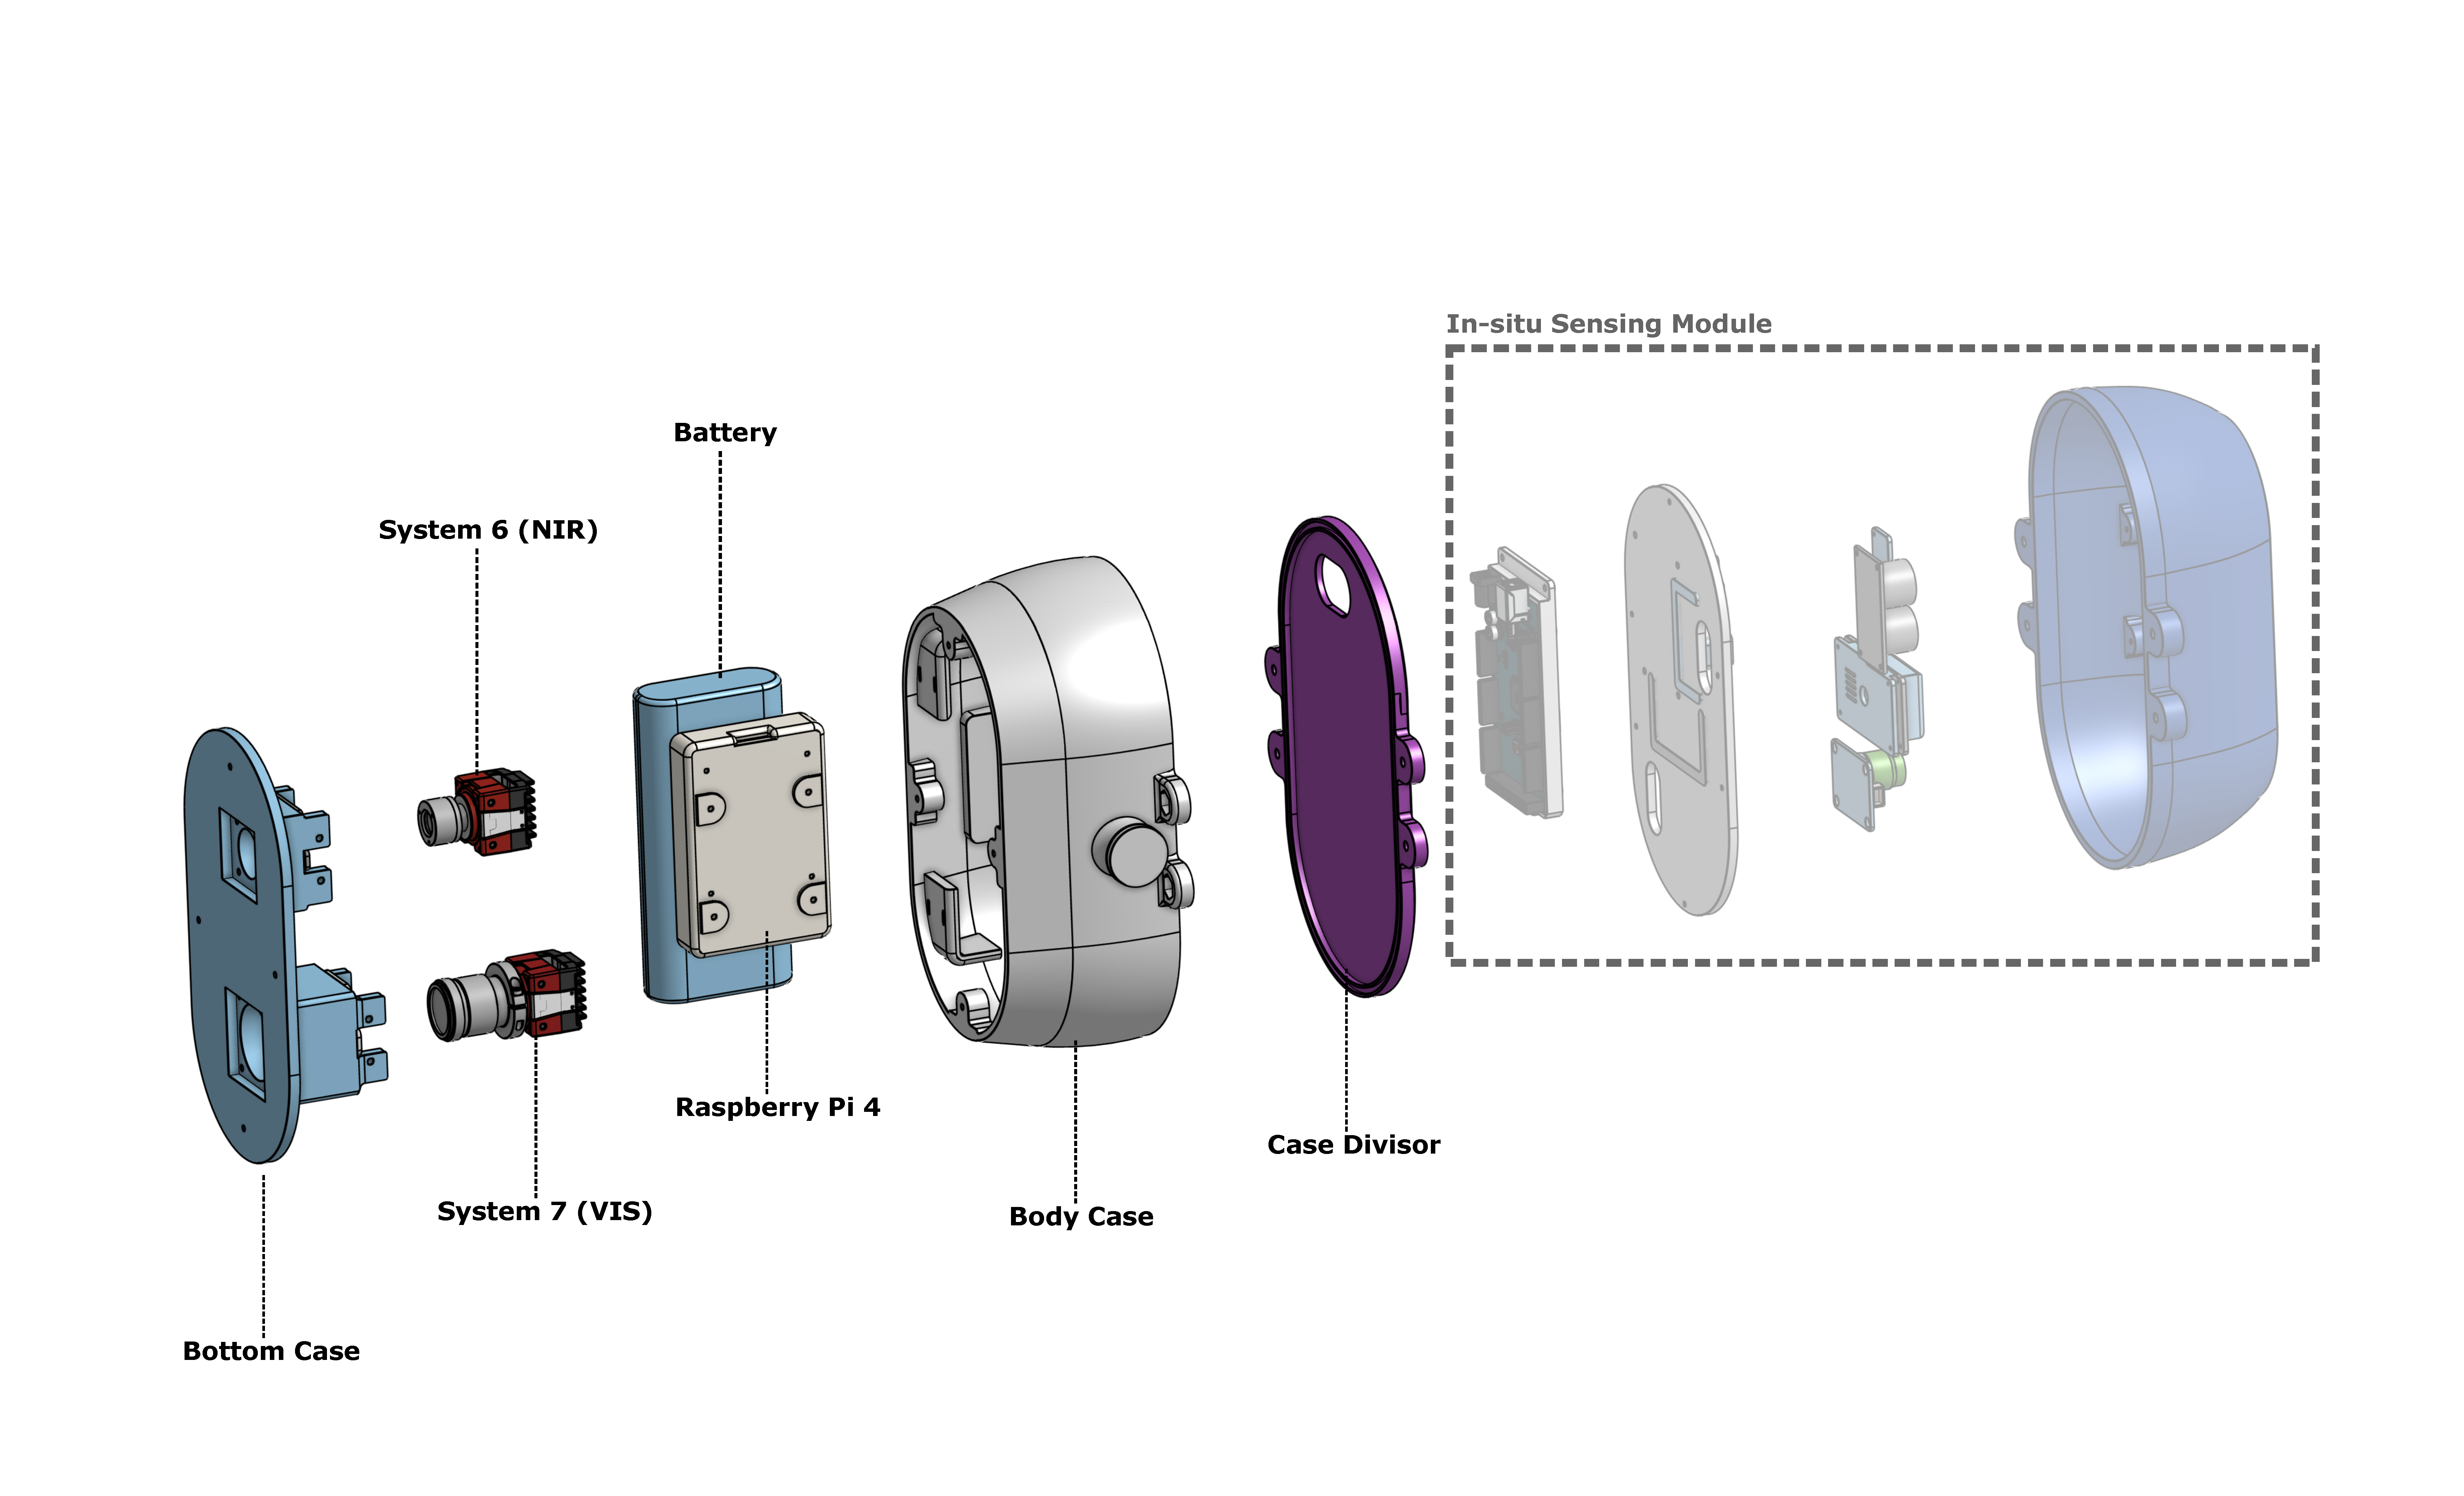
\includegraphics[width=1\linewidth]{Figures/C4/QBee.pdf}
        \caption{Vista explosionada del ensamble completo del QBee, mostrando la carcasa impresa en PET‑G y la disposición de los sistemas 6 (NIR, 8 mm f/2.5) y 7 (VIS, 8.5 mm f/1.8). Este diseño y construcción fue concebido con el apoyo del equipo de manufactura del pryecto C3.}
        \label{fig:exploded_assembly}
    \end{figure}

    El case del QBee está impreso en PET‑G (tereftalato de polietileno modificado con glicol), un polímero cuya densidad típica ronda 1,317 g/cm³, que combina buena resistencia al impacto (Charpy $\approx$ 4,03 kJ/m²) y alargamiento al rompimiento hasta 15\% en formulaciones estándar. Su módulo de tracción (~4015 MPa) y de flexión (~2987 MPa) aseguran rigidez, mientras que su temperatura de transición vítrea ($\approx$ 76 °C) y rango de fusión (220–260 °C) lo hacen estable en el calor generado por electrónica cercana. Además, presenta excelente durabilidad química y mínima tendencia al \emph{warping}, ideal para piezas de geometría compleja. El peso total del disposito es de 1.810 gramos, cumpliendo así con el requisito de peso impuesto.\\

    \noindent La dimensión externa del case se diseñó para encajar en el bay interno del UAV C3, sin requerir hermeticidad, ya que este estária protegido de las condiciones exteriores. El cierre se logra con tornillos M3 que unen la tapa inferior y el divisor de compartimentos a la carcasa principal. En el interior, cada sistema óptico (6/NIR y 7/VIS) se ancla directamente al sensor mediante cuatro tornillos M3 en sus laterales, asegurando alineación con el eje de vuelo. El sistema 6 (NIR) monta el Alvium 1800 U‑501m (AR0522) + objetivo 8 mm f/2.5 + filtro 850 nm en montura S, todo encapsulado en una montura de resina 3D. El sistema 7 (VIS) agrupa el Alvium 1800 U‑500c (AR0521) + objetivo 8.5 mm f/1.3 ruggedized + filtro VIS UV/IR Cut en rosca M25.5, manteniendo rigidez frente a vibraciones.\\
    
    \noindent La unidad de cómputo y almacenamiento es una Raspberry Pi 4, colocada en un bloque intermedio y alimentada por una powerbank de 20.000 mAh. Este sistema tiene acoplado un hat de GPS, que suministra al sistema de metadatos de fecha, hora UTC, latitud, longitud, altitud y ángulo de elevación, esenciales para la georreferenciación y ortorrestitución de imágenes. Finalmente, el módulo in situ de sensado de contaminantes comparte alimentación de 5 V de la misma batería y ocupa el compartimento trasero de la carcasa, completando la funcionalidad del QBee.\\
    
    



    \noindent Los sistemas 6 y 7 integran un sensor, un objetivo y un filtro específicos montados sobre la carcasa impresa (Figura~\ref{fig:exploded_assembly}). Esta configuración facilita la fabricación y el mantenimiento, y permite intercambiar o actualizar componentes de forma independiente.\\

    \noindent El sensor NIR Allied Vision Alvium 1800 U‑501m (ON Semi AR0522) comparte tamaño de sensor (2592×1944 px) y paso de píxel (2.2 µm) con su homólogo VIS, pero presenta una respuesta cuántica optimizada en 700–1000 nm, ideal para la adquisición de imagenes en este rango espectral. El objetivo HEO Series de 8 mm f/2.5 se monta directamente sobre la montura S‑Mount y ofrece un AFOV de 29.9°. Con 4 g de masa, cumple el requisito de carga útil y minimiza la transmisión de vibraciones. La montura impresa en resina aloja un filtro paso banda de 850 \SI{}{nm} (CWL) y 50 \SI{}{nm} de ancho de banda, 12.5 mm de diámetro, Hard Coated OD 4.0, encajando sobre el barril y fijándose con un anillo roscado que garantiza la alineación sin sobresalir del perfil de la carcasa.\\
    
    \noindent El sensor VIS Alvium 1800 U‑500c (ON Semi AR0521) mantiene los 2.2 µm de paso de píxel y emplea obturación rolling, reduciendo peso y costo. El objetivo Cr Series de 8.5 mm f/1.3, ruggedized por el fabricante, ofrece gran apertura y resistencia a impactos y vibraciones.. El filtro VIS (UV/IR Cut) M25.5×0.50 bloquea 200–370 nm y 750 – 1100 nm, transmitiendo solo 370–750 nm, e integra directamente una montura compatible para el montaje en el objetivo.\\
    
    \noindent La conectividad micro USB‑B facilita la alimentación y transmisión de datos con la Raspberry Pi 4 (Figura~\ref{fig:sistemas_opticos_componentes}). Además, permiten la integración y control de los sensores a partir de un script en python, lo cual da flexibilidad para diseñar el preprocesamiento y captura de las imágenes de ambos sensores de forma simultanea. Esto permite incluso carga confirguracones ya establecidas o actauliza en tiempo real dichas fongiruaciones relacioandas a paramaetros como, por ejemplo, el tiempo de exposiicón o la ganancia.
    
        
    
    
    
    


    \begin{figure}[h]
        \centering
        \begin{subfigure}[b]{0.48\linewidth}
            \centering
            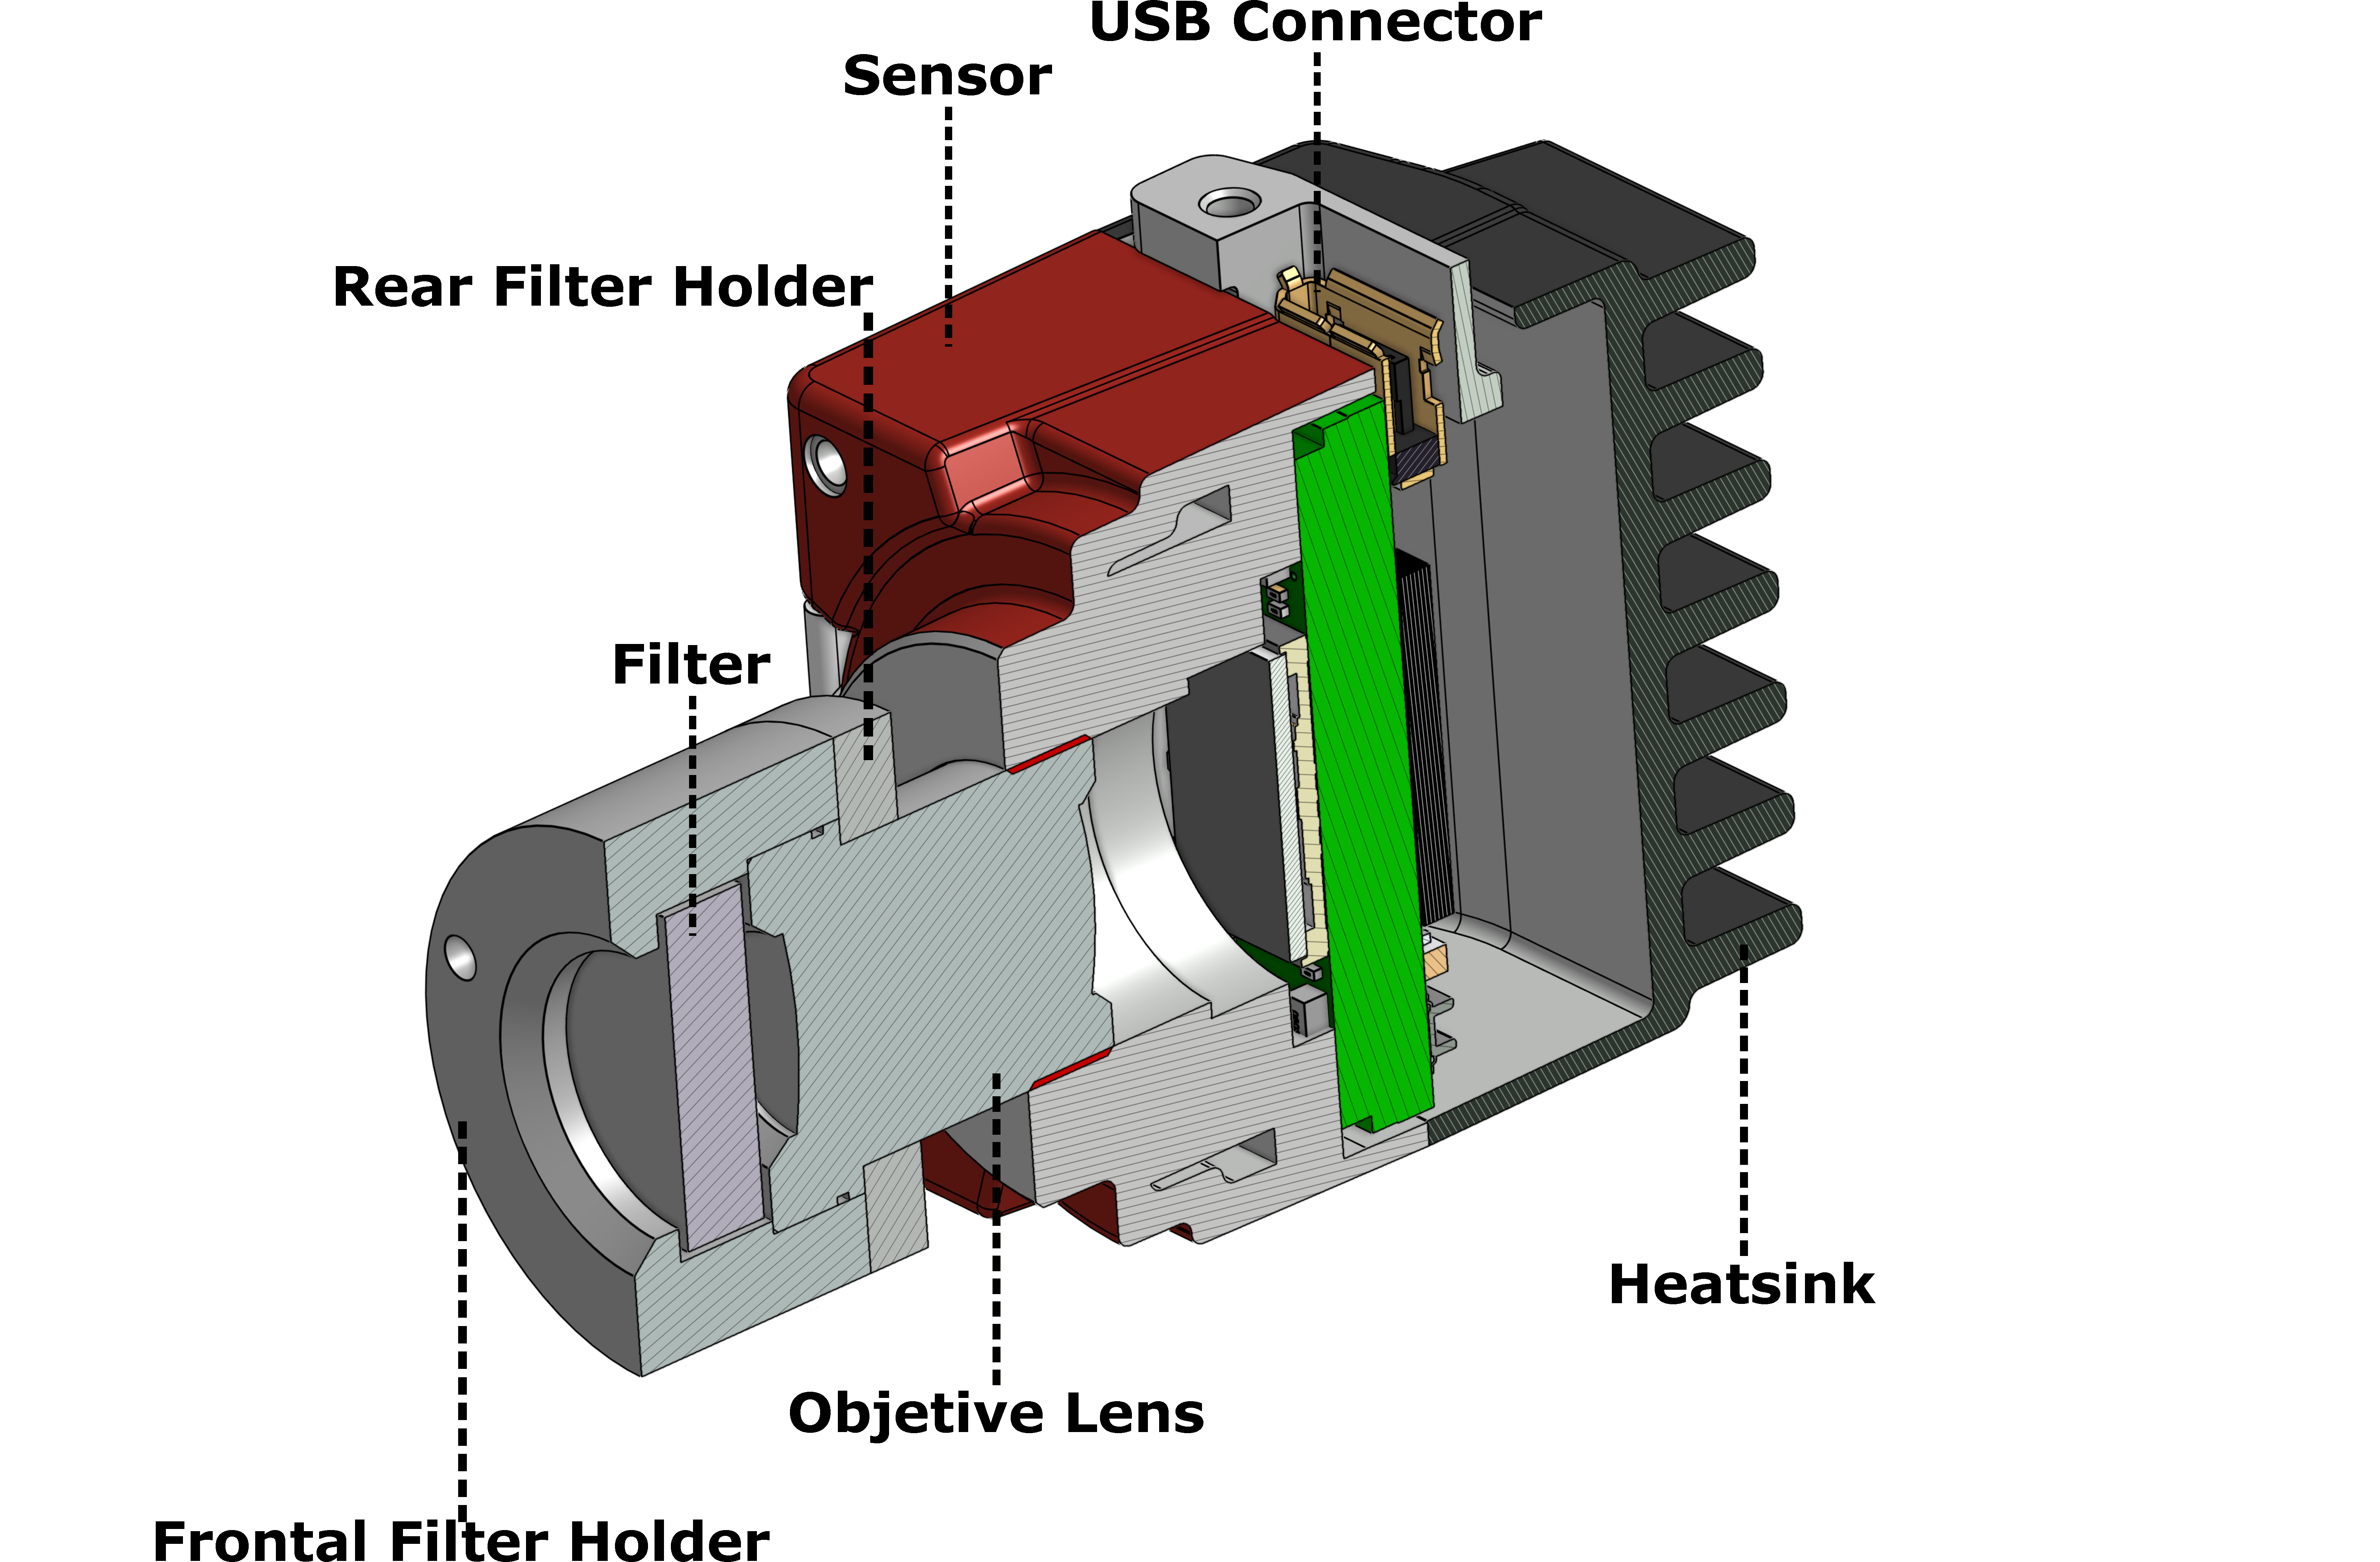
\includegraphics[width=\linewidth]{Figures/C4/NIR1.pdf}
            \caption{Sistema 6 (NIR): montaje del objetivo y filtro. El soporte evita desalineamientos y asegura la óptica en su eje.}
            \label{fig:lens_filter_mount_nir}
        \end{subfigure}
        \hfill
        \begin{subfigure}[b]{0.47\linewidth}
            \centering
            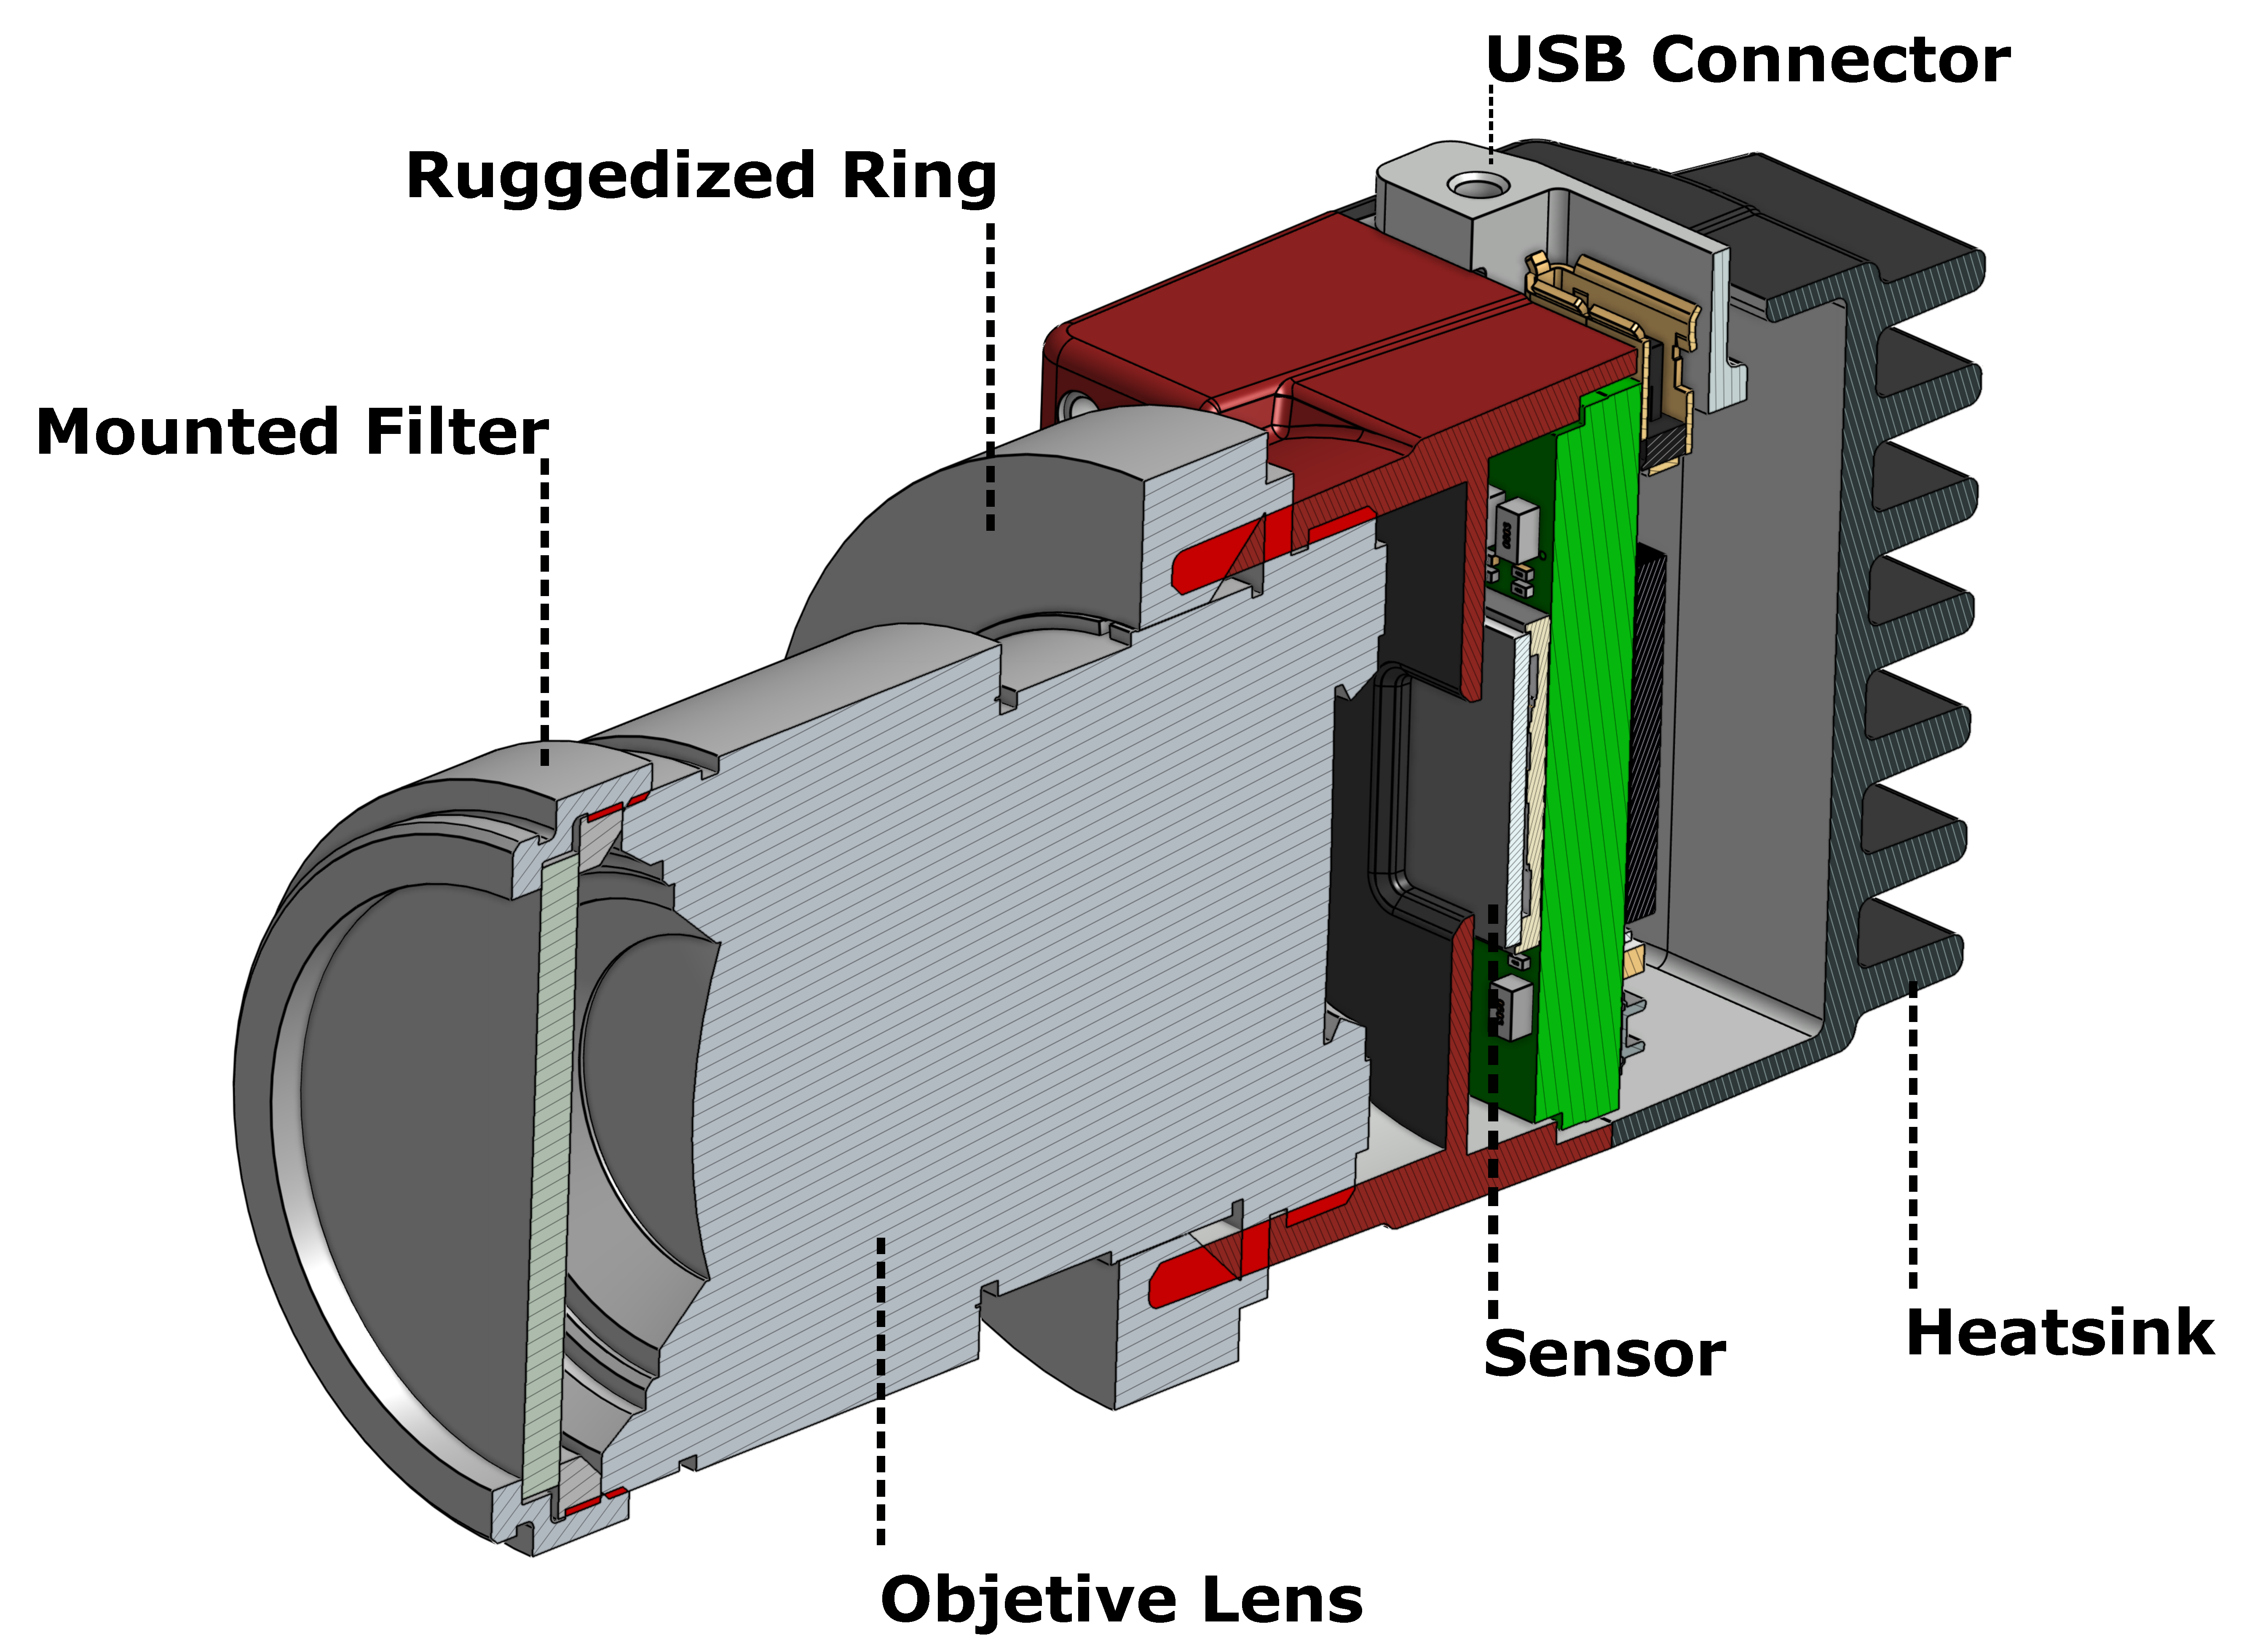
\includegraphics[width=\linewidth]{Figures/C4/VIS1.pdf}
            \caption{Sistema 7 (VIS): conector micro USB‑B para alimentación y datos.}
            \label{fig:micro_usb_vis}
        \end{subfigure}
        \caption{Componentes destacados de los sistemas ópticos seleccionados para el prototipo: NIR (izquierda) y VIS (derecha).}
        \label{fig:sistemas_opticos_componentes}
    \end{figure}


    
    

  % \subsection{Integración con la plataforma UAV}
  %   % → Describir interfaz mecánica, centro de masas, cableado
  %   %   y sistema de amortiguación de vibraciones.

  % \subsection{Validaciones funcionales de taller}
  %   % → Pruebas de alineamiento, sellado de luz parásita y peso final.
  %   %   Tabla de verificación contra los requisitos de la Sección 1.1.

\section{Pruebas de operación}
  \subsection{Script de control y adquisición}
    \label{sec:script_control_adquisicion}
    
    Con el propósito de automatizar el proceso de captura, procesamiento y almacenamiento de imágenes multiespectrales durante los vuelos o pruebas en banco, se desarrolló un script en lenguaje Python que permite la adquisición simultánea de imágenes en el espectro visible (VIS) y cercano al infrarrojo (NIR), integrando además datos de posicionamiento global (GPS) en tiempo real.
    
    \noindent Este script constituye una adaptación del código de ejemplo provisto por la biblioteca \texttt{vmbpy}, correspondiente al SDK de \textit{Allied Vision}, y fue modificado sustancialmente para incluir manejo multihilo, escritura condicional de video, superposición de información telemétrica, y control por teclado durante la ejecución.
    
    \subsection{Estructura general del script}
    
    El flujo lógico del código se presenta en la Figura~\ref{fig:diagrama_script}, donde se destacan tres etapas fundamentales: (i) la inicialización del entorno y detección de cámaras, (ii) la adquisición concurrente de tramas mediante hilos productores, y (iii) el procesamiento y visualización de las imágenes mediante un hilo consumidor.
    
    \begin{figure}[!h]
        \centering
        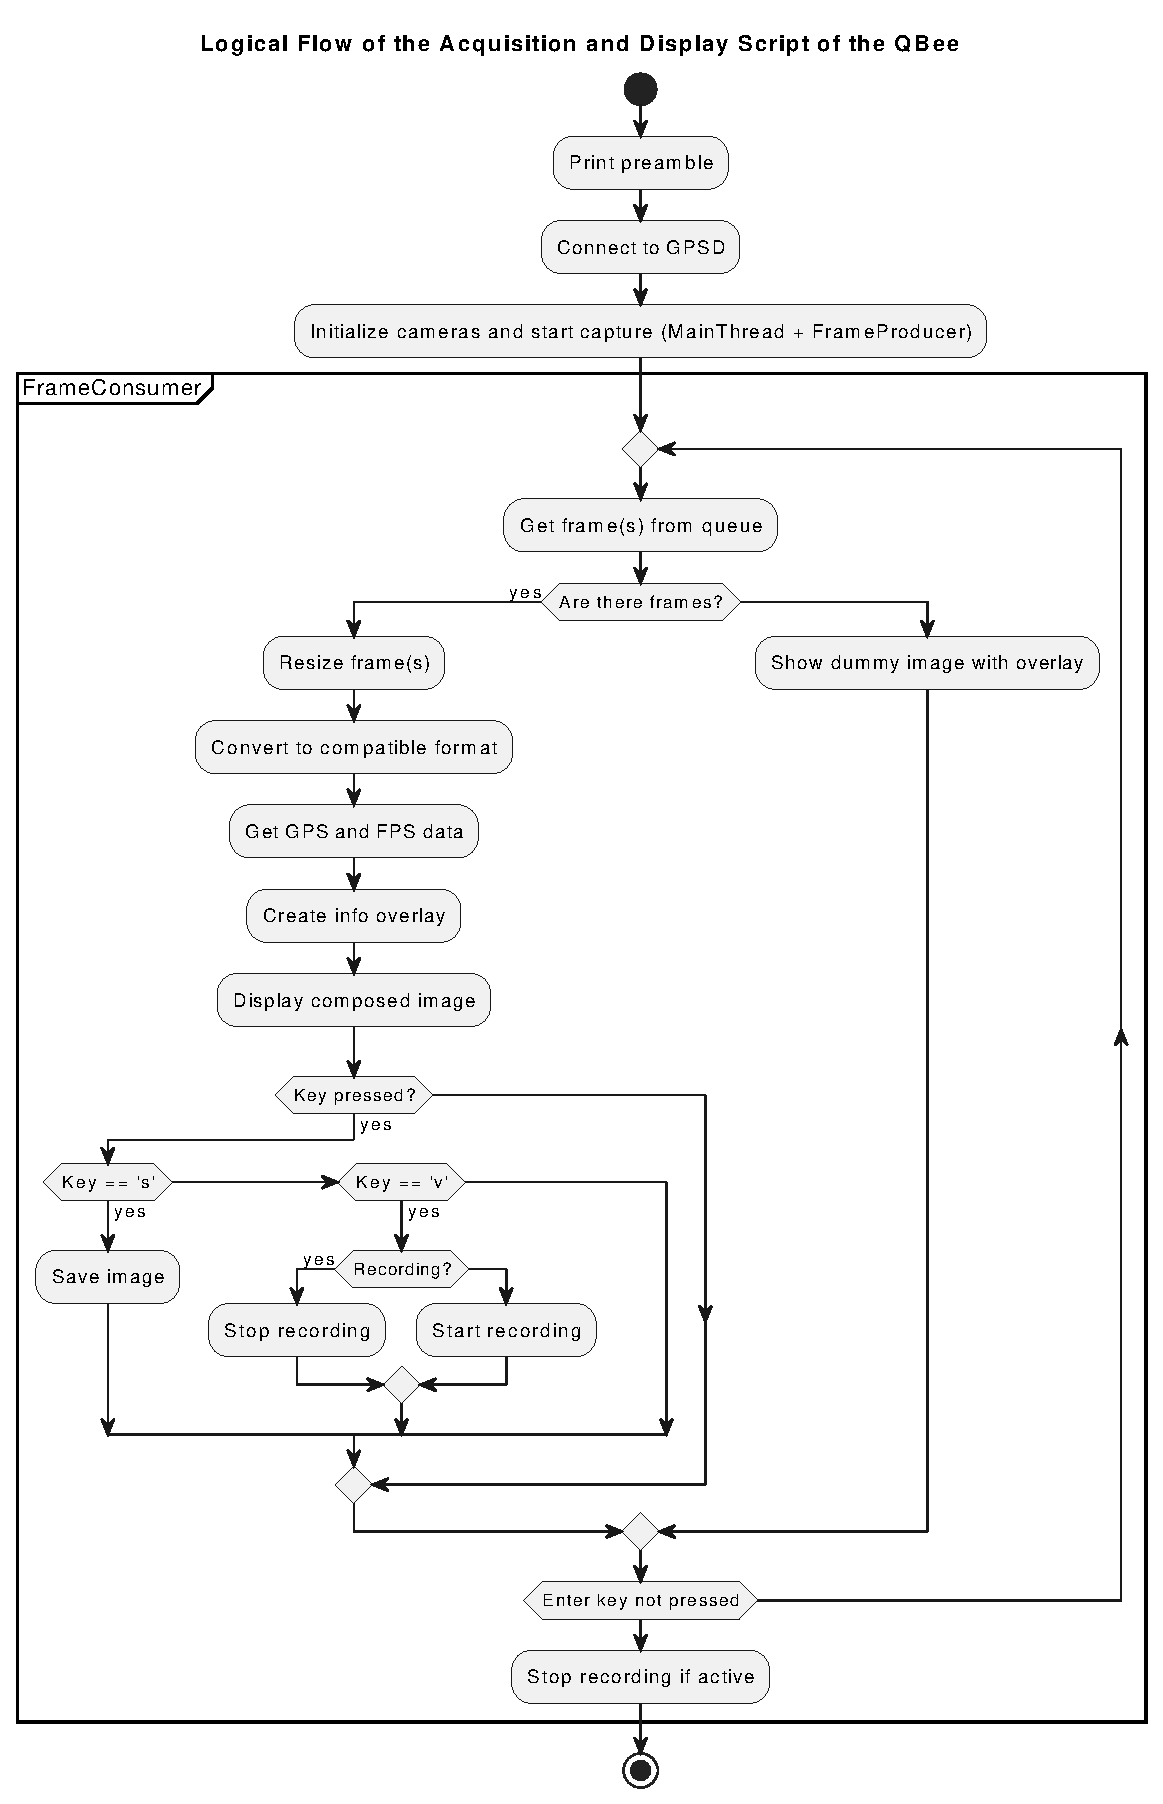
\includegraphics[trim = 0 0 0 1cm, clip, width=1\textwidth]{Figures/C4/OSU_main.pdf}
        \caption{Flujo lógico del script de adquisición y visualización de la QBee. Se integran múltiples cámaras, adquisición en paralelo y procesamiento en tiempo real.}
        \label{fig:diagrama_script}
    \end{figure}
    
    \subsection{Inicialización y adquisición}
    
    Durante la fase de inicialización, se establece una conexión con el servidor local de GPS (\texttt{gpsd}) utilizando la librería homónima. Paralelamente, se instancia la clase \texttt{MainThread}, responsable de detectar automáticamente todas las cámaras conectadas a través del sistema \texttt{VmbSystem}.\\
    
     Cada cámara detectada es asignada a un hilo independiente de la clase \texttt{FrameProducer}, la cual configura parámetros críticos como la resolución de adquisición, formato de pixel (\texttt{Mono8} o \texttt{Bgr8}), y el modo automático de exposición. Estos hilos se encargan de capturar tramas en tiempo real, estimar la tasa de cuadros por segundo (FPS) y encolar las imágenes en una estructura tipo FIFO (\texttt{queue.Queue}) para su posterior procesamiento.
    
    \subsection{Procesamiento, visualización y almacenamiento}
    
    La etapa central del sistema está contenida en la clase \texttt{FrameConsumer}, la cual opera como hilo consumidor. Esta clase realiza múltiples tareas en paralelo: (i) extrae tramas de la cola compartida, (ii) redimensiona las imágenes si la resolución de adquisición no coincide con la esperada (\SI[parse-numbers = false]{2592 \times 1944}{px}), (iii) convierte los formatos de imagen a RGB si es necesario, y (iv) concatena las imágenes capturadas por múltiples cámaras en un único mosaico horizontal.\\
    
    Sobre esta imagen compuesta se genera una barra de información (\textit{overlay}) que incluye los datos georreferenciados en tiempo real (latitud, longitud, altitud, velocidad, ángulo de rumbo y timestamp), además de la tasa de cuadros por segundo estimada para cada cámara. Esta superposición se construye como una matriz adicional que se apila verticalmente a la imagen original.\\
    
    El sistema también permite una interacción directa con el operador mediante teclas específicas:
    \begin{itemize}
        \item \textbf{\texttt{s}}: captura la imagen actual y la guarda en formato \texttt{JPEG}.
        \item \textbf{\texttt{v}}: inicia o detiene la grabación de video en formato \texttt{AVI}, con compresión \texttt{XVID}, a una frecuencia de 20 FPS.
        \item \textbf{\texttt{Enter}}: finaliza la ejecución del script y cierra todas las ventanas.
    \end{itemize}
    
    \subsection{Ejecución automática como servicio de sistema}
    
    Con el fin de garantizar un funcionamiento autónomo y minimizar la intervención del usuario, se diseñó un servicio de sistema en Linux (utilizando \texttt{systemd}) que permite la ejecución automática del script tan pronto como el dispositivo inicia. Este servicio fue instalado y habilitado en el sistema operativo de una Raspberry Pi 4 modelo B equipada con 8 GB de memoria RAM.
    
    Gracias a esta configuración, el sistema conocido como \texttt{QBee} se activa automáticamente al conectar la batería externa a la Raspberry Pi, sin requerir intervención adicional ni acceso al entorno gráfico. Inmediatamente después del arranque, el script inicia la captura de imágenes y comienza a almacenarlas en la memoria interna, lo que resulta particularmente útil para operaciones en campo, donde no es viable iniciar el sistema manualmente.
    
    \subsection{Robustez y tolerancia a fallos}
    
    Durante la ejecución, el sistema cuenta con mecanismos de tolerancia a errores. Por ejemplo, si el buffer de imágenes se encuentra lleno, los hilos productores omiten la encolación de nuevas tramas para evitar bloqueos. Asimismo, si no se detecta ninguna cámara activa, se genera una imagen dummy con un mensaje de advertencia.\\
    
    Las tramas obtenidas se almacenan temporalmente en memoria, lo que permite minimizar la latencia entre adquisición y visualización. La sincronización entre hilos se realiza mediante eventos y bloqueos controlados, garantizando la integridad de los datos entre productores y consumidores.
    
    \subsection{Dependencias y entorno de ejecución}
    
    El script fue ejecutado sobre el sistema operativo Raspberry Pi OS (basado en Debian) en una Raspberry Pi 4 modelo B. Se utilizó Python 3.8 y las siguientes dependencias: \texttt{vmbpy}, \texttt{opencv-python}, \texttt{gpsd-py3}, \texttt{numpy}, \texttt{threading}, \texttt{queue} y \texttt{keyboard}. La visualización se realizó mediante la salida HDMI de la Raspberry, y se requirió establecer la variable de entorno \texttt{DISPLAY=":0"} para habilitar la salida gráfica de OpenCV.

    \subsection{Control remoto del dispositivo \texttt{QBee}}

    Además de su capacidad de operación autónoma en campo, el sistema \texttt{QBee} fue diseñado con funcionalidad de control remoto, permitiendo su supervisión y operación desde dispositivos externos como computadores personales, tabletas o teléfonos móviles. Esta característica extiende significativamente la versatilidad del sistema, facilitando tanto pruebas en laboratorio como operaciones a distancia en entornos de difícil acceso.\\
    
    Existen dos métodos principales para acceder de forma remota a la interfaz gráfica del sistema:
    
    \paragraph{1. Conexión local mediante VNC}
    
    El primer método consiste en conectarse directamente a la Raspberry Pi 4 que ejecuta el sistema \texttt{QBee} mediante el protocolo VNC (\textit{Virtual Network Computing}). Para ello, es necesario que la Raspberry esté conectada a una red Wi-Fi previamente configurada para su conexión automática. Asimismo, el dispositivo de control (computador o móvil) debe encontrarse dentro de la misma red local.\\
    
    Una vez cumplida esta condición, el usuario puede acceder a la interfaz gráfica de la Raspberry Pi introduciendo su dirección IP o una dirección local estática configurada mediante el sistema operativo Raspberry Pi OS. Para completar el acceso, se requiere conocer las credenciales de autenticación (nombre de usuario y contraseña) establecidas previamente en el sistema.
    
    \paragraph{2. Acceso global mediante Raspberry Pi Connect}
    
    El segundo método se basa en el uso de \textit{Raspberry Pi Connect}, un servicio gratuito proporcionado por la fundación Raspberry Pi. Este permite acceder a la interfaz gráfica del sistema desde cualquier lugar con conexión a Internet, sin necesidad de estar dentro de la misma red local.\\
    
    Para habilitar esta funcionalidad, la Raspberry Pi debe estar vinculada a una cuenta en el servicio \textit{Raspberry Pi Connect} y tener acceso a Internet mediante una red Wi-Fi registrada previamente. Una vez registrado el dispositivo, el usuario puede iniciar sesión en el portal de Raspberry Pi y conectarse directamente a su interfaz gráfica a través del navegador.  \\
    
    
    En ambos métodos, el usuario obtiene acceso completo al entorno de escritorio de la Raspberry Pi. Como se ha descrito en las secciones anteriores, el script de adquisición de \texttt{QBee} se ejecuta automáticamente al iniciar el sistema, lo que da lugar a la apertura de una ventana de visualización en tiempo real de las imágenes capturadas.\\
    
    Desde esta interfaz remota, el usuario puede interactuar directamente con el sistema utilizando un teclado virtual o físico para ejecutar acciones de control. Entre las funcionalidades disponibles se encuentran:
    \begin{itemize}
        \item Presionar la tecla \texttt{s} para capturar y guardar una imagen.
        \item Presionar la tecla \texttt{v} para iniciar o detener la grabación de video.
        \item Presionar la tecla \texttt{Enter} para finalizar la ejecución del script.
    \end{itemize}
    
    Esta capacidad de control remoto permite verificar el correcto funcionamiento del sistema en tiempo real, supervisar condiciones de operación, y capturar eventos relevantes sin necesidad de intervención física directa sobre el dispositivo.\\
    
    
    Adicionalmente, el sistema \texttt{QBee} fue configurado para permitir actualizaciones remotas del código fuente del script mediante el sistema de control de versiones \texttt{Git}. El script está vinculado a un repositorio privado alojado en la plataforma \texttt{GitHub}, lo que permite a los usuarios autenticados realizar \textit{pull} de actualizaciones desde cualquier ubicación con acceso remoto al dispositivo. Esta funcionalidad permite una mejora continua del sistema, facilitando la depuración, implementación de nuevas funcionalidades y adaptaciones específicas sin necesidad de acceso físico al hardware.
    
    
    
    

  \subsection{Escenarios de prueba}
    Los escenarios de prueba definidos para validar el correcto funcionamiento del sistema \textit{QBee} se clasifican en dos grupos principales: (i) pruebas terrestres en condiciones controladas, y (ii) pruebas en vuelo.

    \subsubsection{Pruebas terrestres}
    
        Antes de cualquier despliegue aéreo, es indispensable realizar pruebas en tierra que permitan validar el sistema en condiciones controladas, sin desplazamiento y sin exposición a ambientes extremos. En este contexto, se define como ambiente extremo cualquier entorno cuya temperatura supere los valores comunes encontrados en las principales ciudades colombianas (\SI{\leq 40}{\celsius}), o que implique lluvia, alta humedad o condiciones de iluminación nocturna.
        
        \noindent Dado que el sistema \textit{QBee} no cuenta con una fuente de iluminación activa, las pruebas se realizan exclusivamente durante el día, aprovechando la luz solar como fuente principal para la adquisición de imágenes multiespectrales.
        
        \noindent El objetivo de estas pruebas es verificar el comportamiento general del sistema en condiciones operativas normales. En particular, se evalúa:
        
        \begin{itemize}
        \item La correcta inicialización automática del script de adquisición al encender el dispositivo.
        \item La funcionalidad de captura de imágenes al presionar la tecla \texttt{s}.
        \item La grabación de video y su detención mediante la tecla \texttt{v}.
        \item La estabilidad del dispositivo al operar durante largos periodos de tiempo.
        \end{itemize}
        
        \noindent Las pruebas se realizaron utilizando dos formas de alimentación:
        \begin{itemize}
        \item \textbf{Fuente directa:} mediante un adaptador USB-C conectado a una toma de corriente convencional.
        \item \textbf{Fuente interna:} a partir de la bater'ia recargable integrada en la carcasa del \textit{QBee}.
        \end{itemize}
        
        \noindent Una de las pruebas más relevantes consisti'o en la captura de una imagen utilizando la tecla \texttt{s}, ya fuera desde un teclado conectado directamente a la Raspberry Pi 4 o mediante acceso remoto. En la Figura~\ref{fig:captura_prueba_remota} se presenta un ejemplo de imagen capturada en estas condiciones, utilizando un tel'efono inteligente para el control remoto del sistema. La prueba confirma el correcto funcionamiento de ambos canales (VIS y NIR), evidenciando que la captura simult'anea se realiza de manera sincronizada, y que el sistema responde adecuadamente a la orden de captura en tiempo real.
        
        \begin{figure}[h]
        \centering
        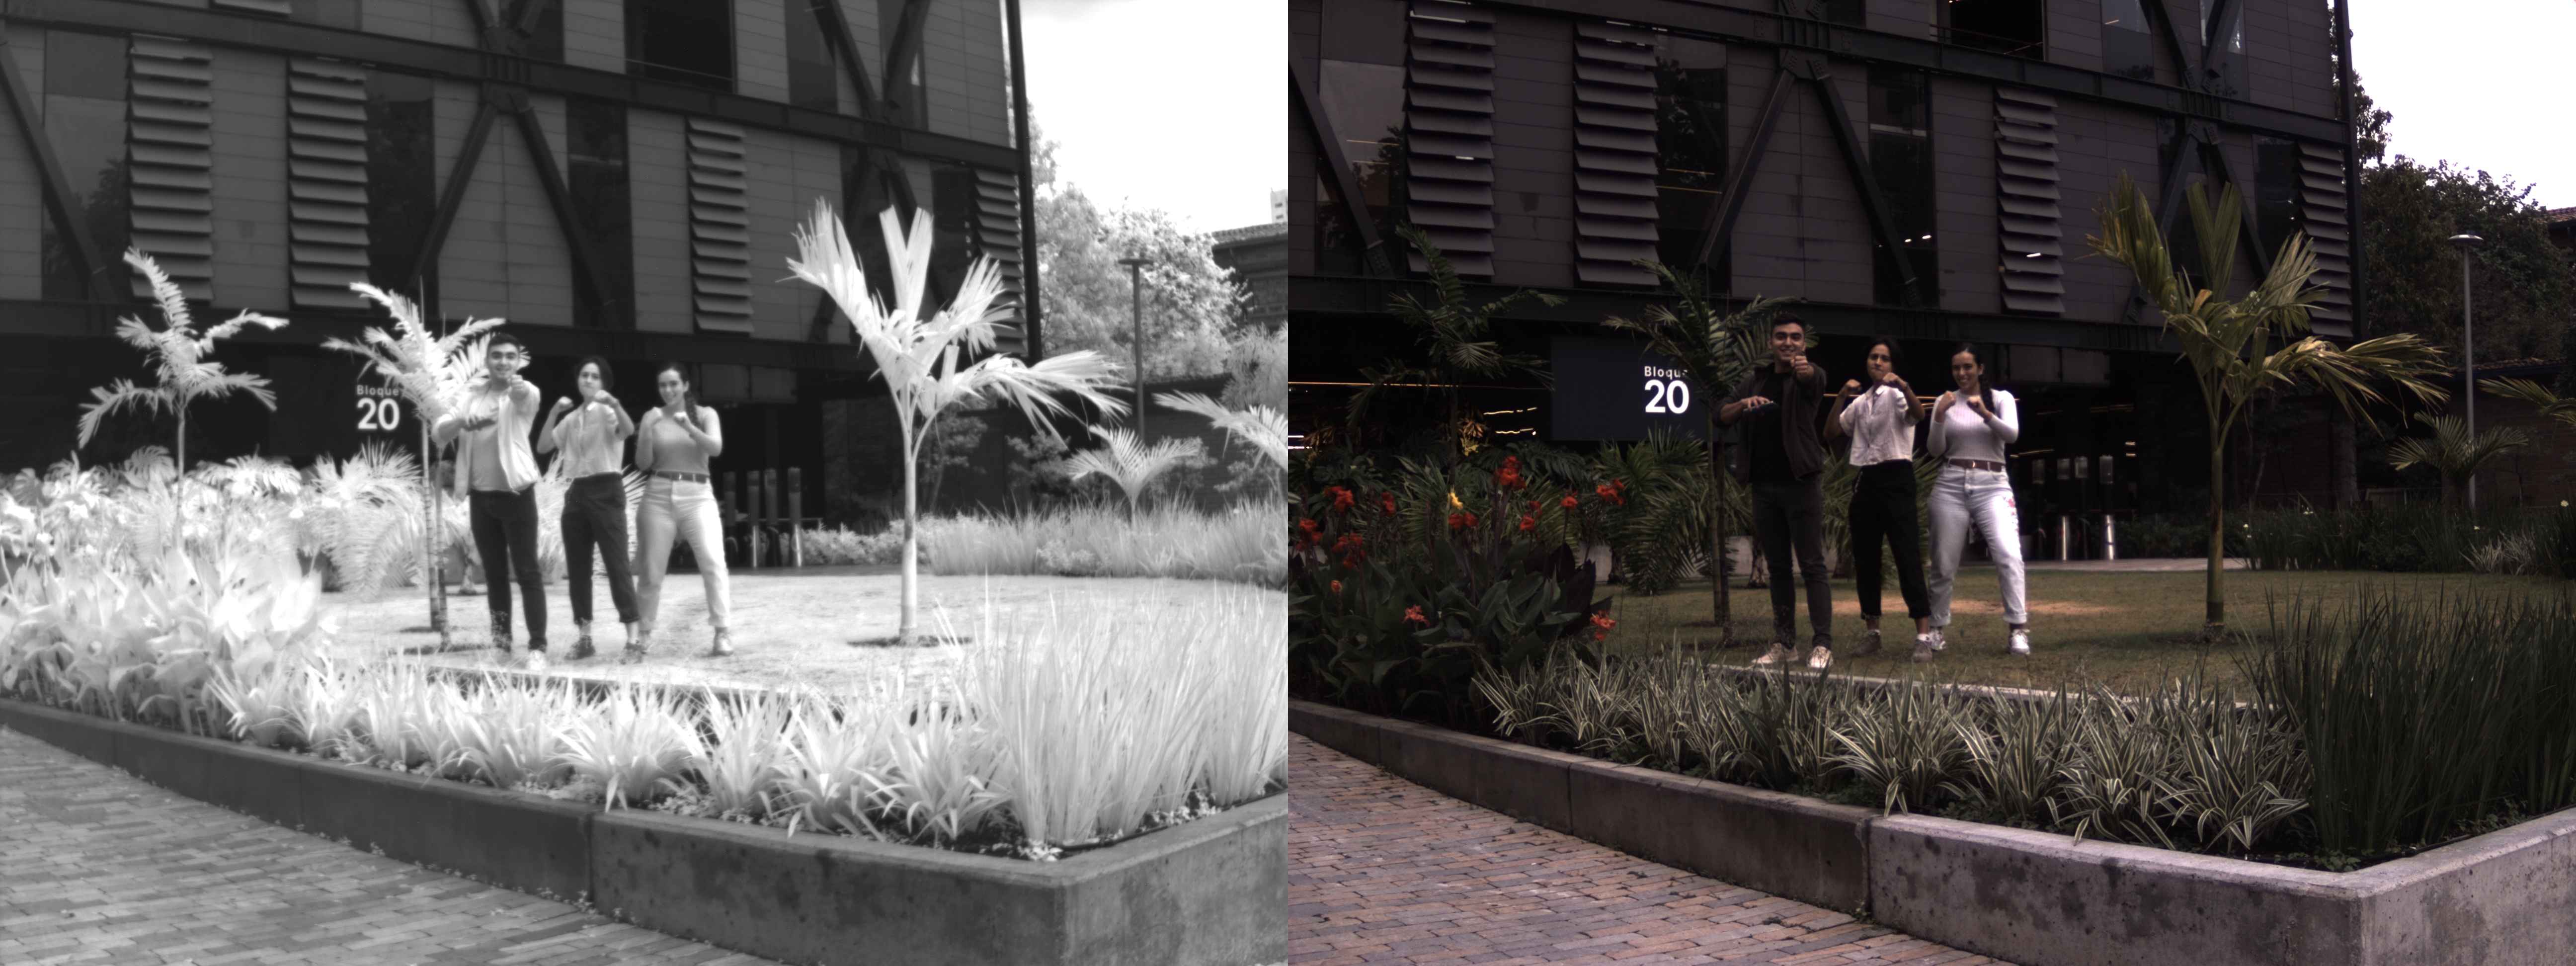
\includegraphics[width=1\textwidth]{Figures/C4/captured_image_20240201_174102.jpg}
        \caption{Captura de imagen realizada durante prueba terrestre mediante control remoto desde un tel'efono inteligente. La imagen muestra la composici'on de ambos canales VIS y NIR, confirmando la funcionalidad del sistema \textit{QBee} en condiciones operativas reales.}
        \label{fig:captura_prueba_remota}
        \end{figure}
        
        \noindent En complemento, en la Figura~\ref{fig:gps_overlay_visual} se presenta un ejemplo de visualización del sistema de coordenadas geográficas en tiempo real. En la parte superior de la imagen se observa la superposición del texto con la latitud, longitud, altitud, velocidad y rumbo extraídos del módulo GPS integrado en la \textit{QBee}. Esta funcionalidad es crítica para asegurar la trazabilidad espacial de las imágenes adquiridas y para su posterior georreferenciación.

        \begin{figure}[h]
            \centering
            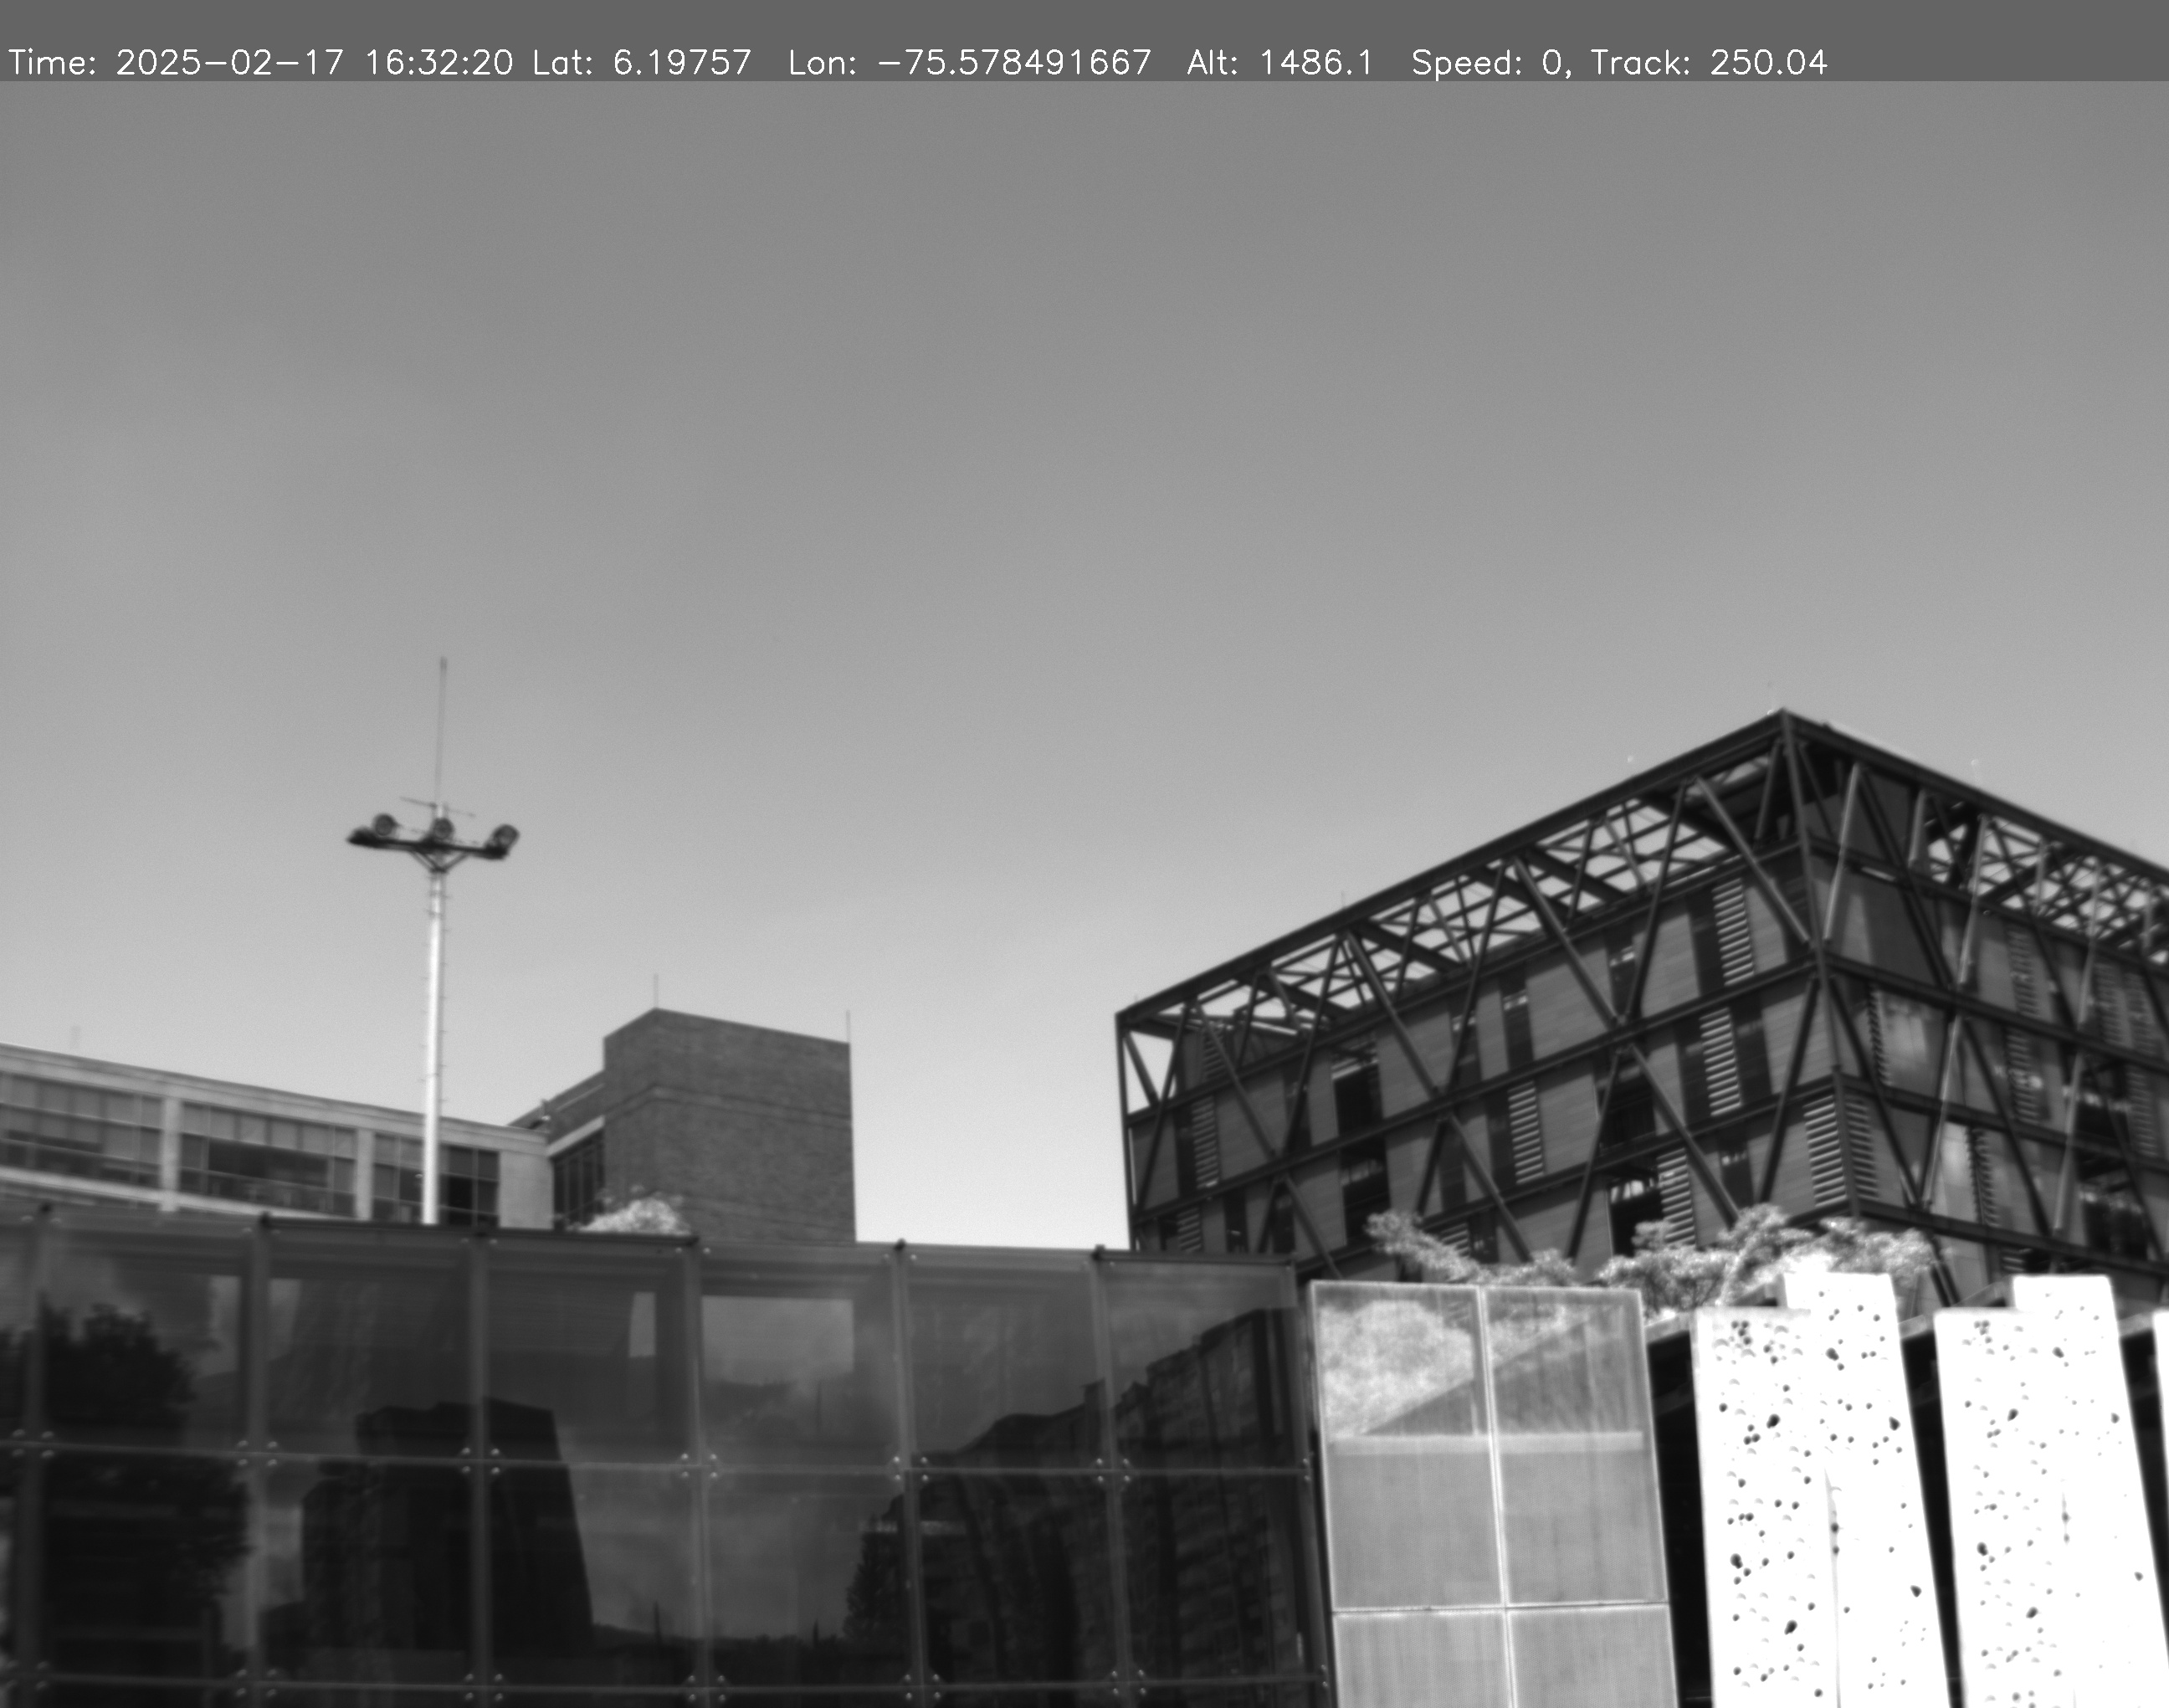
\includegraphics[width=0.9\textwidth]{Figures/C4/captured_image_20250217_113221.jpg}
            \caption{Visualización del sistema de coordenadas geográficas (GPS) en tiempo real sobre la imagen capturada. Se muestran latitud, longitud, altitud, velocidad y rumbo, extraídos automáticamente del módulo GPS durante las pruebas.}
            \label{fig:gps_overlay_visual}
        \end{figure}



    \subsubsection{Pruebas en superficie en condiciones extremas}

    Durante la VII Campa~na A'erea y XI Expedici'on Cient'ifica a la Ant'artida organizada por la Fuerza A'erea Colombiana, el sistema \textit{QBee} fue sometido a una prueba de funcionamiento en condiciones clim'aticas extremas. En este escenario, se enfrent'o a temperaturas diurnas promedio cercanas a los \SI{0}{\celsius}, significativamente inferiores a las condiciones habituales en las cuales opera el sistema.
    
    \noindent El objetivo principal de esta prueba fue evaluar la capacidad del dispositivo para operar de manera confiable en ambientes fr'ios. Se identific'o que, bajo estas condiciones, el sistema present'o fallas intermitentes en su funcionamiento: en algunas ocasiones la \textit{QBee} no inici'o correctamente, o no fue capaz de realizar la grabaci'on de video como lo hace regularmente. Estas fallas pueden estar asociadas a una inicializaci'on deficiente del sistema de procesamiento (Raspberry Pi 4), o a alteraciones en el comportamiento de los sensores VIS y NIR debido a la baja temperatura.
    
    \noindent No obstante, tambi'en se registraron casos exitosos de captura de video, lo cual demuestra que el sistema \textit{QBee} puede llegar a operar de forma funcional en condiciones de fr'io extremo. Estos resultados parciales abren la posibilidad de implementar ajustes de hardware y software para robustecer el funcionamiento del sistema en ambientes m'as hostiles. Queda como trabajo futuro el estudio detallado de las causas espec'ificas de las fallas observadas, as'i como la exploraci'on de soluciones que permitan una operaci'on m'as confiable en entornos como la Ant'artida.
    
    \noindent A pesar de los resultados mixtos, se concluye que el sistema actual no est'a dise~nado para misiones operativas regulares en la Ant'artida u otras regiones con condiciones ambientales similares, sin modificaciones adicionales en aislamiento t'ermico, tolerancia de componentes y procedimientos de inicializaci'on.
    
    \begin{figure}[h]
    \centering
    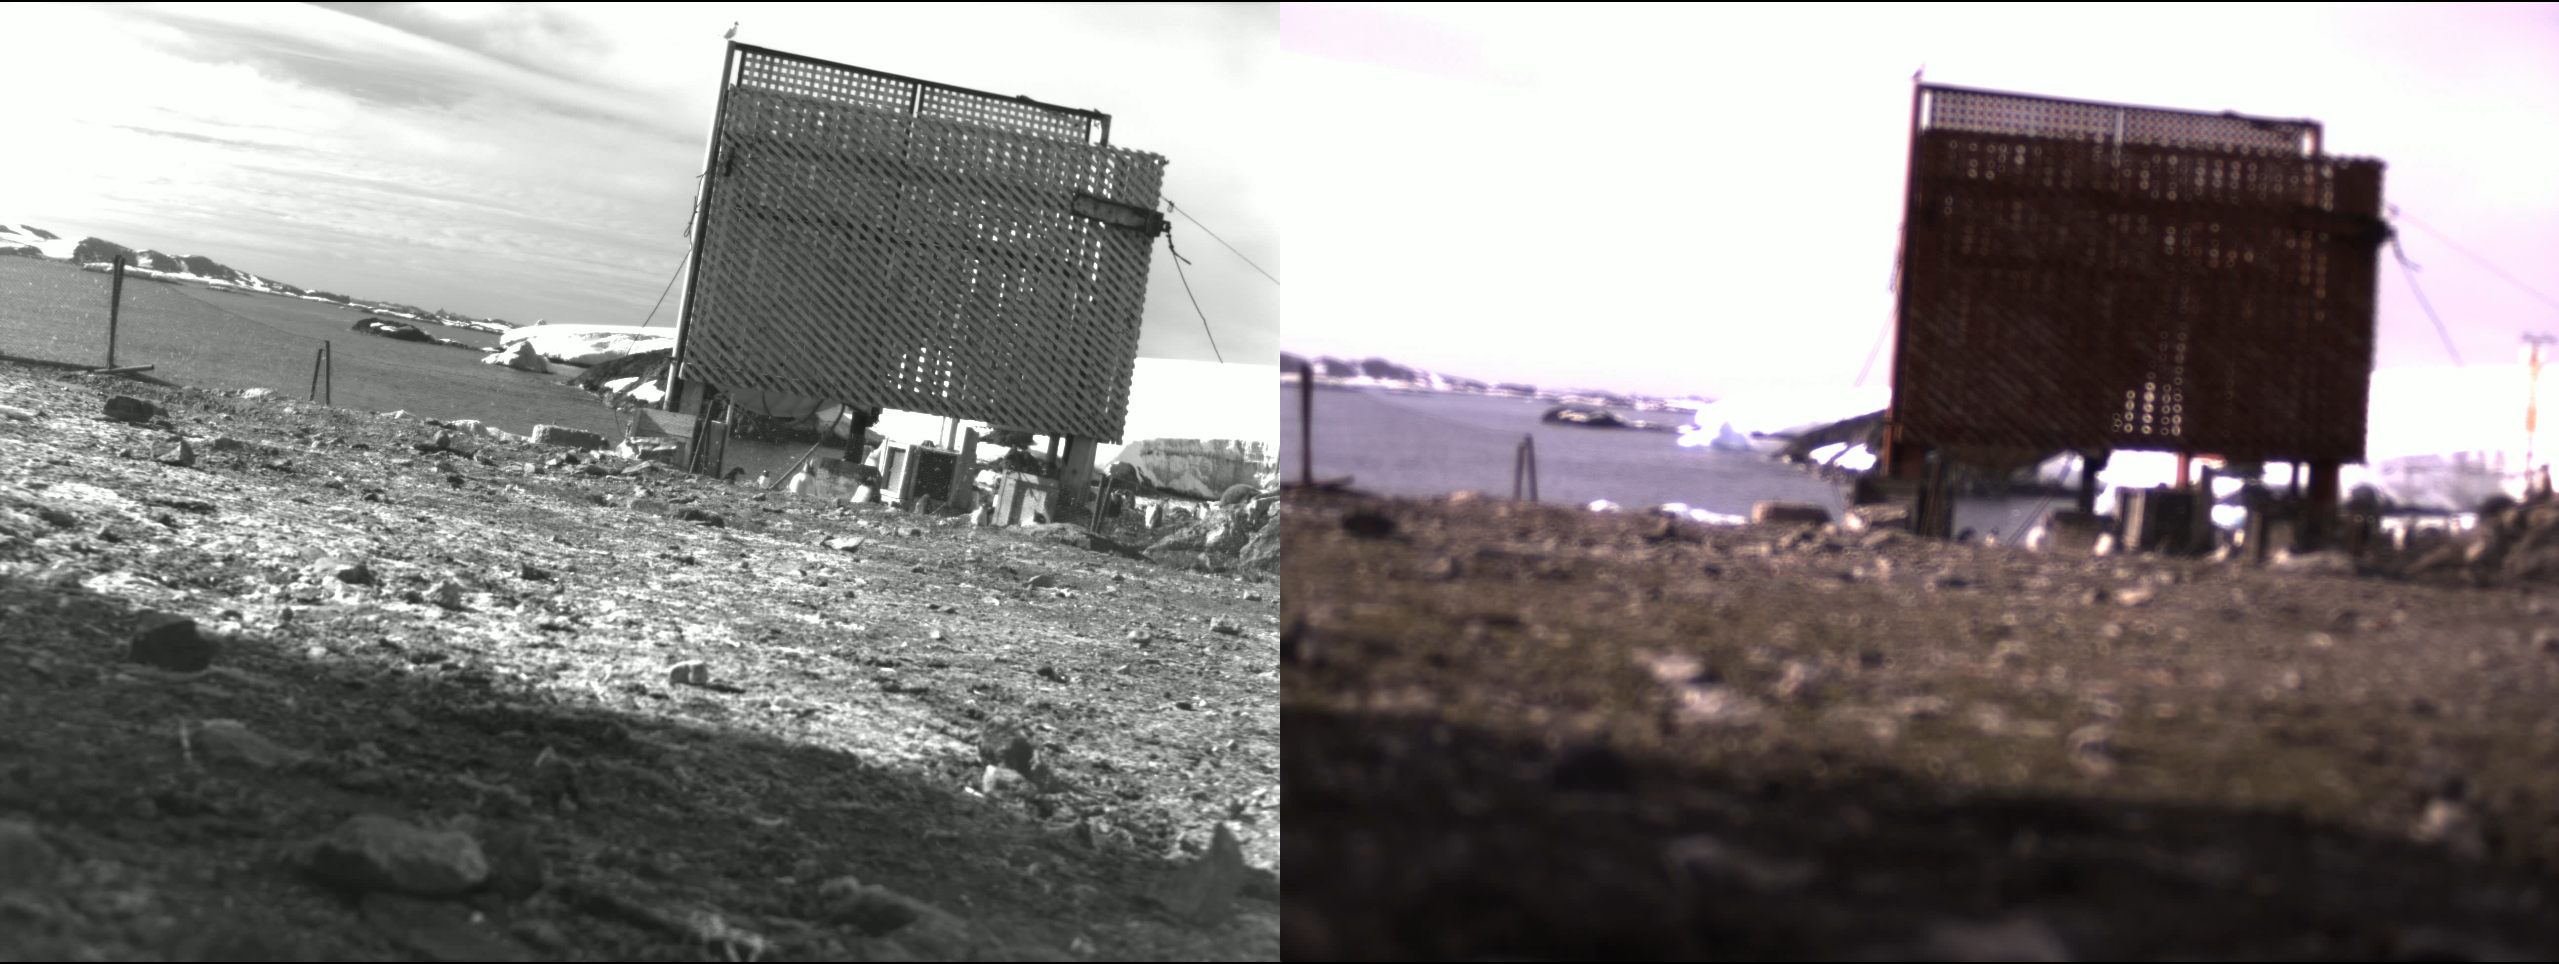
\includegraphics[width=1\textwidth]{Figures/C4/pinguinos.png}
    \caption{Captura de video realizada exitosamente durante la expedición científica en la Antártida. La imagen confirma que, a pesar de las condiciones extremas, el sistema \textit{QBee} En la imagen se aprecia que la cámara visible no se encuentra correctamente enfocada, lo que puede deberse a un mal ajuste de la distancia entre el objetivo y el sensor. Sin embargo, este tipo de desajuste es corregible mediante ajuste mecánico y no afecta el funcionamiento general del sistema \textit{QBee}. fue capaz de operar y registrar datos multiespectrales de forma puntual.}
    \label{fig:prueba_antartida}
    \end{figure}

    \subsubsection{Pruebas en vuelo}

    Las pruebas en vuelo del sistema \textit{QBee} fueron posibles gracias a la colaboraci'on con la Fuerza A'erea Colombiana, la cual facilit'o el montaje del dispositivo en distintas aeronaves de su flota. En una primera prueba, la unidad \textit{QBee} fue instalada a bordo de una aeronave Cessna 208 Caravan, realizando un vuelo a una altitud aproximada de 5000 pies.
    
    \noindent El vuelo se desarroll'o en condiciones ideales, con un rumbo y comportamiento t'ipico de una ruta comercial y sin presencia de perturbaciones atmosf'ericas significativas. Durante toda la duraci'on del trayecto, el sistema oper'o de forma estable y sin presentar inconvenientes.
    
    \noindent Como parte de esta prueba, se verific'o la capacidad de monitoreo remoto del sistema utilizando una red Wi-Fi habilitada dentro de la aeronave, mediante la cual se accedi'o al entorno gr'afico de la Raspberry Pi utilizando el protocolo VNC. Esta conexi'on permiti'o observar en tiempo real la adquisici'on de datos por parte del sistema, confirmando la funcionalidad completa del script y la respuesta de los sensores.
    
    \begin{figure}[!h]
    \centering
    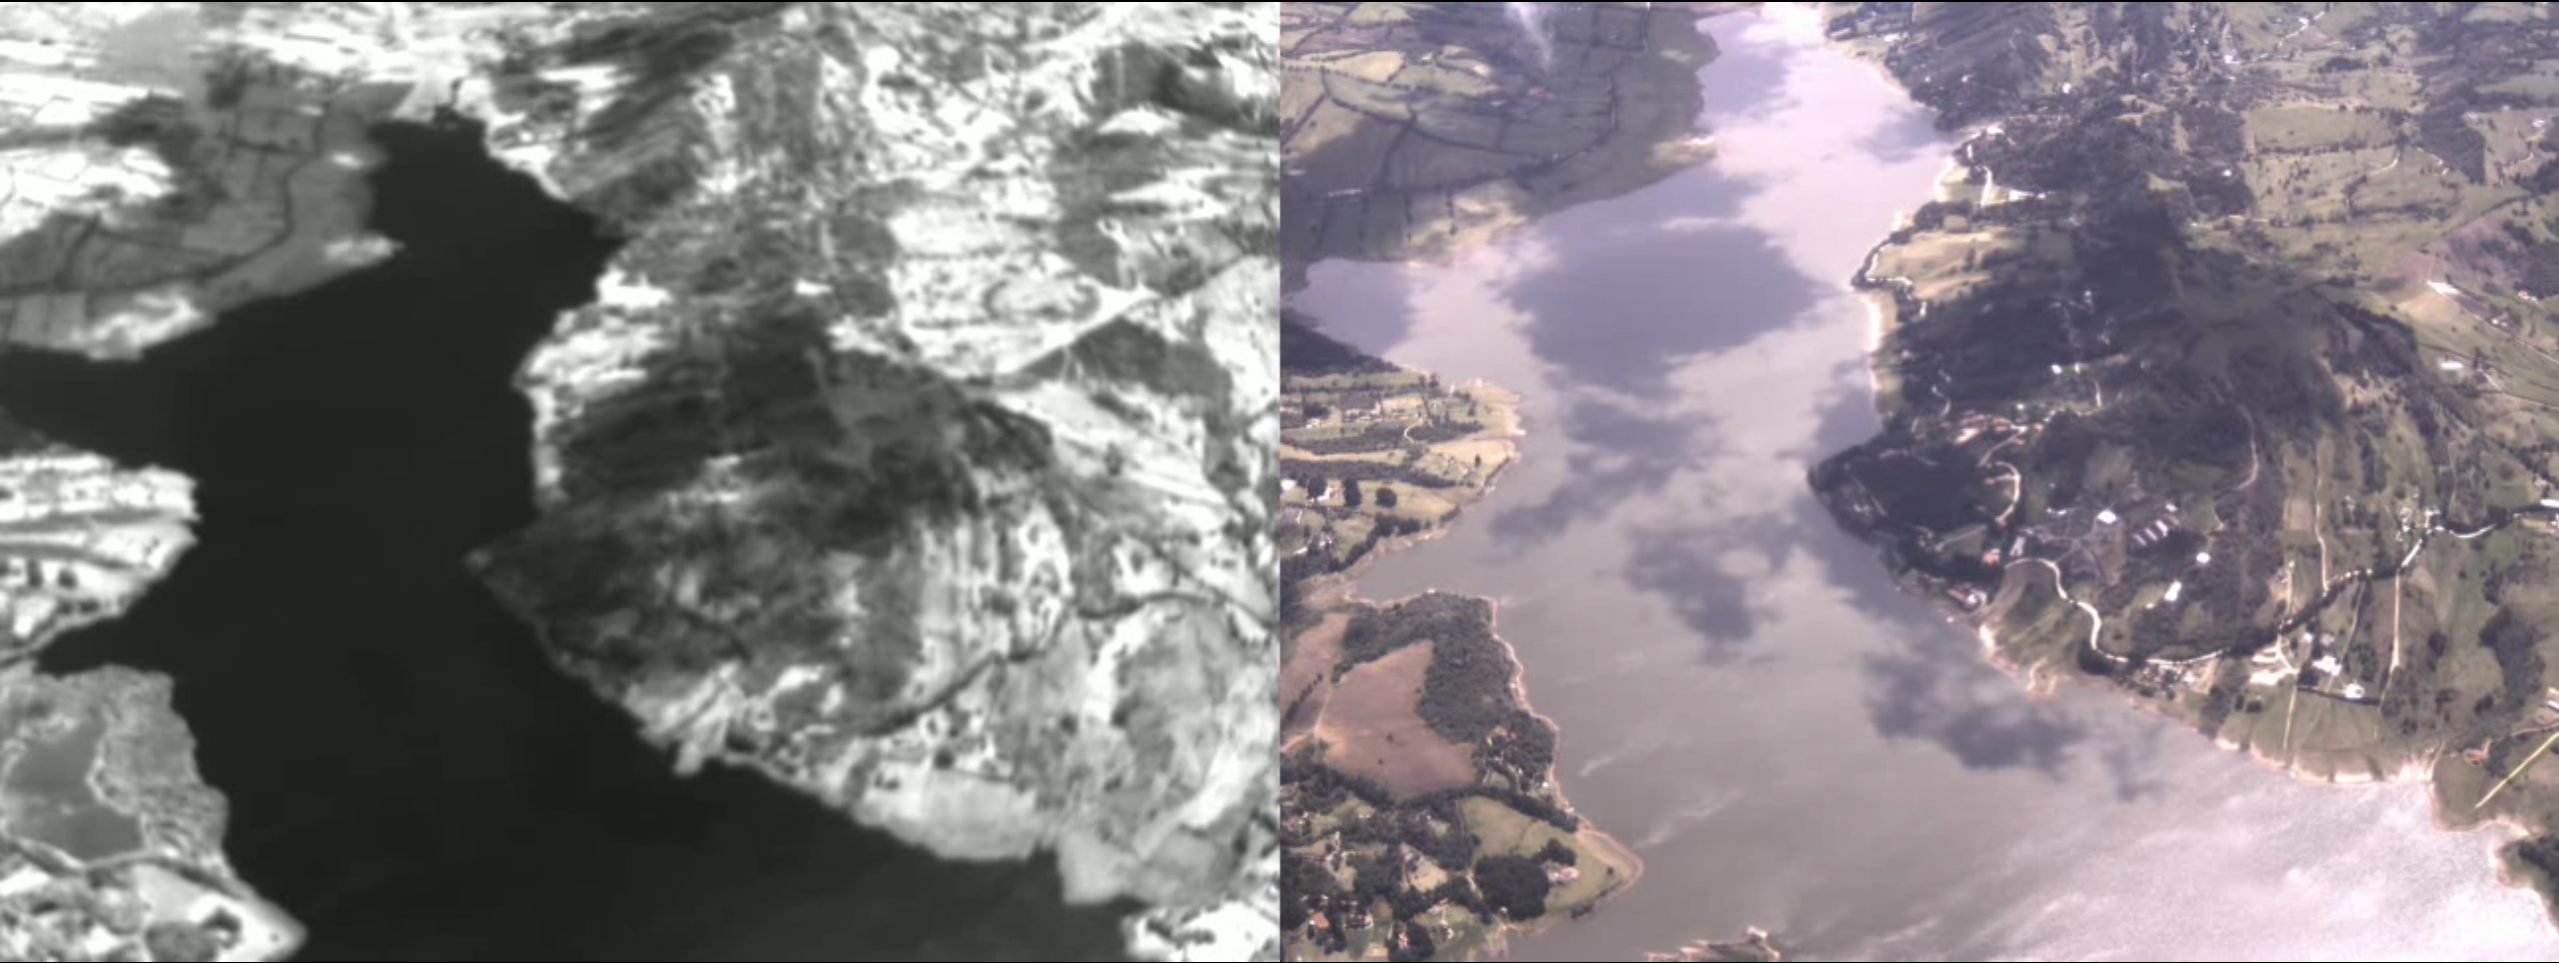
\includegraphics[width=1\textwidth]{Figures/C4/vuelo_caravan.png}
    \caption{Captura tomada durante el vuelo de prueba en la aeronave Cessna 208 Caravan. Se observ'o un comportamiento estable del sistema y transmisi'on remota exitosa mediante protocolo VNC.}
    \label{fig:prueba_vuelo}
    \end{figure}

    \noindent En una segunda prueba, la unidad \textit{QBee} fue montada a bordo de una aeronave de combate Tucano T-27, con el fin de validar su desempeño bajo condiciones de vuelo más exigentes. En este caso, no se contó con un sistema de monitoreo en tiempo real debido a las restricciones propias de la aeronave. Sin embargo, el sistema operó de forma autónoma durante la misión, registrando exitosamente la captura de video.

    \noindent A diferencia del vuelo en la Cessna Caravan, esta prueba presentó una complejidad adicional, ya que durante la operación se ejecutaron maniobras que alcanzaron aceleraciones de hasta 4g. A pesar de estas condiciones dinámicas, la \textit{QBee} logró completar su función de adquisición sin incidentes, lo cual representa un resultado relevante sobre la robustez mecánica y operativa del sistema.
    
    \begin{figure}[!h]
    \centering
    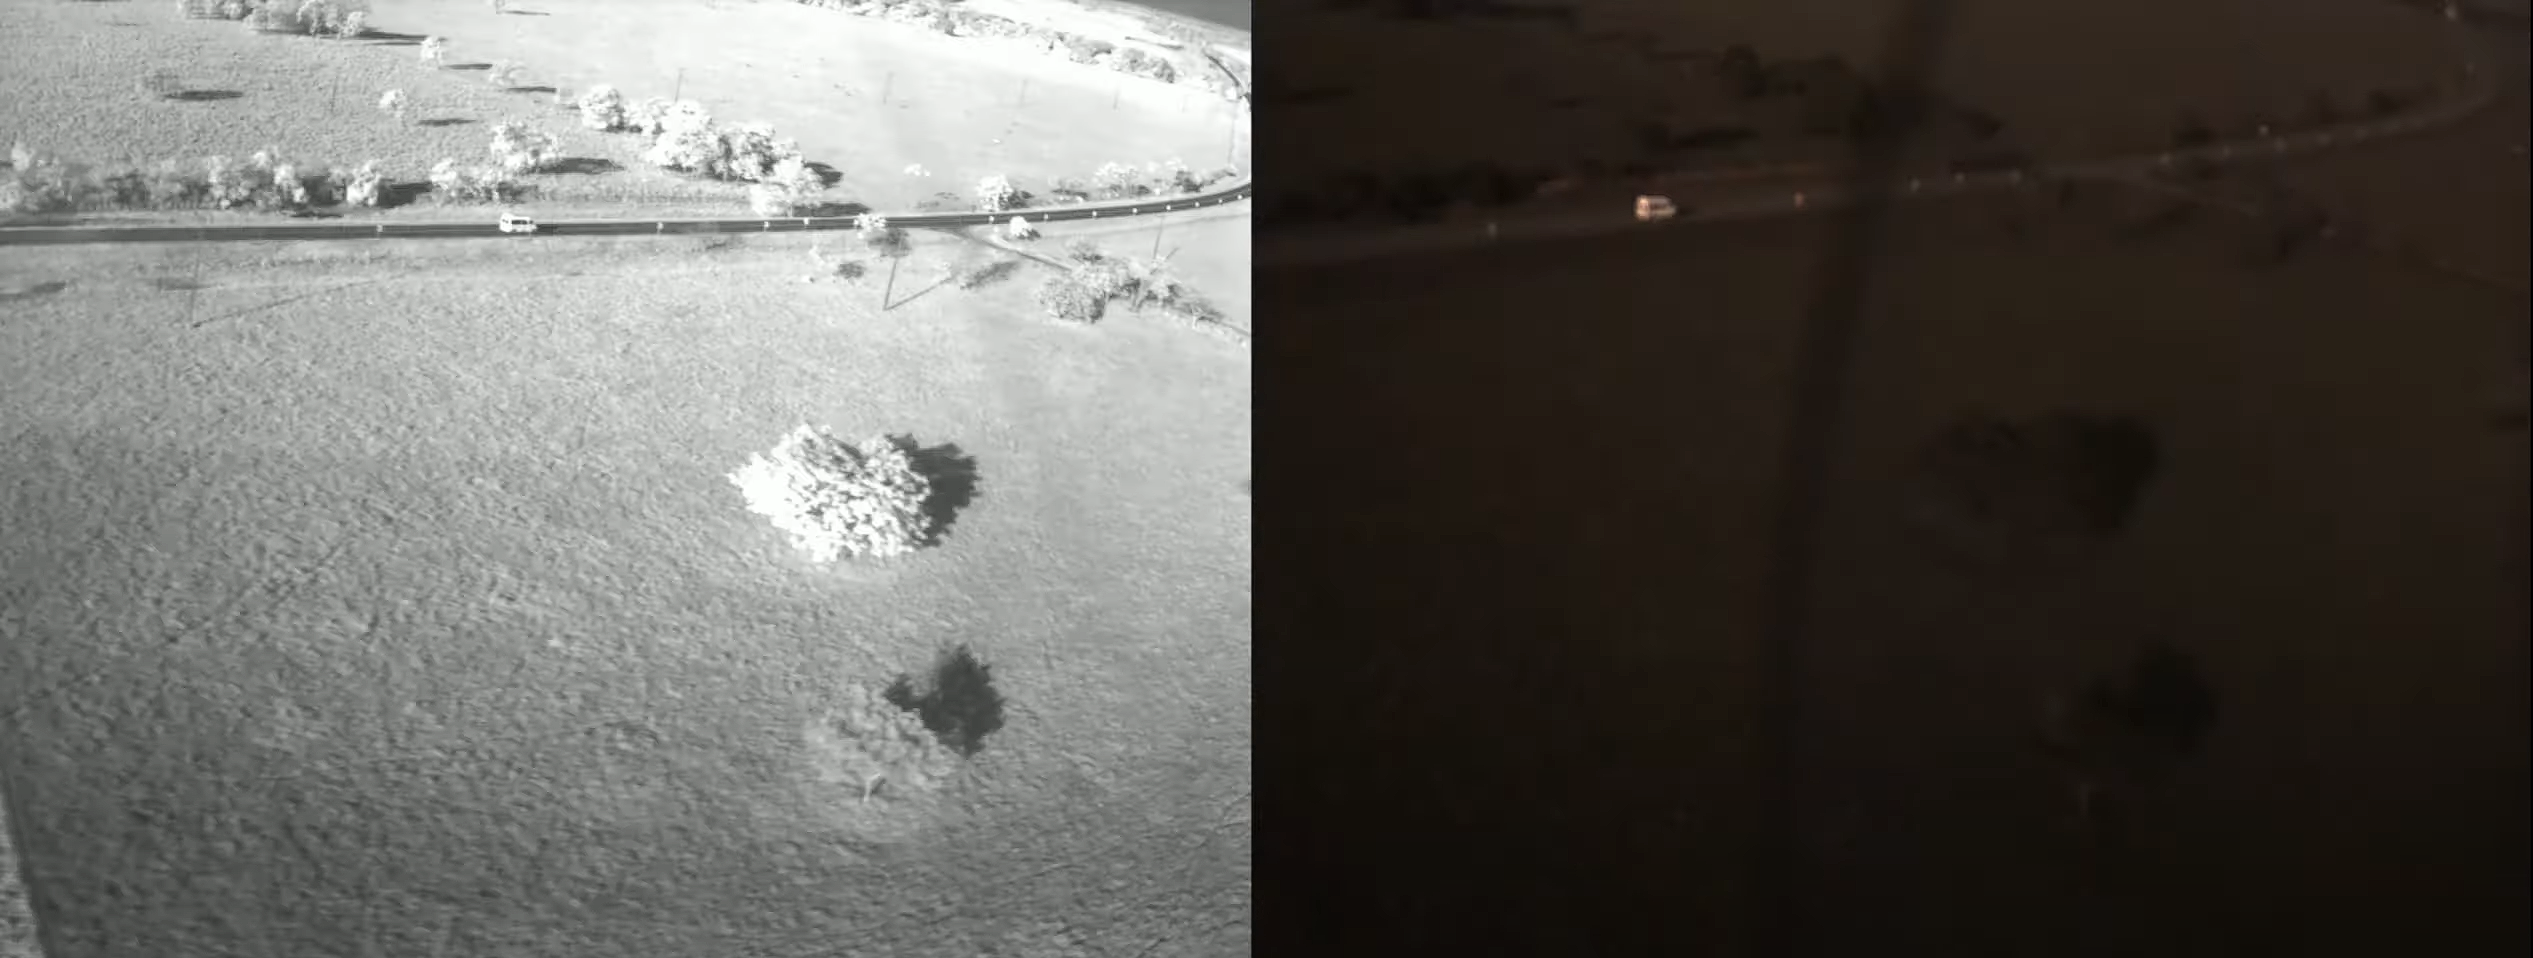
\includegraphics[width=0.9\textwidth]{Figures/C4/t2.png}
    \caption{Captura de video realizada durante prueba a bordo del avión de combate T-27 Tucano. A pesar de las maniobras con aceleraciones de hasta 4g, el sistema \textit{QBee} logró registrar imágenes de forma autónoma y estable. Las condiciones de iluminación ambiental no erán las más adecuadas debido a la hora del día (proximadamente las 6 pm).}
    \label{fig:prueba_tucano}
    \end{figure}
    

\section{Caracterización de las cámaras}
%---------------------------------------------------------------
     %===============================================================
     \subsection{Resultados de la caracterización del campo de visión (FOV)}
     \label{sec:fov_resultados}
     %===============================================================
     
     Para validar el campo de visión de los sistemas ópticos seleccionados (Sistema 7 VIS y Sistema 6 NIR), se realizaron mediciones de FOV horizontal (H) y vertical (V) a tres distancias de trabajo (\(\mathrm{WD}\)) empleando la carta de prueba ISO 12233. A continuación se presentan los resultados obtenidos.\\
     
     La Figura \ref{fig:fov_montage} muestra las 12 capturas originales (3 filas × 4 columnas) utilizadas para determinar experimentalmente el FOV. Cada fila corresponde a una distancia de trabajo distinta; las dos primeras columnas son las mediciones H y V de VIS (Sistema 7) y las dos últimas, las de NIR (Sistema 6).
     
     \begin{figure}[H]
       \centering
       \setlength{\tabcolsep}{2pt}
       \renewcommand{\arraystretch}{0}
       \begin{tabular}{cccc}
         \multicolumn{2}{c}{\small NIR – Sistema 6} &
         \multicolumn{2}{c}{\small VIS – Sistema 7} \\
         H & V & H & V \\ 
 
         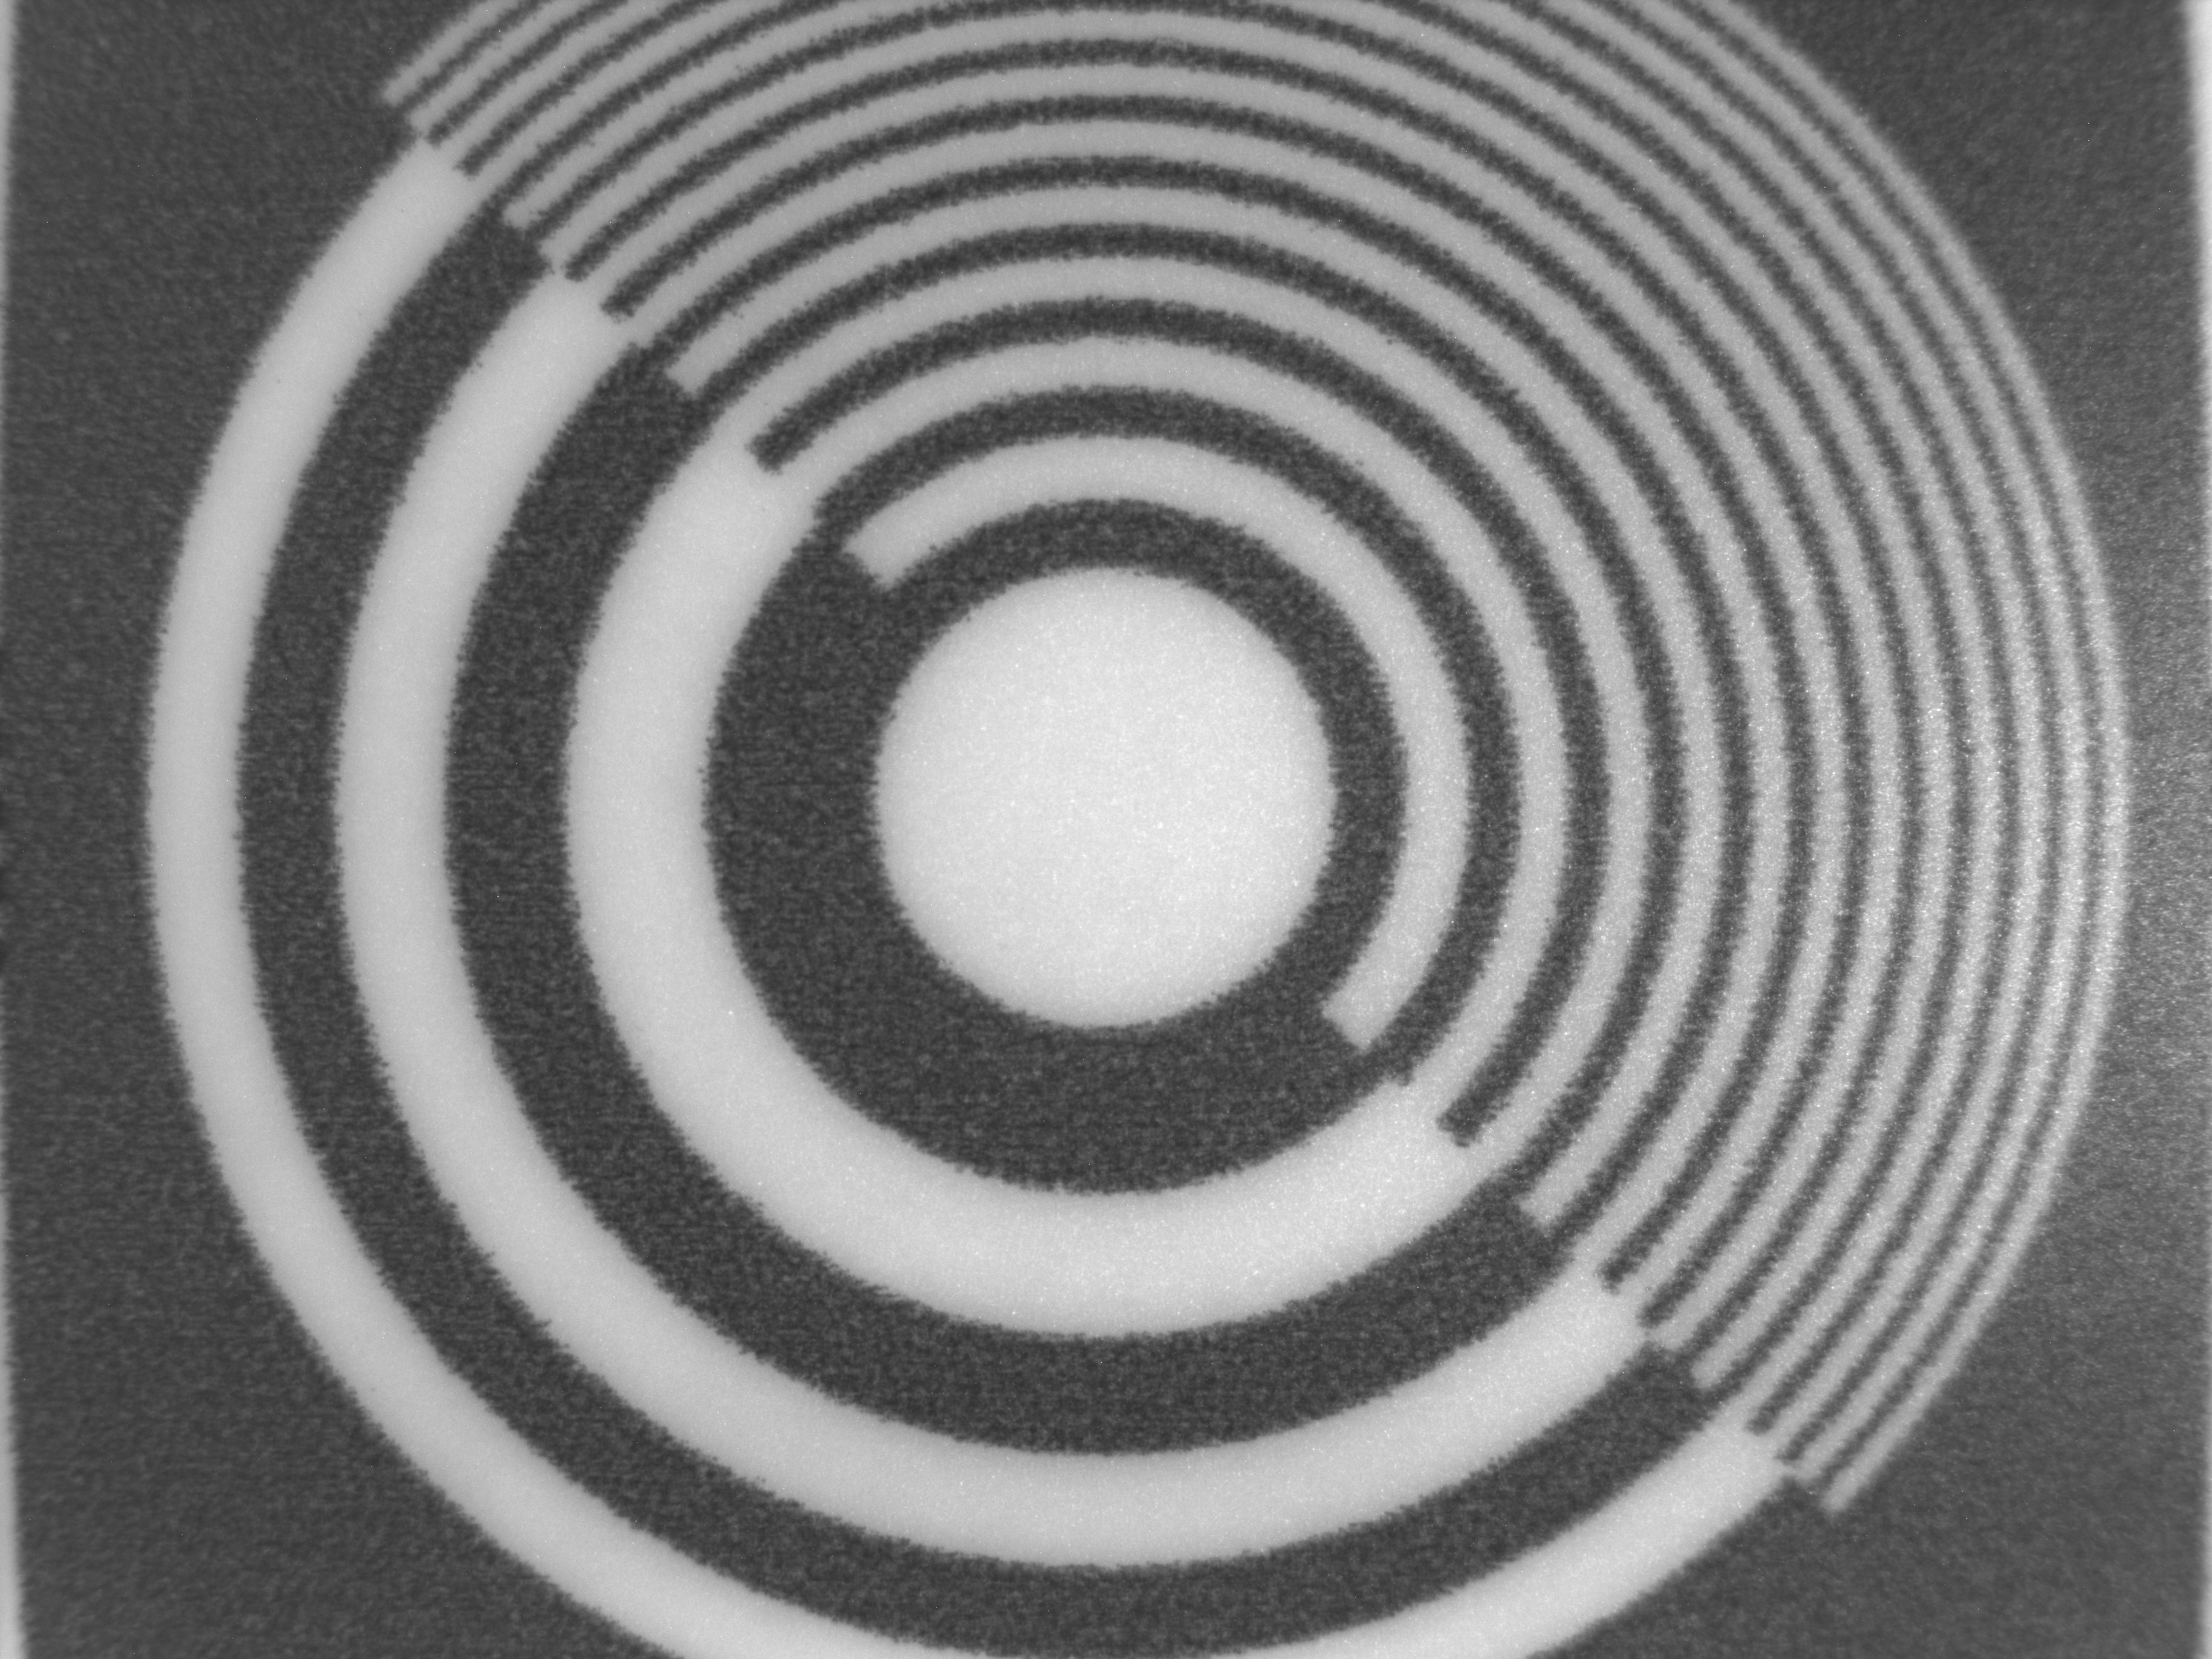
\includegraphics[width=.22\linewidth]{Figures/C4/FOV/NIR/H/7_1.png} &
         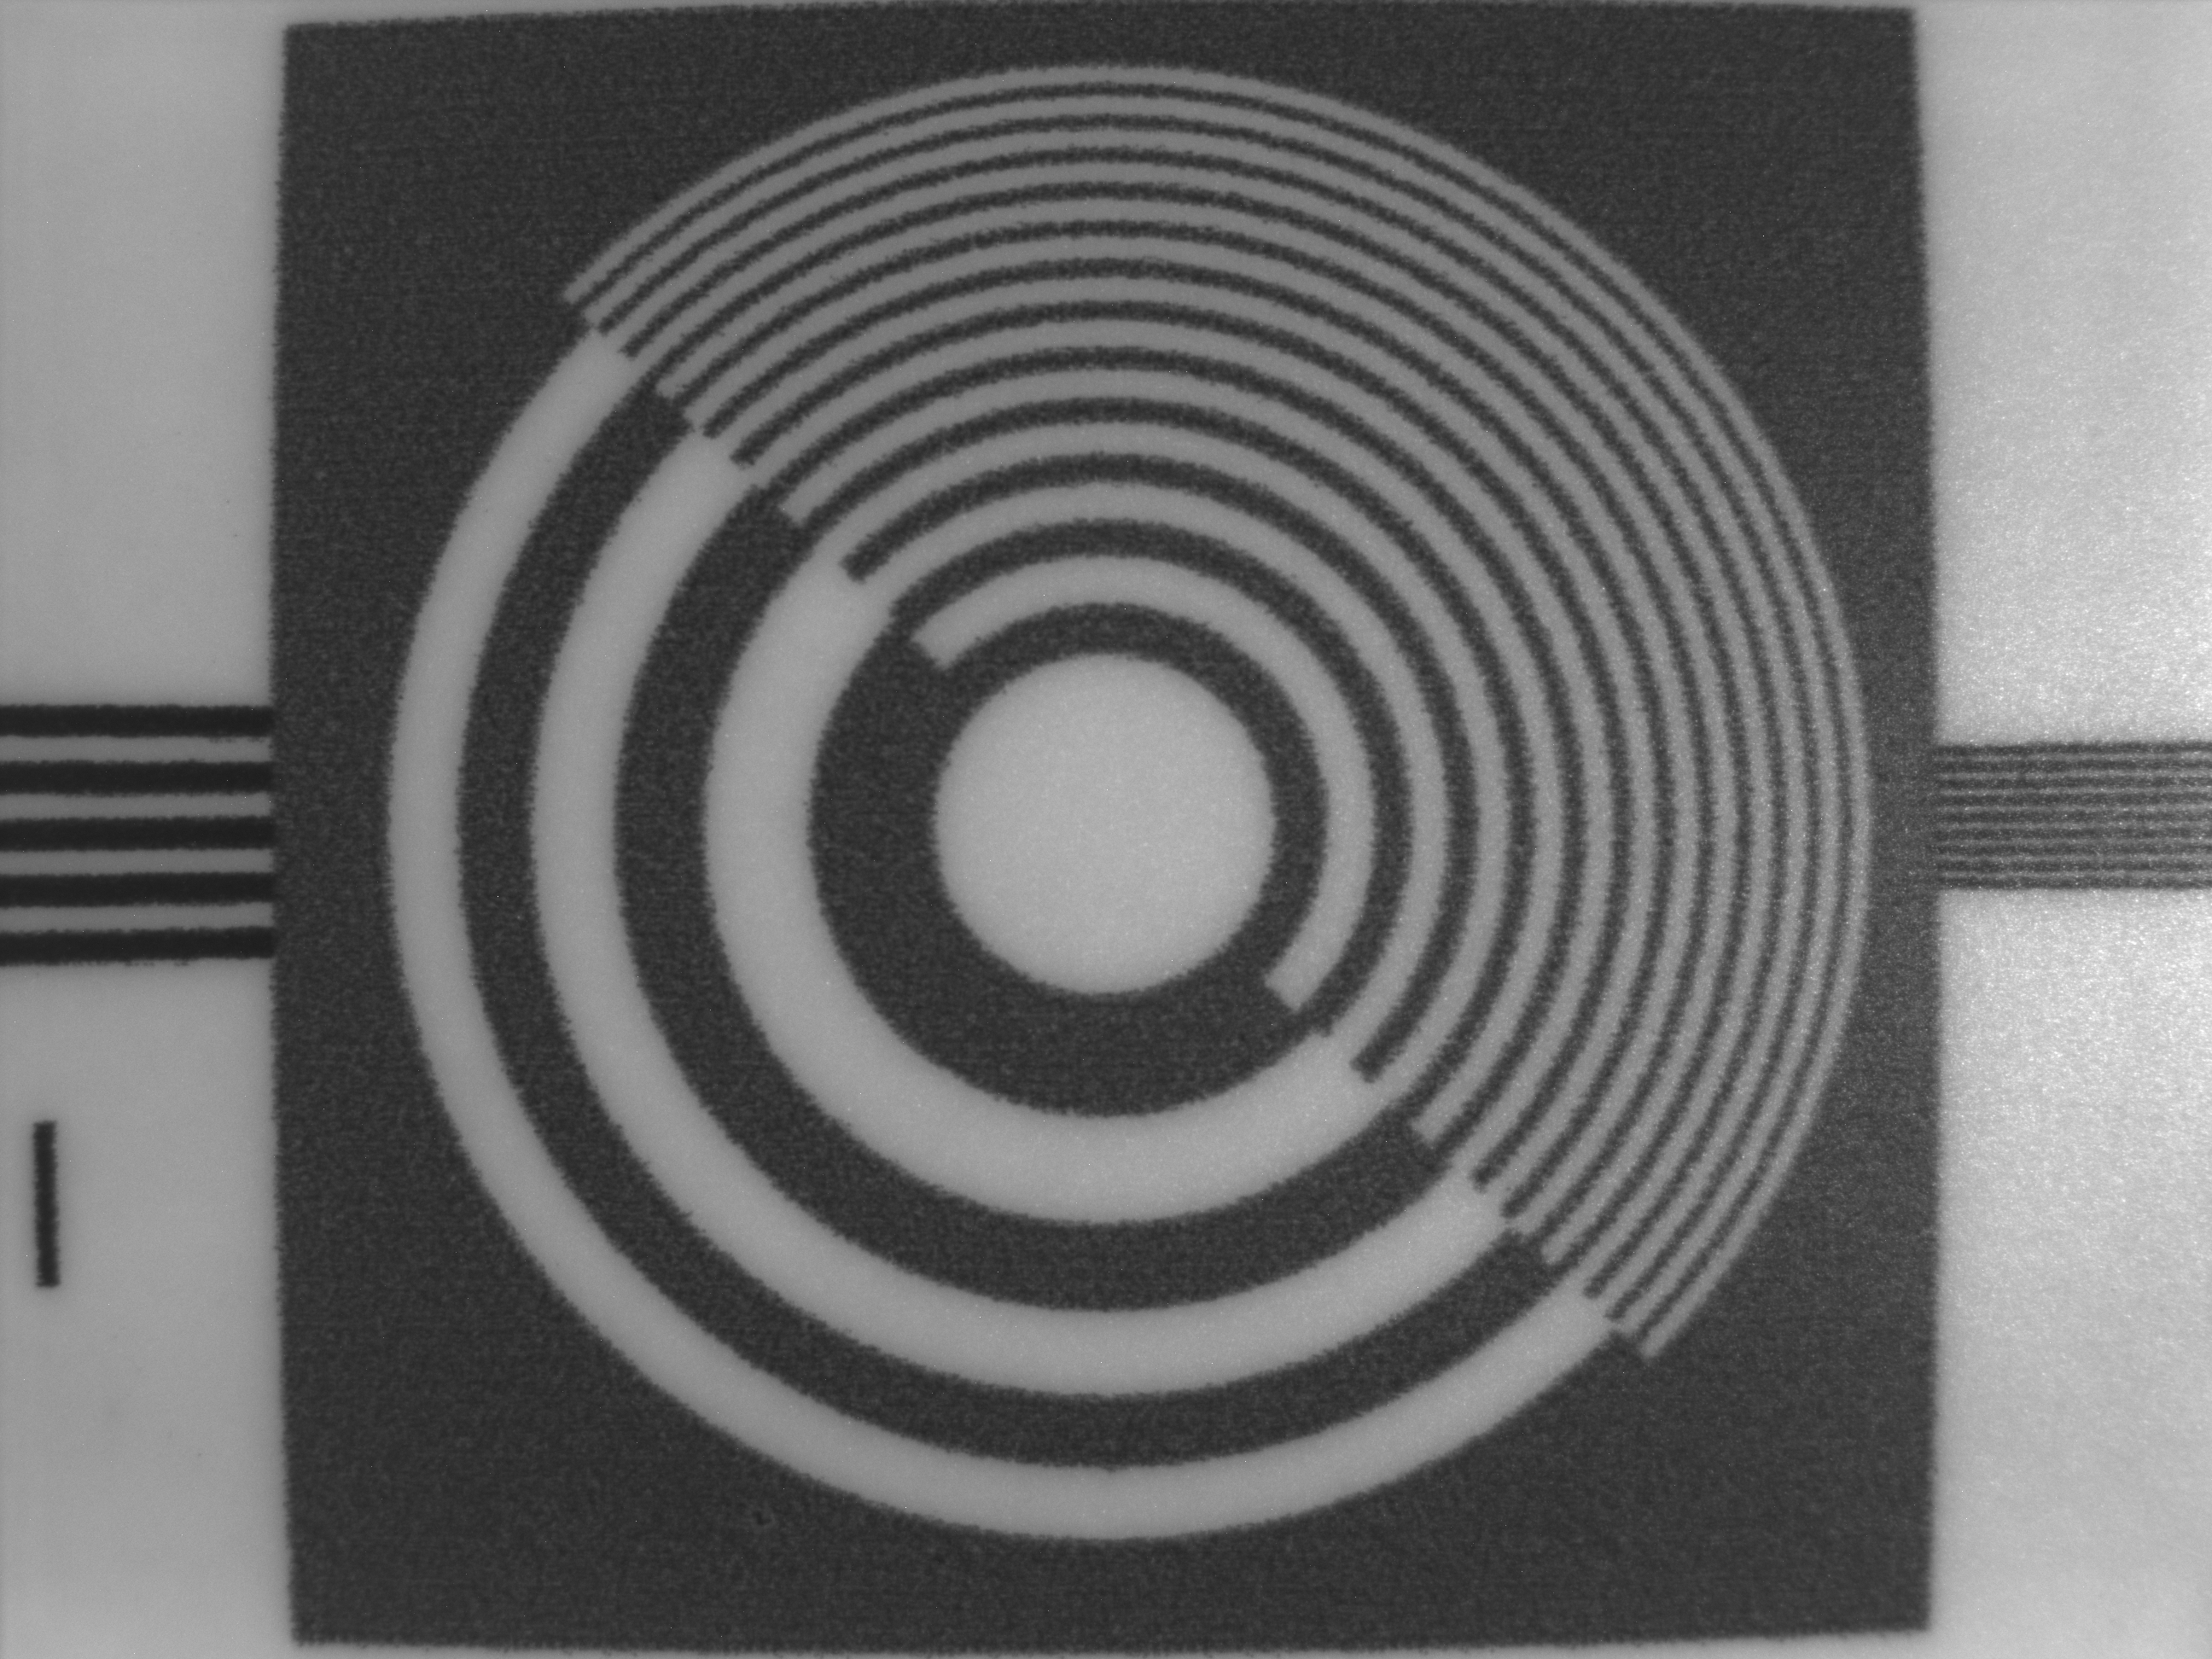
\includegraphics[width=.22\linewidth]{Figures/C4/FOV/NIR/V/8_7.png} &
         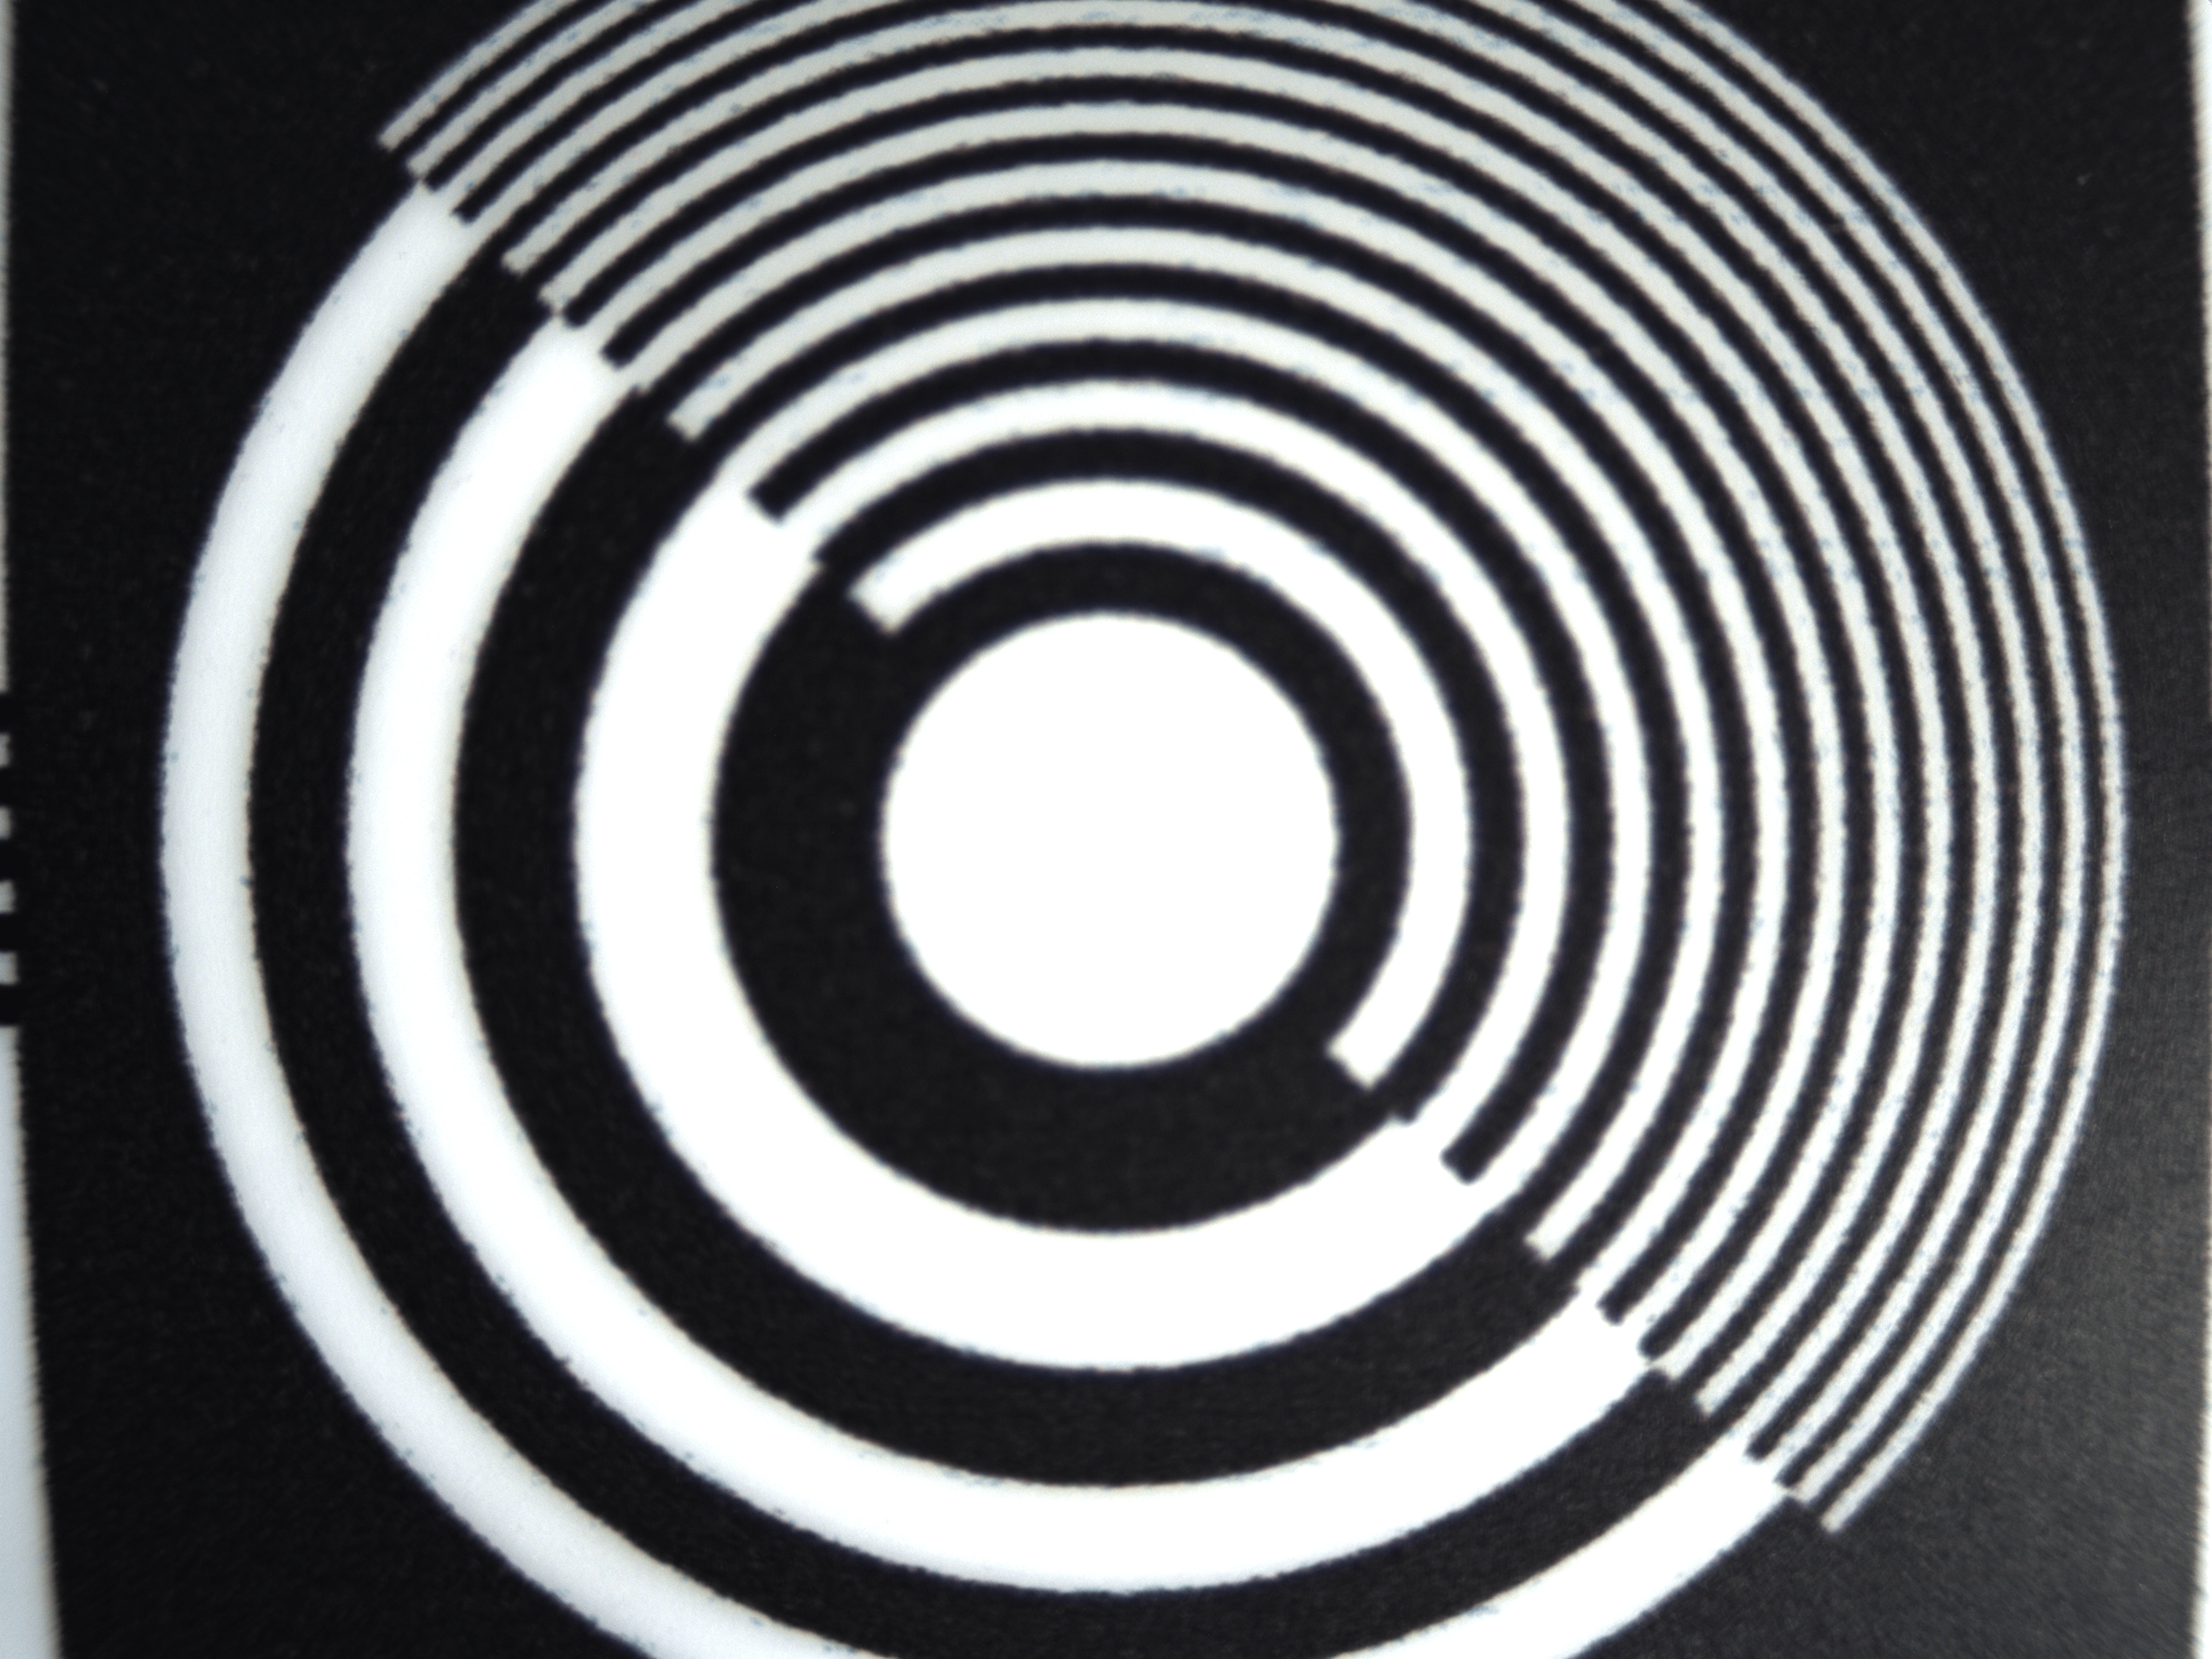
\includegraphics[width=.22\linewidth]{Figures/C4/FOV/VIS/H/9_2.png} &
         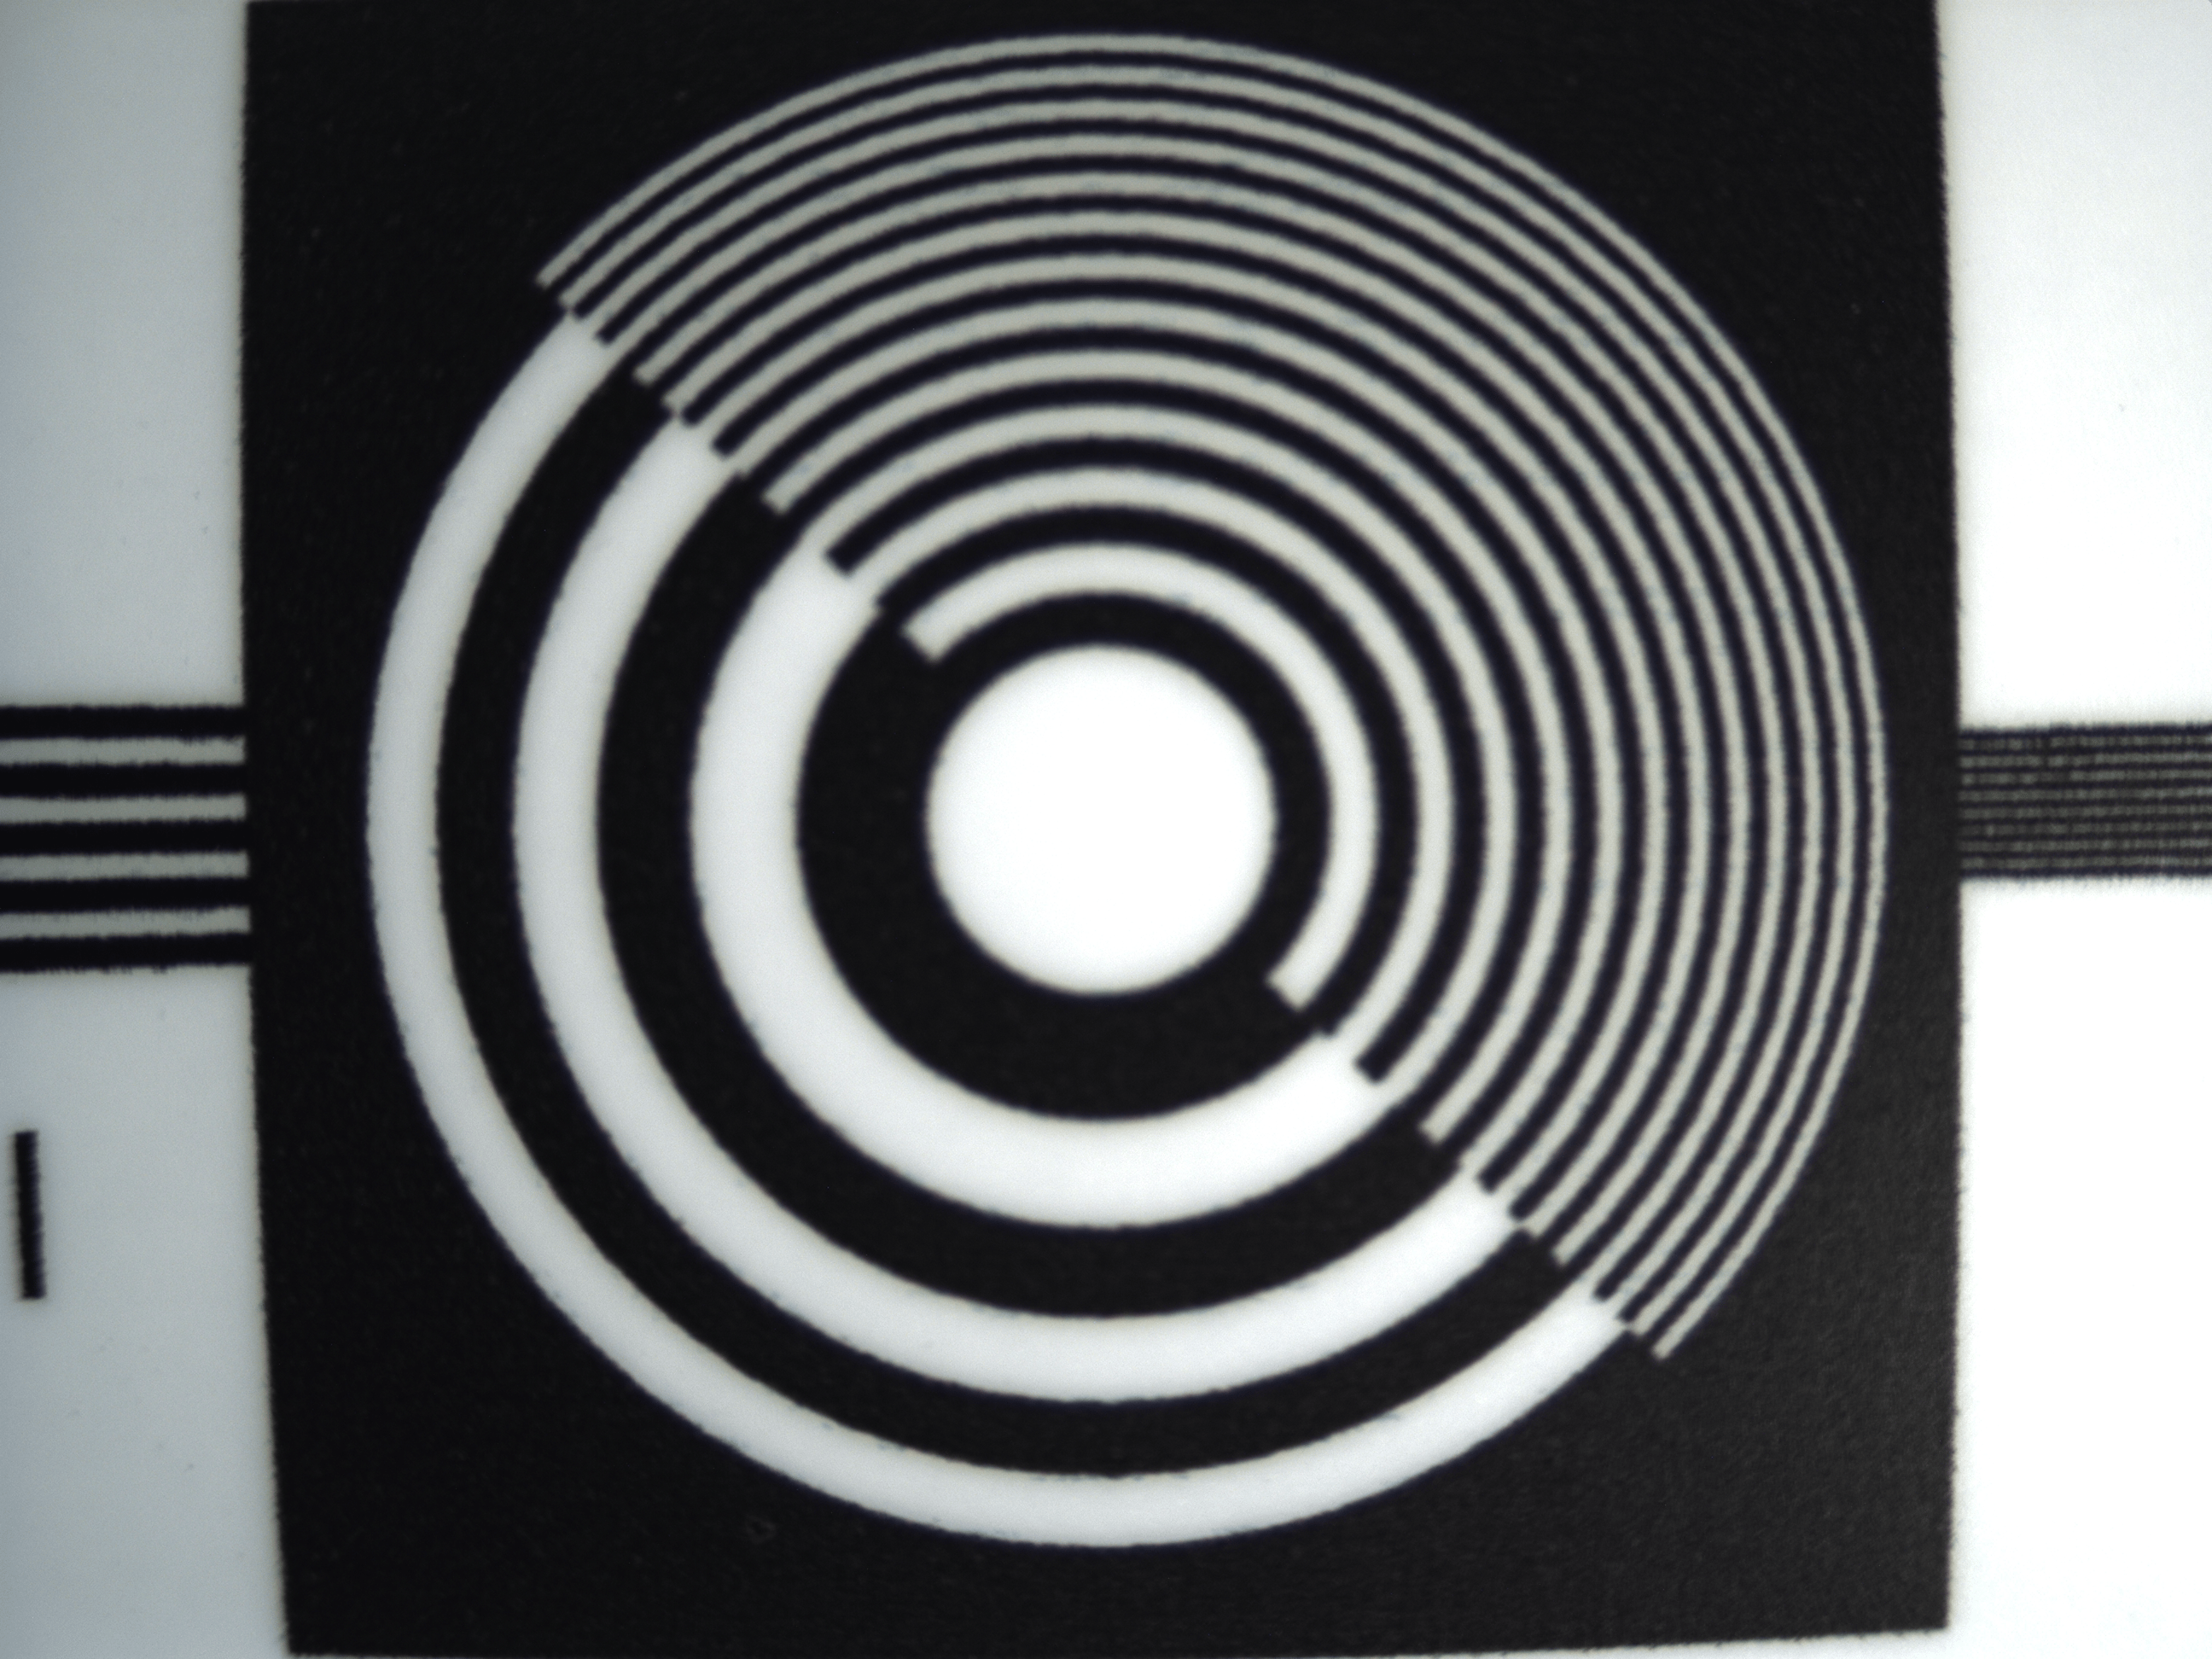
\includegraphics[width=.22\linewidth]{Figures/C4/FOV/VIS/V/10_7.png} \\
         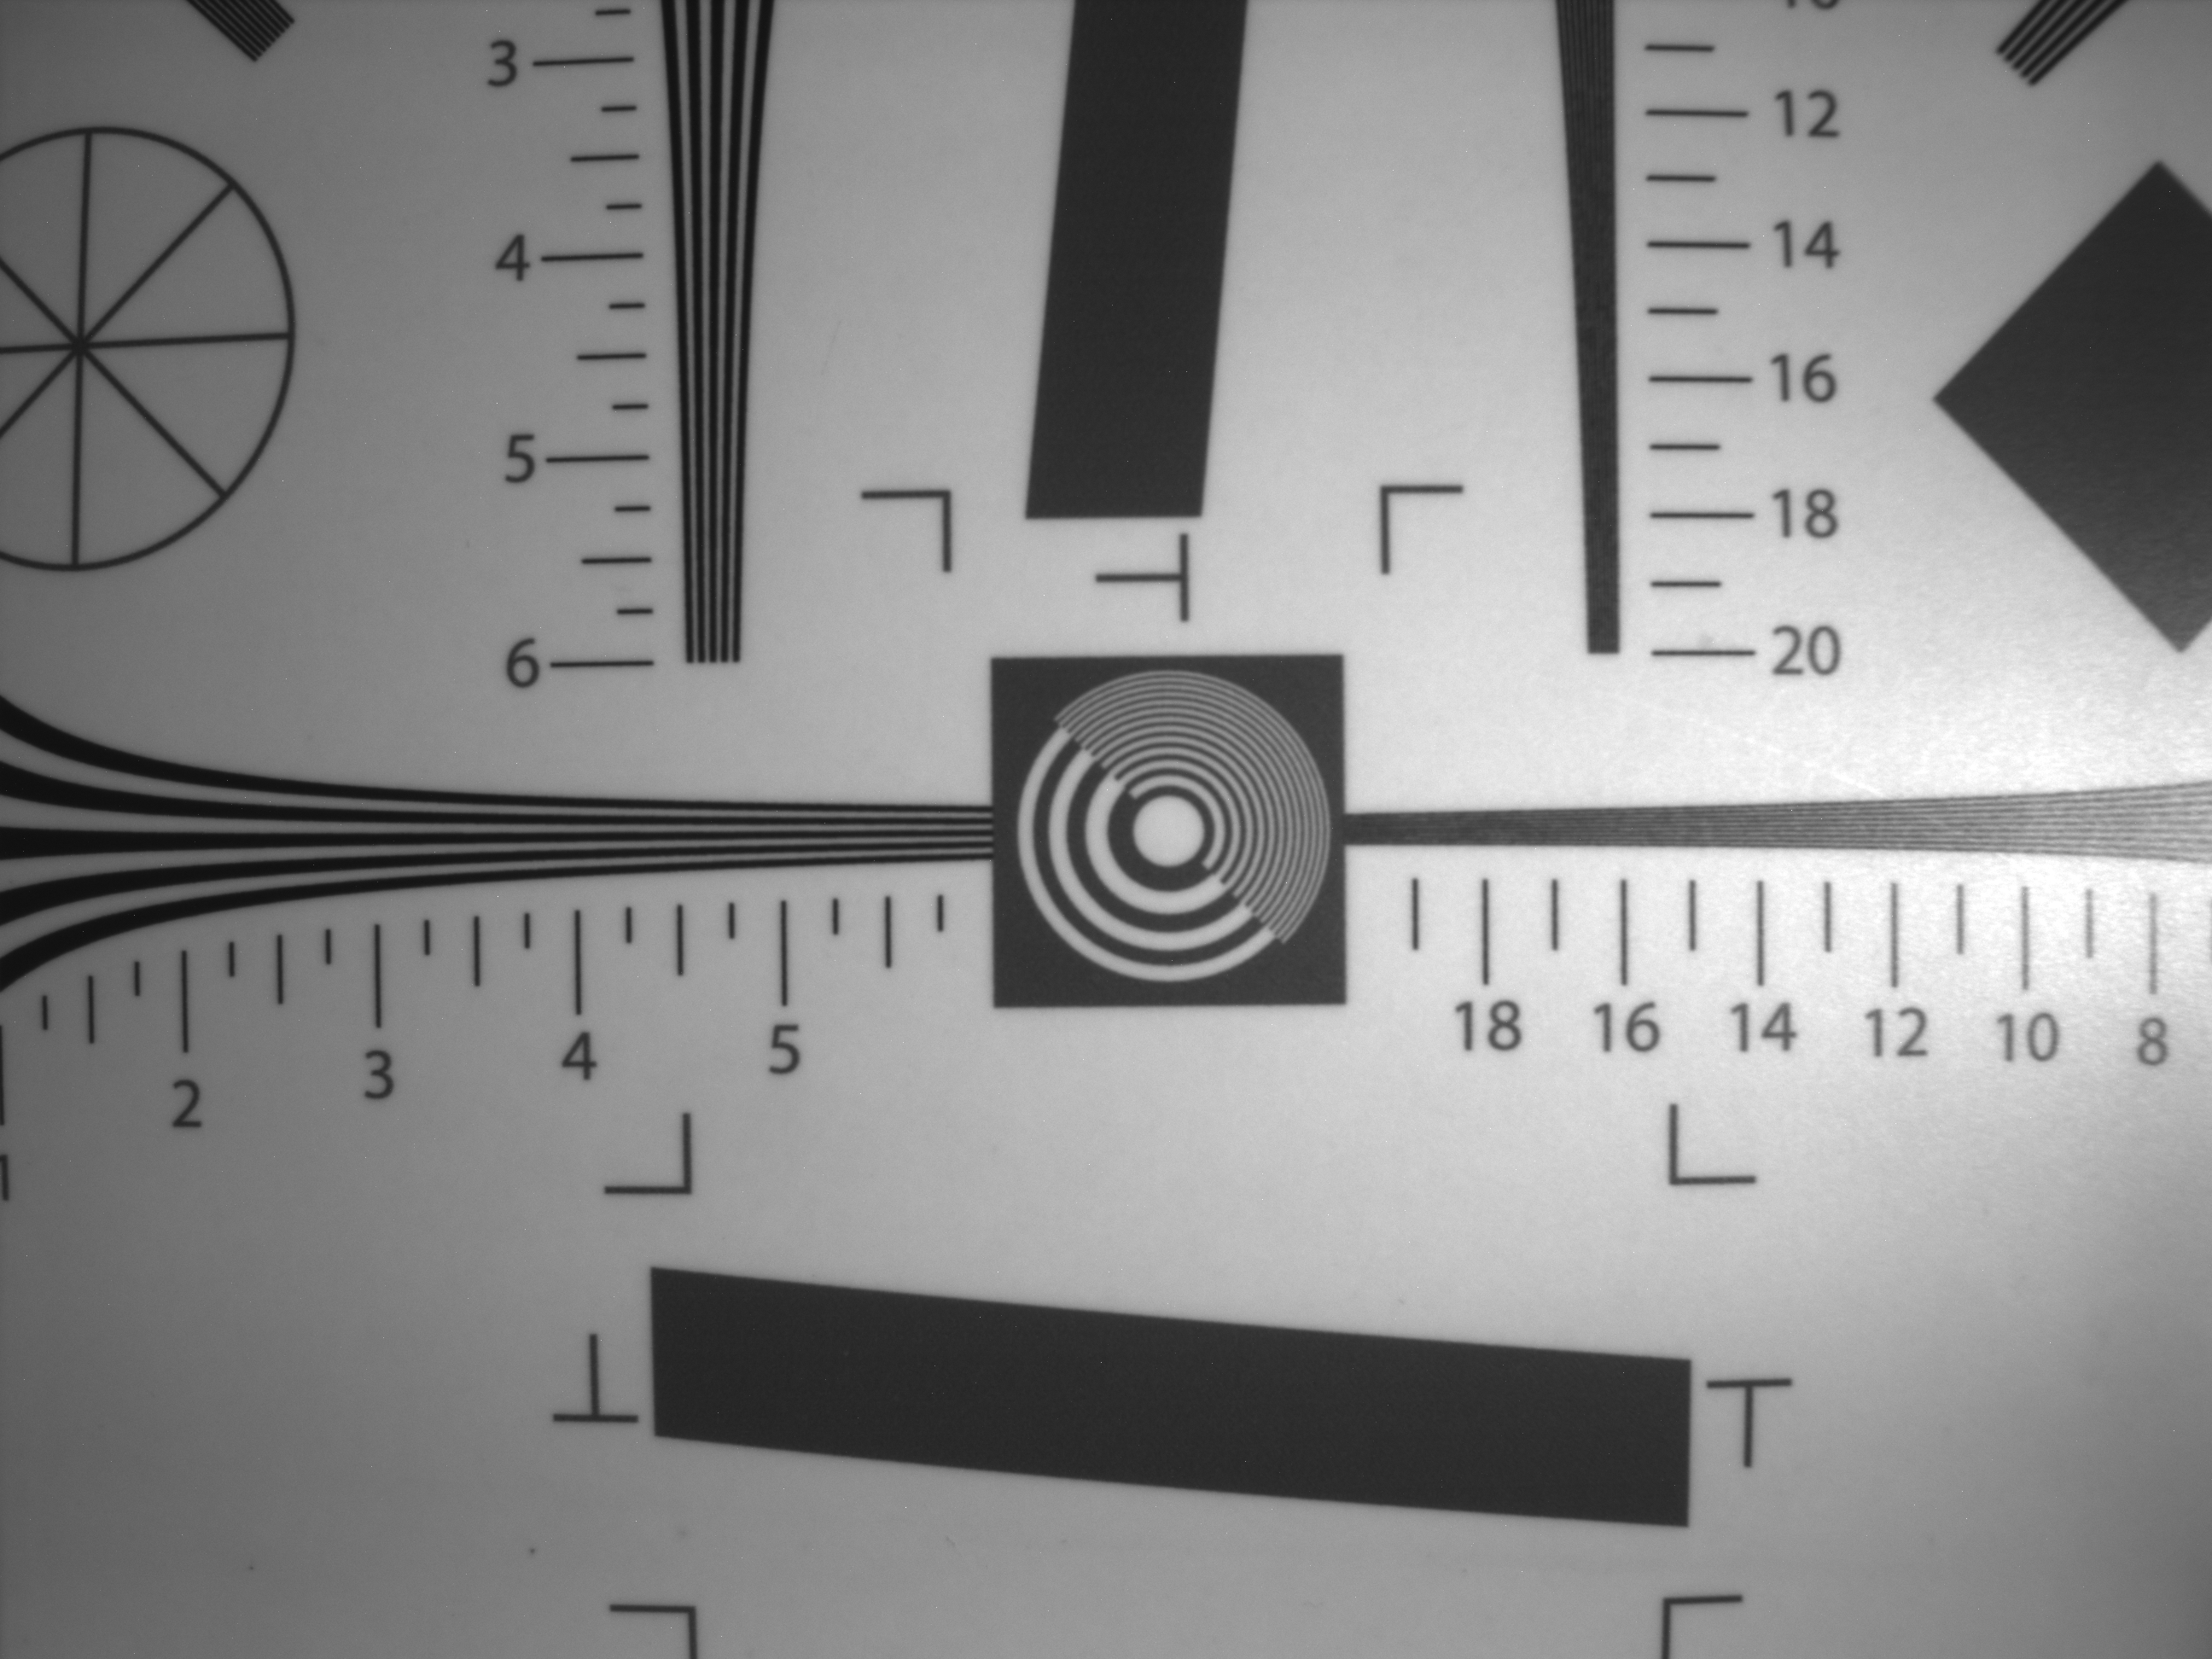
\includegraphics[width=.22\linewidth]{Figures/C4/FOV/NIR/H/33_1.png} &
         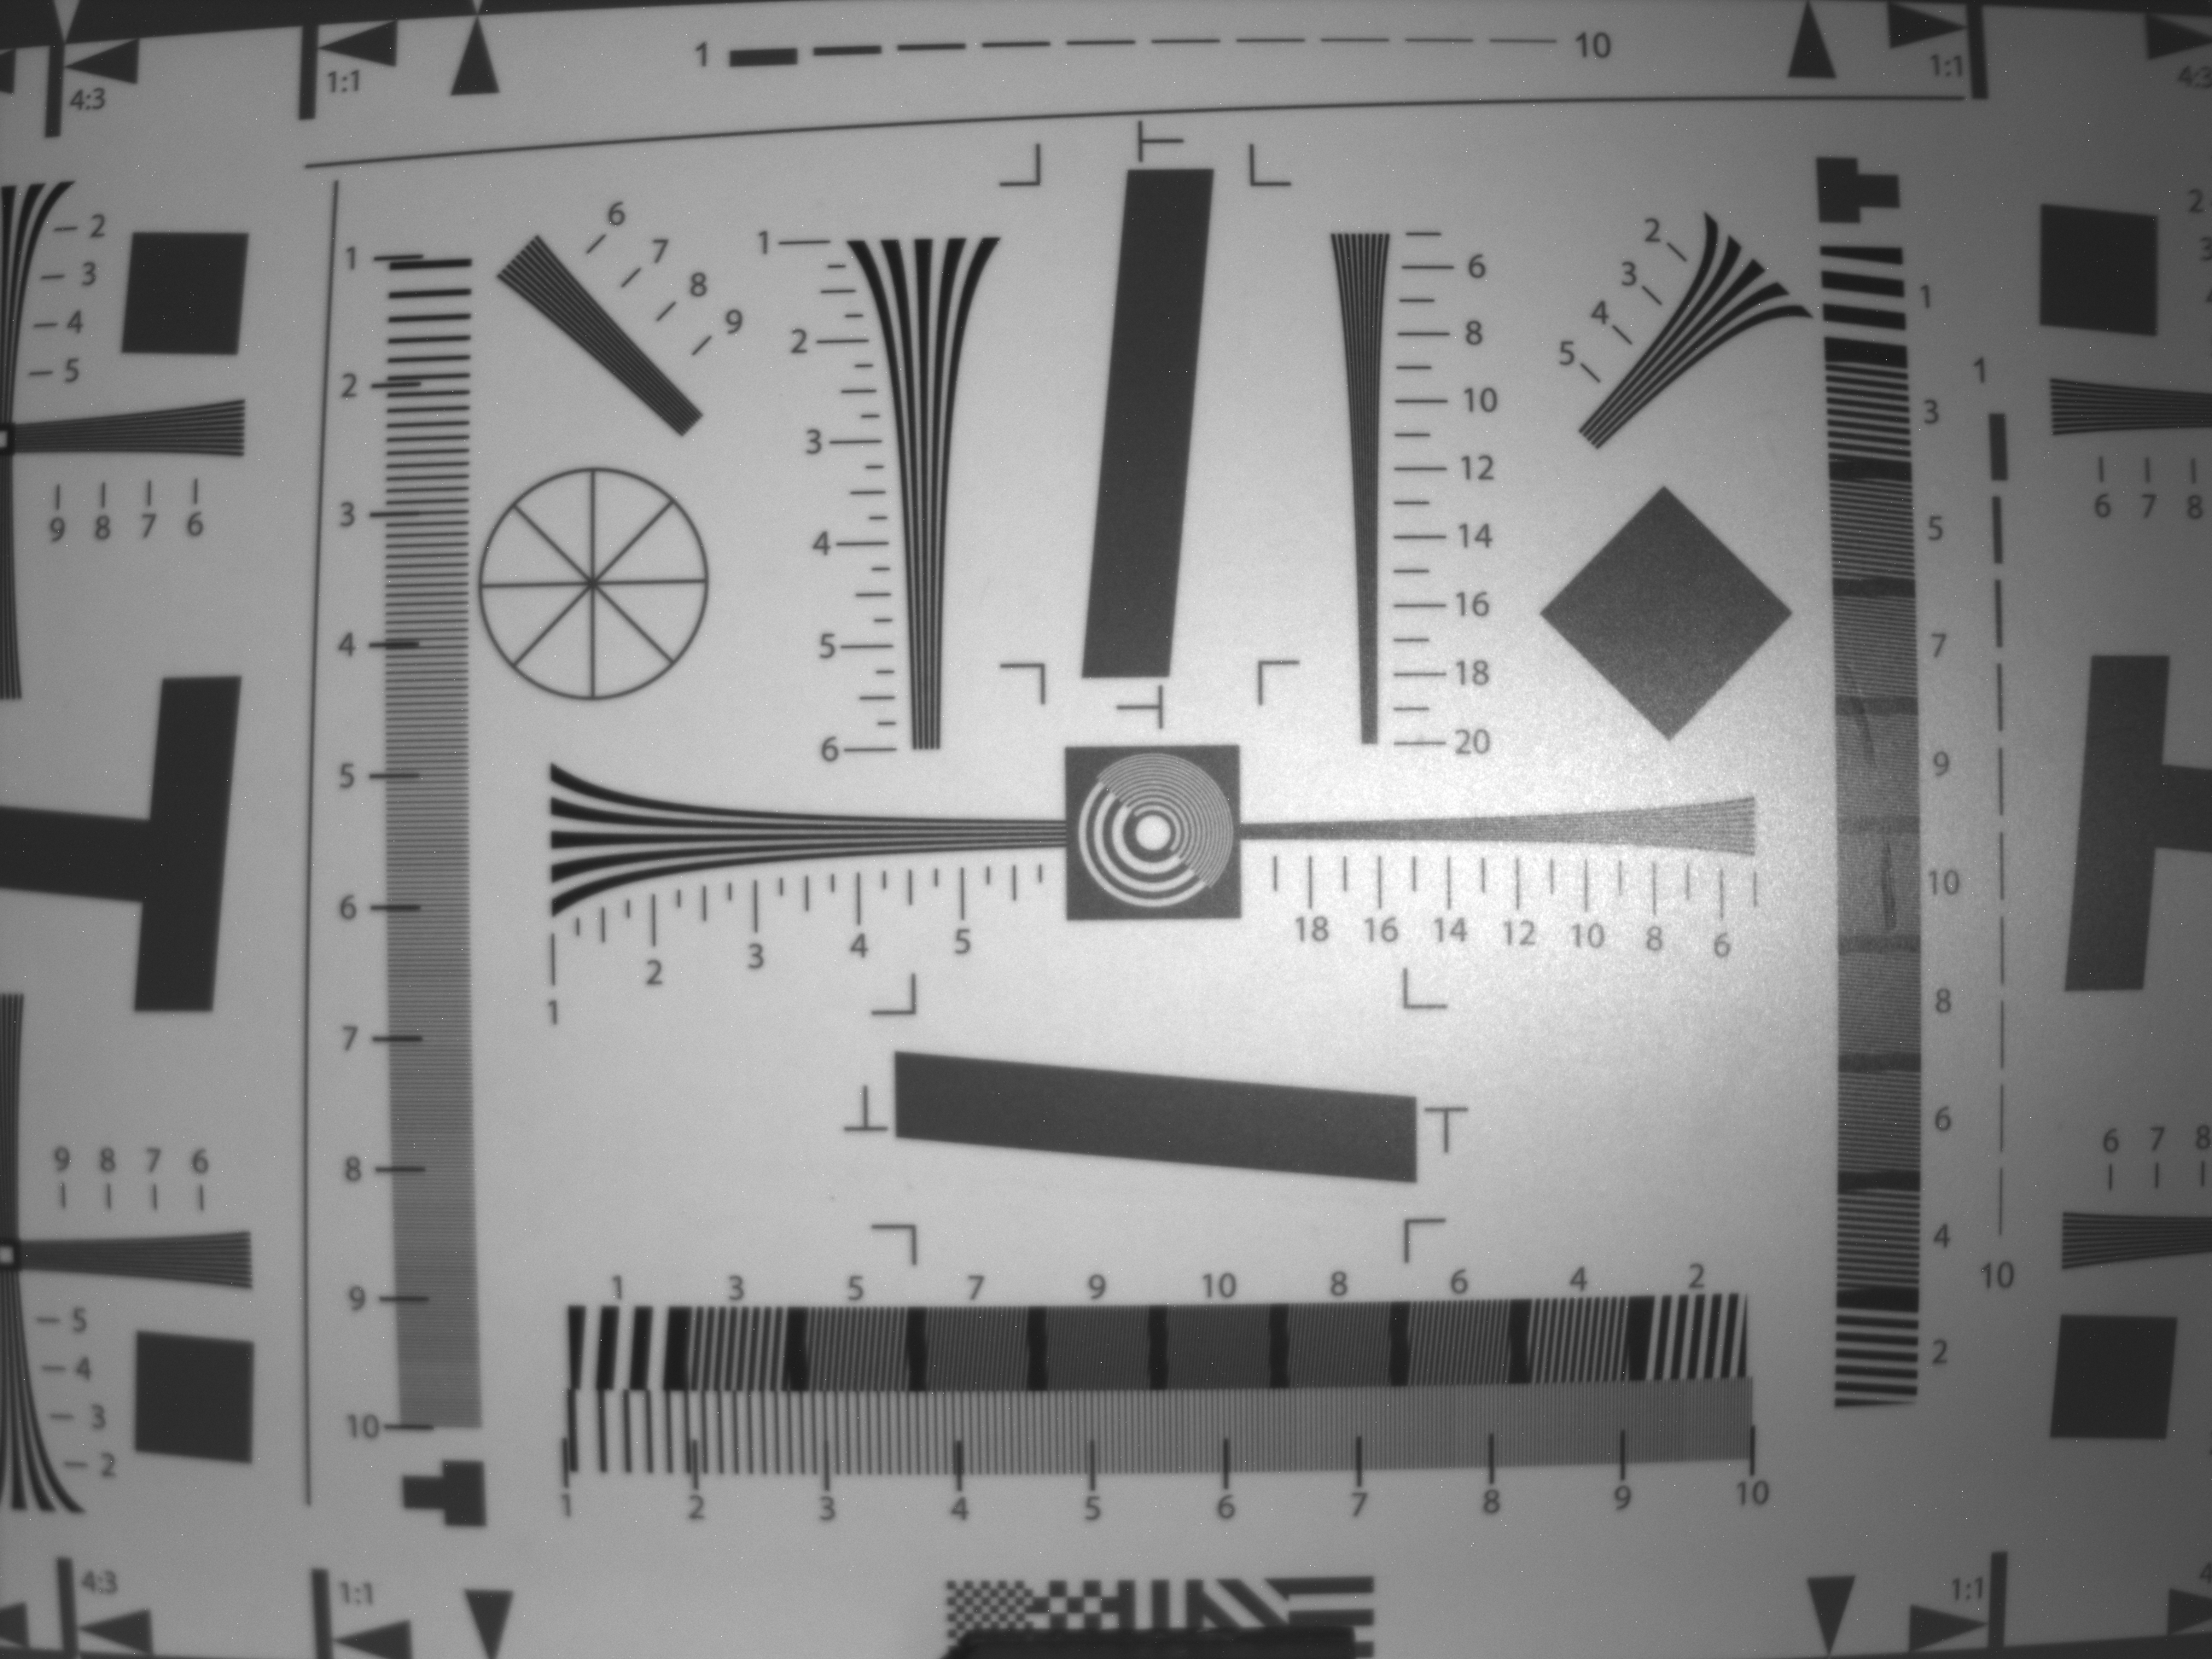
\includegraphics[trim= 6cm 6cm 6cm 6cm, clip, width=.22\linewidth]{Figures/C4/FOV/NIR/V/65.png} & % TOCLIP
         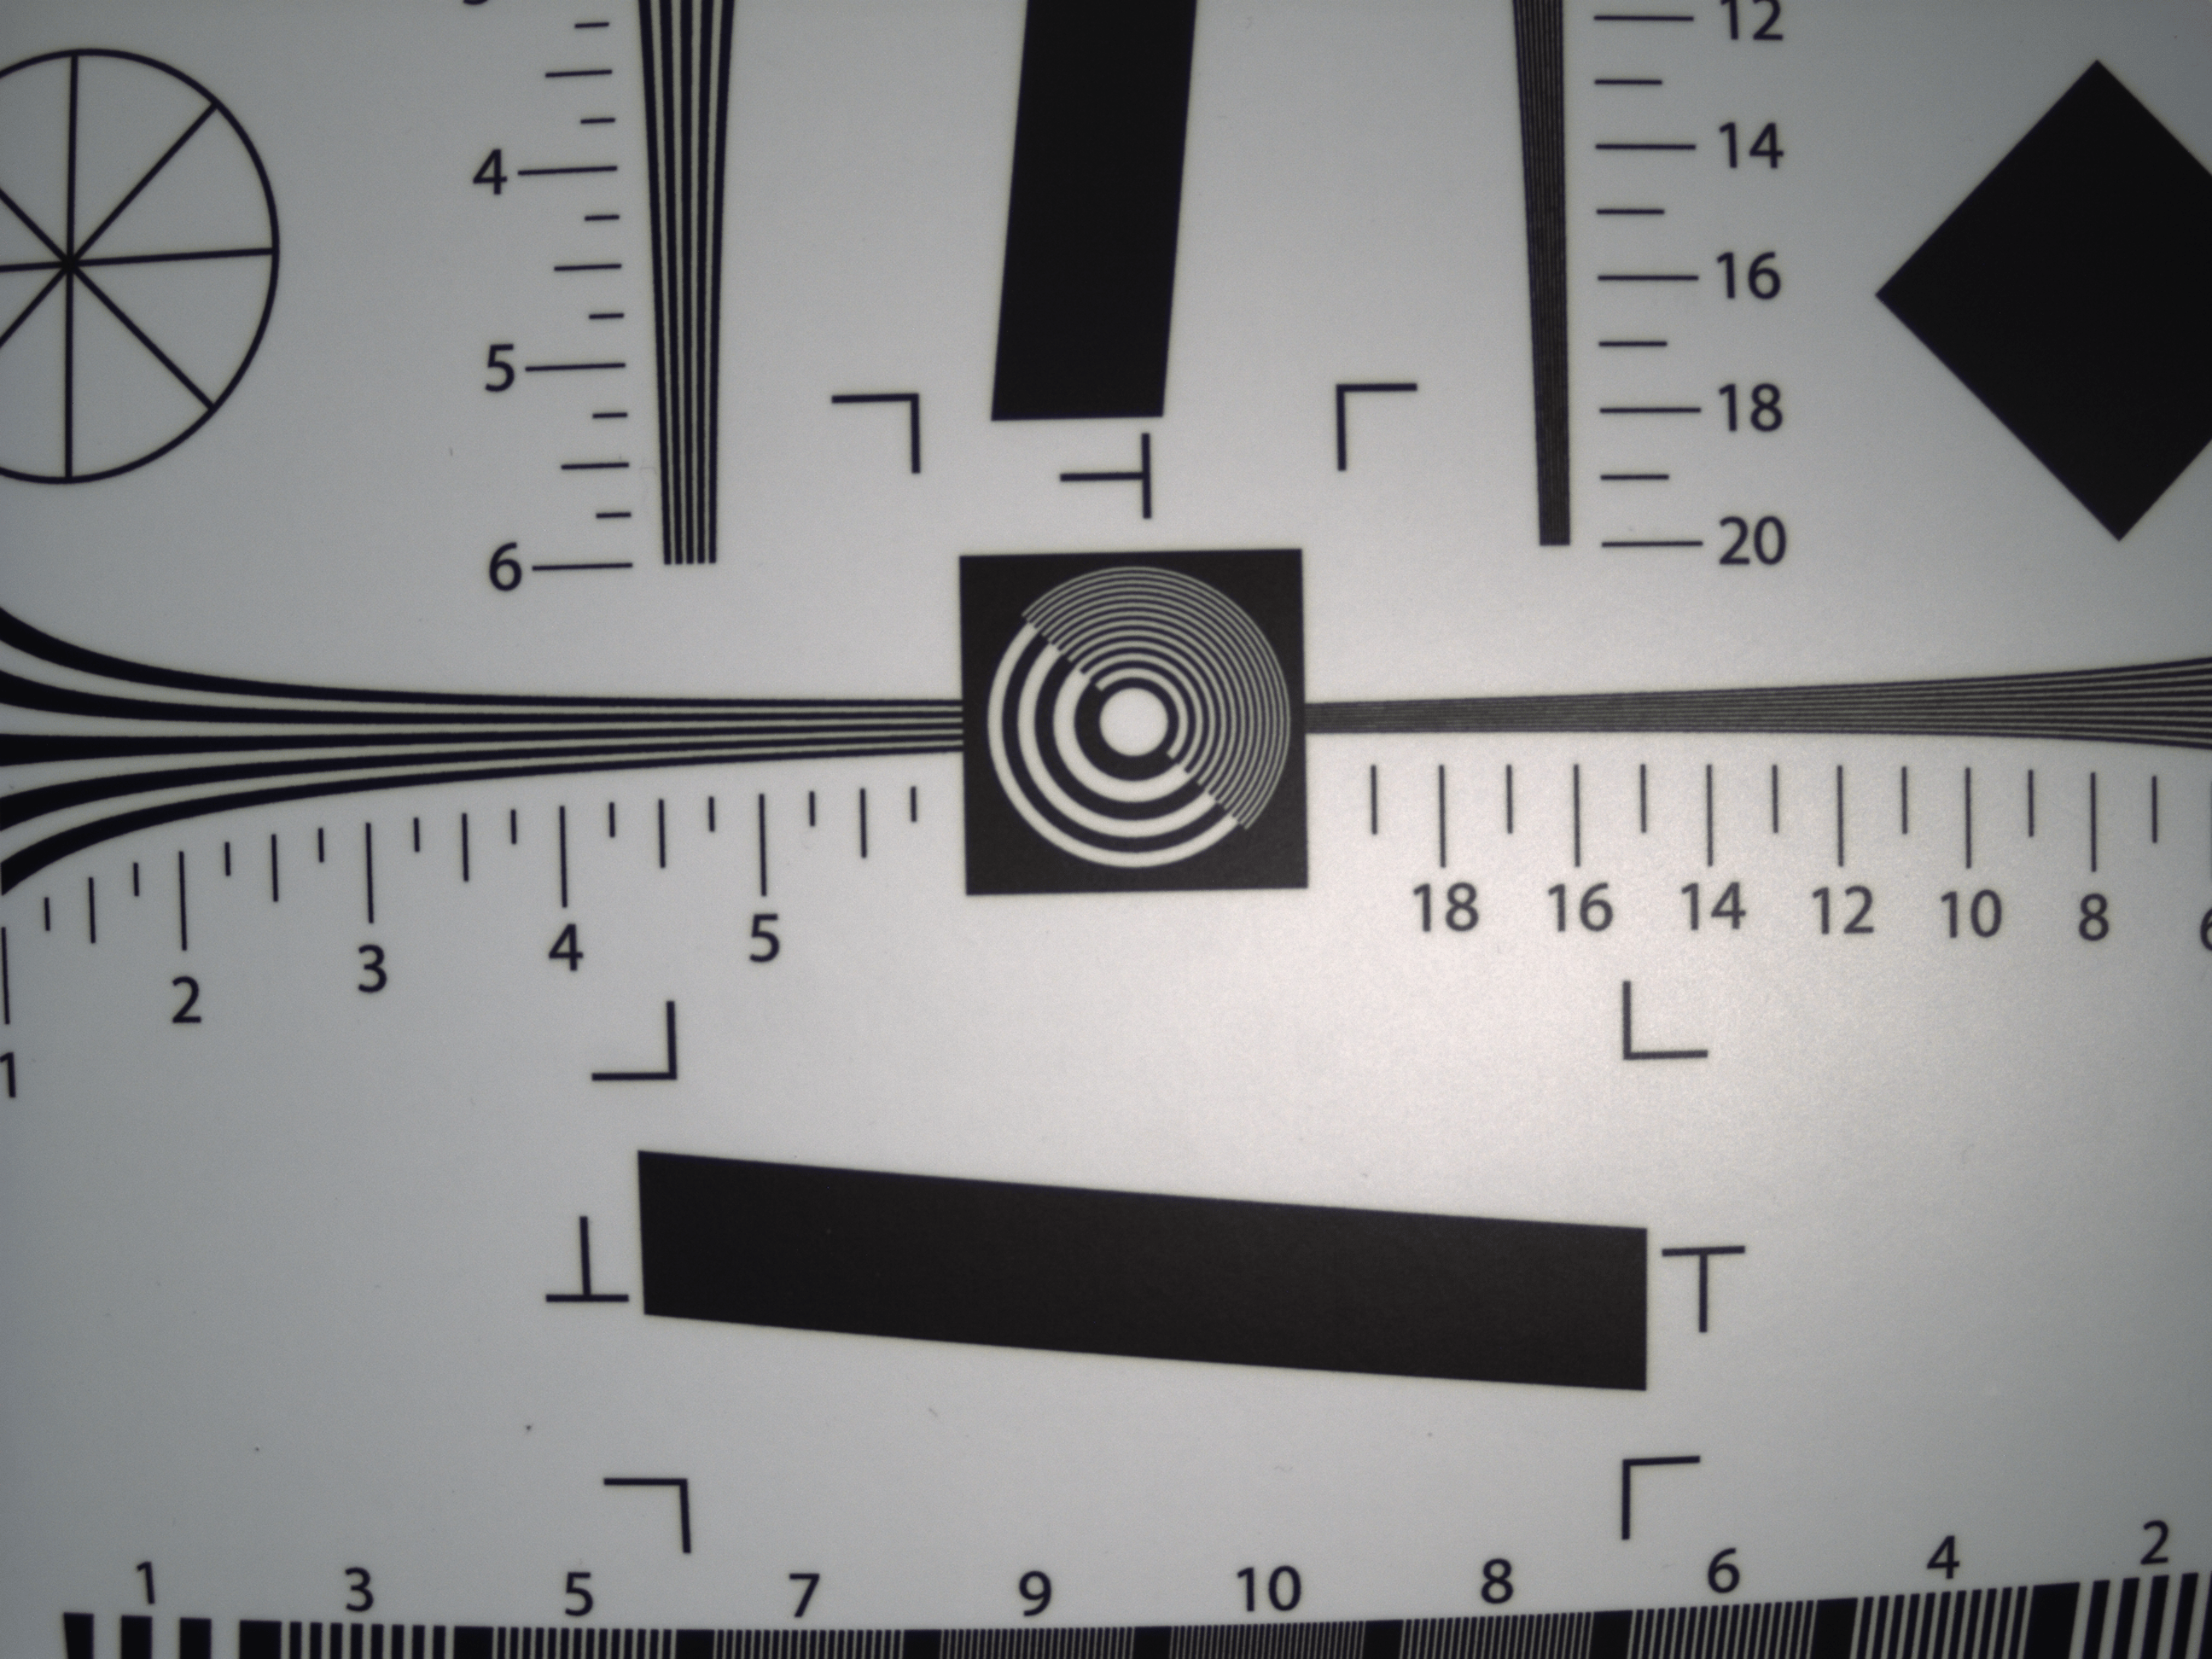
\includegraphics[width=.22\linewidth]{Figures/C4/FOV/VIS/H/37_8.png} &
         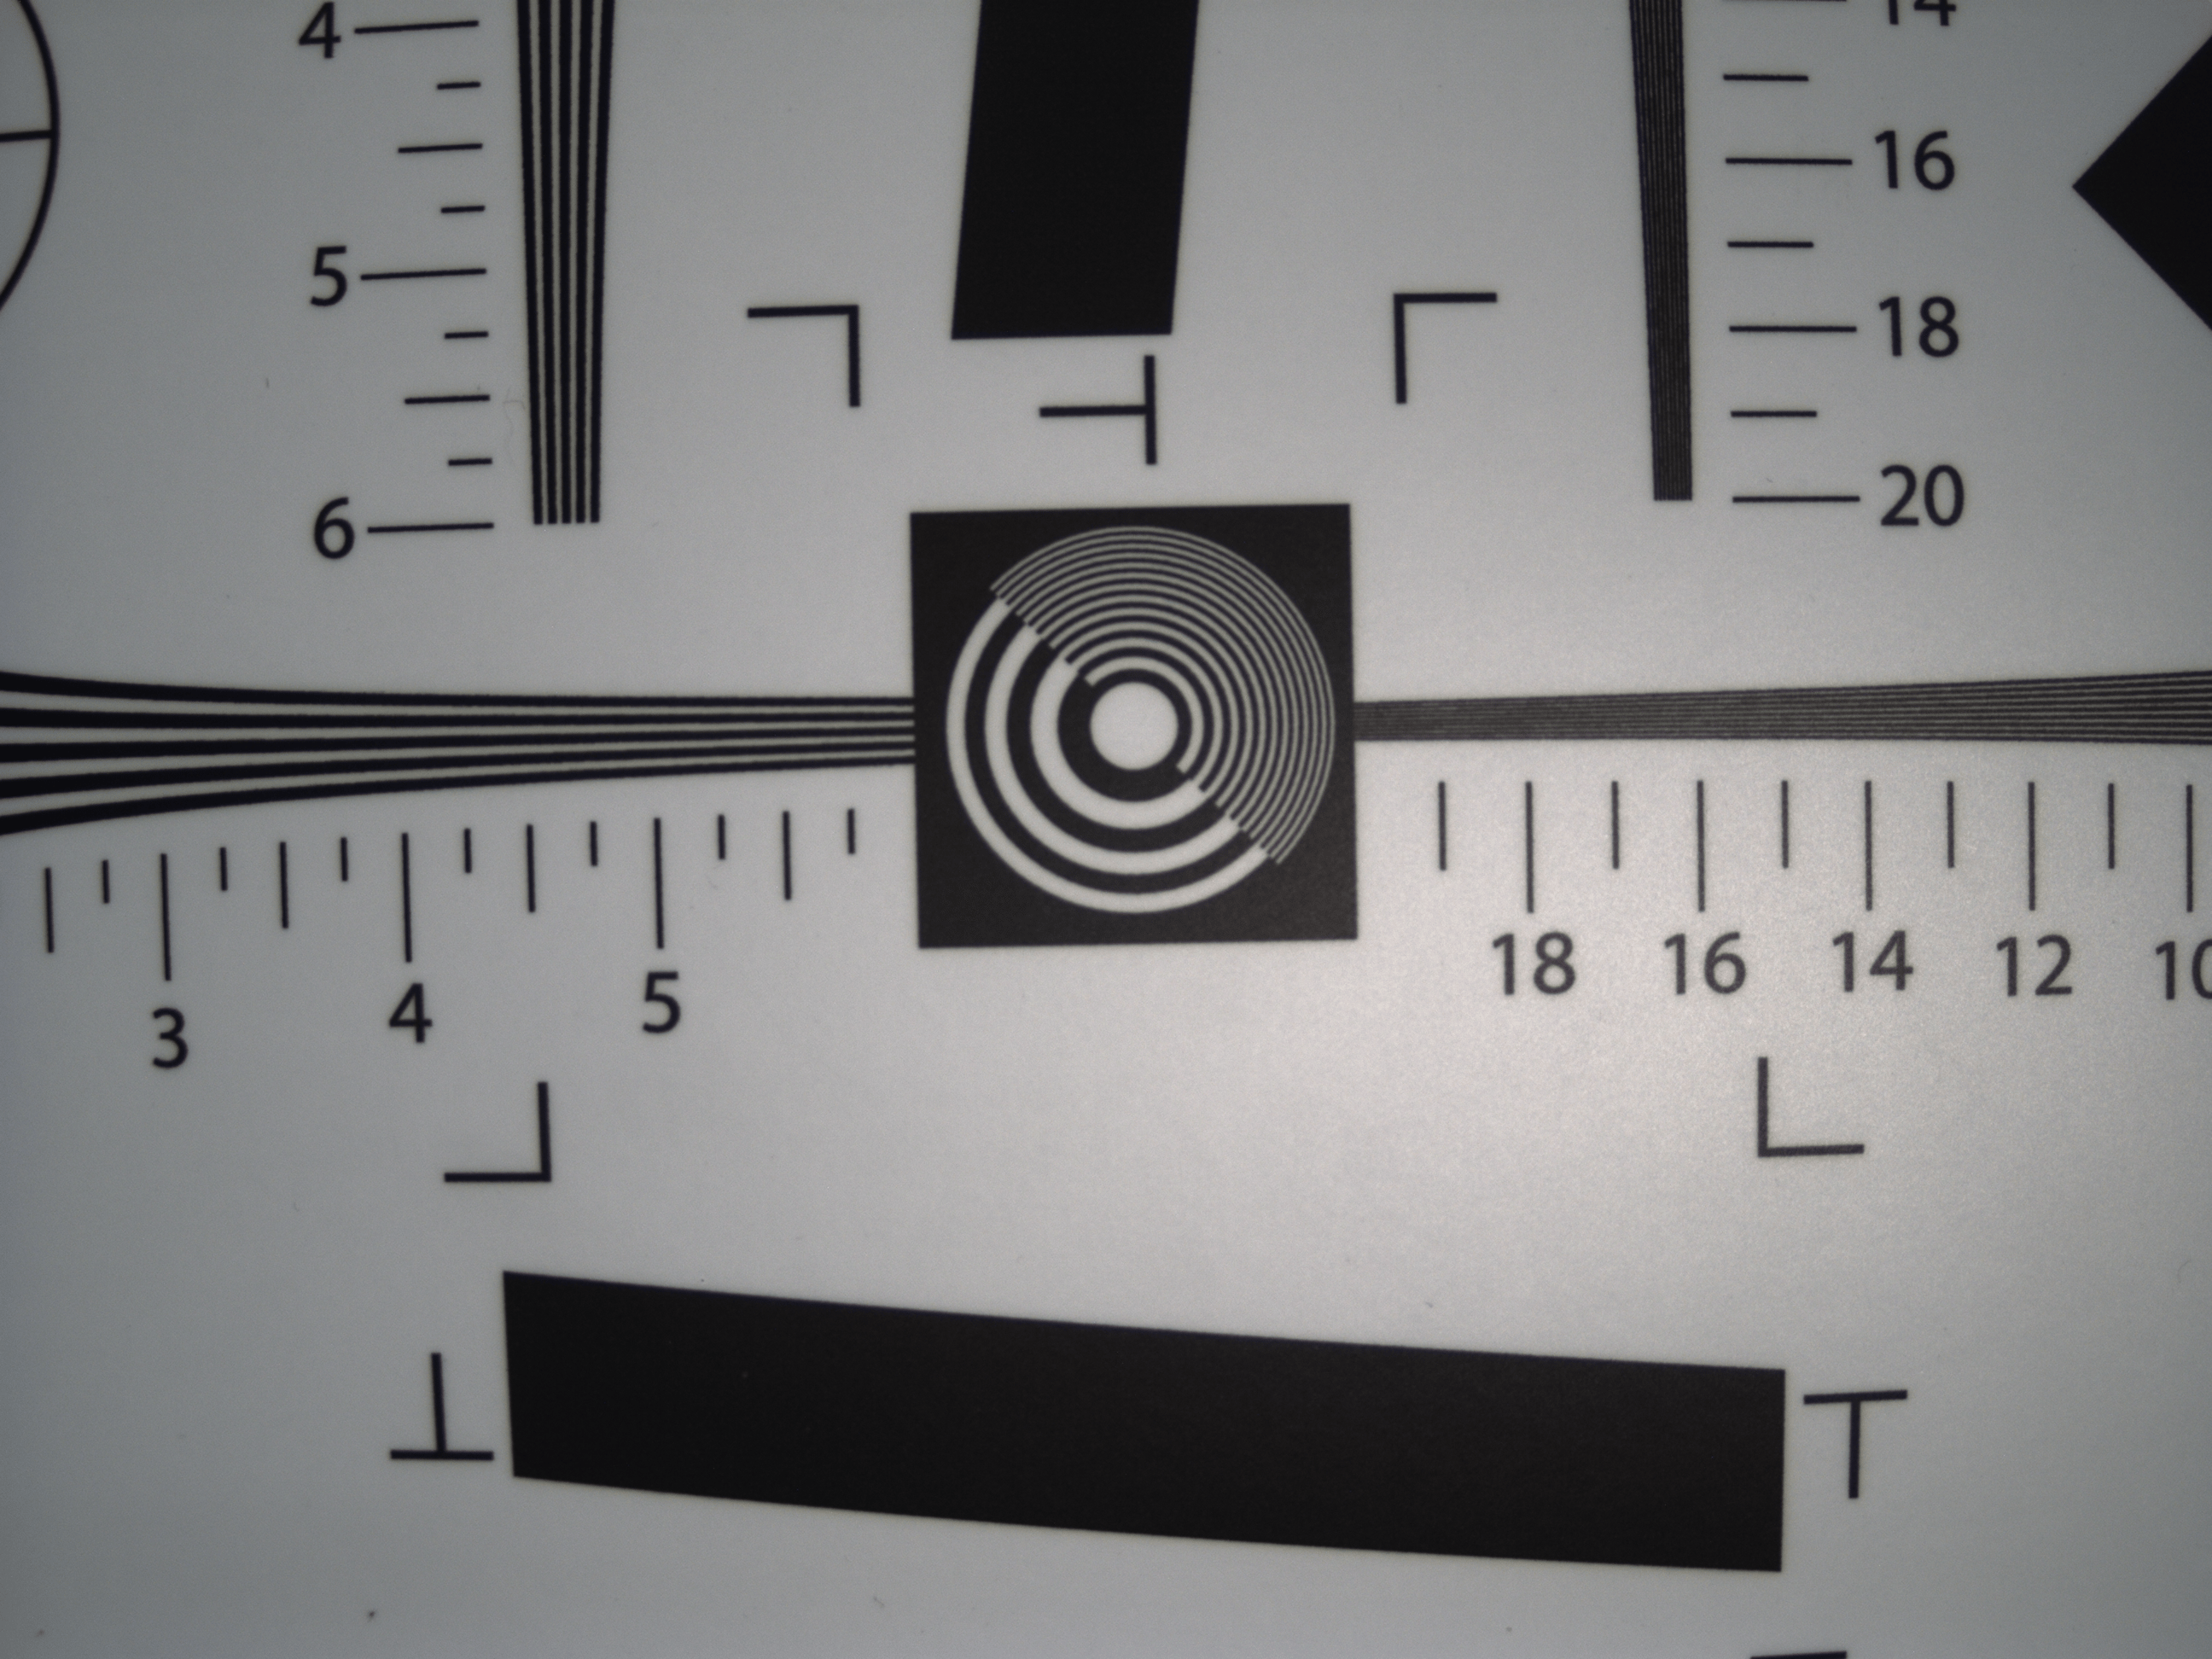
\includegraphics[width=.22\linewidth]{Figures/C4/FOV/VIS/V/30_3.png} \\
         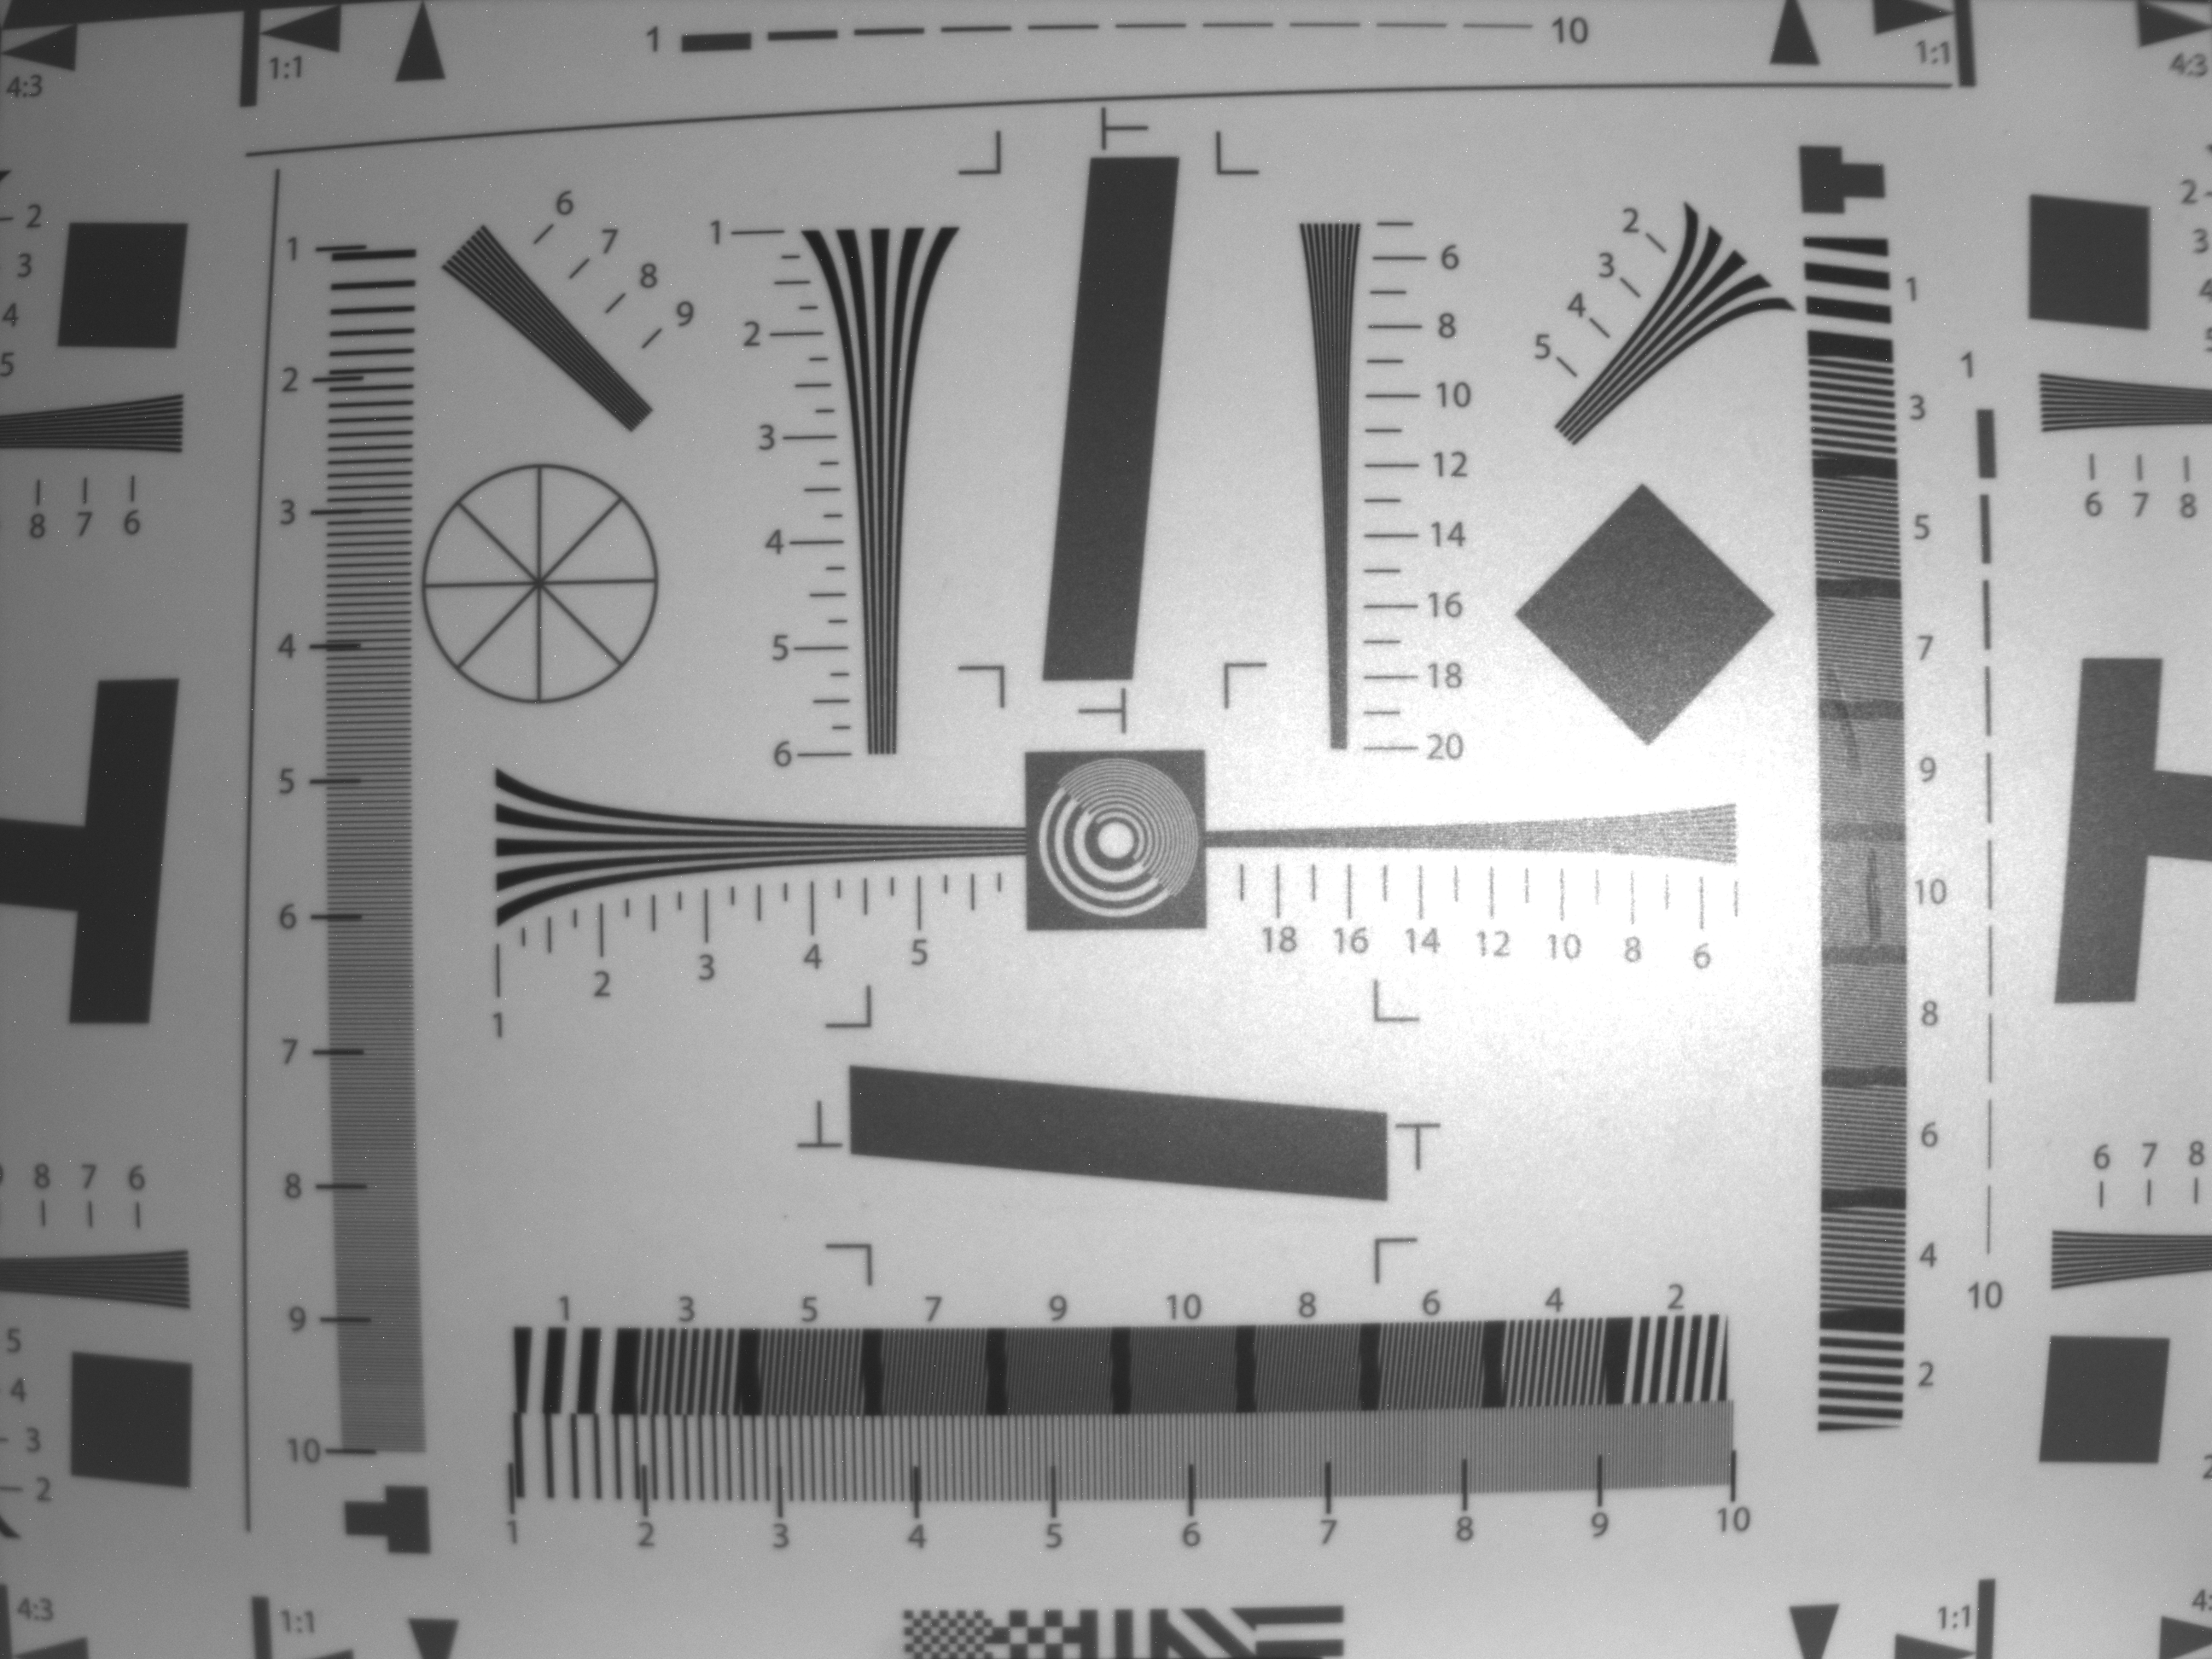
\includegraphics[width=.22\linewidth]{Figures/C4/FOV/NIR/H/63.png} &
         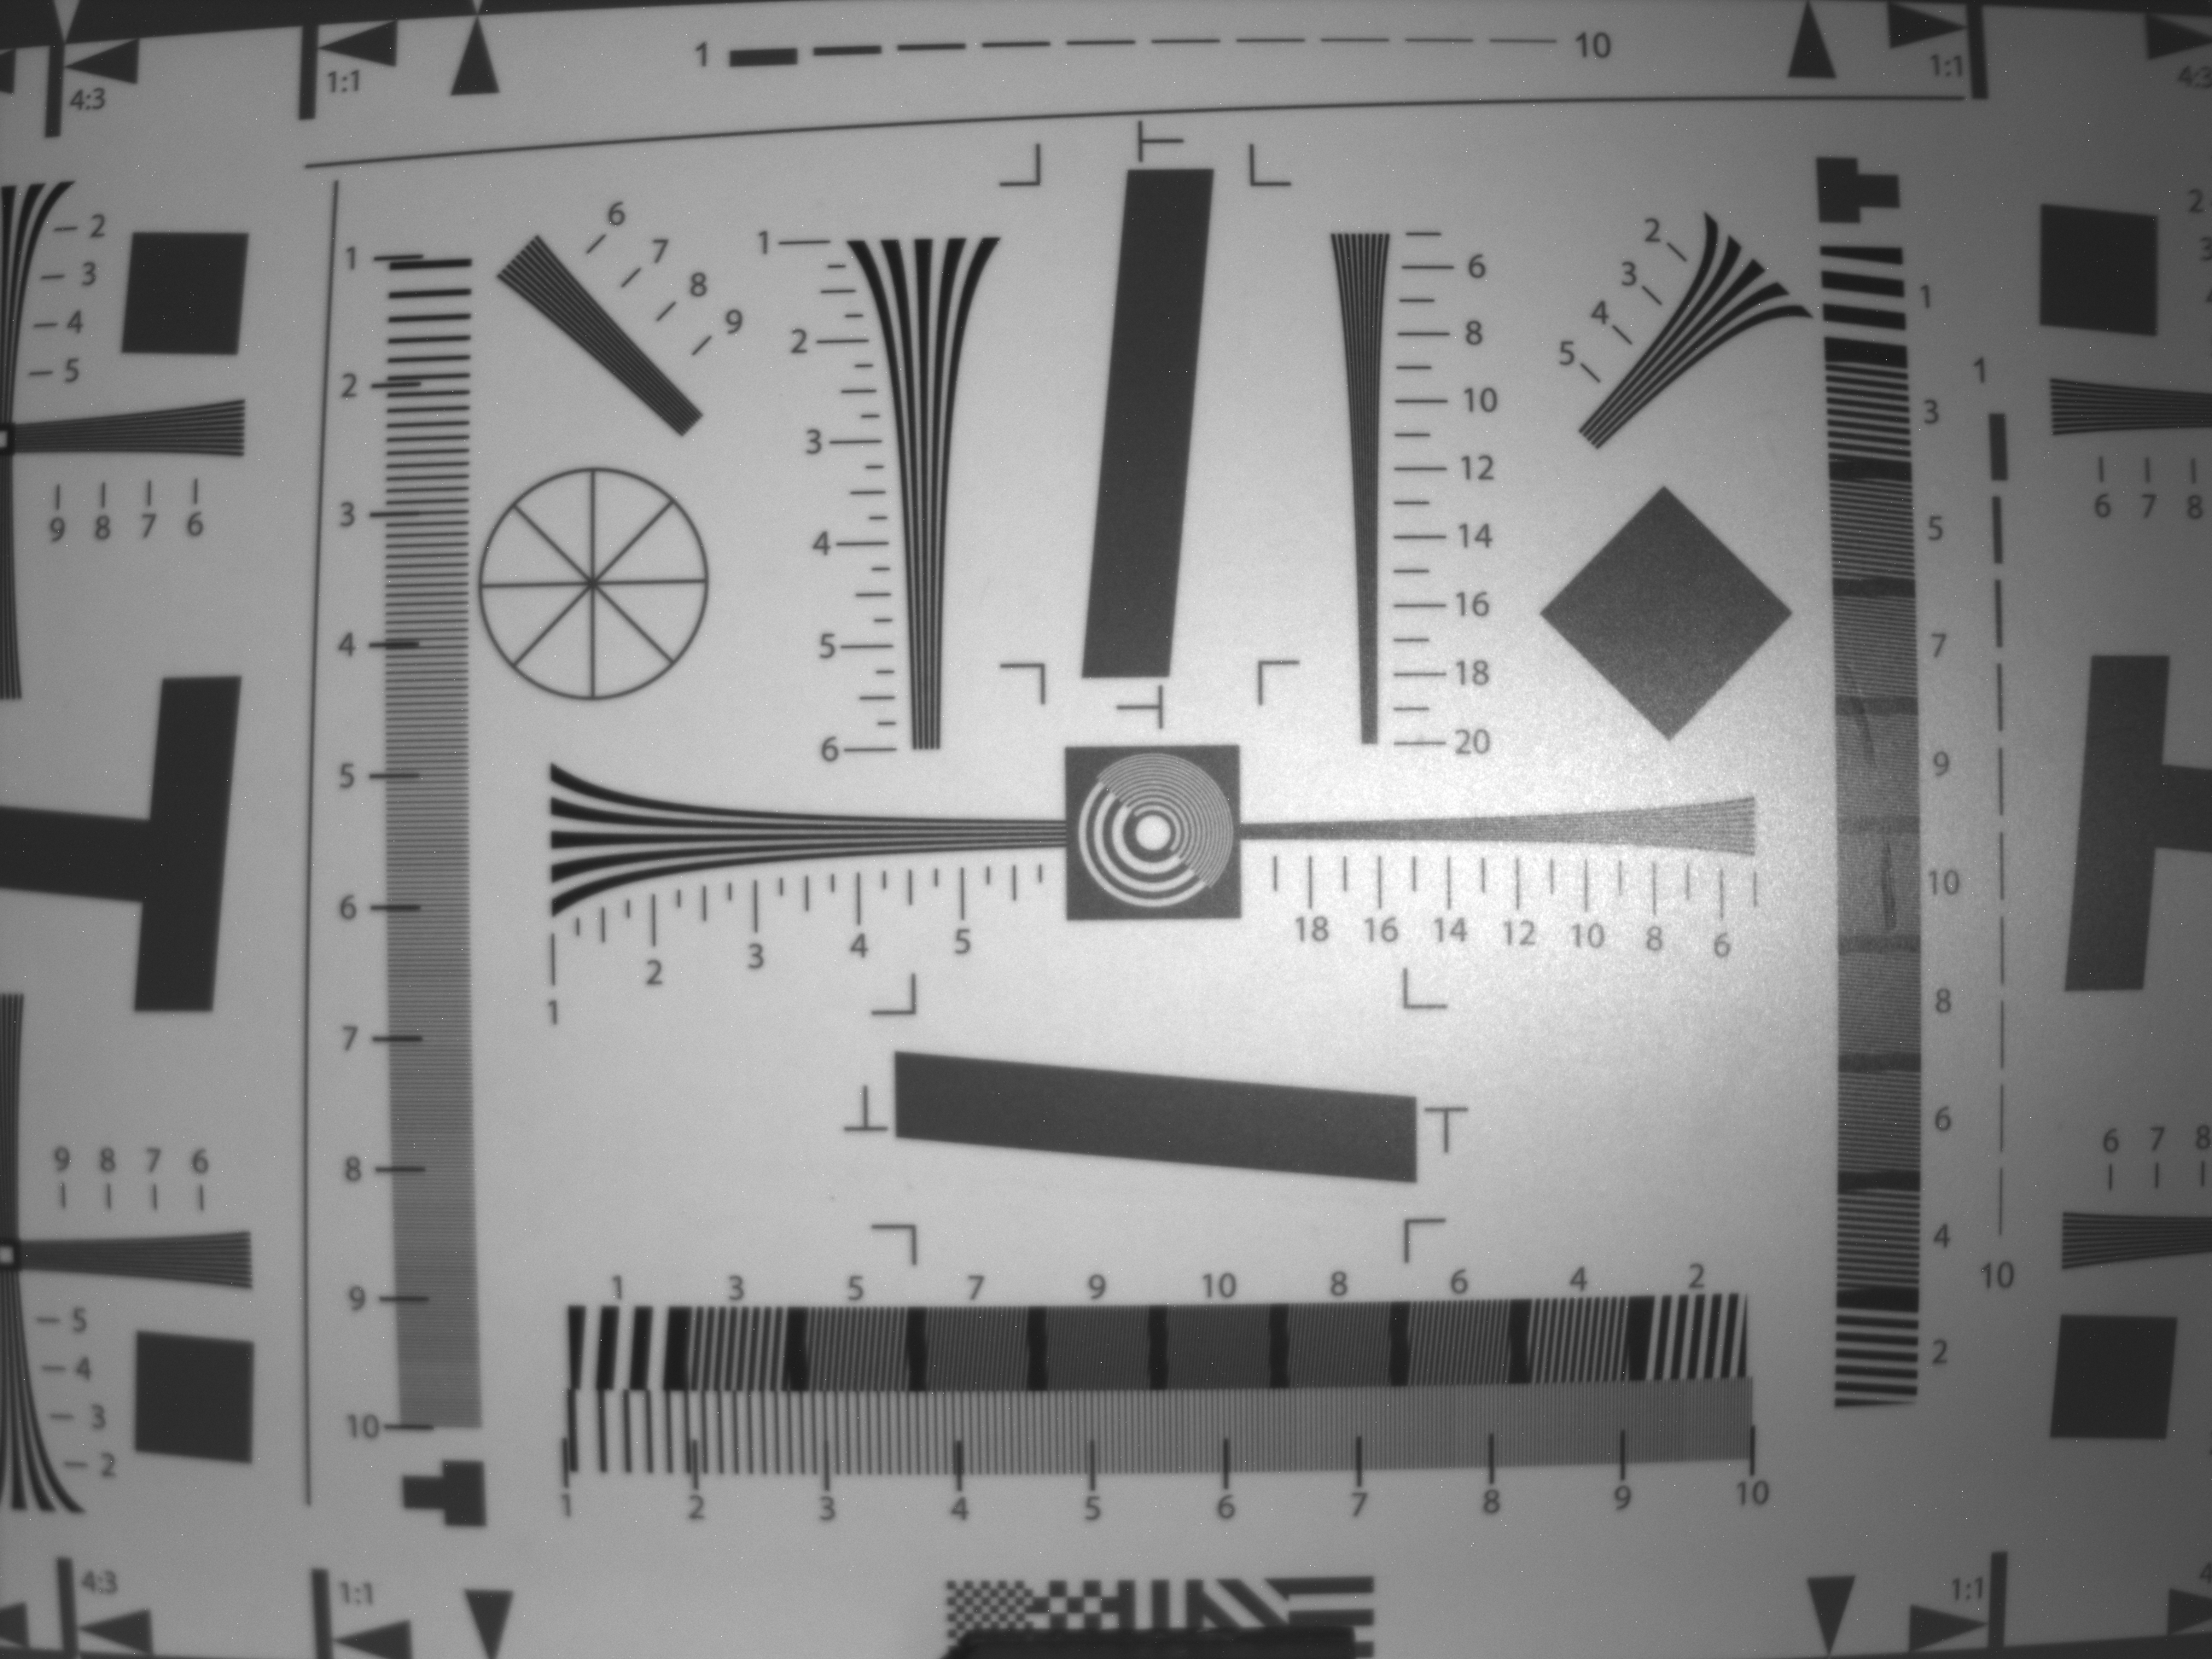
\includegraphics[width=.22\linewidth]{Figures/C4/FOV/NIR/V/65.png} &
         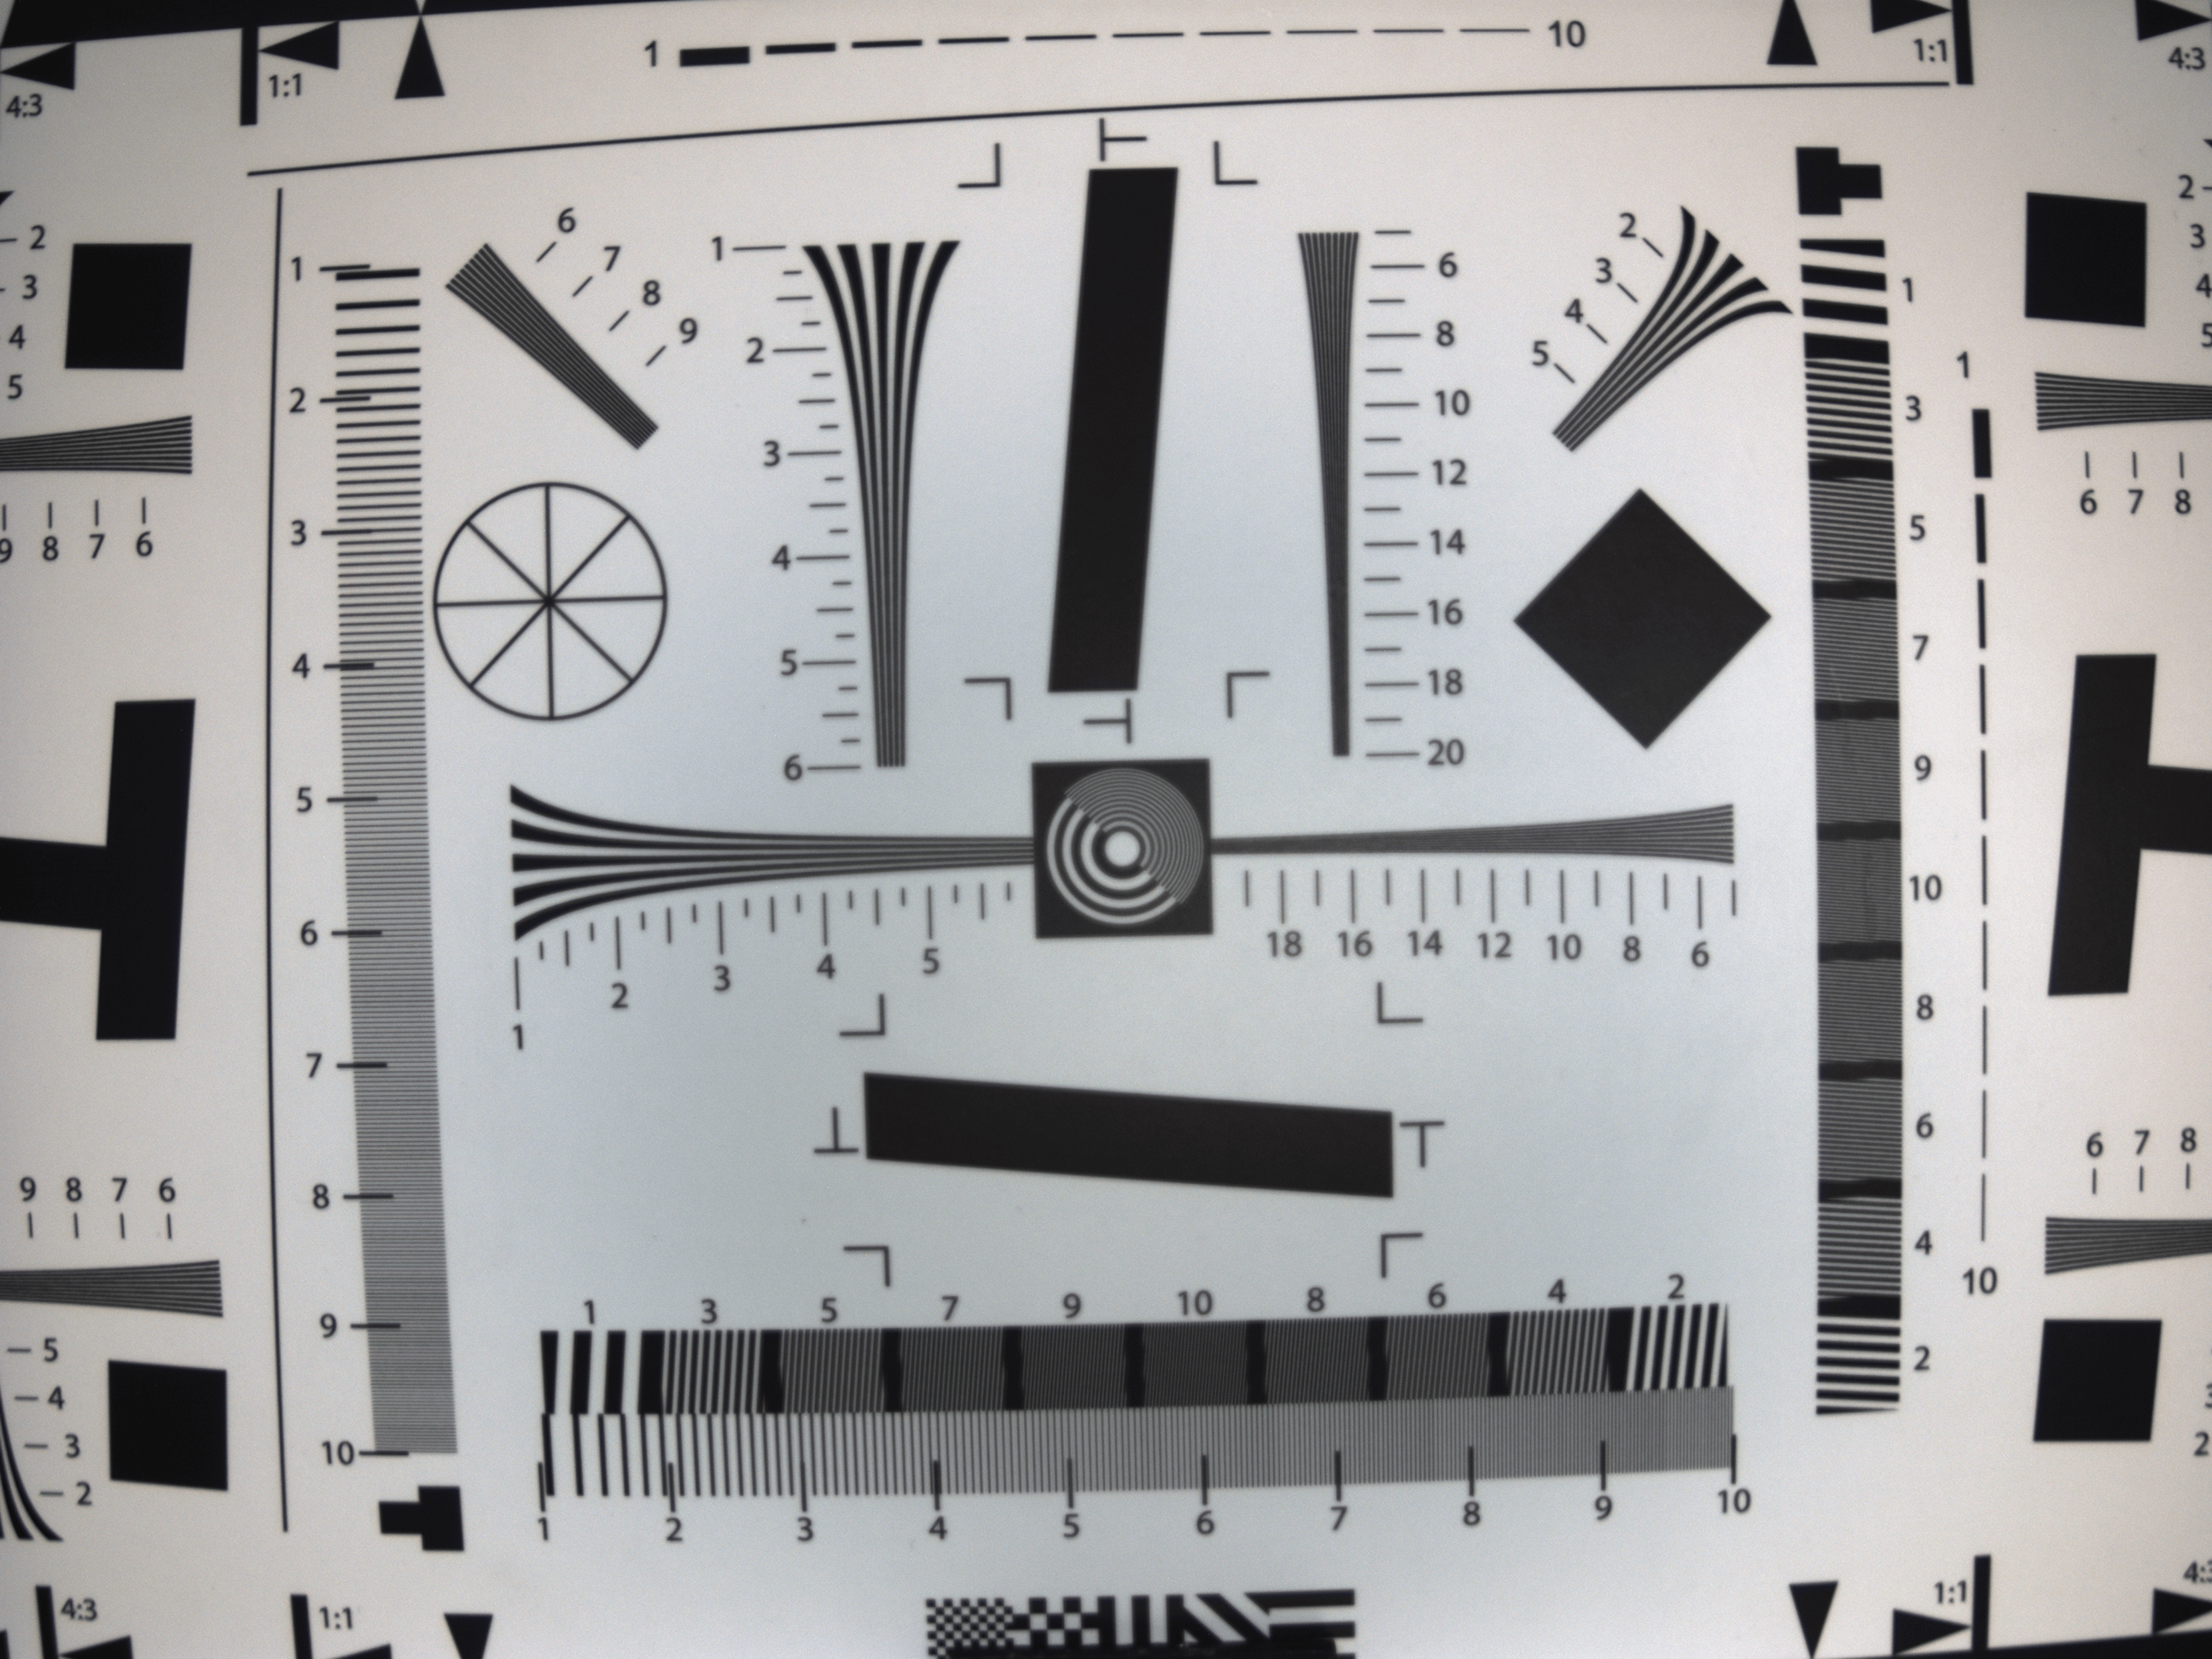
\includegraphics[width=.22\linewidth]{Figures/C4/FOV/VIS/H/69_4.png} &
         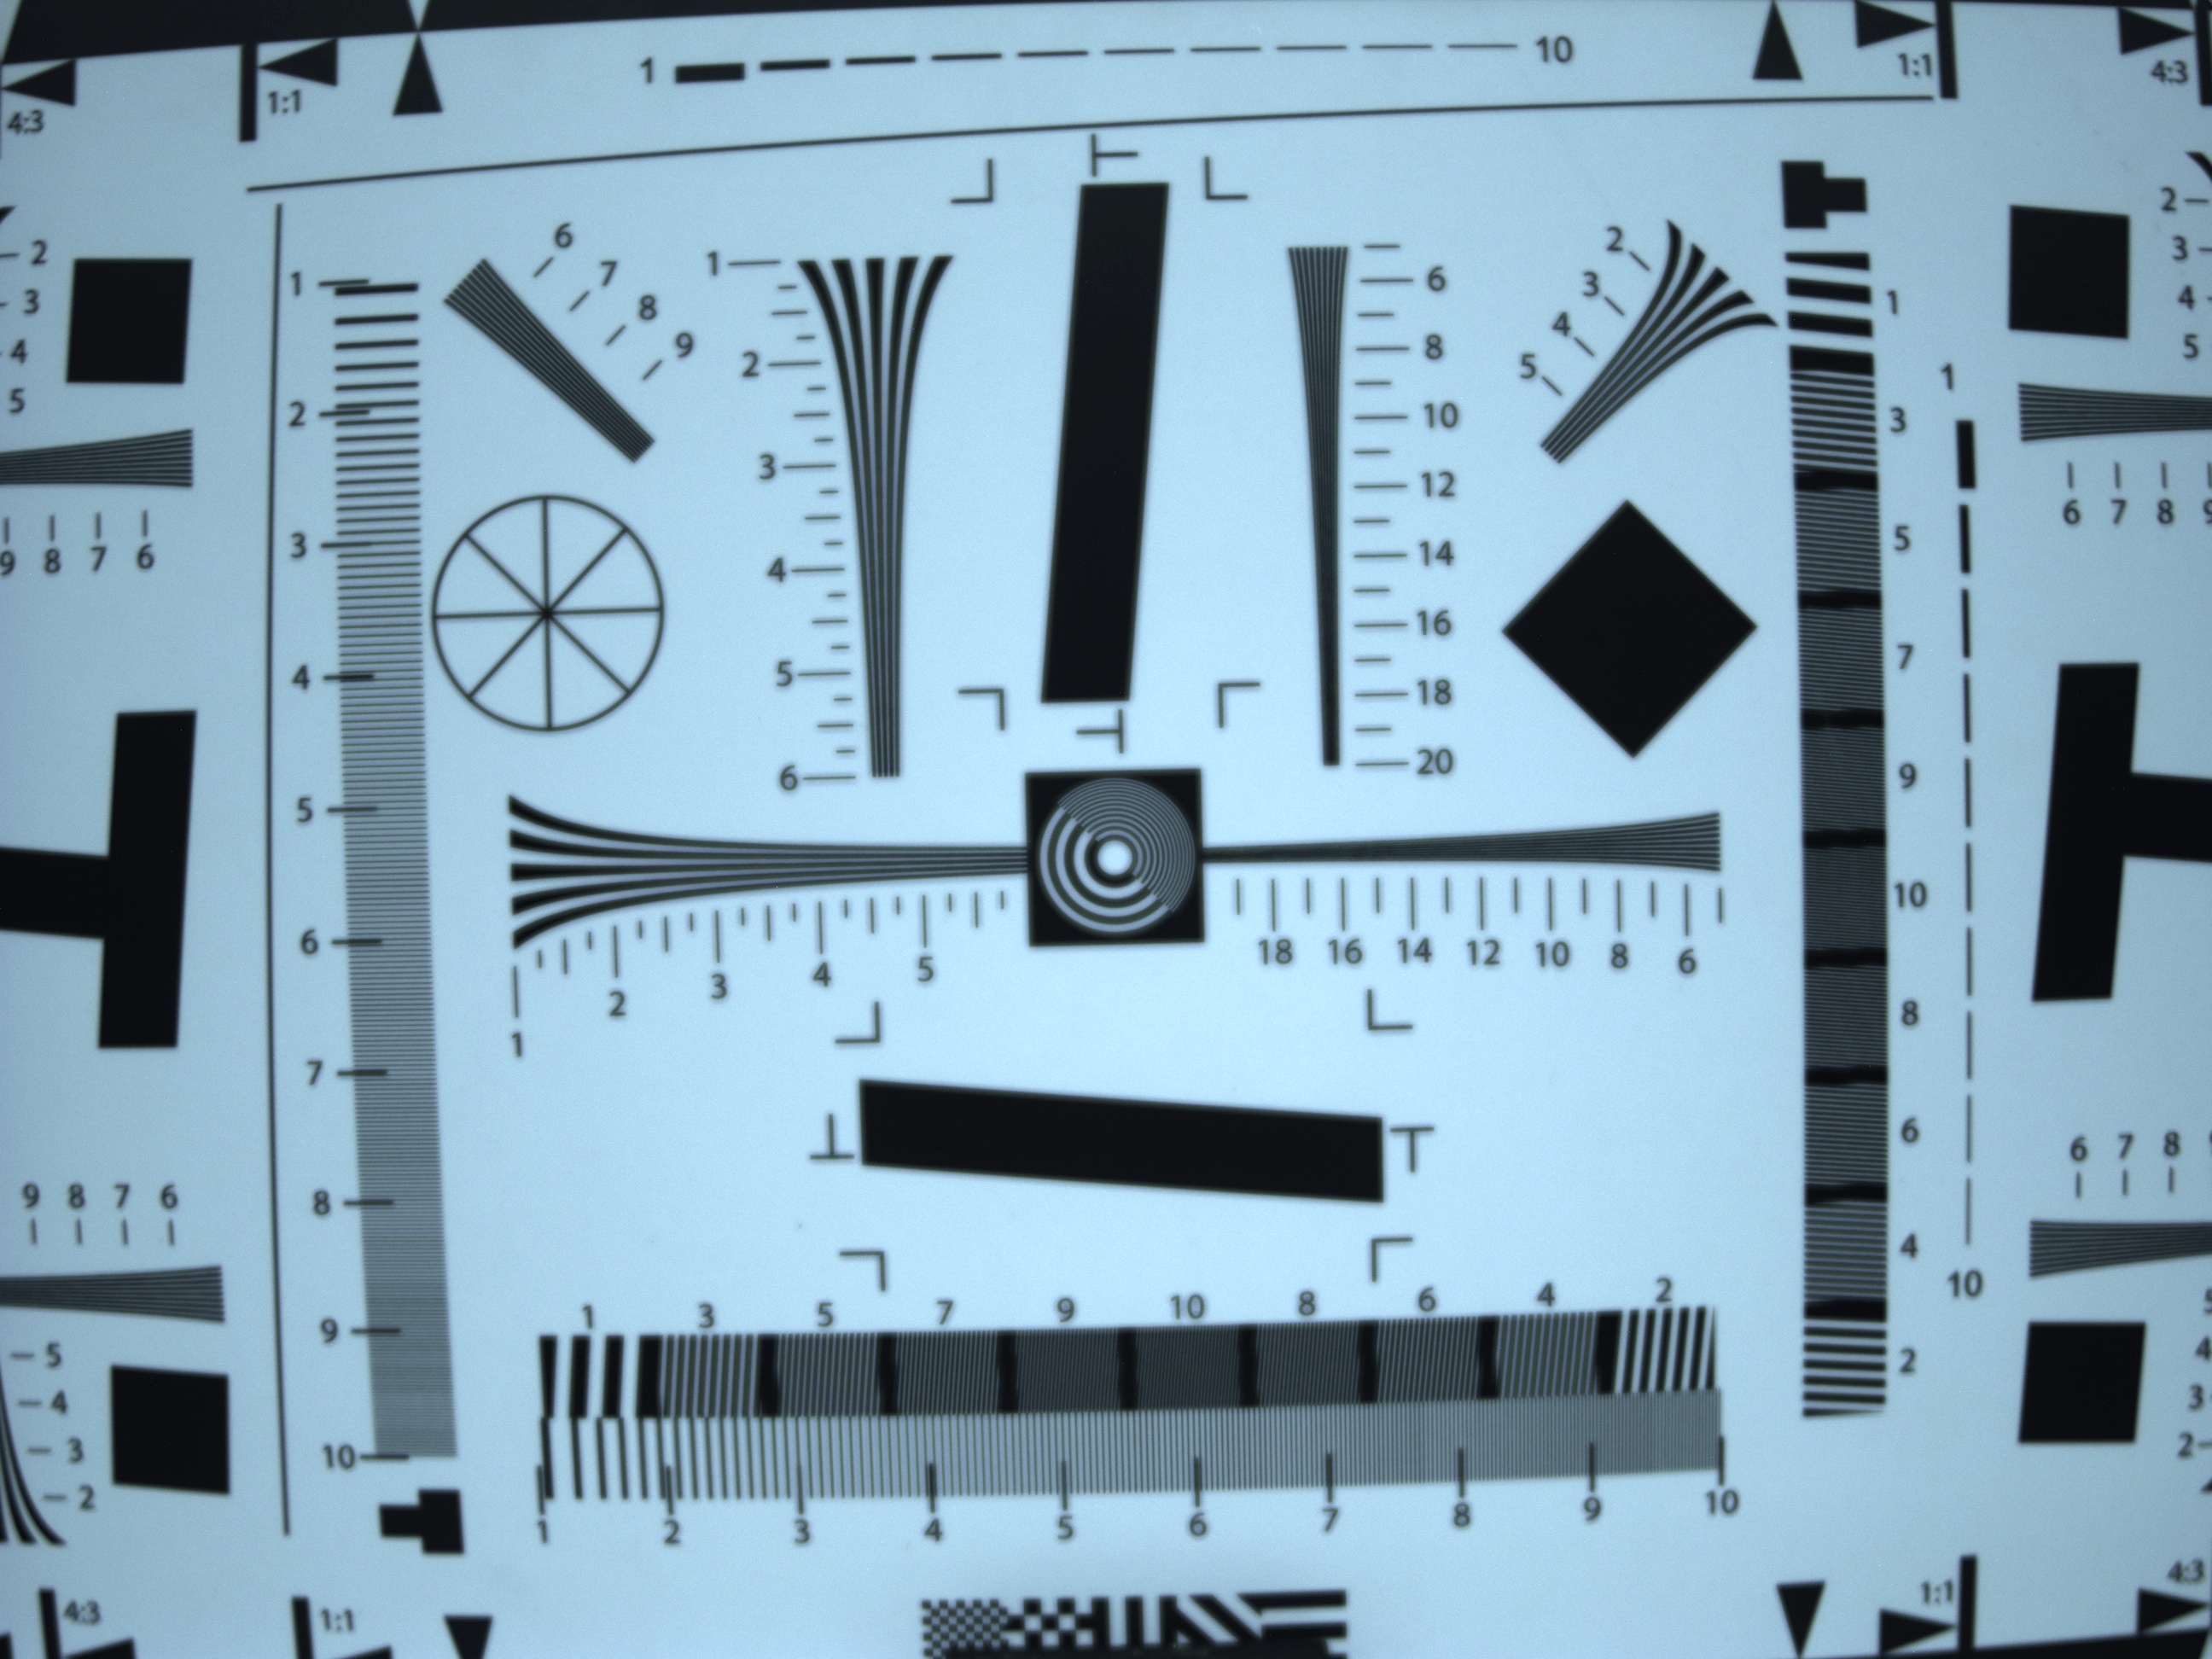
\includegraphics[width=.22\linewidth]{Figures/C4/FOV/VIS/V/70.png} \\
       \end{tabular}
       \caption{Imágenes originales para la medición del FOV horizontal (H)
                y vertical (V) en tres distancias de trabajo.}
       \label{fig:fov_montage}
     \end{figure}
     
     Las mediciones, convertidas a metros, se resumen en la Tabla \ref{tab:fov_raw_wd}, donde cada FOV se acompaña de una incertidumbre instrumental \(\sigma=1\) mm.
     
     % \begin{table}[H]
     %   \centering
     %   \caption{WD y FOV medidos para cada sistema óptico y orientación}
     %   \label{tab:fov_raw_wd}
     %   \small
     %   \setlength{\tabcolsep}{4pt} % Espaciado más compacto entre columnas
     %   \renewcommand{\arraystretch}{1.2} % Espaciado entre filas
     %   \begin{tabularx}{\textwidth}{|c|>{\centering\arraybackslash}X
     %                                     >{\centering\arraybackslash}X
     %                                     >{\centering\arraybackslash}X
     %                                     >{\centering\arraybackslash}X|
     %                                     >{\centering\arraybackslash}X
     %                                     >{\centering\arraybackslash}X
     %                                     >{\centering\arraybackslash}X
     %                                     >{\centering\arraybackslash}X|}
     %     \hline
     %     \rowcolor[HTML]{EFEFEF}
     %     & \multicolumn{4}{c|}{\textbf{NIR (Sis.~6)}} 
     %     & \multicolumn{4}{c|}{\textbf{VIS (Sis.~7)}} \\ \cline{2-9}
     %     \rowcolor[HTML]{EFEFEF}
     %     \textbf{Prueba} 
     %       & WD$_H$ [m] & FOV$_H$ [m] & WD$_V$ [m] & FOV$_V$ [m] 
     %       & WD$_H$ [m] & FOV$_H$ [m] & WD$_V$ [m] & FOV$_V$ [m] \\ 
     %     \hline
     %     1 & 0.071 & 0.0350 & 0.087 & 0.0350 & 0.092 & 0.0350 & 0.107 & 0.0350 \\
     %     2 & 0.331 & 0.231  & 0.350 & 0.180  & 0.379 & 0.239  & 0.303 & 0.138  \\
     %     3 & 0.650 & 0.468  & 0.650 & 0.349  & 0.694 & 0.458  & 0.700 & 0.342  \\ 
     %     \hline
     %   \end{tabularx}
     % \end{table}
 
     
     
     Aplicando regresión lineal ponderada (Deming) con pesos \(w=1/\sigma\), los ajustes óptimos fueron:
     
     \[
     \begin{aligned}
     \text{VIS:}\;&\mathrm{FOV_H}=(0.7025\pm0.0045)\,\mathrm{WD}-(0.0288\pm0.0021),\\
     \text{VIS:}\;&\mathrm{FOV_V}=(0.5171\pm0.0029)\,\mathrm{WD}-(0.0197\pm0.0013),\\
     \text{NIR:}\;&\mathrm{FOV_H}=(0.7477\pm0.0031)\,\mathrm{WD}-(0.0175\pm0.0013),\\
     \text{NIR:}\;&\mathrm{FOV_V}=(0.5579\pm0.0034)\,\mathrm{WD}-(0.0141\pm0.0015).
     \end{aligned}
     \]
     
     La Figura \ref{fig:fov_reg_combined} ilustra los ajustes con sus bandas de confianza \(1\sigma\).
     
     \begin{figure}[H]
     \centering
       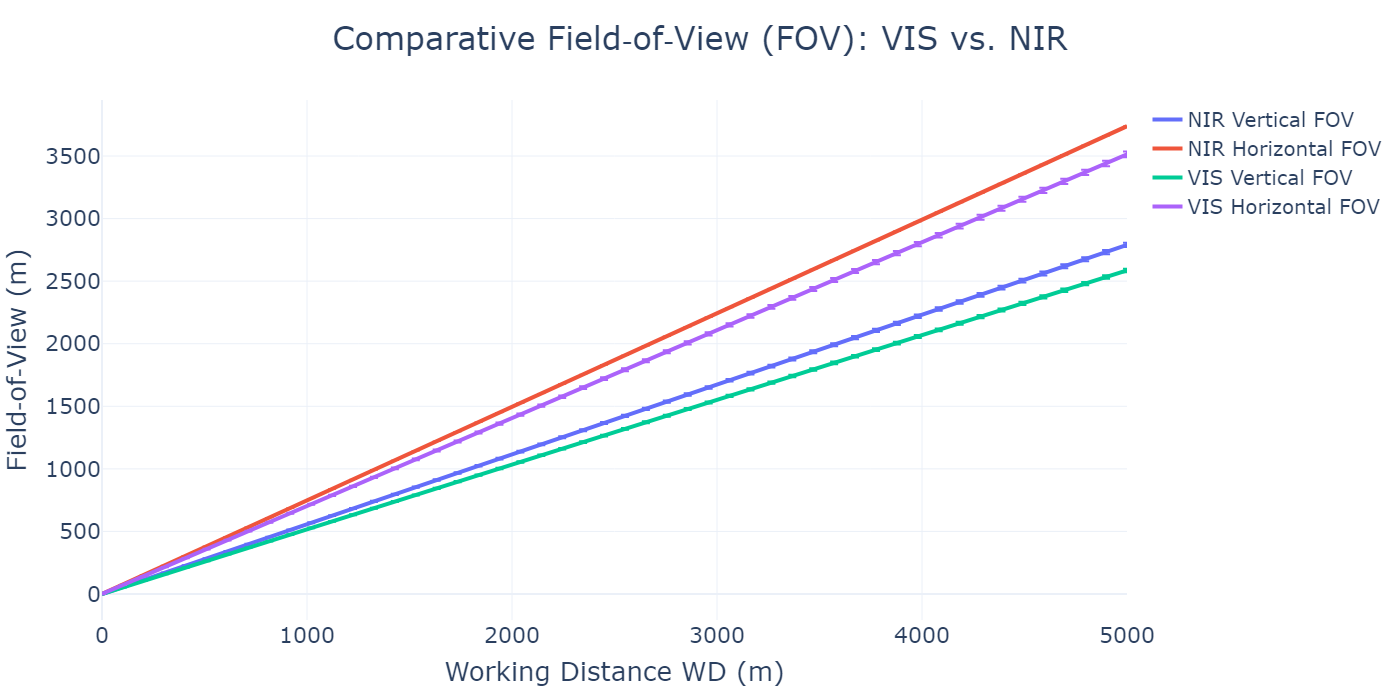
\includegraphics[width=1\linewidth]{Figures/C4/FOV.png}
       \caption{Ajuste lineal ponderado de FOV vs.\ WD para los cuatro casos: VIS–H, VIS–V, NIR–H y NIR–V .}
       \label{fig:fov_reg_combined}
     \end{figure}
     
 
     
     La Tabla \ref{tab:fov_pred_vs_theory_HV} compara el FOV horizontal predicho
     por los ajustes empíricos con los valores teóricos calculados en
     la Sección \ref{sec:cad_sim} para alturas de 50 m, 1000 m y 5000 m.
     
 
     
     % \begin{table}[H]
     %   \centering
     %   \caption{Comparativa empírico vs.\ teórico para FOV horizontal (H) y vertical (V).}
     %   \label{tab:fov_pred_vs_theory_HV}
     %   \small
     %   \begin{tabular*}{\columnwidth}{@{\extracolsep{\fill}}|
     %       c|
     %       rrrr|
     %       rrrr|
     %     }
     %     \toprule
     %      & \multicolumn{4}{c|}{\shortstack{\textbf{VIS}\\(Sis.~7)}} 
     %        & \multicolumn{4}{c|}{\shortstack{\textbf{NIR}\\(Sis.~6)}} \\
     %     \midrule
     %     \textbf{Altura}
     %       & \shortstack{Pred H\\[m]} 
     %       & \shortstack{Teo H\\[m]} 
     %       & \shortstack{Pred V\\[m]} 
     %       & \shortstack{Teo V\\[m]} 
     %       & \shortstack{Pred H\\[m]} 
     %       & \shortstack{Teo H\\[m]} 
     %       & \shortstack{Pred V\\[m]} 
     %       & \shortstack{Teo V\\[m]} \\
     %     \midrule
     %     50\,m   
     %       &  35.10  &  25.16   &  25.84  &  18.87  
     %       &  37.37  &  26.73   &  27.88  &  20.05  \\
     %     1000\,m 
     %       & 702.50  & 503.20   & 517.08  & 377.40  
     %       & 747.70  & 534.60   & 557.90  & 400.95  \\
     %     5000\,m 
     %       & 3512.00 & 2516.00  & 2585.48 & 1887.00 
     %       & 3737.00 & 2673.00  & 2788.89 & 2004.75 \\
     %     \bottomrule
     %   \end{tabular*}
     % \end{table}
 
     
 
     Con estos resultados, se puedes definir las discrepancias como:
     \[
       \Delta_{\mathrm{abs}} = FOV_{\mathrm{pred}} - FOV_{\mathrm{teo}},
       \qquad
       \Delta_{\mathrm{rel}} = \frac{\Delta_{\mathrm{abs}}}{FOV_{\mathrm{teo}}}\times100\%.
     \]
     A continuación se presentan los resultados para cada altura y sistema:
     
     \begin{align*}
     50\,\mathrm{m}:&\quad
     \Delta_{\mathrm{abs}}^{\mathrm{VIS}} = 35.10 - 33.54 = 1.56\,\mathrm{m}, 
     \quad
     \Delta_{\mathrm{rel}}^{\mathrm{VIS}} = \frac{1.56}{33.54}\times100\%\approx4.65\%,\\
     &\quad
     \Delta_{\mathrm{abs}}^{\mathrm{NIR}} = 37.37 - 35.64 = 1.73\,\mathrm{m}, 
     \quad
     \Delta_{\mathrm{rel}}^{\mathrm{NIR}} = \frac{1.73}{35.64}\times100\%\approx4.85\%.\\[6pt]
     1000\,\mathrm{m}:&\quad
     \Delta_{\mathrm{abs}}^{\mathrm{VIS}} = 702.5 - 670.9 = 31.6\,\mathrm{m}, 
     \quad
     \Delta_{\mathrm{rel}}^{\mathrm{VIS}} = \frac{31.6}{670.9}\times100\%\approx4.71\%,\\
     &\quad
     \Delta_{\mathrm{abs}}^{\mathrm{NIR}} = 747.7 - 712.8 = 34.9\,\mathrm{m}, 
     \quad
     \Delta_{\mathrm{rel}}^{\mathrm{NIR}} = \frac{34.9}{712.8}\times100\%\approx4.90\%.\\[6pt]
     5000\,\mathrm{m}:&\quad
     \Delta_{\mathrm{abs}}^{\mathrm{VIS}} = 3512 - 3354 = 158\,\mathrm{m}, 
     \quad
     \Delta_{\mathrm{rel}}^{\mathrm{VIS}} = \frac{158}{3354}\times100\%\approx4.71\%,\\
     &\quad
     \Delta_{\mathrm{abs}}^{\mathrm{NIR}} = 3737 - 3564 = 173\,\mathrm{m}, 
     \quad
     \Delta_{\mathrm{rel}}^{\mathrm{NIR}} = \frac{173}{3564}\times100\%\approx4.86\%.
     \end{align*}
 
     
     Los resultados confirman que, en ambos sistemas, la discrepancia relativa se mantiene entre un 4.6–4.9 \% independientemente de la altura de operación. Este sesgo prácticamente constante refuerza la hipótesis de un error geométrico sistemático (distorsión radial y paralaje en la medida de WD) que debe corregirse antes de la generación de ortomosaicos. 
     
     
     \subsection{Caracterización angular: AFOV vs.\ WD}
     Las figuras \ref{fig:afov} presentan dos curvas para cada sistema: horizontal y vertical. En el caso VIS, el AFOV crece hacia el valor teórico sin sobrepasarlo; en NIR, el experimento supera ligeramente el teórico a medida que WD aumenta, sugiriendo un enfoque ligeramente desajustado. \\
 
     1\begin{figure}[H]
       \centering
       \begin{subfigure}[b]{.9\linewidth}
         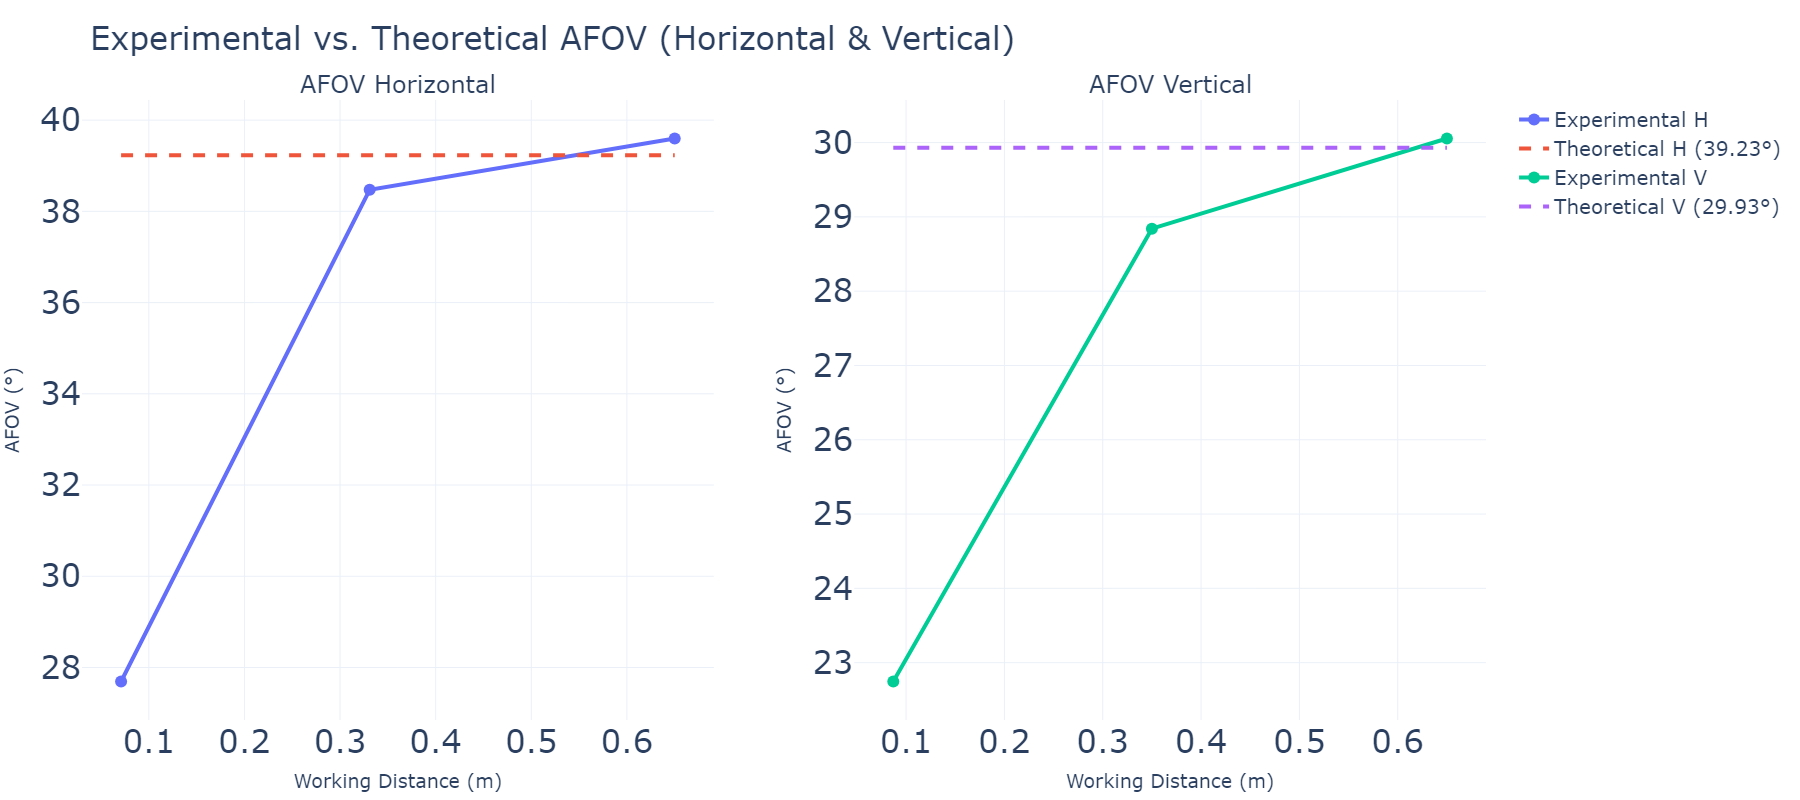
\includegraphics[width=\linewidth]{Figures/C4/afov_nir.png}
         \caption{NIR – Sistema 6}
       \end{subfigure}
       \hfill
       \begin{subfigure}[b]{0.9\linewidth}
         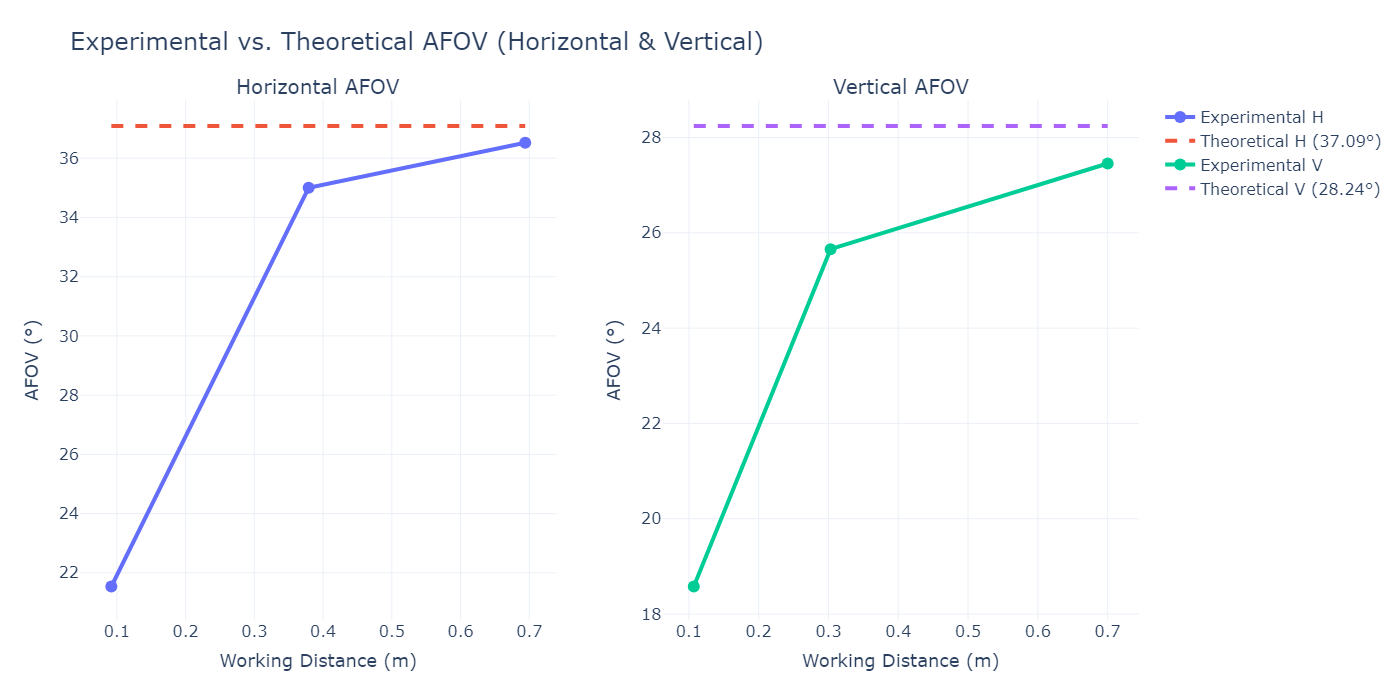
\includegraphics[width=\linewidth]{Figures/C4/afov_vis.png}
         \caption{VIS – Sistema 7}
       \end{subfigure}
       \caption{AFOV experimental vs.\ WD (flecha punteada: valor teórico).}
       \label{fig:afov}
     \end{figure}
     
     Para cuantificar la convergencia, en la Tabla~\ref{tab:afov_exp} se resumen los valores experimentales de AFOV en los tres WD medidos. A la mayor distancia, la discrepancia horizontal con el valor teórico ($37.1^\circ$ para VIS y $39.3^\circ$ para NIR) es:
     \[
     \begin{aligned}
     \Delta_{\rm abs}^{\rm VIS\text{-}H} &=36.52^\circ - 37.10^\circ = -0.58^\circ\quad(\Delta_{\rm rel}\approx1.6\%),\\
     \Delta_{\rm abs}^{\rm NIR\text{-}H} &=39.60^\circ - 39.30^\circ = +0.30^\circ\quad(\Delta_{\rm rel}\approx0.8\%).
     \end{aligned}
     \]
     Verticalmente, comparando con el valor teórico de $28.24^\circ$, para WD máximo:
     \[
     \begin{aligned}
     \Delta_{\rm abs}^{\rm VIS\text{-}V} &=27.46^\circ - 28.24^\circ = -0.78^\circ\quad(\Delta_{\rm rel}\approx2.8\%),\\
     \Delta_{\rm abs}^{\rm NIR\text{-}V} &=30.05^\circ - 28.24^\circ = +1.81^\circ\quad(\Delta_{\rm rel}\approx6.4\%).
     \end{aligned}
     \]
     
     \begin{table}[H]
       \centering
       \caption{AFOV experimental para WD de 0.07–0.09 m, 0.30–0.38 m y 0.65–0.70 m.}
       \label{tab:afov_exp}
       \begin{tabular}{lccc}
         \toprule
         Sistema & WD [m] & AFOV$_H$ [°] & AFOV$_V$ [°] \\
         \midrule
         \textbf{VIS (Sistema 7)} 
           & 0.09 & 21.54 & 18.58 \\
           & 0.38 & 35.00 & 25.66 \\
           & 0.69 & 36.52 & 27.46 \\
         \midrule
         \textbf{NIR (Sistema 6)} 
           & 0.07 & 27.69 & 22.75 \\
           & 0.33 & 38.47 & 28.84 \\
           & 0.65 & 39.60 & 30.05 \\
         \bottomrule
       \end{tabular}
     \end{table}
    
     \subsection{Modulation Transfer Function (MTF) Measurements}
      \label{sec:mtf_results}
      Aunque el montaje experimental para la caracterización de la MTF se describió en la metodología (véase la Figura~\ref{fig:srf_motaje}), durante las primeras pruebas se constató que el contraste entre las zonas claras y oscuras resultaba insuficiente para aplicar con fiabilidad el método ISO 12233. Según este estándar, el test chart debe presentar un contraste mínimo de 4:1 y una distribución de irradiancia lo más uniforme posible en ambas regiones, de modo que el histograma de intensidad exhiba dos picos nítidos (uno correspondiente a las zonas claras y otro a las zonas oscuras). Sin embargo, al analizar la carta de prueba impresa en papel mate —una reprografía de bajo costo— se observó una continuidad de valores intermedios y múltiples picos espurios que comprometían la extracción precisa de la Edge Spread Function (ESF). Esta carta de ruebas puede ser adquirida por proveedores de isntrumentos ópticos, pero su costo es elevado.\\

      \begin{figure}[h]
          \centering
          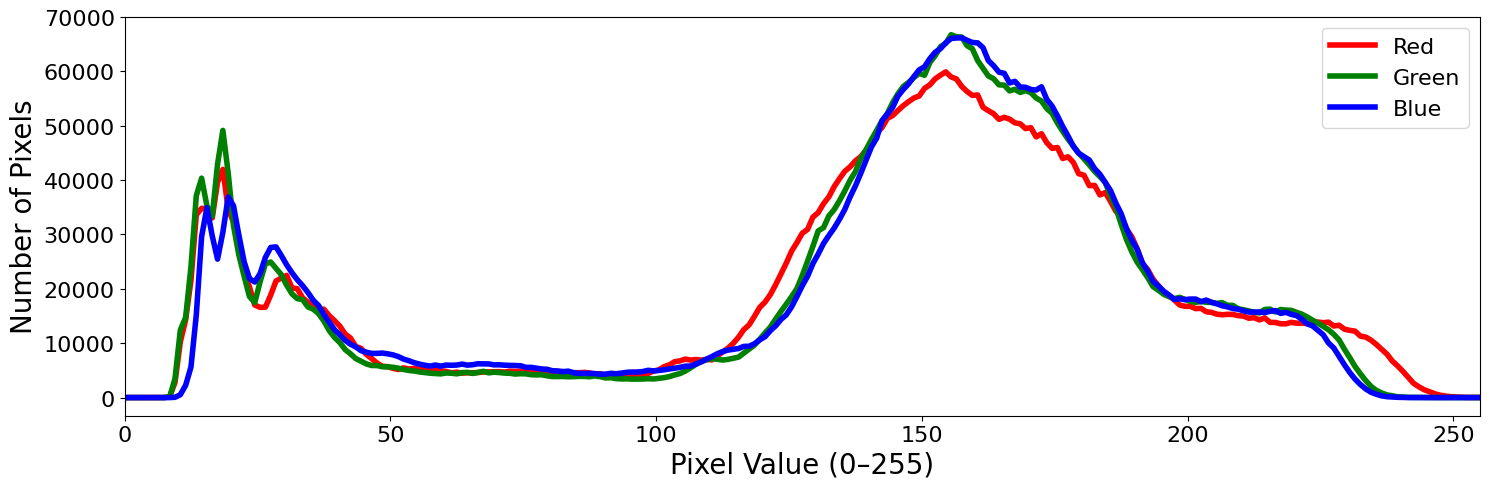
\includegraphics[width=0.7\linewidth]{Figures/C4/MTF_chart_hist.png}
          \caption{Histograma de la carta de prueba ISO 12233 impresa en papel mate. Se aprecian tres picos en la región oscura y dos picos muy anchos en la región clara, reflejo de una alta desviación estándar y de un contraste inferior al requerido por la norma.}
          \label{fig:histogram_iso12233}
      \end{figure}
      
      El origen de esta dispersión radica en dos factores principales. Primero, la calidad de impresión (impreso en una impresora de un proveedor local no especializado en cartas para pruebas ópticas de laboratorio) del test chart no garantizaba bordes suficientemente definidos ni un nvel de negros que proporsionaran el suficiente contraste. Segundo, el esquema de iluminación no siguió estrictamente la recomendación de emplear dos fuentes homogéneas (véase la Figura~\ref{fig:srf_motaje}), lo cual impidió alcanzar una irradiancia uniforme sobre la carta y acentuó las zonas de sombra y reflejo. Ante ello, se optó por un patrón de prueba empírico, el cual consistía en una hoja de papel inlcinada y un fondo oscuro, y por limitar la región de interés a un área de 104 $\times$ 104 píxeles, de forma que la iluminación pudiera controlarse de manera más rigurosa.\\
      
      La imagen finalmente utilizada para la determinación de la MTF —etiquetada como Figura~\ref{fig:enfoque}— fue corregida previamente, en primer lugar, de la corriente oscura según se describe en la Sección~\ref{subsub:corriente_oscura_espectrometro}, y, en segundo lugar, de los errores aleatorios mediante el promediado de múltiples capturas (tal como se detalló en la metodología de MTF). Sobre estas imágenes corregidas se generaron histogramas de intensidad para cada sistema, a fin de verificar que ahora sí se obtenía una distribución bimodal aceptable.
      
      \begin{figure}[h]
          \centering
          \begin{subfigure}[b]{\linewidth}
              \centering
              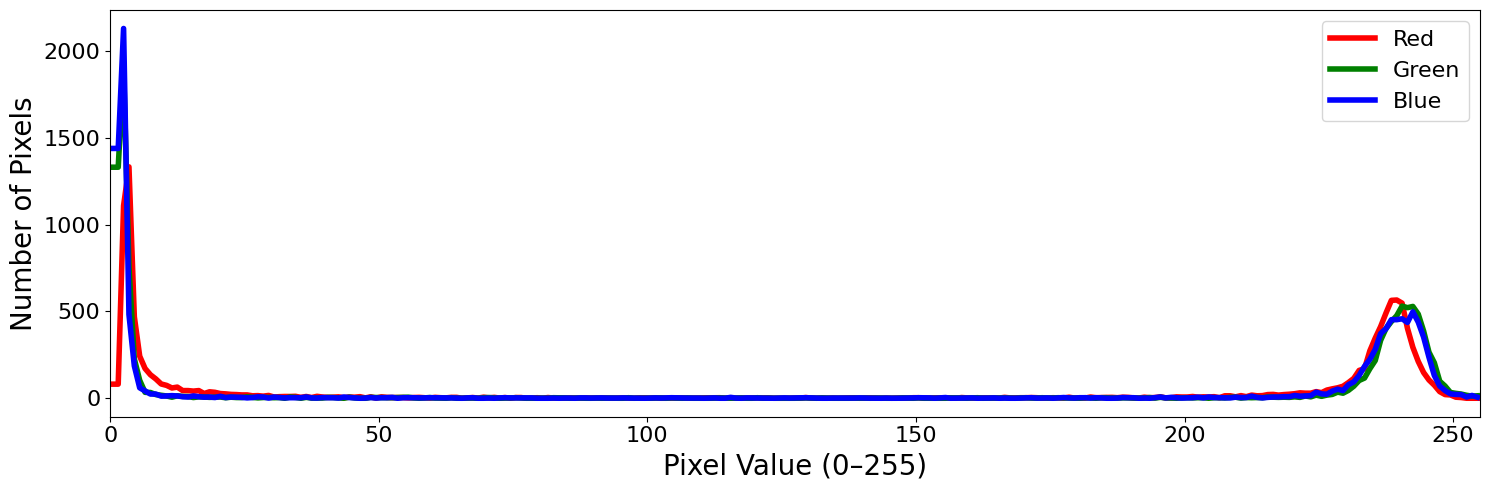
\includegraphics[width=\linewidth]{Figures/C4/hist_vis_MTF.png}
              \caption{Sistema VIS: histogramas de los canales R, G y B después de correcciones.}
              \label{fig:histogram_vis}
          \end{subfigure}
          \hfill
          \begin{subfigure}[b]{\linewidth}
              \centering
              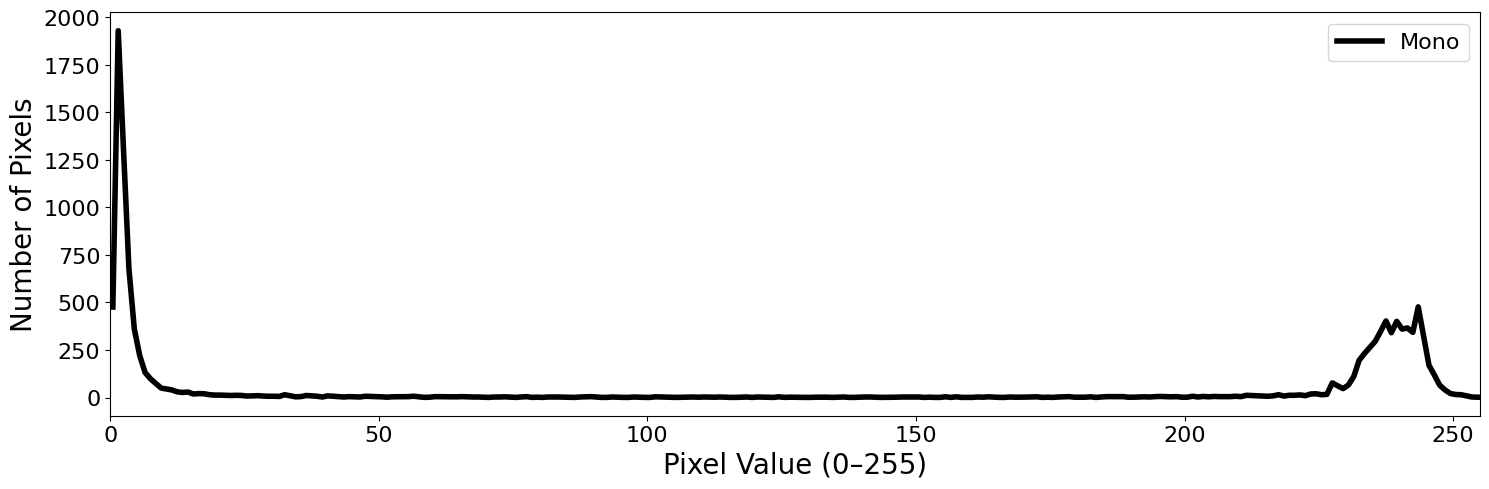
\includegraphics[width=\linewidth]{Figures/C4/hist_nir_MTF.png}
              \caption{Sistema NIR: histograma de su único canal tras correcciones.}
              \label{fig:histogram_nir}interés a un área de 104
          \end{subfigure}
          \caption{Distribución de valores de intensidad en imágenes corregidas (corriente oscura y ruido aleatorio) para los sistemas VIS y NIR, empleadas en la extracción de la MTF.}
          \label{fig:histogram_vis_nir}
      \end{figure}
      
      Con estas condiciones mejoradas se pudo proceder a extraer la ESF y, posteriormente, la Line Spread Function (LSF) y su transformada de Fourier para obtener las curvas de MTF de ambos sistemas. Este rigor en la corrección y control de iluminación garantiza que las mediciones resultantes reflejen fielmente la capacidad de resolución de los ópticos evaluados.      % Breve recordatorio de cómo se obtuvieron las curvas MTF (ISO 12233, número de imágenes, condiciones de enfoque, aperturas, exposición, etc.) 
      
    %---------------------------------------------------------------
    \subsubsection{MTF Curves for VIS and NIR Systems}
    \label{subsub:mtf_curves}
    %---------------------------------------------------------------
    Las curvas MTF se obtuvieron con el \textit{plugin} \texttt{SE\_MTF} de \textit{ImageJ} siguiendo el procedimiento descrito en la sección~\ref{sec:mtf_char}.  
    Para el sistema VIS (Sistema 7) se procesaron independientemente los tres canales \(R\), \(G\) y \(B\) y, adicionalmente, la imagen promedio (\textit{Mono}).  
    Para el sistema NIR (Sistema 6) únicamente se dispone de un canal monocromático.

    \begin{figure}[H]
        \centering
        %-----------------------------------------------------------
        \begin{subfigure}[b]{0.48\linewidth}
            \centering
            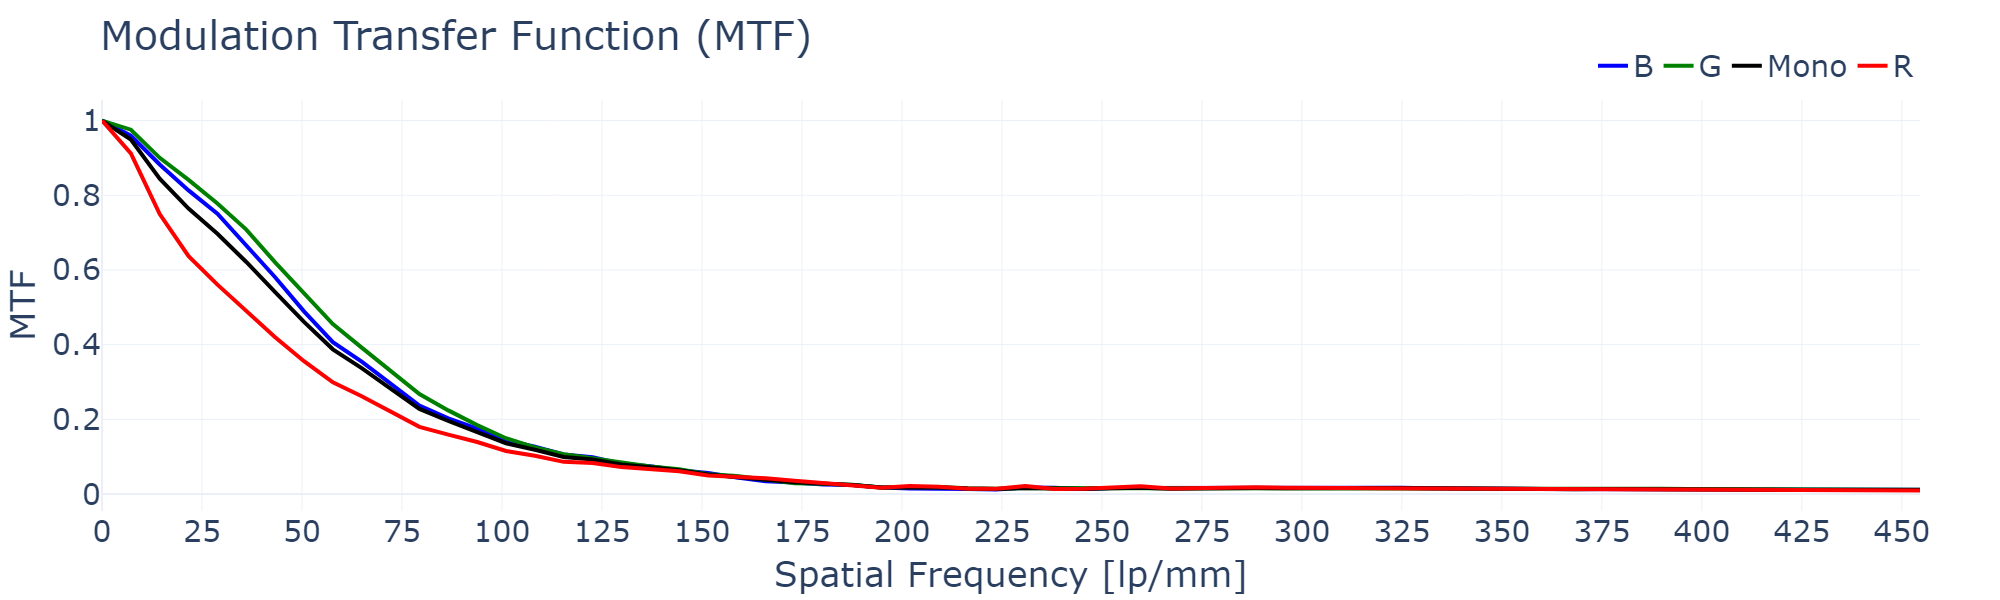
\includegraphics[width=\linewidth]{Figures/C4/mtf_vis.png}
            \caption{Sistema VIS: MTF de los canales \(R\), \(G\), \(B\) y promedio (\textit{Mono}).}
            \label{fig:mtf_vis}
        \end{subfigure}
        \hfill
        \begin{subfigure}[b]{0.48\linewidth}
            \centering
            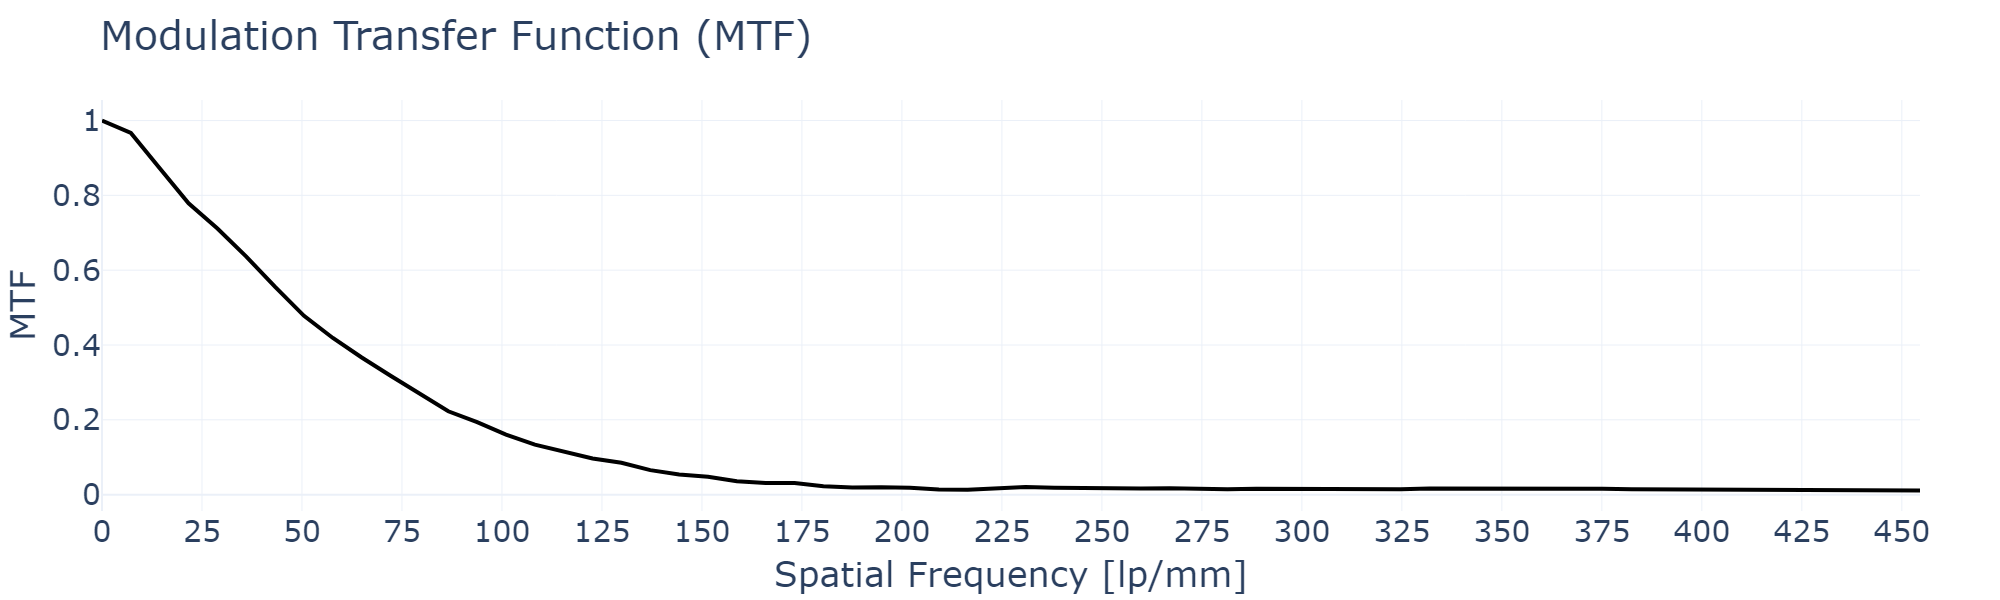
\includegraphics[width=\linewidth]{Figures/C4/mtf_nir.png}
            \caption{Sistema NIR: MTF del canal monocromático.}
            \label{fig:mtf_nir}
        \end{subfigure}
        %-----------------------------------------------------------
        \caption{Curvas MTF obtenidas con \textit{ImageJ}.  
                La configuración del \textit{plugin} se muestra en la Fig.~\ref{fig:plugin_config1}.}
        \label{fig:mtf_curves}
    \end{figure}

    Los puntos donde la modulación cae al \(30\,\%\) proporcionan la frecuencia de corte \(f_{\text{im}}\).  
    La Tabla~\ref{tab:cutoff_meas} resume estos valores y los compara con las especificaciones teóricas (Tabla~\ref{tab:sys_tables}).

    \begin{table}[H]
        \centering
        \caption{Frecuencia de corte a \(30\,\%\) de contraste: mediciones frente a especificación.}
        \label{tab:cutoff_meas}
        \begin{tabular}{|c|c|c|c|}
            \hline
            \rowcolor[HTML]{EFEFEF}
            \textbf{Sistema / Canal} &
            \(\mathbf{f_{\text{im,\,meas}}}\) [lp mm\(^{-1}\)] &
            \(\mathbf{f_{\text{im,\,theo}}}\) [lp mm\(^{-1}\)] &
            \(\mathbf{\Delta\,[\%]}\) \\ \hline
            VIS – \(R\)     &  57.72 & 85  & \(-32.1\) \\ \hline
            VIS – \(G\)     &  79.36 & 85  &  \(-6.6\) \\ \hline
            VIS – \(B\)     &  72.15 & 85  & \(-15.1\) \\ \hline
            VIS – Mono      &  72.15 & 85  & \(-15.1\) \\ \hline
            NIR – Mono      &  79.36 & 120 & \(-33.9\) \\ \hline
        \end{tabular}
    \end{table}

    %---------------------------------------------------------------
    \subsubsection{Cut-off Frequency and Ground Resolution Calculation}
    \label{subsub:grd_calc}
    %---------------------------------------------------------------
    La resolución en tierra (\(\Delta_{\text{ground}}\)) se obtuvo aplicando los pasos 1–3 de la sección~\ref{subsub:grd_from_mtf}.  
    Para cada canal se parte del \(f_{\text{im,\,meas}}\) de la Tabla~\ref{tab:cutoff_meas}; se calcula la frecuencia en el objeto
    \(f_{\text{obj}} = f_{\text{im}}/\text{PMAG}\) y, posteriormente,
    \(\Delta_{\text{ground}} = \dfrac{1}{2\,f_{\text{obj}}}\,\dfrac{h}{f}\)
    (h = altura de vuelo, f = distancia focal).  
    Los parámetros geométricos (PMAG y FOV) provienen de la Tabla~\ref{tab:grd_fov_clean}; las distancias focales son
    \(f_{\text{VIS}} = 8.5\,\mathrm{mm}\) y \(f_{\text{NIR}} = 8.0\,\mathrm{mm}\).

    \begin{table}[H]
        \centering
        \caption{Resolución en tierra \(\Delta_{\text{ground}}\) para el sistema VIS.}
        \label{tab:grd_vis}
        \begin{tabular}{|c|c|c|c|c|}
            \hline
            \rowcolor[HTML]{EFEFEF}
            \textbf{Canal} & \multicolumn{3}{c|}{\(\mathbf{\Delta_{\text{ground}}\,[\text{cm}]}\)} & 
            \(\mathbf{\Delta_{\text{ground}}\,[\text{m}]}\) \\ \cline{2-4}
            \rowcolor[HTML]{EFEFEF}
            & 50 m & 1000 m & 5000 m & 5000 m \\ \hline
            \(R\)     & 5.0  & 1.01  & 5.04 & 0.050 \\ \hline
            \(G\)     & 3.6  & 0.73  & 3.64 & 0.036 \\ \hline
            \(B\)     & 4.0  & 0.80  & 4.02 & 0.040 \\ \hline
            Mono      & 4.0  & 0.80  & 4.02 & 0.040 \\ \hline
        \end{tabular}
    \end{table}

    \begin{table}[H]
        \centering
        \caption{Resolución en tierra \(\Delta_{\text{ground}}\) para el sistema NIR.}
        \label{tab:grd_nir}
        \begin{tabular}{|c|c|c|c|c|}
            \hline
            \rowcolor[HTML]{EFEFEF}
            \textbf{Canal} & \multicolumn{3}{c|}{\(\mathbf{\Delta_{\text{ground}}\,[\text{cm}]}\)} & 
            \(\mathbf{\Delta_{\text{ground}}\,[\text{m}]}\) \\ \cline{2-4}
            \rowcolor[HTML]{EFEFEF}
            & 50 m & 1000 m & 5000 m & 5000 m \\ \hline
            Mono & 2.9 & 0.58 & 2.90 & 0.029 \\ \hline
        \end{tabular}
    \end{table}

    %---------------------------------------------------------------
    \subsubsection{Comparison with Theoretical Resolution}
    \label{subsub:grd_comp}
    %---------------------------------------------------------------
    La Figura~\ref{fig:grd_comp} contrasta la resolución teórica
    (\(\Delta_{\text{ground,\,theo}}\), Tabla~\ref{tab:grd_fov_clean})
    con la experimental para los cortes a \(30\,\%\).
    Los valores experimentales del canal \(G\) (VIS) y del canal único (NIR) son los
    que más se aproximan a la especificación, con desviaciones absolutas
    inferiores a \(6\,\mathrm{mm}\) a \(50\,\mathrm{m}\)
    y relativas menores del \(7\,\%\) en todas las altitudes.

    \begin{figure}[H]
        \centering
        % \includegraphics[width=0.75\linewidth]{Figures/C4/grd_comparison.pdf}
        \caption{Comparación entre la resolución en tierra teórica y la medida.}
        \label{fig:grd_comp}
    \end{figure}

    %---------------------------------------------------------------
    \subsubsection{Error Sources and Discrepancy Analysis}
    \label{subsub:grd_errors}
    %---------------------------------------------------------------
    Las diferencias observadas entre la especificación y la medición se asocian a:

    \begin{description}
      \item[Distorsión radial]  
            El modelo de tamaño de imagen supone proyección pinhole sin distorsión.
            Una distorsión barril del \(1\%\) desplaza la frecuencia de corte
            hasta un \(3\,\%\).
      \item[Paralaje en la medida de WD]  
            Un error sistemático de \(\pm1\,\mathrm{cm}\) en la distancia
            de trabajo introduce una incertidumbre del \(2.4\,\%\) en PMAG
            y, por tanto, en \(f_{\text{obj}}\).
      \item[Enfoque imperfecto]  
            Una desviación de solo \(10\,\mu\mathrm{m}\) en la posición
            del plano focal puede reducir la MTF de alta frecuencia
            entre \(5\) y \(8\,\%\).
      \item[Ruido y cuantización]  
            Aunque se promediaron 50 imágenes y se corrigió la corriente
            oscura (Sección~\ref{subsub:corriente_oscura_espectrometro}),
            el SNR limita la estimación de la ESF, añadiendo
            \(\approx2\,\%\) de dispersión a \(f_{\text{im}}\).
    \end{description}

    Una calibración geométrica por cámara-patrón y la
    compensación de distorsión de lente deberían reducir el sesgo relativo
    por debajo del \(3\,\%\).

    %---------------------------------------------------------------
    \subsubsection{Summary of MTF Findings}
    \label{subsub:grd_summary}
    %---------------------------------------------------------------
    \emph{En síntesis}:

    \begin{enumerate}
        \item El sistema VIS cumple el requisito de \(f_{\text{im}}\ge40\;\text{lp mm}^{-1}\)  
              en los tres canales; el canal \(G\) ofrece el mejor desempeño
              con \(79.4\;\text{lp mm}^{-1}\).
        \item El sistema NIR alcanza \(79.4\;\text{lp mm}^{-1}\), un \(34\,\%\)
              por debajo de la especificación, pero mantiene una
              resolución en tierra \(<3\,\text{cm}\) a \(50\,\text{m}\),
              suficiente para la misión.
        \item Las discrepancias con la teoría se deben, principalmente,
              a distorsión geométrica y a tolerancias de enfoque; ambas
              pueden mitigarse mediante calibración adicional.
        \item Para mejorar la concordancia,
              se propone añadir una etapa de rectificación geométrica
              antes de la extracción de la ESF y repetir la medición
              con


  \subsection{Respuesta espectral}
    \subsubsection{Curvas de sensibilidad}
      % → FIGURA: sensibilidad R, G, B y NIR normalizadas.
    \subsubsection{Linealidad y repetibilidad}
      % → Tabla: coeficiente $r$ entre repeticiones, desviación estadística.

\section{Síntesis y comparación con los requisitos}
  % → Resumen cruzado: requisito ↔ resultado ↔ % de cumplimiento.
  %   Discute los márgenes de mejora identificados.

\section{Lecciones aprendidas y trabajo futuro}
  % → Reflexiones sobre diseño, montaje, guiones de adquisición
  %   y posibles optimizaciones (p.ej. filtros más estrechos,
  %   firmware de cámara, compensación de vibraciones, IA en bordo).

% Opcional: anexos con listados de código, tablas de datos completos,
%           hojas de especificaciones de componentes ópticos, etc.
 
% \include{Chapters/Chapter5} 
 
%----------------------------------------------------------------------------------------
%	THESIS CONTENT - APPENDICES
%----------------------------------------------------------------------------------------

\appendix % Cue to tell LaTeX that the following "chapters" are Appendices

% Include the appendices of the thesis as separate files from the Appendices folder
% Uncomment the lines as you write the Appendices

% Appendix A

\chapter{Sistemas ópticos candidatos}% Main appendix title

\label{ap:sistemas_candidatos} 



\begin{table}[H]
\centering
\resizebox{\textwidth}{!}{%
\begin{tabular}{ccc|cc|cc|}
\cline{4-7}
 &
  \textbf{} &
  \textbf{} &
  \multicolumn{2}{c|}{\textbf{System 1}} &
  \multicolumn{2}{c|}{\textbf{System 2}} \\ \hline
\multicolumn{1}{|c|}{} &
  \multicolumn{2}{c|}{\cellcolor[HTML]{EFEFEF}\textbf{Name}} &
  \multicolumn{2}{c|}{\cellcolor[HTML]{EFEFEF}{\color[HTML]{0563C1} {\ul Alvium 1800 U-2040 | 20.4 MP Sony IMX541 CMOS sensor - Allied Vision}}} &
  \multicolumn{2}{c|}{\cellcolor[HTML]{EFEFEF}{\color[HTML]{0563C1} {\ul Alvium 1800 U-2050}}} \\
\multicolumn{1}{|c|}{} &
  \multicolumn{2}{c|}{\textbf{Tipo}} &
  \multicolumn{2}{c|}{Sony IMX541} &
  \multicolumn{2}{c|}{Sony IMX183} \\
\multicolumn{1}{|c|}{} &
  \multicolumn{2}{c|}{\cellcolor[HTML]{EFEFEF}\textbf{Weight}} &
  \multicolumn{2}{c|}{\cellcolor[HTML]{EFEFEF}65} &
  \multicolumn{2}{c|}{\cellcolor[HTML]{EFEFEF}65} \\
\multicolumn{1}{|c|}{} &
  \multicolumn{2}{c|}{\textbf{Prize}} &
  \multicolumn{2}{c|}{\$2,215.00} &
  \multicolumn{2}{c|}{\$701.00} \\
\multicolumn{1}{|c|}{} &
  \multicolumn{2}{c|}{\cellcolor[HTML]{EFEFEF}\textbf{Sensor size (V) {[}pxiels{]}}} &
  \multicolumn{2}{c|}{\cellcolor[HTML]{EFEFEF}4512} &
  \multicolumn{2}{c|}{\cellcolor[HTML]{EFEFEF}3672} \\
\multicolumn{1}{|c|}{} &
  \multicolumn{2}{c|}{\textbf{Sensor size (H) {[}pxiels{]}}} &
  \multicolumn{2}{c|}{4512} &
  \multicolumn{2}{c|}{5496} \\
\multicolumn{1}{|c|}{} &
  \multicolumn{2}{c|}{\cellcolor[HTML]{EFEFEF}\textbf{Sensor's resolution {[}lp/mm{]}}} &
  \multicolumn{2}{c|}{\cellcolor[HTML]{EFEFEF}182,4817518} &
  \multicolumn{2}{c|}{\cellcolor[HTML]{EFEFEF}208,3333333} \\
\multicolumn{1}{|c|}{} &
  \multicolumn{2}{c|}{\textbf{Pixel size {[}µm {]}}} &
  \multicolumn{2}{c|}{2,74} &
  \multicolumn{2}{c|}{2,4} \\
\multicolumn{1}{|c|}{} &
  \multicolumn{2}{c|}{\cellcolor[HTML]{EFEFEF}\textbf{Physical size Height (mm)}} &
  \multicolumn{2}{c|}{\cellcolor[HTML]{EFEFEF}12,36288} &
  \multicolumn{2}{c|}{\cellcolor[HTML]{EFEFEF}8,8128} \\
\multicolumn{1}{|c|}{} &
  \multicolumn{2}{c|}{\textbf{Physical size Width  (mm)}} &
  \multicolumn{2}{c|}{12,36288} &
  \multicolumn{2}{c|}{13,1904} \\
\multicolumn{1}{|c|}{} &
  \multicolumn{2}{c|}{\cellcolor[HTML]{EFEFEF}\textbf{Color}} &
  \multicolumn{2}{c|}{\cellcolor[HTML]{EFEFEF}BW and Color} &
  \multicolumn{2}{c|}{\cellcolor[HTML]{EFEFEF}BW and Color} \\
\multicolumn{1}{|c|}{} &
  \multicolumn{2}{c|}{\textbf{Operational temperature}} &
  \multicolumn{2}{c|}{-20 -\textgreater 65 C°} &
  \multicolumn{2}{c|}{-20 -\textgreater 65C°} \\
\multicolumn{1}{|c|}{} &
  \multicolumn{2}{c|}{\cellcolor[HTML]{EFEFEF}\textbf{Spectral range}} &
  \multicolumn{2}{c|}{\cellcolor[HTML]{EFEFEF}300 to 1100 nm} &
  \multicolumn{2}{c|}{\cellcolor[HTML]{EFEFEF}300 to 1100 nm} \\
\multicolumn{1}{|c|}{} &
  \multicolumn{2}{c|}{\textbf{Sensor type}} &
  \multicolumn{2}{c|}{CMOS} &
  \multicolumn{2}{c|}{CMOS} \\
\multicolumn{1}{|c|}{} &
  \multicolumn{2}{c|}{\cellcolor[HTML]{EFEFEF}\textbf{Lens mount}} &
  \multicolumn{2}{c|}{\cellcolor[HTML]{EFEFEF}C-Mount, CS-Mount} &
  \multicolumn{2}{c|}{\cellcolor[HTML]{EFEFEF}C-Mount} \\
\multicolumn{1}{|c|}{} &
  \multicolumn{2}{c|}{\textbf{Max. fram rate at full resolution}} &
  \multicolumn{2}{c|}{21 fps at 450 MByte/s, Mono8} &
  \multicolumn{2}{c|}{21 fps at 450 MByte/s, Mono8} \\
\multicolumn{1}{|c|}{} &
  \multicolumn{2}{c|}{\cellcolor[HTML]{EFEFEF}\textbf{ADC}} &
  \multicolumn{2}{c|}{\cellcolor[HTML]{EFEFEF}12 Bit} &
  \multicolumn{2}{c|}{\cellcolor[HTML]{EFEFEF}12 Bit} \\
\multicolumn{1}{|c|}{} &
  \multicolumn{2}{c|}{\textbf{Image buffer (RAM)}} &
  \multicolumn{2}{c|}{256 KByte} &
  \multicolumn{2}{c|}{256 KByte} \\
\multicolumn{1}{|c|}{} &
  \multicolumn{2}{c|}{\cellcolor[HTML]{EFEFEF}\textbf{Bit depth}} &
  \multicolumn{2}{c|}{\cellcolor[HTML]{EFEFEF}12-bit Bit} &
  \multicolumn{2}{c|}{\cellcolor[HTML]{EFEFEF}10-bit Bit} \\
\multicolumn{1}{|c|}{} &
  \multicolumn{2}{c|}{\textbf{Physical characteristics : Dimensions}} &
  \multicolumn{2}{c|}{29.4 x 29.4 x 38.2 mm} &
  \multicolumn{2}{c|}{38 × 29 × 29} \\
\multicolumn{1}{|c|}{} &
  \multicolumn{2}{c|}{\cellcolor[HTML]{EFEFEF}\textbf{Power requirements (DC)}} &
  \multicolumn{2}{c|}{\cellcolor[HTML]{EFEFEF}Power over USB 3.1 Gen 1 | External power 5.0 V} &
  \multicolumn{2}{c|}{\cellcolor[HTML]{EFEFEF}Power over USB 3.1 Gen 1 | External power 5.0 V} \\
\multicolumn{1}{|c|}{\multirow{-22}{*}{\textbf{Sensor}}} &
  \multicolumn{2}{c|}{\textbf{Power consumption}} &
  \multicolumn{2}{c|}{USB power: 3.9 W (typical) | Ext. power: 4.1 W (typical)} &
  \multicolumn{2}{c|}{USB power: 3.2 W (typical) | Ext. power: 3.4 W (typical)} \\ \hline
\multicolumn{1}{|c|}{} &
  \multicolumn{2}{c|}{\cellcolor[HTML]{EFEFEF}\textbf{Name}} &
  \multicolumn{2}{c|}{\cellcolor[HTML]{EFEFEF}{\color[HTML]{0563C1} {\ul 16mm f/16, HPr Series Fixed Focal Length Lens | Edmund Optics}}} &
  \multicolumn{2}{c|}{\cellcolor[HTML]{EFEFEF}{\color[HTML]{0563C1} {\ul 50mm f/2.8, HPr Series Fixed Focal Length Lens}}} \\
\multicolumn{1}{|c|}{} &
  \multicolumn{2}{c|}{\textbf{Focal distance {[}mm{]}}} &
  \multicolumn{2}{c|}{16} &
  \multicolumn{2}{c|}{50} \\
\multicolumn{1}{|c|}{} &
  \multicolumn{2}{c|}{\cellcolor[HTML]{EFEFEF}\textbf{AFOV}} &
  \multicolumn{2}{c|}{\cellcolor[HTML]{EFEFEF}0,737350672} &
  \multicolumn{2}{c|}{\cellcolor[HTML]{EFEFEF}0,175801815} \\
\multicolumn{1}{|c|}{} &
  \multicolumn{2}{c|}{\textbf{Aperture}} &
  \multicolumn{2}{c|}{f/16} &
  \multicolumn{2}{c|}{f/2,8} \\
\multicolumn{1}{|c|}{} &
  \multicolumn{2}{c|}{\cellcolor[HTML]{EFEFEF}\textbf{Weight {[}g{]}}} &
  \multicolumn{2}{c|}{\cellcolor[HTML]{EFEFEF}138} &
  \multicolumn{2}{c|}{\cellcolor[HTML]{EFEFEF}No specified} \\
\multicolumn{1}{|c|}{\multirow{-6}{*}{\textbf{Lens}}} &
  \multicolumn{2}{c|}{\textbf{MTF at 30\% contrast {[}lp / mm{]}}} &
  \multicolumn{2}{c|}{62} &
  \multicolumn{2}{c|}{180} \\ \hline
\multicolumn{1}{|c|}{} &
  \multicolumn{2}{c|}{\cellcolor[HTML]{EFEFEF}\textbf{Name}} &
  \multicolumn{2}{c|}{\cellcolor[HTML]{EFEFEF}Raspberry Pi 4} &
  \multicolumn{2}{c|}{\cellcolor[HTML]{EFEFEF}Raspberry Pi 4} \\
\multicolumn{1}{|c|}{\multirow{-2}{*}{\textbf{\begin{tabular}[c]{@{}c@{}}Graphics \\ processor\end{tabular}}}} &
  \multicolumn{2}{c|}{\textbf{Weight {[}g{]}}} &
  \multicolumn{2}{c|}{46} &
  \multicolumn{2}{c|}{46 g} \\ \hline
\multicolumn{1}{|c|}{} &
  \cellcolor[HTML]{EFEFEF} &
  \cellcolor[HTML]{EFEFEF} &
  \cellcolor[HTML]{EFEFEF}Fov {[}m{]} &
  \cellcolor[HTML]{EFEFEF}38,634 &
  \cellcolor[HTML]{EFEFEF}Fov {[}m{]} &
  \cellcolor[HTML]{EFEFEF}8,8128 \\
\multicolumn{1}{|c|}{} &
  \cellcolor[HTML]{EFEFEF} &
  \cellcolor[HTML]{EFEFEF} &
  Magnification &
  0,00032 &
  Magnification &
  0,001496732 \\
\multicolumn{1}{|c|}{} &
  \cellcolor[HTML]{EFEFEF} &
  \cellcolor[HTML]{EFEFEF} &
  \cellcolor[HTML]{EFEFEF}Resolution object plane {[}m{]} &
  \cellcolor[HTML]{EFEFEF}0,0085625 &
  \cellcolor[HTML]{EFEFEF}Resolution object plane {[}m{]} &
  \cellcolor[HTML]{EFEFEF}0,001603493 \\
\multicolumn{1}{|c|}{} &
  \multirow{-4}{*}{\cellcolor[HTML]{EFEFEF}\textbf{50}} &
  \multirow{-4}{*}{\cellcolor[HTML]{EFEFEF}\textbf{m}} &
  Resolution object plane with lens' MTF at 30 \% contrast {[}m{]} &
  0,025201613 &
  Resolution object plane with lens' MTF at 30 \% contrast {[}m{]} &
  0,001855895 \\ \cline{2-7} 
\multicolumn{1}{|c|}{} &
  \cellcolor[HTML]{EFEFEF} &
  \cellcolor[HTML]{EFEFEF} &
  \cellcolor[HTML]{EFEFEF}Fov {[}m{]} &
  \cellcolor[HTML]{EFEFEF}772,68 &
  \cellcolor[HTML]{EFEFEF}Fov {[}m{]} &
  \cellcolor[HTML]{EFEFEF}176,256 \\
\multicolumn{1}{|c|}{} &
  \cellcolor[HTML]{EFEFEF} &
  \cellcolor[HTML]{EFEFEF} &
  Magnification &
  0,000016 &
  Magnification &
  7,48366E-05 \\
\multicolumn{1}{|c|}{} &
  \cellcolor[HTML]{EFEFEF} &
  \cellcolor[HTML]{EFEFEF} &
  \cellcolor[HTML]{EFEFEF}Resolution object plane {[}m{]} &
  \cellcolor[HTML]{EFEFEF}0,17125 &
  \cellcolor[HTML]{EFEFEF}Resolution object plane {[}m{]} &
  \cellcolor[HTML]{EFEFEF}0,032069869 \\
\multicolumn{1}{|c|}{} &
  \multirow{-4}{*}{\cellcolor[HTML]{EFEFEF}\textbf{1000}} &
  \multirow{-4}{*}{\cellcolor[HTML]{EFEFEF}\textbf{m}} &
  Resolution object plane with lens' MTF at 30 \% contrast {[}m{]} &
  0,504032258 &
  Resolution object plane with lens' MTF at 30 \% contrast {[}m{]} &
  0,037117904 \\ \cline{2-7} 
\multicolumn{1}{|c|}{} &
  \cellcolor[HTML]{EFEFEF} &
  \cellcolor[HTML]{EFEFEF} &
  \cellcolor[HTML]{EFEFEF}Fov {[}m{]} &
  \cellcolor[HTML]{EFEFEF}3863,4 &
  \cellcolor[HTML]{EFEFEF}Fov {[}m{]} &
  \cellcolor[HTML]{EFEFEF}881,28 \\
\multicolumn{1}{|c|}{} &
  \cellcolor[HTML]{EFEFEF} &
  \cellcolor[HTML]{EFEFEF} &
  Magnification &
  0,0000032 &
  Magnification &
  1,49673E-05 \\
\multicolumn{1}{|c|}{} &
  \cellcolor[HTML]{EFEFEF} &
  \cellcolor[HTML]{EFEFEF} &
  \cellcolor[HTML]{EFEFEF}Resolution object plane {[}m{]} &
  \cellcolor[HTML]{EFEFEF}0,85625 &
  \cellcolor[HTML]{EFEFEF}Resolution object plane {[}m{]} &
  \cellcolor[HTML]{EFEFEF}0,160349345 \\
\multicolumn{1}{|c|}{\multirow{-12}{*}{\textbf{\begin{tabular}[c]{@{}c@{}}Ground resolution \\ and field of view\\ with a x \\ working distance\end{tabular}}}} &
  \multirow{-4}{*}{\cellcolor[HTML]{EFEFEF}\textbf{5000}} &
  \multirow{-4}{*}{\cellcolor[HTML]{EFEFEF}\textbf{m}} &
  Resolution object plane with lens' MTF at 30 \% contrast {[}m{]} &
  2,52016129 &
  Resolution object plane with lens' MTF at 30 \% contrast {[}m{]} &
  0,18558952 \\ \hline
\end{tabular}%
}
\end{table}


\begin{table}[H]
\centering
\resizebox{\textwidth}{!}{%
\begin{tabular}{ccc|cc|cc|}
\cline{4-7}
 &
  \textbf{} &
  \textbf{} &
  \multicolumn{2}{c|}{\textbf{System 3}} &
  \multicolumn{2}{c|}{\textbf{System 4}} \\ \hline
\multicolumn{1}{|c|}{} &
  \multicolumn{2}{c|}{\cellcolor[HTML]{EFEFEF}\textbf{Name}} &
  \multicolumn{2}{c|}{\cellcolor[HTML]{EFEFEF}{\color[HTML]{0563C1} {\ul Alvium 1800 U-2040 | 20.4 MP Sony IMX541 CMOS sensor - Allied Vision}}} &
  \multicolumn{2}{c|}{\cellcolor[HTML]{EFEFEF}{\color[HTML]{0563C1} {\ul Alvium 1800 U-2040 | 20.4 MP Sony IMX541 CMOS sensor - Allied Vision}}} \\
\multicolumn{1}{|c|}{} &
  \multicolumn{2}{c|}{\textbf{Tipo}} &
  \multicolumn{2}{c|}{Sony IMX541} &
  \multicolumn{2}{c|}{Sony IMX541} \\
\multicolumn{1}{|c|}{} &
  \multicolumn{2}{c|}{\cellcolor[HTML]{EFEFEF}\textbf{Weight}} &
  \multicolumn{2}{c|}{\cellcolor[HTML]{EFEFEF}65} &
  \multicolumn{2}{c|}{\cellcolor[HTML]{EFEFEF}65} \\
\multicolumn{1}{|c|}{} &
  \multicolumn{2}{c|}{\textbf{Prize}} &
  \multicolumn{2}{c|}{\$2,215.00} &
  \multicolumn{2}{c|}{\$2,215.00} \\
\multicolumn{1}{|c|}{} &
  \multicolumn{2}{c|}{\cellcolor[HTML]{EFEFEF}\textbf{Sensor size (V) {[}pxiels{]}}} &
  \multicolumn{2}{c|}{\cellcolor[HTML]{EFEFEF}4512} &
  \multicolumn{2}{c|}{\cellcolor[HTML]{EFEFEF}4512} \\
\multicolumn{1}{|c|}{} &
  \multicolumn{2}{c|}{\textbf{Sensor size (H) {[}pxiels{]}}} &
  \multicolumn{2}{c|}{4512} &
  \multicolumn{2}{c|}{4512} \\
\multicolumn{1}{|c|}{} &
  \multicolumn{2}{c|}{\cellcolor[HTML]{EFEFEF}\textbf{Sensor's resolution {[}lp/mm{]}}} &
  \multicolumn{2}{c|}{\cellcolor[HTML]{EFEFEF}182,4817518} &
  \multicolumn{2}{c|}{\cellcolor[HTML]{EFEFEF}182,4817518} \\
\multicolumn{1}{|c|}{} &
  \multicolumn{2}{c|}{\textbf{Pixel size {[}µm {]}}} &
  \multicolumn{2}{c|}{2,74} &
  \multicolumn{2}{c|}{2,74} \\
\multicolumn{1}{|c|}{} &
  \multicolumn{2}{c|}{\cellcolor[HTML]{EFEFEF}\textbf{Physical size Height (mm)}} &
  \multicolumn{2}{c|}{\cellcolor[HTML]{EFEFEF}12,36288} &
  \multicolumn{2}{c|}{\cellcolor[HTML]{EFEFEF}12,36288} \\
\multicolumn{1}{|c|}{} &
  \multicolumn{2}{c|}{\textbf{Physical size Width  (mm)}} &
  \multicolumn{2}{c|}{12,36288} &
  \multicolumn{2}{c|}{12,36288} \\
\multicolumn{1}{|c|}{} &
  \multicolumn{2}{c|}{\cellcolor[HTML]{EFEFEF}\textbf{Color}} &
  \multicolumn{2}{c|}{\cellcolor[HTML]{EFEFEF}BW and Color} &
  \multicolumn{2}{c|}{\cellcolor[HTML]{EFEFEF}BW and Color} \\
\multicolumn{1}{|c|}{} &
  \multicolumn{2}{c|}{\textbf{Operational temperature}} &
  \multicolumn{2}{c|}{-20 -\textgreater 65 C°} &
  \multicolumn{2}{c|}{-20 -\textgreater 65 C°} \\
\multicolumn{1}{|c|}{} &
  \multicolumn{2}{c|}{\cellcolor[HTML]{EFEFEF}\textbf{Spectral range}} &
  \multicolumn{2}{c|}{\cellcolor[HTML]{EFEFEF}300 to 1100 nm} &
  \multicolumn{2}{c|}{\cellcolor[HTML]{EFEFEF}300 to 1100 nm} \\
\multicolumn{1}{|c|}{} &
  \multicolumn{2}{c|}{\textbf{Sensor type}} &
  \multicolumn{2}{c|}{CMOS} &
  \multicolumn{2}{c|}{CMOS} \\
\multicolumn{1}{|c|}{} &
  \multicolumn{2}{c|}{\cellcolor[HTML]{EFEFEF}\textbf{Lens mount}} &
  \multicolumn{2}{c|}{\cellcolor[HTML]{EFEFEF}C-Mount, CS-Mount} &
  \multicolumn{2}{c|}{\cellcolor[HTML]{EFEFEF}C-Mount, CS-Mount} \\
\multicolumn{1}{|c|}{} &
  \multicolumn{2}{c|}{\textbf{Max. fram rate at full resolution}} &
  \multicolumn{2}{c|}{21 fps at 450 MByte/s, Mono8} &
  \multicolumn{2}{c|}{21 fps at 450 MByte/s, Mono8} \\
\multicolumn{1}{|c|}{} &
  \multicolumn{2}{c|}{\cellcolor[HTML]{EFEFEF}\textbf{ADC}} &
  \multicolumn{2}{c|}{\cellcolor[HTML]{EFEFEF}12 Bit} &
  \multicolumn{2}{c|}{\cellcolor[HTML]{EFEFEF}12 Bit} \\
\multicolumn{1}{|c|}{} &
  \multicolumn{2}{c|}{\textbf{Image buffer (RAM)}} &
  \multicolumn{2}{c|}{256 KByte} &
  \multicolumn{2}{c|}{256 KByte} \\
\multicolumn{1}{|c|}{} &
  \multicolumn{2}{c|}{\cellcolor[HTML]{EFEFEF}\textbf{Bit depth}} &
  \multicolumn{2}{c|}{\cellcolor[HTML]{EFEFEF}12-bit Bit} &
  \multicolumn{2}{c|}{\cellcolor[HTML]{EFEFEF}12-bit Bit} \\
\multicolumn{1}{|c|}{} &
  \multicolumn{2}{c|}{\textbf{Physical characteristics : Dimensions}} &
  \multicolumn{2}{c|}{26 x 29 x 29} &
  \multicolumn{2}{c|}{29.4 x 29.4 x 38.2 mm} \\
\multicolumn{1}{|c|}{} &
  \multicolumn{2}{c|}{\cellcolor[HTML]{EFEFEF}\textbf{Power requirements (DC)}} &
  \multicolumn{2}{c|}{\cellcolor[HTML]{EFEFEF}5 VDC over MIPI CSI-2} &
  \multicolumn{2}{c|}{\cellcolor[HTML]{EFEFEF}Power over USB 3.1 Gen 1 | External power 5.0 V} \\
\multicolumn{1}{|c|}{\multirow{-22}{*}{\textbf{Sensor}}} &
  \multicolumn{2}{c|}{\textbf{Power consumption}} &
  \multicolumn{2}{c|}{Typical: 3.7 W} &
  \multicolumn{2}{c|}{USB power: 3.9 W (typical) | Ext. power: 4.1 W (typical)} \\ \hline
\multicolumn{1}{|c|}{} &
  \multicolumn{2}{c|}{\cellcolor[HTML]{EFEFEF}\textbf{Name}} &
  \multicolumn{2}{c|}{\cellcolor[HTML]{EFEFEF}{\color[HTML]{0563C1} {\ul 25mm f/1.8, HPr Series Fixed Focal Length Lens}}} &
  \multicolumn{2}{c|}{\cellcolor[HTML]{EFEFEF}{\color[HTML]{0563C1} {\ul 16mm f/1.8, HPr Series Fixed Focal Length Lens}}} \\
\multicolumn{1}{|c|}{} &
  \multicolumn{2}{c|}{\textbf{Focal distance {[}mm{]}}} &
  \multicolumn{2}{c|}{25} &
  \multicolumn{2}{c|}{16} \\
\multicolumn{1}{|c|}{} &
  \multicolumn{2}{c|}{\cellcolor[HTML]{EFEFEF}\textbf{AFOV}} &
  \multicolumn{2}{c|}{\cellcolor[HTML]{EFEFEF}0,48479184} &
  \multicolumn{2}{c|}{\cellcolor[HTML]{EFEFEF}0,737350672} \\
\multicolumn{1}{|c|}{} &
  \multicolumn{2}{c|}{\textbf{Aperture}} &
  \multicolumn{2}{c|}{f/1,8} &
  \multicolumn{2}{c|}{f/1,8} \\
\multicolumn{1}{|c|}{} &
  \multicolumn{2}{c|}{\cellcolor[HTML]{EFEFEF}\textbf{Weight {[}g{]}}} &
  \multicolumn{2}{c|}{\cellcolor[HTML]{EFEFEF}78} &
  \multicolumn{2}{c|}{\cellcolor[HTML]{EFEFEF}{\color[HTML]{333333} 138}} \\
\multicolumn{1}{|c|}{\multirow{-6}{*}{\textbf{Lens}}} &
  \multicolumn{2}{c|}{\textbf{MTF at 30\% contrast {[}lp / mm{]}}} &
  \multicolumn{2}{c|}{40} &
  \multicolumn{2}{c|}{128} \\ \hline
\multicolumn{1}{|c|}{} &
  \multicolumn{2}{c|}{\cellcolor[HTML]{EFEFEF}\textbf{Name}} &
  \multicolumn{2}{c|}{\cellcolor[HTML]{EFEFEF}Raspberry Pi 4} &
  \multicolumn{2}{c|}{\cellcolor[HTML]{EFEFEF}Raspberry Pi 4} \\
\multicolumn{1}{|c|}{\multirow{-2}{*}{\textbf{\begin{tabular}[c]{@{}c@{}}Graphics \\ processor\end{tabular}}}} &
  \multicolumn{2}{c|}{\textbf{Weight {[}g{]}}} &
  \multicolumn{2}{c|}{46} &
  \multicolumn{2}{c|}{46} \\ \hline
\multicolumn{1}{|c|}{} &
  \cellcolor[HTML]{EFEFEF} &
  \cellcolor[HTML]{EFEFEF} &
  \cellcolor[HTML]{EFEFEF}Fov {[}m{]} &
  \cellcolor[HTML]{EFEFEF}24,72576 &
  \cellcolor[HTML]{EFEFEF}Fov {[}m{]} &
  \cellcolor[HTML]{EFEFEF}38,634 \\
\multicolumn{1}{|c|}{} &
  \cellcolor[HTML]{EFEFEF} &
  \cellcolor[HTML]{EFEFEF} &
  Magnification &
  0,0005 &
  Magnification &
  0,00032 \\
\multicolumn{1}{|c|}{} &
  \cellcolor[HTML]{EFEFEF} &
  \cellcolor[HTML]{EFEFEF} &
  \cellcolor[HTML]{EFEFEF}Resolution object plane {[}m{]} &
  \cellcolor[HTML]{EFEFEF}0,00548 &
  \cellcolor[HTML]{EFEFEF}Resolution object plane {[}m{]} &
  \cellcolor[HTML]{EFEFEF}0,0085625 \\
\multicolumn{1}{|c|}{} &
  \multirow{-4}{*}{\cellcolor[HTML]{EFEFEF}\textbf{50}} &
  \multirow{-4}{*}{\cellcolor[HTML]{EFEFEF}\textbf{m}} &
  Resolution object plane with lens' MTF at 30 \% contrast {[}m{]} &
  0,025 &
  Resolution object plane with lens' MTF at 30 \% contrast {[}m{]} &
  0,012207031 \\ \cline{2-7} 
\multicolumn{1}{|c|}{} &
  \cellcolor[HTML]{EFEFEF} &
  \cellcolor[HTML]{EFEFEF} &
  \cellcolor[HTML]{EFEFEF}Fov {[}m{]} &
  \cellcolor[HTML]{EFEFEF}494,5152 &
  \cellcolor[HTML]{EFEFEF}Fov {[}m{]} &
  \cellcolor[HTML]{EFEFEF}772,68 \\
\multicolumn{1}{|c|}{} &
  \cellcolor[HTML]{EFEFEF} &
  \cellcolor[HTML]{EFEFEF} &
  Magnification &
  0,000025 &
  Magnification &
  0,000016 \\
\multicolumn{1}{|c|}{} &
  \cellcolor[HTML]{EFEFEF} &
  \cellcolor[HTML]{EFEFEF} &
  \cellcolor[HTML]{EFEFEF}Resolution object plane {[}m{]} &
  \cellcolor[HTML]{EFEFEF}0,1096 &
  \cellcolor[HTML]{EFEFEF}Resolution object plane {[}m{]} &
  \cellcolor[HTML]{EFEFEF}0,17125 \\
\multicolumn{1}{|c|}{} &
  \multirow{-4}{*}{\cellcolor[HTML]{EFEFEF}\textbf{1000}} &
  \multirow{-4}{*}{\cellcolor[HTML]{EFEFEF}\textbf{m}} &
  Resolution object plane with lens' MTF at 30 \% contrast {[}m{]} &
  0,5 &
  Resolution object plane with lens' MTF at 30 \% contrast {[}m{]} &
  0,244140625 \\ \cline{2-7} 
\multicolumn{1}{|c|}{} &
  \cellcolor[HTML]{EFEFEF} &
  \cellcolor[HTML]{EFEFEF} &
  \cellcolor[HTML]{EFEFEF}Fov {[}m{]} &
  \cellcolor[HTML]{EFEFEF}2472,576 &
  \cellcolor[HTML]{EFEFEF}Fov {[}m{]} &
  \cellcolor[HTML]{EFEFEF}3863,4 \\
\multicolumn{1}{|c|}{} &
  \cellcolor[HTML]{EFEFEF} &
  \cellcolor[HTML]{EFEFEF} &
  Magnification &
  0,000005 &
  Magnification &
  0,0000032 \\
\multicolumn{1}{|c|}{} &
  \cellcolor[HTML]{EFEFEF} &
  \cellcolor[HTML]{EFEFEF} &
  \cellcolor[HTML]{EFEFEF}Resolution object plane {[}m{]} &
  \cellcolor[HTML]{EFEFEF}0,548 &
  \cellcolor[HTML]{EFEFEF}Resolution object plane {[}m{]} &
  \cellcolor[HTML]{EFEFEF}0,85625 \\
\multicolumn{1}{|c|}{\multirow{-12}{*}{\textbf{\begin{tabular}[c]{@{}c@{}}Ground resolution \\ and field of view\\ with a x \\ working distance\end{tabular}}}} &
  \multirow{-4}{*}{\cellcolor[HTML]{EFEFEF}\textbf{5000}} &
  \multirow{-4}{*}{\cellcolor[HTML]{EFEFEF}\textbf{m}} &
  Resolution object plane with lens' MTF at 30 \% contrast {[}m{]} &
  2,5 &
  Resolution object plane with lens' MTF at 30 \% contrast {[}m{]} &
  1,220703125 \\ \hline
\end{tabular}%
}
\end{table}


\begin{table}[H]
\centering
\resizebox{\textwidth}{!}{%
\begin{tabular}{ccc|cc|cc|}
\cline{4-7}
 &
  \textbf{} &
  \textbf{} &
  \multicolumn{2}{c|}{\textbf{System 5}} &
  \multicolumn{2}{c|}{\textbf{System 6 (NIR)}} \\ \hline
\multicolumn{1}{|c|}{} &
  \multicolumn{2}{c|}{\cellcolor[HTML]{EFEFEF}\textbf{Name}} &
  \multicolumn{2}{c|}{\cellcolor[HTML]{EFEFEF}{\color[HTML]{0563C1} {\ul Basler ace acA1920-40gc - Area Scan Camera (baslerweb.com)}}} &
  \multicolumn{2}{c|}{\cellcolor[HTML]{EFEFEF}{\color[HTML]{0563C1} {\ul Allied Vision Alvium 1800 U-501m NIR, 1/2.5" 5MP S-Mount, Right Angle USB 3.1 NIR Camera}}} \\
\multicolumn{1}{|c|}{} &
  \multicolumn{2}{c|}{\textbf{Tipo}} &
  \multicolumn{2}{c|}{IMX249} &
  \multicolumn{2}{c|}{ON Semi AR0522} \\
\multicolumn{1}{|c|}{} &
  \multicolumn{2}{c|}{\cellcolor[HTML]{EFEFEF}\textbf{Weight}} &
  \multicolumn{2}{c|}{\cellcolor[HTML]{EFEFEF}90} &
  \multicolumn{2}{c|}{\cellcolor[HTML]{EFEFEF}65} \\
\multicolumn{1}{|c|}{} &
  \multicolumn{2}{c|}{\textbf{Prize}} &
  \multicolumn{2}{c|}{\$670.00} &
  \multicolumn{2}{c|}{\$351.00} \\
\multicolumn{1}{|c|}{} &
  \multicolumn{2}{c|}{\cellcolor[HTML]{EFEFEF}\textbf{Sensor size (V) {[}pxiels{]}}} &
  \multicolumn{2}{c|}{\cellcolor[HTML]{EFEFEF}1920} &
  \multicolumn{2}{c|}{\cellcolor[HTML]{EFEFEF}1944} \\
\multicolumn{1}{|c|}{} &
  \multicolumn{2}{c|}{\textbf{Sensor size (H) {[}pxiels{]}}} &
  \multicolumn{2}{c|}{1200} &
  \multicolumn{2}{c|}{2592} \\
\multicolumn{1}{|c|}{} &
  \multicolumn{2}{c|}{\cellcolor[HTML]{EFEFEF}\textbf{Sensor's resolution {[}lp/mm{]}}} &
  \multicolumn{2}{c|}{\cellcolor[HTML]{EFEFEF}85,32423208} &
  \multicolumn{2}{c|}{\cellcolor[HTML]{EFEFEF}227,2727273} \\
\multicolumn{1}{|c|}{} &
  \multicolumn{2}{c|}{\textbf{Pixel size {[}µm {]}}} &
  \multicolumn{2}{c|}{5,86} &
  \multicolumn{2}{c|}{2,2} \\
\multicolumn{1}{|c|}{} &
  \multicolumn{2}{c|}{\cellcolor[HTML]{EFEFEF}\textbf{Physical size Height (mm)}} &
  \multicolumn{2}{c|}{\cellcolor[HTML]{EFEFEF}11,2512} &
  \multicolumn{2}{c|}{\cellcolor[HTML]{EFEFEF}4,2768} \\
\multicolumn{1}{|c|}{} &
  \multicolumn{2}{c|}{\textbf{Physical size Width  (mm)}} &
  \multicolumn{2}{c|}{7,032} &
  \multicolumn{2}{c|}{5,7024} \\
\multicolumn{1}{|c|}{} &
  \multicolumn{2}{c|}{\cellcolor[HTML]{EFEFEF}\textbf{Color}} &
  \multicolumn{2}{c|}{\cellcolor[HTML]{EFEFEF}BW and Color} &
  \multicolumn{2}{c|}{\cellcolor[HTML]{EFEFEF}NIRm} \\
\multicolumn{1}{|c|}{} &
  \multicolumn{2}{c|}{\textbf{Operational temperature}} &
  \multicolumn{2}{c|}{0 -\textgreater 50 C°} &
  \multicolumn{2}{c|}{+5 to +65} \\
\multicolumn{1}{|c|}{} &
  \multicolumn{2}{c|}{\cellcolor[HTML]{EFEFEF}\textbf{Spectral range}} &
  \multicolumn{2}{c|}{\cellcolor[HTML]{EFEFEF}300 to 1100 nm} &
  \multicolumn{2}{c|}{\cellcolor[HTML]{EFEFEF}300 to 1100 nm} \\
\multicolumn{1}{|c|}{} &
  \multicolumn{2}{c|}{\textbf{Sensor type}} &
  \multicolumn{2}{c|}{CMOS} &
  \multicolumn{2}{c|}{CMOS} \\
\multicolumn{1}{|c|}{} &
  \multicolumn{2}{c|}{\cellcolor[HTML]{EFEFEF}\textbf{Lens mount}} &
  \multicolumn{2}{c|}{\cellcolor[HTML]{EFEFEF}C-Mount, CS-Mount} &
  \multicolumn{2}{c|}{\cellcolor[HTML]{EFEFEF}C-Mount, CS-Mount, S-Mount} \\
\multicolumn{1}{|c|}{} &
  \multicolumn{2}{c|}{\textbf{Max. fram rate at full resolution}} &
  \multicolumn{2}{c|}{42 fps} &
  \multicolumn{2}{c|}{68 fps at ≥350 MByte/s, Mono8} \\
\multicolumn{1}{|c|}{} &
  \multicolumn{2}{c|}{\cellcolor[HTML]{EFEFEF}\textbf{ADC}} &
  \multicolumn{2}{c|}{\cellcolor[HTML]{EFEFEF}12 Bit} &
  \multicolumn{2}{c|}{\cellcolor[HTML]{EFEFEF}10 Bit} \\
\multicolumn{1}{|c|}{} &
  \multicolumn{2}{c|}{\textbf{Image buffer (RAM)}} &
  \multicolumn{2}{c|}{256 KByte} &
  \multicolumn{2}{c|}{256 KByte} \\
\multicolumn{1}{|c|}{} &
  \multicolumn{2}{c|}{\cellcolor[HTML]{EFEFEF}\textbf{Bit depth}} &
  \multicolumn{2}{c|}{\cellcolor[HTML]{EFEFEF}10/12 bits} &
  \multicolumn{2}{c|}{\cellcolor[HTML]{EFEFEF}Max. 10 Bit} \\
\multicolumn{1}{|c|}{} &
  \multicolumn{2}{c|}{\textbf{Physical characteristics : Dimensions}} &
  \multicolumn{2}{c|}{42 mm x 29 mm x 29 mm} &
  \multicolumn{2}{c|}{33 × 32 × 29} \\
\multicolumn{1}{|c|}{} &
  \multicolumn{2}{c|}{\cellcolor[HTML]{EFEFEF}\textbf{Power requirements (DC)}} &
  \multicolumn{2}{c|}{\cellcolor[HTML]{EFEFEF}Power over USB 3.1 Gen 1 | External power 5.0 V} &
  \multicolumn{2}{c|}{\cellcolor[HTML]{EFEFEF}Power over USB 3.1 Gen 1 | External power 5.0 V} \\
\multicolumn{1}{|c|}{\multirow{-22}{*}{\textbf{Sensor}}} &
  \multicolumn{2}{c|}{\textbf{Power consumption}} &
  \multicolumn{2}{c|}{USB power: 3.9 W (typical) | Ext. power: 4.1 W (typical)} &
  \multicolumn{2}{c|}{USB power: 2.2 W (typical) | Ext. power: 2.4 W (typical)} \\ \hline
\multicolumn{1}{|c|}{} &
  \multicolumn{2}{c|}{\cellcolor[HTML]{EFEFEF}\textbf{Name}} &
  \multicolumn{2}{c|}{\cellcolor[HTML]{EFEFEF}{\color[HTML]{0563C1} {\ul Basler Lens C125-0418-5M-P f4mm - Lens (baslerweb.com)}}} &
  \multicolumn{2}{c|}{\cellcolor[HTML]{EFEFEF}{\color[HTML]{0563C1} {\ul f/2.5, NIR, 8.0mm HEO Series M12 Lens}}} \\
\multicolumn{1}{|c|}{} &
  \multicolumn{2}{c|}{\textbf{Focal distance {[}mm{]}}} &
  \multicolumn{2}{c|}{4} &
  \multicolumn{2}{c|}{8} \\
\multicolumn{1}{|c|}{} &
  \multicolumn{2}{c|}{\cellcolor[HTML]{EFEFEF}\textbf{AFOV}} &
  \multicolumn{2}{c|}{\cellcolor[HTML]{EFEFEF}1,905404949} &
  \multicolumn{2}{c|}{\cellcolor[HTML]{EFEFEF}0,52238717} \\
\multicolumn{1}{|c|}{} &
  \multicolumn{2}{c|}{\textbf{Aperture}} &
  \multicolumn{2}{c|}{f/1.8} &
  \multicolumn{2}{c|}{f/2.5} \\
\multicolumn{1}{|c|}{} &
  \multicolumn{2}{c|}{\cellcolor[HTML]{EFEFEF}\textbf{Weight {[}g{]}}} &
  \multicolumn{2}{c|}{\cellcolor[HTML]{EFEFEF}{\color[HTML]{333333} -}} &
  \multicolumn{2}{c|}{\cellcolor[HTML]{EFEFEF}{\color[HTML]{333333} 4}} \\
\multicolumn{1}{|c|}{\multirow{-6}{*}{\textbf{Lens}}} &
  \multicolumn{2}{c|}{\textbf{MTF at 30\% contrast {[}lp / mm{]}}} &
  \multicolumn{2}{c|}{-} &
  \multicolumn{2}{c|}{120} \\ \hline
\multicolumn{1}{|c|}{} &
  \multicolumn{2}{c|}{\cellcolor[HTML]{EFEFEF}\textbf{Name}} &
  \multicolumn{2}{c|}{\cellcolor[HTML]{EFEFEF}Raspberry Pi 4} &
  \multicolumn{2}{c|}{\cellcolor[HTML]{EFEFEF}Raspberry Pi 4} \\
\multicolumn{1}{|c|}{\multirow{-2}{*}{\textbf{\begin{tabular}[c]{@{}c@{}}Graphics \\ processor\end{tabular}}}} &
  \multicolumn{2}{c|}{\textbf{Weight {[}g{]}}} &
  \multicolumn{2}{c|}{46} &
  \multicolumn{2}{c|}{46} \\ \hline
\multicolumn{1}{|c|}{} &
  \cellcolor[HTML]{EFEFEF} &
  \cellcolor[HTML]{EFEFEF} &
  \cellcolor[HTML]{EFEFEF}Fov {[}m{]} &
  \cellcolor[HTML]{EFEFEF}140,64 &
  \cellcolor[HTML]{EFEFEF}Fov {[}m{]} &
  \cellcolor[HTML]{EFEFEF}26,73 \\
\multicolumn{1}{|c|}{} &
  \cellcolor[HTML]{EFEFEF} &
  \cellcolor[HTML]{EFEFEF} &
  Magnification &
  0,00005 &
  Magnification &
  0,000213333 \\
\multicolumn{1}{|c|}{} &
  \cellcolor[HTML]{EFEFEF} &
  \cellcolor[HTML]{EFEFEF} &
  \cellcolor[HTML]{EFEFEF}Resolution object plane {[}m{]} &
  \cellcolor[HTML]{EFEFEF}0,1172 &
  \cellcolor[HTML]{EFEFEF}Resolution object plane {[}m{]} &
  \cellcolor[HTML]{EFEFEF}0,0103125 \\
\multicolumn{1}{|c|}{} &
  \multirow{-4}{*}{\cellcolor[HTML]{EFEFEF}\textbf{50}} &
  \multirow{-4}{*}{\cellcolor[HTML]{EFEFEF}\textbf{m}} &
  Resolution object plane with lens' MTF at 30 \% contrast {[}m{]} &
  - &
  Resolution object plane with lens' MTF at 30 \% contrast {[}m{]} &
  0,01953125 \\ \cline{2-7} 
\multicolumn{1}{|c|}{} &
  \cellcolor[HTML]{EFEFEF} &
  \cellcolor[HTML]{EFEFEF} &
  \cellcolor[HTML]{EFEFEF}Fov {[}m{]} &
  \cellcolor[HTML]{EFEFEF}2812,8 &
  \cellcolor[HTML]{EFEFEF}Fov {[}m{]} &
  \cellcolor[HTML]{EFEFEF}534,6 \\
\multicolumn{1}{|c|}{} &
  \cellcolor[HTML]{EFEFEF} &
  \cellcolor[HTML]{EFEFEF} &
  Magnification &
  0,0000025 &
  Magnification &
  1,06667E-05 \\
\multicolumn{1}{|c|}{} &
  \cellcolor[HTML]{EFEFEF} &
  \cellcolor[HTML]{EFEFEF} &
  \cellcolor[HTML]{EFEFEF}Resolution object plane {[}m{]} &
  \cellcolor[HTML]{EFEFEF}2,344 &
  \cellcolor[HTML]{EFEFEF}Resolution object plane {[}m{]} &
  \cellcolor[HTML]{EFEFEF}0,20625 \\
\multicolumn{1}{|c|}{} &
  \multirow{-4}{*}{\cellcolor[HTML]{EFEFEF}\textbf{1000}} &
  \multirow{-4}{*}{\cellcolor[HTML]{EFEFEF}\textbf{m}} &
  Resolution object plane with lens' MTF at 30 \% contrast {[}m{]} &
  - &
  Resolution object plane with lens' MTF at 30 \% contrast {[}m{]} &
  0,390625 \\ \cline{2-7} 
\multicolumn{1}{|c|}{} &
  \cellcolor[HTML]{EFEFEF} &
  \cellcolor[HTML]{EFEFEF} &
  \cellcolor[HTML]{EFEFEF}Fov {[}m{]} &
  \cellcolor[HTML]{EFEFEF}14064 &
  \cellcolor[HTML]{EFEFEF}Fov {[}m{]} &
  \cellcolor[HTML]{EFEFEF}2673 \\
\multicolumn{1}{|c|}{} &
  \cellcolor[HTML]{EFEFEF} &
  \cellcolor[HTML]{EFEFEF} &
  Magnification &
  0,0000005 &
  Magnification &
  2,13333E-06 \\
\multicolumn{1}{|c|}{} &
  \cellcolor[HTML]{EFEFEF} &
  \cellcolor[HTML]{EFEFEF} &
  \cellcolor[HTML]{EFEFEF}Resolution object plane {[}m{]} &
  \cellcolor[HTML]{EFEFEF}11,72 &
  \cellcolor[HTML]{EFEFEF}Resolution object plane {[}m{]} &
  \cellcolor[HTML]{EFEFEF}1,03125 \\
\multicolumn{1}{|c|}{\multirow{-12}{*}{\textbf{\begin{tabular}[c]{@{}c@{}}Ground resolution \\ and field of view\\ with a x \\ working distance\end{tabular}}}} &
  \multirow{-4}{*}{\cellcolor[HTML]{EFEFEF}\textbf{5000}} &
  \multirow{-4}{*}{\cellcolor[HTML]{EFEFEF}\textbf{m}} &
  Resolution object plane with lens' MTF at 30 \% contrast {[}m{]} &
  - &
  Resolution object plane with lens' MTF at 30 \% contrast {[}m{]} &
  1,953125 \\ \hline
\end{tabular}%
}
\end{table}


\begin{table}[H]
\centering
\resizebox{\textwidth}{!}{%
\begin{tabular}{ccc|cc|cc|}
\cline{4-7}
 &
  \textbf{} &
  \textbf{} &
  \multicolumn{2}{c|}{\textbf{System 7}} &
  \multicolumn{2}{c|}{\textbf{System 8}} \\ \hline
\multicolumn{1}{|c|}{} &
  \multicolumn{2}{c|}{\cellcolor[HTML]{EFEFEF}\textbf{Name}} &
  \multicolumn{2}{c|}{\cellcolor[HTML]{EFEFEF}{\color[HTML]{0563C1} {\ul Allied Vision Alvium 1800 U-500c, 1/2.5" 5.0MP C-Mount, USB 3.1 Color Camera}}} &
  \multicolumn{2}{c|}{\cellcolor[HTML]{EFEFEF}{\color[HTML]{0563C1} {\ul Allied Vision Alvium 1800 U-500c, 1/2.5" 5.0MP S-Mount, USB 3.1 Color Camera}}} \\
\multicolumn{1}{|c|}{} &
  \multicolumn{2}{c|}{\textbf{Tipo}} &
  \multicolumn{2}{c|}{ON Semi AR0521} &
  \multicolumn{2}{c|}{ON Semi AR0521} \\
\multicolumn{1}{|c|}{} &
  \multicolumn{2}{c|}{\cellcolor[HTML]{EFEFEF}\textbf{Weight}} &
  \multicolumn{2}{c|}{\cellcolor[HTML]{EFEFEF}65} &
  \multicolumn{2}{c|}{\cellcolor[HTML]{EFEFEF}60} \\
\multicolumn{1}{|c|}{} &
  \multicolumn{2}{c|}{\textbf{Prize}} &
  \multicolumn{2}{c|}{\$309.00} &
  \multicolumn{2}{c|}{\$382.00} \\
\multicolumn{1}{|c|}{} &
  \multicolumn{2}{c|}{\cellcolor[HTML]{EFEFEF}\textbf{Sensor size (V) {[}pxiels{]}}} &
  \multicolumn{2}{c|}{\cellcolor[HTML]{EFEFEF}1944} &
  \multicolumn{2}{c|}{\cellcolor[HTML]{EFEFEF}1944} \\
\multicolumn{1}{|c|}{} &
  \multicolumn{2}{c|}{\textbf{Sensor size (H) {[}pxiels{]}}} &
  \multicolumn{2}{c|}{2592} &
  \multicolumn{2}{c|}{2592} \\
\multicolumn{1}{|c|}{} &
  \multicolumn{2}{c|}{\cellcolor[HTML]{EFEFEF}\textbf{Sensor's resolution {[}lp/mm{]}}} &
  \multicolumn{2}{c|}{\cellcolor[HTML]{EFEFEF}227,2727273} &
  \multicolumn{2}{c|}{\cellcolor[HTML]{EFEFEF}227,2727273} \\
\multicolumn{1}{|c|}{} &
  \multicolumn{2}{c|}{\textbf{Pixel size {[}µm {]}}} &
  \multicolumn{2}{c|}{2,2} &
  \multicolumn{2}{c|}{2,2} \\
\multicolumn{1}{|c|}{} &
  \multicolumn{2}{c|}{\cellcolor[HTML]{EFEFEF}\textbf{Physical size Height (mm)}} &
  \multicolumn{2}{c|}{\cellcolor[HTML]{EFEFEF}4,2768} &
  \multicolumn{2}{c|}{\cellcolor[HTML]{EFEFEF}4,2768} \\
\multicolumn{1}{|c|}{} &
  \multicolumn{2}{c|}{\textbf{Physical size Width  (mm)}} &
  \multicolumn{2}{c|}{5,7024} &
  \multicolumn{2}{c|}{5,7024} \\
\multicolumn{1}{|c|}{} &
  \multicolumn{2}{c|}{\cellcolor[HTML]{EFEFEF}\textbf{Color}} &
  \multicolumn{2}{c|}{\cellcolor[HTML]{EFEFEF}BW and Color} &
  \multicolumn{2}{c|}{\cellcolor[HTML]{EFEFEF}BW and Color} \\
\multicolumn{1}{|c|}{} &
  \multicolumn{2}{c|}{\textbf{Operational temperature}} &
  \multicolumn{2}{c|}{-10 to +70} &
  \multicolumn{2}{c|}{-10 to +70} \\
\multicolumn{1}{|c|}{} &
  \multicolumn{2}{c|}{\cellcolor[HTML]{EFEFEF}\textbf{Spectral range}} &
  \multicolumn{2}{c|}{\cellcolor[HTML]{EFEFEF}300 to 1100 nm} &
  \multicolumn{2}{c|}{\cellcolor[HTML]{EFEFEF}300 to 1100 nm} \\
\multicolumn{1}{|c|}{} &
  \multicolumn{2}{c|}{\textbf{Sensor type}} &
  \multicolumn{2}{c|}{CMOS} &
  \multicolumn{2}{c|}{CMOS} \\
\multicolumn{1}{|c|}{} &
  \multicolumn{2}{c|}{\cellcolor[HTML]{EFEFEF}\textbf{Lens mount}} &
  \multicolumn{2}{c|}{\cellcolor[HTML]{EFEFEF}C-Mount, CS-Mount, S-Mount} &
  \multicolumn{2}{c|}{\cellcolor[HTML]{EFEFEF}C-Mount, CS-Mount, S-Mount} \\
\multicolumn{1}{|c|}{} &
  \multicolumn{2}{c|}{\textbf{Max. fram rate at full resolution}} &
  \multicolumn{2}{c|}{67 fps at ≥350 MByte/s, Mono8} &
  \multicolumn{2}{c|}{67 fps at ≥350 MByte/s, Mono8} \\
\multicolumn{1}{|c|}{} &
  \multicolumn{2}{c|}{\cellcolor[HTML]{EFEFEF}\textbf{ADC}} &
  \multicolumn{2}{c|}{\cellcolor[HTML]{EFEFEF}10 Bit} &
  \multicolumn{2}{c|}{\cellcolor[HTML]{EFEFEF}10 Bit} \\
\multicolumn{1}{|c|}{} &
  \multicolumn{2}{c|}{\textbf{Image buffer (RAM)}} &
  \multicolumn{2}{c|}{256 KByte} &
  \multicolumn{2}{c|}{256 KByte} \\
\multicolumn{1}{|c|}{} &
  \multicolumn{2}{c|}{\cellcolor[HTML]{EFEFEF}\textbf{Bit depth}} &
  \multicolumn{2}{c|}{\cellcolor[HTML]{EFEFEF}Max. 10 Bit} &
  \multicolumn{2}{c|}{\cellcolor[HTML]{EFEFEF}Max. 10 Bit} \\
\multicolumn{1}{|c|}{} &
  \multicolumn{2}{c|}{\textbf{Physical characteristics : Dimensions}} &
  \multicolumn{2}{c|}{13 × 26 × 26 (bare board, standard), 13 × 30 × 26 (bare board, 90°)} &
  \multicolumn{2}{c|}{13 × 26 × 26 (bare board, standard), 13 × 30 × 26 (bare board, 90°)} \\
\multicolumn{1}{|c|}{} &
  \multicolumn{2}{c|}{\cellcolor[HTML]{EFEFEF}\textbf{Power requirements (DC)}} &
  \multicolumn{2}{c|}{\cellcolor[HTML]{EFEFEF}Power over USB 3.1 Gen 1 | External power 5.0 V} &
  \multicolumn{2}{c|}{\cellcolor[HTML]{EFEFEF}Power over USB 3.1 Gen 1 | External power 5.0 V} \\
\multicolumn{1}{|c|}{\multirow{-22}{*}{\textbf{Sensor}}} &
  \multicolumn{2}{c|}{\textbf{Power consumption}} &
  \multicolumn{2}{c|}{USB power: 2.2 W (typical) | Ext. power: 2.4 W (typical)} &
  \multicolumn{2}{c|}{USB power: 2.2 W (typical) | Ext. power: 2.4 W (typical)} \\ \hline
\multicolumn{1}{|c|}{} &
  \multicolumn{2}{c|}{\cellcolor[HTML]{EFEFEF}\textbf{Name}} &
  \multicolumn{2}{c|}{\cellcolor[HTML]{EFEFEF}{\color[HTML]{0563C1} {\ul 8.5mm, f/1.3 Cr Series Fixed Focal Length Lens}}} &
  \multicolumn{2}{c|}{\cellcolor[HTML]{EFEFEF}{\color[HTML]{0563C1} {\ul 12.5mm FL f/2.5, Rugged Blue Series M12 Lens}}} \\
\multicolumn{1}{|c|}{} &
  \multicolumn{2}{c|}{\textbf{Focal distance {[}mm{]}}} &
  \multicolumn{2}{c|}{8,5} &
  \multicolumn{2}{c|}{12,5} \\
\multicolumn{1}{|c|}{} &
  \multicolumn{2}{c|}{\cellcolor[HTML]{EFEFEF}\textbf{AFOV}} &
  \multicolumn{2}{c|}{\cellcolor[HTML]{EFEFEF}0,492923698} &
  \multicolumn{2}{c|}{\cellcolor[HTML]{EFEFEF}0,338863723} \\
\multicolumn{1}{|c|}{} &
  \multicolumn{2}{c|}{\textbf{Aperture}} &
  \multicolumn{2}{c|}{f/1.8} &
  \multicolumn{2}{c|}{f/2.5} \\
\multicolumn{1}{|c|}{} &
  \multicolumn{2}{c|}{\cellcolor[HTML]{EFEFEF}\textbf{Weight {[}g{]}}} &
  \multicolumn{2}{c|}{\cellcolor[HTML]{EFEFEF}{\color[HTML]{333333} 60}} &
  \multicolumn{2}{c|}{\cellcolor[HTML]{EFEFEF}{\color[HTML]{333333} 5}} \\
\multicolumn{1}{|c|}{\multirow{-6}{*}{\textbf{Lens}}} &
  \multicolumn{2}{c|}{\textbf{MTF at 30\% contrast {[}lp / mm{]}}} &
  \multicolumn{2}{c|}{85} &
  \multicolumn{2}{c|}{150} \\ \hline
\multicolumn{1}{|c|}{} &
  \multicolumn{2}{c|}{\cellcolor[HTML]{EFEFEF}\textbf{Name}} &
  \multicolumn{2}{c|}{\cellcolor[HTML]{EFEFEF}Raspberry Pi 4} &
  \multicolumn{2}{c|}{\cellcolor[HTML]{EFEFEF}Raspberry Pi 4} \\
\multicolumn{1}{|c|}{\multirow{-2}{*}{\textbf{\begin{tabular}[c]{@{}c@{}}Graphics \\ processor\end{tabular}}}} &
  \multicolumn{2}{c|}{\textbf{Weight {[}g{]}}} &
  \multicolumn{2}{c|}{46} &
  \multicolumn{2}{c|}{46} \\ \hline
\multicolumn{1}{|c|}{} &
  \cellcolor[HTML]{EFEFEF} &
  \cellcolor[HTML]{EFEFEF} &
  \cellcolor[HTML]{EFEFEF}Fov {[}m{]} &
  \cellcolor[HTML]{EFEFEF}25,15764706 &
  \cellcolor[HTML]{EFEFEF}Fov {[}m{]} &
  \cellcolor[HTML]{EFEFEF}17,1072 \\
\multicolumn{1}{|c|}{} &
  \cellcolor[HTML]{EFEFEF} &
  \cellcolor[HTML]{EFEFEF} &
  Magnification &
  0,00017 &
  Magnification &
  0,00025 \\
\multicolumn{1}{|c|}{} &
  \cellcolor[HTML]{EFEFEF} &
  \cellcolor[HTML]{EFEFEF} &
  \cellcolor[HTML]{EFEFEF}Resolution object plane {[}m{]} &
  \cellcolor[HTML]{EFEFEF}0,012941176 &
  \cellcolor[HTML]{EFEFEF}Resolution object plane {[}m{]} &
  \cellcolor[HTML]{EFEFEF}0,0088 \\
\multicolumn{1}{|c|}{} &
  \multirow{-4}{*}{\cellcolor[HTML]{EFEFEF}\textbf{50}} &
  \multirow{-4}{*}{\cellcolor[HTML]{EFEFEF}\textbf{m}} &
  Resolution object plane with lens' MTF at 30 \% contrast {[}m{]} &
  0,034602076 &
  Resolution object plane with lens' MTF at 30 \% contrast {[}m{]} &
  0,013333333 \\ \cline{2-7} 
\multicolumn{1}{|c|}{} &
  \cellcolor[HTML]{EFEFEF} &
  \cellcolor[HTML]{EFEFEF} &
  \cellcolor[HTML]{EFEFEF}Fov {[}m{]} &
  \cellcolor[HTML]{EFEFEF}503,1529412 &
  \cellcolor[HTML]{EFEFEF}Fov {[}m{]} &
  \cellcolor[HTML]{EFEFEF}342,144 \\
\multicolumn{1}{|c|}{} &
  \cellcolor[HTML]{EFEFEF} &
  \cellcolor[HTML]{EFEFEF} &
  Magnification &
  0,0000085 &
  Magnification &
  0,0000125 \\
\multicolumn{1}{|c|}{} &
  \cellcolor[HTML]{EFEFEF} &
  \cellcolor[HTML]{EFEFEF} &
  \cellcolor[HTML]{EFEFEF}Resolution object plane {[}m{]} &
  \cellcolor[HTML]{EFEFEF}0,258823529 &
  \cellcolor[HTML]{EFEFEF}Resolution object plane {[}m{]} &
  \cellcolor[HTML]{EFEFEF}0,176 \\
\multicolumn{1}{|c|}{} &
  \multirow{-4}{*}{\cellcolor[HTML]{EFEFEF}\textbf{1000}} &
  \multirow{-4}{*}{\cellcolor[HTML]{EFEFEF}\textbf{m}} &
  Resolution object plane with lens' MTF at 30 \% contrast {[}m{]} &
  0,692041522 &
  Resolution object plane with lens' MTF at 30 \% contrast {[}m{]} &
  0,266666667 \\ \cline{2-7} 
\multicolumn{1}{|c|}{} &
  \cellcolor[HTML]{EFEFEF} &
  \cellcolor[HTML]{EFEFEF} &
  \cellcolor[HTML]{EFEFEF}Fov {[}m{]} &
  \cellcolor[HTML]{EFEFEF}2515,764706 &
  \cellcolor[HTML]{EFEFEF}Fov {[}m{]} &
  \cellcolor[HTML]{EFEFEF}1710,72 \\
\multicolumn{1}{|c|}{} &
  \cellcolor[HTML]{EFEFEF} &
  \cellcolor[HTML]{EFEFEF} &
  Magnification &
  0,0000017 &
  Magnification &
  0,0000025 \\
\multicolumn{1}{|c|}{} &
  \cellcolor[HTML]{EFEFEF} &
  \cellcolor[HTML]{EFEFEF} &
  \cellcolor[HTML]{EFEFEF}Resolution object plane {[}m{]} &
  \cellcolor[HTML]{EFEFEF}1,294117647 &
  \cellcolor[HTML]{EFEFEF}Resolution object plane {[}m{]} &
  \cellcolor[HTML]{EFEFEF}0,88 \\
\multicolumn{1}{|c|}{\multirow{-12}{*}{\textbf{\begin{tabular}[c]{@{}c@{}}Ground resolution \\ and field of view\\ with a x \\ working distance\end{tabular}}}} &
  \multirow{-4}{*}{\cellcolor[HTML]{EFEFEF}\textbf{5000}} &
  \multirow{-4}{*}{\cellcolor[HTML]{EFEFEF}\textbf{m}} &
  Resolution object plane with lens' MTF at 30 \% contrast {[}m{]} &
  3,460207612 &
  Resolution object plane with lens' MTF at 30 \% contrast {[}m{]} &
  1,333333333 \\ \hline
\end{tabular}%
}
\end{table}

%\include{Appendices/AppendixB}
%\include{Appendices/AppendixC}

%----------------------------------------------------------------------------------------
%	BIBLIOGRAPHY
%----------------------------------------------------------------------------------------

\printbibliography[heading=bibintoc]

%----------------------------------------------------------------------------------------

\end{document}  
